\onehalfspace
\chapter*{Preface}

Arithmetic circuit complexity has seen a flurry of activity recently with respect to lower bounds. There suddenly seems to be some optimism proving explicit circuit lower bounds in the near future. Besides the question of lower bounds, there has also been tremendous progress on polynomial identity testing and polynomial reconstruction as well. 

In 2014, I was a part of two surveys on arithmetic circuit lower bounds. The first one \cite{KayalRP} was with Neeraj Kayal, and was a  part of a volume dedicated to Somenath Biswas' 60th Birthday Celebrations. This survey was a comprehensive article of almost all known lower bound proofs at that time. Soon after the survey was written, there were more lower bounds proved for homogeneous depth four circuits. The second survey \cite{rp:beatcs} appeared in the Bulletin of the EATCS and this focused on those lower bounds for homogeneous depth four circuits (among some other results). 

Instead of writing a new survey every time there are a fresh set of lower bounds, a better idea was to have one expanding survey that is kept up to date with the current state of the art. Much like an application, that keeps getting updated and new releases. Also, this would be greatly accelerated if the community could contribute by looking for bugs, adding more content, changing presentation etc. The natural answer to all this was to do this the way software applications are built, and I chose github as that is the most popular platform for this. \\

\noindent 
This survey would be present on:
\begin{quote} 
  \url{https://github.com/dasarpmar/lowerbounds-survey}
\end{quote}
and anyone is welcome to contribute to it. The github repository also has a wiki to assist people who are new to git and/or github. \\



\subsection*{What to expect from this article}

Most of the proofs in this article are complete and self-contained. However, as one would expect in the more delicate proofs, there would eventually involve a fair amount of calculation and setting of parameters. There might be proofs where this last technical calculation is avoided, but the hope is to make the presentation insightful enough so that it would enable any student to do the calculations (him/her)self.

Also, quite a lot of the proofs presented here are slightly different from the original proofs. The reason for the deviation would almost always be for more clarify and intuition. However, this process might also make the parameters involved a little weaker than in the original statements. We shall try to ensure that such losses do not change the overall strength of the theorem by much, and if they do we shall mention that explicitly. \\

\subsection*{Why do we need this?}

\begin{quote}
So why are super polynomial lower bounds still not proved?  Maybe it's because not enough people are working on it.  
\begin{flushright}
-- Ran Raz (in \cite{raz10fool})
\end{flushright}
\end{quote}


I strongly believe that the above statement really hits the nail on the head. Fortunately, over the last few years we have seen such a phenomenal activity in arithmetic circuit lower bounds and an increased optimism that we can indeed soon prove super-polynomial circuit lower bounds. In fact, a lot of the recent lower bounds have come really close to this goal. The hope of this survey is that this would assist people familiarize with the known lower bounds and develop the necessary tools. As a student, the surveys of \cite{sy,ckw11} were immensely helpful and this is an attempt to give back to the community. 

\vspace*{2cm}

\noindent
Ramprasad Saptharishi

\noindent
27th November 2014

\noindent 
Version \currentversion

%%% Local Variables: 
%%% mode: latex
%%% TeX-master: "main"
%%% End: 


\chapter*{Contributors to this article}

\section*{Content}

\begin{itemize}
\item Ramprasad Saptharishi (Tel Aviv University)

\texttt{ramprasad@cmi.ac.in}
\end{itemize}

\section*{Corrections, minor edits}

\begin{itemize}
\item V Vinay (Limberlink Technologies)

\texttt{vinay@jed-i.in}
\end{itemize}


%%% Local Variables: 
%%% mode: latex
%%% TeX-master: "main"
%%% End: 


% \hypersetup{
%   linkcolor={DarkSlateGray}
% }
\tableofcontents

\chapter{Introduction}\label{chap:intro}


``What is the best way to compute a given polynomial $f(x_1,\dots, x_n)$ from basic operations such as $+$ and $\times$?'' This is the main motivating problem in the field of arithmetic circuit complexity. 
The notion of \emph{complexity} of a polynomial is measured via the size of the smallest arithmetic circuit computing it. 
Arithmetic circuits provide a robust model of computation for polynomials. 
Formally, these are directed acyclic graphs with a unique sink vertex, where internal nodes are labelled by $+$ and $\times$ and each source node labelled with either a variable or a field constant. 
Each $+$ gate computes the sum of the polynomials computed at its children, and $\times$ gates the product. 
The unique sink vertex is called the root or the output gate, and the polynomial computed by that gate is the polynomial computed by the circuit. 

There are several interesting questions that can be asked about arithmetic circuits, and polynomials that they compute. 
One category of problems are of the form, ``Is there an explicit polynomial $f(x_1,\dots, x_n)$ that require (perhaps restricted) arithmetic circuits of size $2^{\Omega(n)}$ to compute them?'', or questions about proving lower bounds. 
Another category of problems are of the form, ``Is the given circuit computing the $0$ polynomial?'', which is also called `Polynomial Identity Testing (PIT)'. 
Yet another class of questions are of the form ``Given oracle access to a circuit, can you write down the polynomial computed by this circuit?'', which are also called `polynomial reconstruction'. 
Several of these problems have very strong connections between each other despite being of very different flavours. 
Formal connections between PIT and lower bounds have been shown by \cite{ki03,a05}. 
Further, strong lower bounds for restricted models have often been succeeded by reconstruction algorithms (at least on average). 
In this article we shall mainly be looking at lower bounds. 
For more on reconstruction and PIT questions, the author is invited to read other excellent surveys such as \cite{sy,ckw11}. 

\section{Arithmetic complexity classes}
In the seminal paper of \cite{v79}, Valiant defined two classes of polynomials which we now call $\VP$ and $\VNP$. 

\begin{definition}
The class $\VP$ is defined as the set of all polynomial $f(x_1,\dots, x_n)$ with $\deg(f) = n^{O(1)}$ that can be computed by an arithmetic circuit of size $s = n^{O(1)}$. 

The class $\VNP$ is defined as the set of all polynomial $f(x_1,\dots, x_n)$ such that there exists a $g(x_1,\dots, x_n, y_1,\dots, y_m)$ with $m = n^{O(1)}$ such that
\[
f(x_1,\dots, x_n) \quad = \quad \sum_{y_1=0}^1\dots \sum_{y_m=0}^1 g(x_1,\dots, x_n, y_1,\dots, y_m)
\]
\end{definition}
The class $\VP$ is synonymous to what we understand as \emph{efficiently computable} polynomials. 
The class $\VNP$, whose definition is similar to the boolean class $\NP$, is in some sense a notion of what deem as \emph{explicit}. 

\begin{fact}
Let $f(x_1,\dots, x_n)$ be a polynomial such that $\deg(f) = n^{O(1)}$ and given any exponent vector $e_1,\dots, e_n$, the coefficient of the monomial $x_1^{e_1}\dots x_n^{e_n}$ in $f$ can be computed in polynomial time. 
Then, $f \in \VNP$. 
\end{fact}

For example, consider the permanent of a symbolic $n\times n$ matrix. 
In fact, \cite{v79} showed that the symbolic $n\times n$ permanent is in some sense complete for the class $\VNP$. 
Further, he also showed that the determinant of a symbolic  $n\times n$ matrix is (almost) complete for the class $\VP$. 
Separating the determinant and the permanent is the Holy Grail in the field of arithmetic circuit complexity. \\

{\bf Remark.} Note that the above fact merely gives a sufficient condition for a polynomial to be in $\VNP$. 
There are examples of polynomials $f$ where computing the coefficient of a given monomial is believed to be very hard but $f\in \VNP$.\footnote{For example, consider the $n^2$ variate multilinear polynomial $f$ such that the coefficient $x_{11}^{e_{11}}\dots x_{nn}^{e_{nn}}$ is the permanent of the $n\times n$ matrix $(\!(e_{ij})\!)_{i,j}$. 
Turns out $f \in \VNP$. 
In fact, a necessary and sufficient condition is that the coefficient of a given monomial can be computed in $\#\mathsf{P}/\poly$. }  In this article however, all the polynomials we shall be dealing with would have this property that the coefficient of a given monomial can be efficiently computed. 
For more about completeness classes in arithmetic complexity, \cite{bcs97} is a wonderful text. 


\section{Prior lower bounds}

Proving lower bounds is generally considered challenging, in most models of computation. 
For general circuits, the best lower bound we have for an explicit polynomial is by \cite{BS83} who prove an $\Omega(n\log n)$ lower bound. 
For the subclass of arithmetic formulas, \cite{k85} has shown a $\Omega(n^{3/2})$ lower bound. 
On the other hand, we know by standard counting methods that most $n$-variate degree $d$ polynomials require circuits of size $\Omega\inparen{\sqrt{\binom{n+d}{d}}}$.

To gain better understanding of computation by arithmetic circuits, researchers focused on proving lower bounds for restricted models of computation. 
One very natural restriction is the depth of the circuit. 
Proving lower bounds for depth two circuits are trivial. 
For general depth three circuits, the best lower bound we have is by \cite{sw2001} who present an $\Omega(n^2)$ lower bound. 
Exponential lower bounds are known with additional restrictions like \emph{homogeneity} \cite{nw1997}, \emph{multilinearity} \cite{raz2004,raz-yehudayoff}, over finite fields \cite{gr00,grigoriev98}, \emph{monotonicity} \cite{js82} etc. 

For multilinear models, more is known for even larger depth. \cite{raz2004} showed an $n^{\Omega(\log n)}$ lower bound for the class of multilinear formulas. \cite{raz-yehudayoff} extended those techniques to show an $2^{n^{\Omega(1/\Delta)}}$ lower bound for multilinear formulas of depth $\Delta$. 

\section{Relevance of shallow circuits for ``$\VP$ vs $\VNP$''}

The study of lower bounds for shallow circuits is not just an attempt to simplify the problem and gain insight on the larger goal. 
The class of shallow arithmetic circuits are surprisingly powerful, unlike the boolean case. 
Shallow circuits in the arithmetic world almost capture the entire computational power of unrestricted circuits! 

There has been a long series of results that simulate a general arithmetic circuit $C$ by a \emph{shallow} circuit of size comparable to the size of $C$. 
This task simulating a circuit but another not-too-large circuit of small depth is called \emph{depth reduction}. 
The first result in this regard is by \cite{vsbr83} who proved the following. 

\begin{theorem}[\cite{vsbr83}]
Let $f$ be an $n$-variate degree $d$ polynomial computed by an arithmetic circuit $C$ of size $s$. 
Then, $f$ can be equivalently computed by a homogeneous circuit $C'$ of depth $O(\log d)$ with unbounded fan-in $+$ and $\times$ gates and size $s' = (nds)^{O(1)}$. 
\end{theorem}


The above theorem allows us to focus on just homogeneous circuits of $O(\log d)$ depth and attempt lower bounds for this model. 
Any super-polynomial lower bound for the class of $O(\log d)$ depth circuits automatically yields a super-polynomial lower bound for general circuits. \\

However, if we really hope to prove much stronger lower bounds for $\Perm_n$ like say $2^{\Omega(n)}$, maybe we can afford to incur a slightly larger blow-up in size to obtain an even shallower circuit. 
This line was first pursued by \cite{av08}, and subsequently strengthened by \cite{koiran} and \cite{Tav13} to yield the following result. 

\begin{theorem}[\cite{av08,koiran,Tav13}] 
  Let $f$ be an $n$-variate degree $d$ polynomial computed by an arithmetic circuit of size $s$. 
Then $f$ can be computed by a homogeneous $\SPSPfanin{O(\sqrt{d})}{\sqrt{d}}$ circuit of size $s' \leq s^{O(\sqrt{d})}$

More generally, for any $0\leq r\leq d$, there is a homogeneous $\SPSPfanin{O(d/r)}{r}$ circuit of top fan-in at most $s^{O(d/t)}$ computing $f$. 
\end{theorem}

Recall that a $\SPSPfanin{O(\sqrt{d})}{\sqrt{d}}$ circuit computes a polynomial of the form
\[
f\spaced{=} \sum_{i=1}^s Q_{i1}\dots Q_{ia} \quad,\quad \text{where $a = O(\sqrt{d})$ and $\deg Q_{ij} \leq \sqrt{d}$}
\]

In other words, if we can prove a lower bound of $n^{\omega(\sqrt{d})}$ for the class of $\SPSPfanin{O(\sqrt{d})}{\sqrt{d}}$ circuits, we would have a super-polynomial lower bound for the class of general arithmetic circuits! 
In fact, the model of depth $4$ circuits seem so central in that almost all known lower bounds for other restricted models proceed by proving a suitable lower bound for a depth $4$ analogue. 
Several examples of this may be seen in \cite{KayalRP}. \\

The first breakthrough was obtained by \cite{gkks13} who showed an $2^{\Omega(\sqrt{d})}$ lower bound for such circuits computing the symbolic $d\times d$ determinant or permanent. 
Subsequently, there was a flurry of activity towards achieving the goal of proving $n^{\omega(\sqrt{d})}$ lower bounds \cite{KSS13,FLMS13,KS14a}, and this is where we currently stand. 

\begin{theorem}
There is an explicit homogeneous $n$-variate degree $d$ polynomial $f$ that can be computed by a homogeneous depth $4$ circuit of size $n^{O(1)}$ but any $\SPSPfanin{O(\sqrt{d})}{\sqrt{d}}$ computing it requires top fanin $s = n^{\Omega(\sqrt{d})}$.
\end{theorem}

If we could change the $n^{\Omega(\sqrt{d})}$ to $n^{\omega(\sqrt{d})}$ in the above theorem (of course, the polynomial $f$ cannot then have a small arithmetic circuit computing it), we would have proved a super-polynomial lower bound for general arithmetic circuits! 
The following is the simplest formulation of a lower bound of shallow circuit that would imply lower bounds for general circuits. \\

\begin{openproblem}\label{openprob:main} Find an explicit $n$-variate degree $d$ polynomial $f$ such that any expression of the form
\[
f \quad=\quad (Q_1)^{\sqrt{d}} + \dots + (Q_{s})^{\sqrt{d}}\quad,\quad \deg(Q_i) \leq \sqrt{d} \text{ for all $i$}
\]
must have $s = n^{\omega(\sqrt{d})}$. 
\end{openproblem}
\bigskip 

Subsequent to this line of work, several researchers addressed the task of proving lower bounds for homogeneous depth $4$ circuits without any restriction on the fan-ins. 
It is worth noting that a lower bound for homogeneous depth $4$ circuits must be on the total size and not the top fan-in, as otherwise one could just compute the polynomial $f$ in a single gate of the bottom two layers. 

\subsection*{What to expect from this article}

This article is intended to be a rolling survey of (almost) all known lower bounds in arithmetic circuit complexity. 
Most of the proofs in this article are complete and self-contained. 
However, as one would expect in the more delicate proofs, there would eventually involve a fair amount of calculation and setting of parameters. 
There might be proofs where this last technical calculation is avoided, but the hope is to make the presentation insightful enough so that it would enable any student to do the calculations (him/her)self.

Also, quite a lot of the proofs presented here are slightly different from the original proofs. 
The reason for the deviation would almost always be for more clarify and intuition. 
However, this process might also make the parameters involved a little weaker than in the original statements. 
We shall try to ensure that such losses do not change the overall strength of the theorem by much, and if they do we shall mention that explicitly. 

\subsection*{What is not (yet) covered in this survey}

There are surely a few notable lower bounds that are not (yet) discussed in the survey.
A few that come to mind are the super-linear lower bound of Raz, Shpilka and Yehudayoff for syntactic multilinear circuits \cite{RSY08} and some more recent lower bounds involving shifted partial derivatives that are yet to be included. 

Besides lower bounds, there are many approaches to prove lower bounds such as Raz's lower bound approach via elusive functions \cite{Raz10elusive}, or Valiant's rigidity approach, or the sum-of-squares question of \cite{hwy}, or the Real $\tau$ conjecture, Geometric Complexity Theory etc.

Perhaps some of these gaps shall be filled in the near\footnote{:-)} future.
Perhaps.

%%% Local Variables: 
%%% mode: latex
%%% TeX-master: "fancymain"
%%% End: 


\part{Preliminaries}


\chapter{Notation and Preliminaries}\label{chap:notation}

We first explain some notation that shall be used throughout this article. 

\begin{itemize}
\item In most cases, the degree of the polynomial shall be denoted by $d$ and the number of variables shall be denoted by $n$. 
In some cases, $n$ would refer to a parameter that would determine the number of variables (though perhaps not exactly). 
\item Almost all the polynomials that we shall be studying would be multilinear. 
In multilinear polynomials, we shall identify a monomial with the \emph{set of variables} that it is a product of. 
This would allow us to abuse notation and say $x_i \in m$ to mean that $x_i$ divides the monomial $m$, or to say $m_1 \intersection m_2$ to refer to the $\gcd(m_1,m_2)$. 
We shall also use the notation $m \in f$ to mean that the polynomial $m$ has a non-zero coefficient for the monomial $m$. 
\item We shall use $[n]$ to denote $\inbrace{1,\dots, n}$ and we shall use boldface letters such as $\mathbf{x}$ to denote sets of variables. 
Further, $\mathbf{x}_{[n]}$ shall refer to a set of variables $\inbrace{x_1,\dots, x_n}$. 
However, if the number of variables is understood, we shall drop the subscript. 
\end{itemize}


\section{Models of computation}

As mentioned earlier, the most robust model of computation that are studied are arithmetic circuits, which are formally defined as follows. 

\begin{definition}[Arithmetic circuits and formulas]\label{defn:arithmetic-circuit}
An arithmetic circuit is a directed acyclic graph with a unique sink vertex called the \emph{root}. 
The source vertices are labelled by either formal variables or field constants, and each internal node of the graph is labelled by either $+$ or $\times$. 
Nodes compute formal polynomials in the input variables  in the natural way. 
Further, edges entering a $+$ nodes also might have field constants on them to allow the $+$ to compute an $\F$-linear combination of the children (rather than just a sum). 

The polynomial computed by the circuit is defined as the polynomial computed by the root. \\

\noindent
If the underlying graph is a \emph{tree} instead of a general acyclic graph, the circuit is called a \emph{formula}.
\end{definition}


Another model of computation that is studied often is the model \emph{algebraic branching programs}, defined as follows. 

\begin{definition}[Algebraic Branching Program]\label{defn:ABP}
An algebraic branching program (ABP) is a layered graph with a unique source vertex (that we shall call $s$) and a unique sink vertex (that we shall call $t$). 
All edges are from layer $i$ to layer $i+1$, and each edge is labelled by a linear polynomial. 
The polynomial computed by the ABP is defined as 
\[
f\spaced{=} \sum_{\gamma: s \leadsto t} \mathrm{wt}(\gamma)
\]
where for every path $\gamma$ from $s\leadsto t$, the weight $\mathrm{wt}(\gamma)$ is defined as the product of the labels over the edges in $\gamma$. 
\end{definition}

The width of the ABP is defined as the maximum number of vertices in any layer, and the depth is defined as the length of the longest path from $s$ to $t$. 
The polynomial computed by an ABP is captured by the \emph{iterated matrix multiplication} polynomial that we shall soon see. 

It is easy to observe that any arithmetic formula of size $s$ can be simulated by an algebraic branching program of size $\poly(s)$, and any algebraic branching program of size $s$ can be simulated of an arithmetic circuit of size $\poly(s)$. 
It is a major open problem to show a separation between any of these. 

\[
\mathrm{Formulas} \spaced{\subseteq} \mathrm{ABPs} \spaced{\subseteq} \mathrm{Circuits}
\]

\begin{openproblem}
Show a super-polynomial separation between any of the models -- formulas, ABPs and circuits. 
\end{openproblem}

\subsection{Constant depth circuits}

We shall be dealing a lot with constant depth circuits. 
Normally, the root is assumed to be a $+$ gate\footnote{the reason for this is that often the polynomial computed by the circuits would be irreducible, and hence would be silly to have a $\times$ gate as a root.} and the circuit is assumed to consist of alternating layers of $+$ and $\times$ gates. 
A layer of $+$ gates are called $\Sigma$ layers, and a layer of $\times$ gates are called $\Pi$ layers. 
Thus, a depth two circuit consist of the form 
\[
f\quad = \quad \sum_{i=1}^s \prod_{j=1}^d x_{ij}
\]
is a $\Sigma\Pi$ circuit. 

\begin{fact}
Any arithmetic circuit of depth $\Delta$ and size $s$, can be simulated by an arithmetic formula of depth $\Delta$ and size $s' \leq s^{\Delta}$. 
\end{fact}

Thus for constant depth circuits (where $\Delta = O(1)$), we may assume that we are dealing with formulas without much loss of generality.


It would also be useful to keep track of the \emph{fan-in} of the gates in a certain layer (especially of multiplication gates). 
We shall use superscripts to denote this. 
For example, an $\Sigma\Pi^{[a]}\Sigma\Pi^{[b]}$ circuits computes a polynomial of the form
\[
f \spaced{=} \sum_i \prod_{j=1}^a Q_{ij}
\]
where each $Q_{ij}$ is a polynomial of degree at most $b$. \\

It would also be useful to consider special layers of multiplication gates that multiply the same polynomial several times, rather than multiplying several different polynomials together. 
Since such gates simply raise the input to a certain power, these would be called \emph{exponentiation} gates. 
A layer of exponentiation will be denoted by $\wedge$ \footnote{To say a little on the choice of notation, it was introduced in \cite{gkks13b} and the first choice was to use ${}^{\wedge}$, but looked rather ugly to write it as say $\Sigma{}^{\wedge}\Sigma$. 
Hence, $\Sigma\!\wedge\!\Sigma$  was chosen instead. } and, for example, a $\Sigma\!\wedge\!\Sigma$ circuit computes a polynomial of the form 
\[
f\spaced{=} \sum_{i=1}^s \ell_{i}^d
\]
where each $\ell_i$ is a linear polynomial. \\

\begin{exercise}
Show that any constant width ABP can be simulated by a polynomial sized formula. 
\end{exercise}



\section{Polynomials of interest}

There are a few polynomials that are the usual suspects while proving lower bounds. 
The polynomials that we would be dealing with in this article are defined below. 

\subsection*{The determinant and the permanent families}

The determinant of an $n\times n$ symbolic matrix shall be denoted by $\Det_n$ and is defined as
\[
\Det_n \spaced{=} \sum_{\sigma \in S_n} \text{sign}(\sigma) x_{1,\sigma(1)}\dots x_{n,\sigma(n)}
\]
The permanent of an $n\times n$ symbolic matrix shall be denoted by $\Perm_n$ and is defined as
\[
\Perm_n \spaced{=} \sum_{\sigma \in S_n}x_{1,\sigma(1)}\dots x_{n,\sigma(n)}
\]

Both of these polynomials are of degree $n$ and over $n^2$ variables. 
We know that $\Det_n$ can be computed by a polynomial sized arithmetic circuit and it is widely believed that the permanent requires circuits of size $2^{\Omega(n)}$. 

\subsection*{The Nisan-Wigderson polynomial families}

Let $n,m,d$ be arbitrary parameters with $m$ being a power of a prime, and $n,d\leq m$. 
Since $m$ is a power of a prime, let us identify the set $[m]$ with the field $\F_m$ of $m$ elements. 
Note that since $n \leq m$, we have that $[n] \subseteq \F_m$. 
The Nisan-Wigderson polynomial with parameters $n,m,d$, denoted by $\mathrm{NW}_{n,m,d}$ is defined as
\[
\NW_{n,m,d}(\vecx) \spaced{=} \sum_{\substack{p(t) \in \F_m[t]\\ \deg(p) \leq d}} x_{1,p(1)}\dots x_{n,p(n)}
\]
That is, for every univariate polynomial $p(t) \in \F_m[t]$ of degree at most $d$, we add one monomials that encodes the `graph' of $p$ on the points $[n]$. 
This is a polynomial of degree $n$ over $mn$ variables.

This monomials of this polynomial satisfy a very useful ``low pairwise-intersection'' property. 

\begin{lemma}\label{lem:NW-low-intersection}
Let $m_1$ and $m_2$ be any two distinct monomials in $\NW_{n,m,d}(\vecx)$. 
Then, there are at most $d$ variables that divide both $m_1$ and $m_2$. 
\end{lemma}
\begin{proof}
Let $m_1$ and $m_2$ correspond to univariates $p_1(t), p_2(t) \in \F_m[t]$ of degree at most $d$. 
Then if $x_{ij}$ divides $m_1$, then $p_1(i) = j$, similarly for $m_2$. 
But since $p_1$ and $p_2$ are two distinct polynomials of degree at most $d$, they can agree in at most $d$ evaluations. 
Thus, there can be at most $d$ variables that divide both $m_1$ and $m_2$. 
\end{proof}

For most generic choices of the parameters, the polynomial $\NW_{n,m,d}$ is believed to require circuits of exponential size to compute them. 

\subsection*{The Iterated-Matrix-Multiplication polynomial}

For parameters $n$ and $d$, the Iterated-Matrix-Multiplication polynomial, denoted by $\IMM_{n,d}$, is defined as follows
$$
\IMM_{n,d} \spaced{=} \sum_{1\leq i_1,\dots, i_d\leq n} x_{1,i_1}^{(1)}x_{i_1,i_2}^{(2)}\dots x_{i_{d-2},i_{d-1}}^{(d-1)}x_{i_{d-1},1}^{(d)}.
$$
An equivalent way of defining the polynomial as the $(1,1)$-th entry of the product of $d$ generic $n\times n$ matrices:
$$
\IMM_{n,d} \spaced{=} \inparen{\insquare{\begin{array}{ccc} x_{11}^{(1)} & \dots & x_{1n}^{(1)}\\ \vdots & \ddots & \vdots \\ x_{n1}^{(1)} & \dots & x_{nn}^{(1)}\end{array}} \cdots \insquare{\begin{array}{ccc} x_{11}^{(d)} & \dots & x_{1n}^{(d)}\\ \vdots & \ddots & \vdots \\ x_{n1}^{(d)} & \dots & x_{nn}^{(d)}\end{array}}}_{(1,1)}.
$$

It is often useful to think of this as the polynomial computed by a \emph{generic algebraic branching program} of width $n$ and depth $n$ (where the edge connecting vertex $i$ of layer $\ell$ to vertex $j$ of layer $\ell+1$ has weight $x_{ij}^{(\ell)}$). 

This is a polynomial of degree $d$ and over $n^2(d-2) + 2n$ variables\footnote{only the first row of the first matrix, and the first column of the last matrix participates in the $(1,1)$ entry of the product}. 
Further, since the polynomial corresponds to a generic algebraic branching program, $\IMM_{n,d}$ can be computed by an arithmetic circuit of size $\poly(n,d)$. 


%%% Local Variables: 
%%% mode: latex
%%% TeX-master: "main"
%%% End: 

\chapter{Algebraic complexity classes} \label{chap-vpvnp}

Valiant \cite{v79}, in his seminal paper, defined two algebraic complexity classes that can be thought of as analogues of the boolean classes $\P$ and $\NP$. This chapter shall focus on their definitions, and some important properties related to the polynomial families $\Det_n$ and $\Perm_n$. 

\section{Definition of classes}

Recall that $\P$ is\footnote{if one is to be more precise, this is $\P/\poly$ or non-uniform $\P$. But in this article, we shall be interested only in the non-uniform versions since we shall mainly deal with circuit sizes.} the class of boolean functions that can be computed by circuits of polynomial size. Note that any boolean function can be expressed as a multilinear\footnote{a polynomial where the degree in any variable is bounded by $1$} polynomial. An analogue of this in the arithmetic world could be multilinear polynomials $f(x_1,\dots, x_n)$ that can be computed by arithmetic circuits of size $\poly(n)$. However, unlike in the boolean world, the polynomial $x^2$ is not equal to the polynomial $x$ as we are dealing with formal polynomials. Valiant's definition of $\VP$ was the class of the class of ``low degree'' polynomials that can be computed by circuits of small size. 

\begin{definition}[Valiant's $\P$]\label{defn:vp}
The class $\VP$ refers to the set of polynomials $f(x_1,\dots, x_n)$ of \emph{degree $\poly(n)$} that can be computed by arithmetic circuits of size $\poly(n)$. 
\end{definition}

In the literature, one also encounters classes such as $\mathsf{VBP}$ and $\mathsf{VF}$ that correspond to polynomials computed by polynomial-sized ABP and formulas respectively.


\subsection*{More on the low-degree restriction}

Note that if one has an arithmetic circuit consisting of a chain of $s$ multiplication gates, it can compute a polynomial of degree $\mathrm{exp}(s)$ (by repeated squaring). But should the analogue of $\VP$ not be the class of polynomials that are computable by $\poly(n)$-sized arithmetic circuits (that include such polynomials of very large degree)? Let us first take a moment to understand why the additional restriction of ``low-degree'' in the above definition of $\VP$ was imposed. This discussion is from an answer by Joshua Grochow on \texttt{cstheory.SE} \cite{gro:SE}. 

\begin{enumerate}

\item Every boolean function can be expressed as a multilinear polynomial. Multilinear polynomials are of course polynomials of ``low degree''. 

\item Much of the earlier work were based on understanding formula size. In the case of arithmetic formulas, the degree cannot be more than the size of the formula. Hence, if a polynomial is computed by a $\poly(n)$ sized formula, then its degree must be bounded by $\poly(n)$ too. 

\item Most interesting polynomials such as $\Det_n$ or $\Perm_n$ are in fact of low degree. Once we choose to deal with only polynomials of low degree, the above definition does not have any restriction on the circuit used to compute it (besides its size). It is certainly possible that intermediate computations of the circuit could involve very large degree polynomials. 

However, as we shall soon see, Strassen's result shows that such high degree computations may be eliminated with just an $O(\deg^2)$ increase in size. Dealing with low-degree circuits also makes the class robust under this transformation. The same blow-up also holds while eliminating division gates in the circuit. 

\item Without this restriction, cannot hope to show that $\Det_n$ or $\Perm_n$ is ``complete'' for such classes, or the numerous structural results such as depth reduction that we have. 

\end{enumerate}

Having said that, there is also a notion of ``degree'' in a boolean circuit that is defined syntactically as follows:
 \begin{quote}
   Degree of all leaves is $1$. 

   For any OR gate, the degree is the maximum of the degree of its children. 

   For any AND gate, the degree is the sum of the degrees of its children. 
 \end{quote}
The class boolean functions that can be computed by poly-sized poly-degree circuits coincide with a class called $\mathsf{LOGCFL}$ or $\mathsf{SAC}^1$. With this notion, one might say that $\VP$ is really an analogue of $\mathsf{SAC}^1$\\


We now move on to the arithmetic analogue of the class $\NP$. Recall that the class $\NP$ may be defined as the set of all boolean functions $f(x_1,\dots, x_n)$ such that there is some $g(x_1,\dots, x_n, y_1,\dots, y_m)$ with $m = \poly(n)$ such that 
\[
f(x_1,\dots, x_n)\spaced{=} \bigvee_{\veca \in \inbrace{0,1}^m}  g(x_1,\dots, x_n, a_1,\dots, a_m)
\]
Valiant's $\NP$ is defined analogously by replacing the OR by a sum. 

\begin{definition}[Valiant's $\NP$]\label{defn:vnp}
The class $\VNP$ is defined to be the set of polynomials $f(x_1,\dots, x_n)$ such that there is some $g(x_1,\dots, g_n, y_1,\dots, y_m) \in \VP$ with $m = \poly(n)$ such that 
\[
f(x_1,\dots, x_n)\spaced{=} \sum_{\veca \in \inbrace{0,1}^m}  g(x_1,\dots, x_n, a_1,\dots, a_m)
\]
\end{definition}

It follows from definitions that $\mathsf{VF} \subseteq \mathsf{VBP} \subseteq \VP \subseteq \VNP$. It is not clear if any of the above inequalities are strict. 

\section{Some properties of these classes}

We shall state a few properties of these classes here. For a more extensive treatment, B\"{u}rgisser's book \cite{bur00} has a comprehensive study of these classes and a lot of the proofs are based on the description there. \\

Valiant~\cite{v79} presented a very useful sufficient condition to show that a given polynomial is in $\VNP$. 

\begin{theorem}[Valiant's Criterion] \label{thm:val-criterion}
Let $f = \sum_\vece c(\vece) \cdot x_1^{e_1}\dots x_n^{e_n}$. Suppose the function $\varphi$ that takes as input the exponent vector $\vece = (e_1,\dots, e_n)$ and outputs the coefficient $c(\vece)$ is in the class $\#\P/\poly$, then $f \in \VNP$. 
\end{theorem}

Thus in particular, if we compute the coefficient for a given monomial in polynomial time, then the polynomial is in $\VNP$. 

\begin{corollary}
The polynomials $\Perm_n$ and $\NW_{n,m,d}$ are in $\VNP$. 
\end{corollary}

Notice that in Definition~\ref{defn:vnp}, the polynomial $g(x_1,\dots, x_n, y_1,\dots, y_m) \in \VP$. However, a subsequent paper of Valiant showed that we may assume with loss of generality that $g \in \mathsf{VF}$, that is $g$ is computable by a small formula. This is similar to the fact that counting solutions of 3-\textsf{CNF} instance, which is a formula, is as hard as counting solutions of any polynomial sized boolean circuit. We state this result here, and a proof may be found in B\"urgisser's book \cite{bur00}. 

\begin{theorem}\label{thm:vnp-formula}
For any $f(x_1,\dots, x_n)\in \VNP$, there is a $g(x_1,\dots, x_n, y_1,\dots, y_m)$ that can be computed by a $\poly(n)$ sized \emph{formula} such that 
\[
f(x_1,\dots, x_n)\spaced{=} \sum_{\veca \in \inbrace{0,1}^m} g(x_1,\dots, x_n, a_1,\dots, a_m)
\]
\end{theorem}

\section{Reductions and completeness}

For polynomials, the most natural form of reductions are via \emph{projections}. We shall say that a polynomial $f$ \emph{reduces} to $g$ via projections if $g$ may be obtained by setting substituting variables of $f$ to other variables or field constants. Under such reductions, do we have natural complete polynomials for the classes $\VP$ and $\VNP$? Valiant \cite{v79} showed that the $\Det_n$ and $\Perm_n$ are (almost) complete for the classes $\VP$ and $\VNP$ respectively. We shall see the proof of this in this section. 

\begin{theorem}[\cite{v79}]\label{thm:vp}
If $f$ is a polynomial computed by an ABP of size $s$, then $f$ reduces to $\Det_n$ via projections for $n = \poly(s)$. 
\end{theorem}
\begin{theorem}[\cite{v79}]\label{thm:vnp}
Over any field $\F$ of characteristic not equal to $2$, the polynomial $\Perm_n$ is \emph{complete} for the class $\mathsf{VNP}$ under projections.
\end{theorem}

\subsubsection*{Graph theoretic representation of $\Det_n$ and $\Perm_n$}

Let us think of an $n\times n$ symbolic matrix as an adjacency matrix of a directed graph $G$ with the edge from $i$ to $j$ having weight $x_{ij}$. Then every monomial of $\Det_n$ or $\Perm_n$ corresponds to a permutation $\sigma$, and the corresponding edges in the graph $G$ form a \emph{cycle cover} i.e. a partition of the vertices of $G$ into disjoint cycles. The weight of a cycle-cover shall be defined as the product of weights of the edges constituting the cycles, and the sign of the cycle cover shall be the sign of the permutation $\sigma$. This allows us to write $\Det_n$ and $\Perm_n$ as
\begin{eqnarray*}
\det(G) & = & \sum_{C\in \mathrm{CycleCovers}(G)} wt(C) \cdot \mathrm{sign}(C)\\
\mathrm{perm}(G) & = & \sum_{C\in \mathrm{CycleCovers}(G)} wt(C) \\
\end{eqnarray*}

\subsection{ABPs reduce to $\Det_n$}

We shall now show that for any $f$ computable by an ABP, there is a matrix  $A$ each of whose entries are either variables of constants such that $\det(A) = f$. Since any ABP is a projection of the polynomial $\IMM_{n,d}$, we shall show that we can construct a matrix  $A$  such that $\det(A) = \IMM_{n,d}$. \\

Consider the graph $G$ underlying the ABP that corresponds to the polynomial $\IMM_{n,d}$. Let $s$ and $t$ be the unique source and sink vertices respectively. Every path from $s\leadsto t$ corresponds to a single monomial of $\IMM_{n,d}$ of degree $d$. We shall now modify the graph slightly such that each such $s\leadsto t$ path would map to a unique cycle cover:

\begin{quote}
  To the graph $G$, add an edge with weight $1$ from $t$ to $s$. 

  Further, for all nodes except $s$ and $t$, add a self-loop of weight $1$. 
\end{quote}

Let $A$ be the adjacency matrix of this new graph $G'$. The claim is that $\det(A)$ is either $\IMM_{n,d}$ or $\IMM_{n,d}$. To see this observe that all cycle covers of $G'$ must consist of a single $s\leadsto t$ path that loops back to $s$ via the edge $t\rightarrow s$ that we added, and self-loops on all excluded vertices. Further, since all $s\leadsto t$ paths in $G$ were of the same length, it is easy to check that all the cycle covers have the same sign. Thus $\IMM_{n,d}$ does indeed reduce to $\Det_m$ for $m = \poly(n)$. \qed {\footnotesize (Theorem~\ref{thm:vp})}\\


\subsection{$\Det_n$ can be computed by ABPs}

A result that is often stated but not proved explicitly is a polynomial sized circuit for $\Det_n$. This is often attributed by Berkowitz \cite{Berk84}. In fact, $\Det_n$ has a polynomial sized ABP and this construction is due to Mahajan and Vinay~\cite{mv97} based on \emph{clow sequences}. The construction is really neat and we shall describe the ABP explicitly here. Although we will not give the full proof of the correctness Mahajan-Vinay construction, we shall give some intuition to understand the construction better. 

\[
\Det_n \spaced{=} \abs{\begin{array}{ccc}
x_{11} & \dots & x_{1n}\\
\vdots & \ddots & \vdots \\
x_{n1} & \dots & x_{nn}
\end{array}
}\]

If the symbolic matrix on the RHS is the adjacency matrix of an $n$-vertex graph, then the determinant is just the sum of weighted signed cycle-covers of the graph. A natural approach compute this via an ABP is to somehow compute each cycle cover on one path of the ABP. Unfortunately, if one were to try the \naive approach of building a cycle cover over many layers, to decide what our next vertex should be we are forced to remember the entire partial construction thus far. This ends up yielding an ABP with super-polynomial width (the width intuitively corresponds to the memory required). 

The key insight of Mahajan and Vinay was to relax the notion of cycle covers to something weaker that can be built with less memory, to what they called \emph{clow sequences}. 

\begin{definition}[Clow Sequences]
Label the vertices of the graph as $1,\dots, n$. A clow  of length $\ell$ is a closed walk on the graph $G$ of length $\ell$ such as $v_1,\dots, v_\ell,v_1$ such that $v_1 < v_i$ for all $i=2,\dots, \ell$. We shall also refer to $v_1$ as the \emph{head of the clow}. 

In other words, the head of a clow is the smallest vertex of the walk, and the head does not repeat in a clow (although other vertices can). 

A clow sequence is a sequence of clows $(C_1,\dots, C_r)$ that additionally satisfy $\mathrm{head}(C_1) < \dots < \mathrm{head}(C_r)$. 

The length of a clow sequence is the sum of the lengths of the clows that it comprises of. The weight of a clow sequence is just the product of weights of the edges it comprises of. Also, the sign of a clow sequence of length $\ell$ that comprises of $r$ clows is $(-1)^{\ell + r}$. 
\end{definition}

Any cycle cover is of course a clow sequence. Further, the sign of the cycle cover matches the above definition of the sign of a clow sequence. But there are many clow sequences that visit some vertices multiple times, and hence not cycle covers. However, Mahajan and Vinay show that the sum of signed-weights of all clow sequences also yields the determinant. 

\begin{lemma}[\cite{mv97}]\label{lem:mv-clowseq} If $A_G$ is the adjacency matrix of a graph $G$, then
\begin{eqnarray*}
\det(A_G) & = &  \sum_{C \in \mathrm{CycleCover(G)}} wt(C) \cdot \mathrm{sign}(C) \spaced{=} \det(A_G)\\
& = & \sum_{C \in \mathrm{ClowSequence(G)}} wt(C) \cdot \mathrm{sign}(C)
\end{eqnarray*}
\end{lemma}

They prove this by showing that the set of clow sequences that are not cycle covers can partitioned into pairs $(C_1,C_2)$ such that $wt(C_1) = wt(C_2)$ and $\mathrm{sign}(C_1) = - \mathrm{sign}(C_2)$. We shall see an explicit proof of this shortly, but first let us see why this yields an ABP. \\

The ABP consists of $n+1$ layers labelled as layer $1,\dots, n+1$. Besides layer $1$ and $n+1$, every other layer $\ell$ consists of $\Omega(n^2)$ nodes that we shall label as $v_{i,j}^{(\ell)}$ for $1\leq i\leq j\leq n$. It is best to think of $i$ as representing the \emph{head of the current clow}, and $j$ as the \emph{current vertex in the clow}. 

The first layer consists of a single vertex that we shall call $s = v_{1,1}^{(1)}$ (to maintain the same notation)  and the last layer consists of a single vertex that we shall call $t$. The edges between layers, and the weights are defined as follows:

\begin{enumerate}
\item For each node $v_{i,j}^{(\ell)}$ in layer $\ell \in [n]$, there is an edge to vertex $v_{i,k}^{(\ell+1)}$ for every $k > i$. The weight of this edge is $x_{jk}$. 

(This is like adding vertex $k > i$ to our current clow by taking edge $x_{jk}$. The head continues to be $i$, and the current vertex is now $k$. )
\item For each node $v_{i,j}^{(\ell)}$ in layer $\ell \in [n]$, there is an edge to vertex $v_{k,k}^{(\ell+1)}$ for every $k > i$. The weight of this edge is $(-x_{ji})$. 

(This is like ending the current clow by taking edge $x_{ji}$ back to the head, and starting a new clow with head as $k$. Thus, the head of the current clow is $k$, and the current vertex is also $k$. In this process, we increased the number of clows in the sequence by 1 and hence the weight being $(-x_{ji})$ accounts for the sign change as well.)

\item For the last layer, each node $v_{i,j}^{(n)}$ has an edge to $t$ with weight $(-x_{ji})$. 

(This just corresponds to ending the last clow in our sequence.)
\end{enumerate}


\noindent
Summarizing this as a theorem, we have:

\begin{theorem}[\cite{mv97}]\label{thm:det-abp}
The polynomial $\Det_n$ can be computed by an ABP of size $\Omega(n^3)$ over any field $\F$. Thus, in particular, $\Det_n$ can be computed by a arithmetic circuit of size $\poly(n)$. 
\end{theorem}


\begin{proofof}{Lemma~\ref{lem:mv-clowseq}}
Consider a clow sequence $C = (C_1,\dots, C_r)$ of length $n$, ordered so that $\mathrm{head}(C_1) < \dots < \mathrm{head}(C_r)$. If $C$ is \emph{not} a cycle-cover, then some vertex must be repeated in $C$. Starting from the last clow and proceeding backwards, let $i$ be an index such that $(C_{i+1},\dots, C_{r})$ is a union of disjoint cycles but $(C_{i},\dots, C_r)$ is not, and let $C_i = (v_1,\dots, v_k)$. Let $j$ be the first index that makes the vertex $v_{j}$ shows that $(C_i,\dots, C_r)$ not be a union of disjoint cycles. Then, exactly one of the two situations must occur:
\begin{description}
 \item[Case 1:] $v_{j} = v_{j'}$ for some $j' < j$

 \item[Case 2:] $v_{j}$ occurs in one of the cycles $C_{i+1},\dots, C_r$. 
\end{description}

In the first case, the vertices $v_{j'+1},\dots, v_{j}$ are all distinct since $v_j$ was the first occurrence of a repeated node. Define a new clow sequence  $\tilde{C}$ obtained by decomposing the clow $C_i$ with two clows $\inparen{(v_1,\dots, v_{j'},v_{j+1},\dots, v_k), (v_{j'},v_{j'+1},\dots,v_{j})}$. Note that the second clow $(v_{j'},\dots, v_j)$ is an honest-to-god cycle that does not intersect with any of the cycles $C_{i+1},\dots, C_r$. This transformation converts the clow sequence $C$ with $r$ clows to a clow sequence $C'$ of $r+1$ clows and hence $\mathrm{sign}(C) = - \mathrm{sign}(C')$. 

In the second case, we have $v_j \in C_i$ present also in $C_{i'}$ for some $i' > i$. Here we shall apply the inverse operation of combining the clows $C_i$ and $C_i'$ at the vertex $j$. Formally, let us rotate $C_{i'}$ cyclically so that $C_{i'} = (v_1',\dots, v_k')$ with $v_1' = v_j$. The new clow sequence $C'$ shall be constructed by replacing the clows $C_i$ and $C_{i'}$ by a new clow $(v_1,\dots, v_j, v_2',\dots, v_k', v_{j+1},\dots)$. Since every vertex in $C_{i'}$ is greater than $\mathrm{head}(C_{i'})$ which is greater than $\mathrm{head}(C_i)$. Thus, this process does indeed result in a valid clow. Once again, $\mathrm{sign}(C) = - \mathrm{sign}(C')$.\\

\begin{tikzpicture}[->,>=stealth',shorten >=1pt,auto,thick,main node/.style={circle,fill=blue!20,draw,font=\tiny}]
\node[main node] (v1) at (0,0) {1};
\node[main node] (v2) at (-1,-0.7) {2};
\node[main node] (v3) at (-1,-2.3) {7};
\node[main node] (v4) at (0.5,-2.8) {5};
\node[main node] (v5) at (1.5,-2) {4};
\node[main node] (v6) at (1.2,-0.5) {8};


\path[bend right] (v1) edge (v2)
(v2) edge (v3)
(v3) edge (v4)
(v4) edge (v5)
(v5) edge (v6)
(v6) edge (v1);


\node[main node] (v61) at (2.5,-1.5) {3};
\node[main node] (v62) at (3,-2.5) {9};
\node[main node] (v63) at (2,-2.8) {6};

\path[bend left] (v5) edge (v61)
(v61) edge (v62)
(v62) edge (v63)
(v63) edge (v5);
\node at (1,-4) {$(1,2,7,5,4,3,9,6,4,8,1)$};


\node[main node] (u1) at (8,0) {1};
\node[main node] (u2) at (7,-0.7) {2};
\node[main node] (u3) at (7,-2.3) {7};
\node[main node] (u4) at (8.5,-2.8) {5};
\node[main node] (u5) at (9.5,-2) {4};
\node[main node] (u6) at (9.2,-0.5) {8};
\path[bend right] (u1) edge (u2)
(u2) edge (u3)
(u3) edge (u4)
(u4) edge (u5)
(u5) edge (u6)
(u6) edge (u1);

\node[main node] (u60) at (11.5,-1.5) {4};
\node[main node] (u61) at (12.5,-1) {3};
\node[main node] (u62) at (13,-2) {9};
\node[main node] (u63) at (12,-2.3) {6};
\path[bend left] (u60) edge (u61)
(u61) edge (u62)
(u62) edge (u63)
(u63) edge (u60);
\node at (10,-4) {$(1,2,7,5,4,8,1),(4,3,9,6,4)$};

\node at (5,-2) {\Huge $\Longleftrightarrow$};
\end{tikzpicture}

It is not hard to see that the two operations in the two different cases are exact inverses of each other. Thus, this establishes a matching among all clow sequences that are not cycle covers, with every matched pair having opposing signs. Thus, the overall contribution of clow sequences that are not cycle covers is zero. 
\end{proofof}


\subsection{Completeness of the permanent}

The $\VNP$ completeness for the permanent is trickier, and uses a very clever gadget. The proof described here is a modification of the proof in B\"urgisser's book \cite{bur00}. This is the simplest proof that I am aware of currently. \\

Let $f(x_1,\dots, x_n) = \sum_\veca g(x_1,\dots, x_n, a_1,\dots, a_m)$ be in $\VNP$ with $g(\vecx, \vecy)$ computable by a formula of size $s$ (Theorem~\ref{thm:vnp-formula}). Like in the previous section, we can construct a graph $G$ (with weights being either scalars or variables in $\vecx$ or $\vecy$) such that the sum of weighted cycle covers is equal to $g(\vecx, \vecy)$. The goal is to now compute $\sum_\veca g(\vecx, \veca)$. \\

Let us consider a simpler case, where there is a variable $y \in \vecy$ such that there is just one edge in $e_y \in G$ with weight $y$. Can we transform the graph $G$ locally to compute $g' = g_{(y=0)} + g_{(y=1)}$? Note that since $y$ occurs only once in $G$, we have that $g = y \cdot g_1 + g_0$ where $g_1$ and $g_0$ are independent of $y$. Thus, the polynomial $g'$ can be written as $g_1 + 2 g_0$. One way to compute this is to transform the graph $G$ so that any cycle-cover of $G$ that includes the edge $e_y$ has the same weight as before, but every cycle-cover that does not include the edge $e_y$ has its weight multiplied by $2$. This can be achieved by splitting the edge $e_y$ in the middle with a new vertex $v$ with a self-loop of weight $2$:

\begin{tikzpicture}[->,>=stealth',shorten >=1pt,auto,thick,main node/.style={circle,fill=blue!20,draw}]
\node[main node] (u) at (0,0) {};
\node[main node] (v) at (2,0) {}
edge[<-] node[above] {$y$} (u);
\node (arrow) at (4,0) {\Large $\leadsto$};
\node[main node] (u1) at (6,0) {};
\node[main node] (u2) at (7,0) {}
edge[<-] (u1);
\node[main node] (v1) at (8,0) {}
edge[<-] (u2);
\path[every node/.style={font=\tiny}] (u2) edge [loop above] node {2} (u2);
\end{tikzpicture}

Clearly, any cycle-cover that uses the edge $e_y$ has the same weight, and all other cycle-covers are forced to take the self-loop around the added vertex of weight $2$. This allows us to handle graphs $G$ where every variable $y \in \vecy$ occurs only once in $G$. The complication arises because there could be multiple edges that has the label $y$. We want a way by which we can say that all cycle covers that choose \emph{any} of the $y$-edges have the same weight, but cycle-covers that do not pick any $y$-edge have weight multiplied by $2$. The following is a gadget that has similar properties, called \emph{rosette}. The diagram below represents the $4$-rosette. 
\begin{center}
\begin{tikzpicture}[->,>=stealth',shorten >=1pt,auto,thick,main node/.style={circle,fill=blue!20,draw}]
\node[main node] (v1) at (0,0) {};
\node[main node] (v2) at (2,0) {};
\node[main node] (v3) at (2,2) {};
\node[main node] (v4) at (0,2) {};

\path[every node/.style={font=\tiny},ultra thick] (v1) edge (v2)
(v2) edge (v3)
(v3) edge (v4)
(v4) edge (v1);

\node[main node] (l1) at (1,-1) {};
\node[main node] (l2) at (3,1) {};
\node[main node] (l3) at (1,3) {};
\node[main node] (l4) at (-1,1) {};

\path[every node/.style={font=\tiny},thick] (l1) edge (v2)
edge [loop below] (l1)
(v2) edge (l2)
(l2) edge[loop right] (l2)
(l2) edge (v3)
(v3) edge (l3)
(l3) edge [loop above] (l3)
(l3) edge (v4)
(v4) edge (l4)
(l4) edge [loop left] (l4)
(l4) edge (v1) 
(v1) edge (l1);
\end{tikzpicture}
\end{center}
The thick edges in the above picture shall be called \emph{connector edges} (these shall play the role of the $y$-edges). Note that the rosette has the following two properties:
\begin{enumerate}
\item For any non-empty subset $S$ of the connector edges, there is exactly one cycle-cover of the rosette that includes exactly the set $S$ fo the connector-edges. 
\item There are exactly two cycle-covers of the rosette that do not include any connector edge. 
\end{enumerate}
Thus, if we could somehow ``glue'' the connector edges with our $y$-edges, we would be done. This is achieved by yet another gadget that we shall call the \emph{glue gadget}. The following is the description of the glue gadget that glues edges $(u,v)$ and $(u',v')$ by adding three additional vertices. 

\begin{center}
\begin{tikzpicture}[->,>=stealth',shorten >=1pt,auto,thick,main node/.style={circle,fill=blue!20,draw}]
\node[main node] (u) at (0,0) {};
\node (lu) at (0,-0.5) {$u$};
\node[main node] (v) at (6,0) {};
\node (lu) at (6,-0.5) {$v$};

\node[main node] (u1) at (0,2) {};
\node (lu1) at (0,1.5) {$u'$};

\node[main node] (v1) at (6,2) {};
\node (lv1) at (6,1.5) {$v'$};

\node[main node] (p1) at (2,0) {};
\node at (2,0) {\tiny $p_1$};

\node[main node] (p2) at (4,0) {};
\node at (4,0) {\tiny $p_2$};

\node[main node] (p3) at (3,2) {};
\node at (3,2) {\tiny $p_3$};

\path[every node/.style={font=\tiny},thick] (u) edge (p1)
(p1) edge [bend left] (p2)
(p2) edge (v)
(u1) edge (p3)
(p3) edge (v1)
(p3) edge [loop above] node {$-1/2$} (p3)
(p1) edge [bend left=20] node {$1/2$} (p3)
(p2) edge [bend right=20] node [above right] {$-1/2$} (p3)
(p3) edge [bend left=20] (p1)
(p3) edge [bend right=20] (p2)
(p1) edge [loop below] node {$-1$} (p1)
(p2) edge [loop below] node {$1$} (p2)
edge [bend left=20] (p1);
\end{tikzpicture}
\end{center}
The adjacency matrix between the nodes $p_1$, $p_2$ and $p_3$ is 
\[
A = \insquare{\begin{array}{rrr}
-1 & 1 & 1/2\\
1 & 1 & -1/2\\
1 & 1 & -1/2
\end{array}}
\]

\noindent
\begin{claim}
Let $(u,v)$ and $(u',v')$ be two edges of a graph $G$, and let $G'$ be the graph with the glue gadget between them as described above. Then $\mathrm{perm}(G')$ equals the sum of all weighted cycle covers of $G$ that either include both $(u,v)$ and $(u',v')$ in it or neither. 
\end{claim}
\begin{proof}
If both edges $(u,v)$ and $(u',v')$ are taken in the cycle cover, this is realised in $G'$ as ${(\cdots u,p_1, p_2, v \cdots) (\cdots u', p_3, v' \cdots)}$, which has the same weight.  

If neither of the edges $(u,v)$ and $(u',v')$ are taken in the cycle cover, then the total contribution of all cycle covers of $p_1$, $p_2$ and $p_3$ is $\mathrm{perm}(A) = 1$. 

If the edge $(u,v)$ is taken but $(u',v')$ is not, then the edge $(u,v)$ can be realised in $G'$ as either $\inbrace{(\cdots u,p_1,p_2,v \cdots) (p_3)}$ or $\inbrace{(\cdots u,p_1,p_3,p_2,v \cdots )}$. The total contribution is therefore zero. 

Similarly, if the edge $(u',v')$ is taken but not $(u,v)$, then this can be realised in $G'$ as $\inbrace{(\cdots u',p_3,v' \cdots),(p_1,p_2)}$ and $\inbrace{(\cdots u',p_3, v' \cdots) (p_1) (p_2)}$. Again, the net contribution is zero.  
\end{proof}

Now with these two gadgets, we are done. For every variable $y_i \in \vecy$, let $e_{i,1}, \dots, e_{i,r_i}$ be the edges labelled with $y$. Let $R_i$ be a $r_i$-rosette disjoint from the graph $G$ The graph $G'$ is built as follows:
\begin{quote}
  Take a disjoint union of $G$ with one $r_i$-rosette for each $i = 1,\dots, m$. 

  Glue each edge labelled with $y_i$ with the $r_i$ connector edges in the $r_i$-rosette. 
\end{quote}

It should be easy to see that $\mathrm{perm}(G) = \sum_{\veca} g(\vecx, \veca)$. This completes the proof of the $\VNP$-completeness of $\Perm_n$. \qed {\footnotesize (Theorem~\ref{thm:vnp})} \\

Note that we needed to divide by $2$ in the glue gadget. This is why we require the characteristic of the field to be different from two for the above proof to work. 

\begin{exercise}
  For any matrix $A$, we shall use the notation that $A[1|2]$ refers to the submatrix obtained by removing row $1$ and column $2$.

  Show that, for a three-vertex \emph{glue gadget}, you need a $3\times 3$ matrix $A$ that satisfies the following three properties:
  \begin{itemize}
    \item $\mathrm{perm}(A) = \mathrm{perm}(A[2,3|1,3]) = 1$. 
    \item $\mathrm{perm}(A[3|3]) = \mathrm{perm}(A[2|1]) = \mathrm{perm}(A[1|3]) = \mathrm{perm}(A[2|3]) = 0$.
  \end{itemize}
  
  Come up with an alternate construction of a matrix $A$ as a \emph{glue gadget}. Also prove that any such construction must involve entries of $A$ with its denominator divisible by $2$, and show that replacing $\mathrm{perm}$ by $\det$ above would yield no solution. 
\end{exercise}


%%% Local Variables: 
%%% mode: latex
%%% TeX-master: "main"
%%% End: 


\chapter{Some estimates for binomial coefficients}

Throughout this article, we would be seeing several binomial coefficients. The following estimates would allow us to get a better handle on the growth of such terms. 

We shall use $\log$ to refer to $\log_2$ and $\ln$ to refer to the natural logarithm. 


\begin{definition}[Entropy function]\label{def:entropy}
The binary entropy function $H_2:[0,1]\rightarrow [0,1]$ is defined as
\[
H_2(p) \quad = \quad - p \log_2(p) \spaced{-} (1-p) \log_2(1-p)
\]
The entropy function with respect to the natural logarithm is refer to as $H$ and
\[
H(p) \quad = \quad - p \ln(p) \spaced{-} (1-p) \ln(1-p)
\]
\end{definition}

\begin{proposition}\label{prop:entropy-estimate}
For any $0< p  < 1$, we have $p\ln\frac{1}{p} \leq H(p) \leq p\ln\frac{1}{p} + p$. 
\end{proposition}

\begin{proposition}[Sterling's Approximation]\label{prop:sterling}
\[
\log n! \quad=\quad n\log n - n + O(\log n)
\]
\end{proposition}

\begin{proposition}
For any constants $\alpha, \beta$, 
\[
\log\binom{\alpha n}{\beta n} \quad = \quad H_2\inparen{\frac{\beta}{\alpha}} \cdot \alpha n - O(\log n)
\]
In particular, if $\beta = \alpha/2$, then $\binom{\alpha n}{\beta{n}} = 2^{\alpha n} / \poly(n)$. 
\end{proposition}

For the more recent lower bounds, we would encounter several delicate ratios of binomial coefficients. The following lemma would help us simplify several such expressions and get a better handle on the growth. 

\begin{lemma}{\cite[Lemma 6]{gkks13}}\label{lem:factorial-ratio} For any $a,b = O(\sqrt{n})$, then
\[
\frac{(n+a)!}{(n-b)!}\quad=\quad n^{a + b} \cdot \poly(n)
\]
\end{lemma}

We shall be using the above lemma very often in the lower bounds. One particular instantiation that shall also appear frequently shall be the following lemma.  

\begin{lemma}\label{lem:binom-approx}
Let $n$ and $\ell$ be parameters such that $\ell = \frac{n}{2}(1 - \epsilon)$ for some $\epsilon = o(1)$. For any $a, b$ such that $a,b = O(\sqrt{n})$, 
\[
\binom{n - a}{\ell - b} \quad = \quad \binom{n}{\ell} \cdot 2^{-a} \cdot (1+\epsilon)^{a-2b} \cdot \poly(n)
\]
\end{lemma}
\begin{proof}
The proof of the above lemma would repeated use Lemma~\ref{lem:factorial-ratio}. 
\begin{eqnarray*}
\frac{\binom{n-a}{\ell -b}}{\binom{n}{\ell}} & = & \frac{(n-a)!}{n!} \cdot \frac{\ell!}{(\ell -b)!}\cdot \frac{(n-\ell)!}{(n-\ell-a+b)!}\\
& \stackrel{\poly}{\approx}& \frac{1}{n^a} \cdot \ell^b \cdot \frac{(n-\ell)^a}{(n-\ell)^b}\\
& = & \frac{\inparen{\frac{n}{2}}^a(1 +\epsilon)^a}{n^a} \cdot \frac{(1-\epsilon)^{b}}{(1+\epsilon)^b}\\
& \stackrel{\poly}{\approx} & 2^{-a} \cdot (1+\epsilon)^{a - 2b}
\end{eqnarray*}
\end{proof}


%%% Local Variables: 
%%% mode: latex
%%% TeX-master: "main"
%%% End: 


\chapter{Structural Results}\label{chap:structural-results}


This chapter shall be devoted to looking at some structural results on arithmetic circuits. This would help us understand the relevance of shallow circuits in the context of proving lower bounds for arithmetic circuits of arbitrary depth. 

\section{Homogenization}\label{sec:homogenization}

Suppose we have an $n$-variate degree $d$ polynomial computed by an arithmetic circuit $C$. How large can the degree of intermediate computations be? Potentially, intermediate computations can involve very high degree terms which somehow cancel each other at the root. However, the following lemma of Strassen shows that we may assume without much loss of generality that arithmetic circuits never compute polynomials of degree more than the output. 

\begin{definition}[Homogeneous circuits]
A circuit $C$ is said to be \emph{homogeneous} if every gate in the circuit computes a homogeneous polynomial. 
\end{definition}

\begin{lemma}[Homogenization]\label{lem:homogenization}
Let $f$ be an $n$-variate degree $d$ polynomial computed by a circuit $C$ of size $s$. Then, for every $0\leq i \leq d$, there is a \emph{homogeneous arithmetic circuit} $C_i'$, of size at most $O(sd^2)$, that computes the degree $i$ homogeneous polynomial in $i$. 
\end{lemma}
\begin{proof}
Assume without loss of generality that the circuit $C$ has all gates with fan-in at most $2$. 
For every gate $g\in C$, define $(d+1)$ gates $g^{(0)},\dots, g^{(d)}$; we shall construct a new circuit $C'$ such that $g^{(i)}$ computes the degree $i$ homogeneous component of the polynomial computed at $g$. If $g$ has children $h_1$ and $h_2$, then $C'$ would have the following connections depending on the type of the gate $g$:
\begin{eqnarray*}
\text{$g = h_1 + h_2$}\quad\implies\quad g^{(i)} &=& h_1^{(i)} \spaced{+} h_2^{(i)}\quad\text{for all $i$}\\
\text{$g = h_1 \times h_2$}\quad\implies\quad g^{(i)} &=& \sum_{j=0}^i h_1^{(j)} h_2^{(i-j)}\quad\text{for all $i$}
\end{eqnarray*}
It is easy to check that the size of the circuit $C'$ is at most $O(sd^2)$, and computes all the homogeneous components of $f$. 
\end{proof}

Thus, for arithmetic circuits, we can assume without much loss of generality that we are working with a homogeneous circuit. 

\begin{remark*}
For the class of arithmetic formulas, it is not clear if we can homogeneous without loss of generality. If we were to apply the above lemma to an arbitrary arithmetic formula, the resulting object is a homogeneous circuit and not a formula. It is unclear if any formula can be homogenized without loss of generality. The same is the case even for circuits of a fixed depth, as the above construction doubles the depth of the circuit. 

However, the class of ABPs can also be assumed to be homogeneous without loss of generality. We leave this as an exercise. 
\end{remark*}

\begin{exercise}
Prove a similar homogenization lemma for algebraic branching programs. 
\end{exercise}

\section{Depth reduction}

The phenomenon of simulating an arbitrary arithmetic circuit by a \emph{shallow} arithmetic circuit is called \emph{depth reduction}. Arithmetic circuits exhibit some remarkable depth reduction results, and we shall go over these in this section. 

\subsection{Depth reduction for arithmetic formulas}

The depth reduction for formulas is quite easy to describe. This would also serve as step towards understanding the depth reduction for arithmetic circuits. The following depth reduction is due to Brent~\cite{brent74}. 

\begin{lemma}[\cite{brent74}]\label{lem:formula-depth-reduction}
Let $f$ be an $n$-variate degree $d$ polynomial computed by an arithmetic formula $\Phi$ of size $s$. Then, $f$ can also be computed by a formula $\Phi'$ of size $s' = \poly(s,n,d)$ and depth $O(\log s)$. 
\end{lemma}
\begin{proof}
Assume without loss of generality that $\Phi$ is a formula of fan-in $2$. Starting from the root, walk down to the leaves by always taking the child with a larger sub-tree under it. Consider the first node in this path $v$ such that the size of the formula rooted at $v$ is smaller than $\frac{2s}{3}$. Let $\Phi_v$ refer to the sub-formula rooted at $v$. By the choice of the path from the root, we have
\[
\frac{s}{3} \spaced{\leq} \abs{\Phi_v} \spaced{<} \frac{2s}{3}.
\]
Let $\hat{\Phi}_v$ denote the formula where the sub-formula at $v$ is replaced by a fresh variable $y$. Since we are dealing with formulas, $\hat{\Phi}_v$ is a linear polynomial in the variable $y$. Hence,
\begin{eqnarray*}
\hat{\Phi}_v(y) & = & A \cdot y \spaced{+} B\\
\text{and,}\quad \Phi & = & A \cdot \Phi_v \spaced{+} B
\end{eqnarray*}
for some polynomials $A$ and $B$. But we can compute both $A$ and $B$ from $\hat{\Phi}_v(y)$ as
\begin{eqnarray*}
A & = & \hat{\Phi}_v(1) - \hat{\Phi}_v(0)\\
B & = & \hat{\Phi}_v(0)
\end{eqnarray*}
Thus, 
\[
f \quad = \quad (\hat{\Phi}_v(1) - \hat{\Phi}_v(0))\cdot \Phi_v \spaced{+} \hat{\Phi}_v(0)
\]
All the formulas in the above equation have size at most $\frac{2s}{3}$. Thus, by recursively applying this process on each of these sub-formulas, we obtain
\begin{eqnarray*}
\mathrm{Depth}(s) & = & \mathrm{Depth}(2s/3) \spaced{+} 3\\
\implies \mathrm{Depth}(s) &=& O(\log s)\\
\mathrm{Size}(s) & \leq & 3\cdot \mathrm{Size}(2s/3) \spaced{+} 3\\
\implies \mathrm{Size}(s) &=& \poly(s).
\end{eqnarray*}
\end{proof}

\begin{figure}
\begin{center}
\tikzstyle{gate}=[circle,draw=black!50,thick]
\tikzstyle{leaf}=[circle,draw=black!50,fill=black!10,thick]
\tikzstyle{phi}=[rectangle,draw=black!50,fill=black!10,thick]
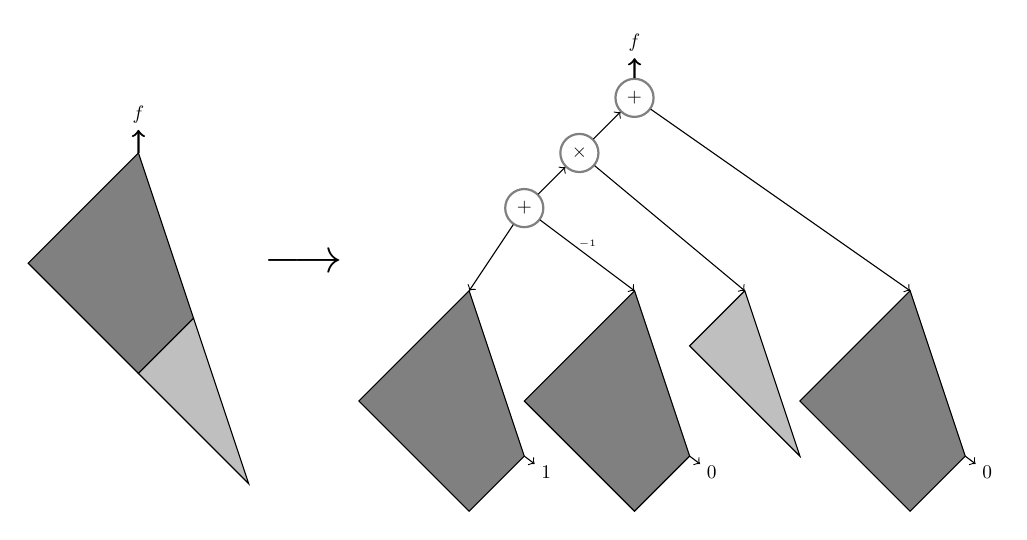
\begin{tikzpicture}[transform shape, scale=0.7]
  \draw[fill=gray] (-10,-2) -- ++(-2,-2) -- ++(2,-2) -- ++(1,1) -- cycle;
  \draw[fill=gray!50] (-9,-5) -- ++(1,-3) -- ++(-2,2) -- cycle;

    \node at (-10,-1.3) {$f$}
    edge[<-,thick] (-10,-2) ;

  
  \node at (-7,-4) {\Huge $\longrightarrow$};
  
  \node (ph) at (-1,0) {$f$};
  \node[gate] (root) at (-1,-1) {$+$}
  edge[thick,->] (ph)
  edge[->] (4,-4.5);
  \node[gate] (m1) at (-2,-2) {$\times$}
  edge[->] (root)
  edge[->] (1,-4.5);
  
  \draw[fill=gray] (4,-4.5) -- ++(-2,-2) -- ++(2,-2) -- ++(1,1) -- cycle;
  \node at  (5.4,-7.8) { $0$}
  edge[<-] (5,-7.5);
  
  \node[gate] (s1) at (-3,-3) {$+$}
  edge[->] (m1)
  edge[->] (-4,-4.5)
  edge[->] node[above] {\tiny $-1$} (-1,-4.5);
  
  \draw[fill=gray!50] (1,-4.5) -- ++(1,-3) -- ++(-2,2) -- cycle;
  
  
  \draw[fill=gray] (-4,-4.5) -- ++(-2,-2) -- ++(2,-2) -- ++(1,1) -- cycle;
  \node at  (-2.6,-7.8) { $1$}
  edge[<-] (-3,-7.5);
  
  \draw[fill=gray] (-1,-4.5) -- ++(-2,-2) -- ++(2,-2) -- ++(1,1) -- cycle;
  \node at  (0.4,-7.8) { $0$}
  edge[<-] (0,-7.5);
\end{tikzpicture}
\end{center}
\caption{Depth reduction for formulas}
\label{fig:formula-depth-red}
\end{figure}

\subsection{Depth reduction for arithmetic circuits}

The key point in the above depth reduction was that for any node $v$, the formulas $\Phi_v$ and $\hat{\Phi}_v(y)$ were disjoint. This however is not the case for general arithmetic circuits. Thus, it is not clear if we can find a node in the circuit such that the subcircuit under it has size between $s/3$ and $2s/3$. However, we do not really need to make the subcircuits have size drop by a constant factor, but any parameter dropping by a constant factor would be fine. One parameter that we could work with instead is the \emph{degree}. 


\subsubsection{Applying Brent's reduction with degree}

By Lemma~\ref{lem:homogenization}, we may assume that we have a homogeneous circuit $\Phi$ if size $s$ computing a homogeneous $n$-variate polynomial $f$ of degree $d$. Using a similar argument as in the proof of Lemma~\ref{lem:formula-depth-reduction}, we can find a node $v \in \Phi$ such that $\frac{d}{3} < \deg(v) \leq \frac{2d}{3}$. However, we cannot quite write $f$ as $A \cdot \Phi_v + B$ as we are now dealing with a circuit and there could be multiple paths from the root leading to $v$.

Consider the set of all nodes of such intermediate degree as $\mathcal{F}$:
\[
\mathcal{F} = \setdef{v\in \Phi}{\frac{d}{3} < \deg(v)\leq \frac{2d}{3}}
\]
Instead of expressing $f$ using a single $v\in \mathcal{F}$ as in Lemma~\ref{lem:formula-depth-reduction}, we shall express $f$ as a function of \emph{all} nodes in $\mathcal{F}$. 

\begin{claim}
If $\mathcal{F} = \inbrace{v_1,\dots, v_s}$, then $f$ may be written as
\begin{equation}\label{eqn:hyafil}
f \spaced{=} \sum_{i,j} A_{ij} \cdot \Phi_{v_i} \Phi_{v_j} \spaced{+} \sum_i B_i \cdot \Phi_{v_i}
\end{equation}
where $\deg(A_{ij}), \deg(B_i) \leq \frac{2d}{3}$ for all $i,j$. Moreover, each $A_{ij}$ and $B_i$'s may be computed by an arithmetic circuit of size at most $O(s)$. 
\end{claim}
\begin{proof}
From the circuit $\Phi$, construct the circuit $\Phi'$ that is obtained by removing the incoming edges of every $v_i \in \mathcal{F}$ thereby making these nodes as leaves as well. Then, $\Phi'$ computes a polynomial $f'(x_1,\dots x_n, v_1,\dots, v_s)$ satisfying 
\[
f \spaced{=} f'(x_1,\dots, x_n, \Phi_{v_1},\dots, \Phi_{v_s}).
\]
Because of the degree of each $v_i$, we easily obtain that the degree of $f'$ in the $v_i$ variables must be at most $2$, and each coefficient $A_{ij}$ or $B_i$ cannot have degree more than $2d/3$. Further, obtaining the $A_{ij}$'s and $B_i$'s from $\Phi'$ is a simple exercise. 
\end{proof}

Since every polynomial appearing in \eqref{eqn:hyafil} is computable by size at most $\poly(s)$ and has degree at most $2d/3$, we may apply induction as earlier. Thus,
\begin{eqnarray*}
\mathrm{Depth}(d) & = & \mathrm{Depth}(2d/3) \quad + 2\\
\implies \mathrm{Depth}(d) & = & O(\log d)
\end{eqnarray*}
Unfortunately, the size of the resulting circuit could be as large as $s^{O(\log d)}$.  This reduction is along the lines of Hyafil~\cite{Hyafil1978}. 

Notice that in this reduction, the final circuit we obtain is in fact an arithmetic formula of size $s^{O(\log d)}$ and depth $O(\log d)$ (assuming that addition gates can have unbounded fan-in; with bounded fan-in addition gates, the depth would be $O(\log d \cdot \log s)$). Valiant, Skyum Berkowitz and Rackoff \cite{vsbr83} showed that we can attain a similar depth reduction to $O(\log d)$ depth while keeping the size polynomial. 


\subsubsection{Depth reduction of \cite{vsbr83}}


This section shall be devoted to the proof of the remarkable theorem of Valiant, Skyum, Berkowitz and Rackoff.\footnote{The proof described here follows the structure of a subsequent result \cite{ajmv98}, and not the original proof, although both proofs are quite similar.}


\begin{theorem}[\cite{vsbr83,ajmv98}]\label{thm:vsbr}
  Let $f$ be an $n$-variate degree $d$ polynomial computed by an
  arithmetic circuit $\Phi$ of size $s$. Then there is an arithmetic
  circuit $\Phi'$ computing $f$ and has size $s' = \poly(s,n,d)$ and
  depth $O(\log d)$.
\end{theorem}

We may assume without loss of generality that $\Phi$ is a homogeneous circuit. We will also assume that all multiplication gates in $\Phi$ have fan-in at most $2$, and also that the degree of the right child of any multiplication gate is at least as large as the degree of the left child. Such circuits are also referred to as \emph{right heavy} circuits. We shall need the following definition of gate quotients.

\begin{definition}\label{defn:gate-quotient}
For any pair of gates $u,v$, the polynomial $[u:v]$ is defined as follows:
\begin{enumerate}
\item If $u$ and $v$ are the same nodes, then $[u:v] = 1$. 
\item If $u$ is a leaf, and $u\neq v$, then $[u:v] = 0$. 
\item If $u = u_1 + u_2$, then $[u:v] = [u_1:v] + [u_2:v]$.
\item If $u = u_1 \times u_2$, then $[u:v] = [u_1] \cdot [u_2 : v]$. 
\end{enumerate}
\end{definition}

It is easy to see that $[u:v]$ is a homogeneous polynomial of degree $\deg(u) - \deg(v)$. 
To understand this definition better, consider the case of a formula instead of a circuit. Then for any node $u$, and another node $v$ in the sub-formula rooted at $u$, the polynomial $[u]$ can depends on $[v]$ linearly as $[u] = A [v] + B$ for some $A,B$. In this setting, $[u:v] = A$. For circuits however, there could be multiple paths from $u$ leading to $v$. One possible alternate definition could have been to \emph{differentiate} $[u]$ by $[v]$ but this would require some additional care. The above definition makes sure we are exploring only one of the children of any multiplication gate, and yields a much simpler proof. 

\begin{definition}[Frontier]\label{defn:frontier}
For any parameter $a$, define the \emph{frontier at degree $a$} as
\[
\mathcal{F}_a \quad=\quad \setdef{v}{\deg(v) \geq a\;,\; \deg(v_L), \deg(v_R) < a}
\]
That is, $\mathcal{F}_a$ are the deepest nodes in the circuit that have degree at least $a$. 
\end{definition}

Note that from the above definition, all frontier nodes are multiplication gates (since we are working with a homogeneous circuit). Also, if $v_1,v_2$ are two distinct nodes in $\mathcal{F}_a$, then $v_1$ does not occur in the sub-circuit rooted at $v_2$ (and vice-versa). 

\begin{observation}\label{obs:vsbr-antichain}
If a node $v$ does not occur in the sub-formula rooted at $u$, then $[u:v] = 0$. In particular, if $u\neq v\in \mathcal{F}_a$ for some $a$, then $[u:v]=0$.
\end{observation}

The following is the key lemma for the depth reduction. 

\begin{lemma}
Suppose $\Phi$ is a homogeneous, right-heavy circuit. Let $a$ be a parameter such that $\deg(u) \geq a$. Then,
\begin{equation}\label{eqn:vsbr-for-u}
[u]\spaced{=} \sum_{w\in \mathcal{F}_a} [u:w] \cdot [w]
\end{equation}
Also, if $u,v$ are nodes such that $\deg(u) \geq a > \deg(v)$, then
\begin{equation}\label{eqn:vsbr-for-uv}
[u:v] \spaced{=} \sum_{w\in \mathcal{F}_a} [u:w] [w:v]
\end{equation}
\end{lemma}
\begin{proof}
The proof would be by induction on the depth of $u$. Note that if $u = u_1 + u_2$, then it follows immediately that 
\begin{eqnarray*}
  [u] &=& [u_1] + [u_2] \\
  &=& \sum_{w\in \mathcal{F}_a} \inparen{[u_1: w]\cdot [w]  + [u_2:w]\cdot [w]}\quad\text{(inductive hypothesis)}\\
  &=& \sum_{w\in \mathcal{F}_a} [u:w] \cdot [w] \quad\text{(Definition~\ref{defn:gate-quotient})}
\end{eqnarray*}
\begin{eqnarray*}
  [u:v] &=& [u_1:v] + [u_2:v] \\
  &=& \sum_{w\in \mathcal{F}_a} \inparen{[u_1: w]\cdot [w:v]  + [u_2:w]\cdot [w:v]}\quad\text{(inductive hypothesis)}\\
  &=& \sum_{w\in \mathcal{F}_a} [u:w] \cdot [w:v] \quad\text{(Definition~\ref{defn:gate-quotient})}
\end{eqnarray*}
Suppose $u = u_1 \times u_2$. If $\deg(u_2) \geq a$ as well, then by induction we have
\begin{eqnarray*}
[u] &=& [u_1] \cdot [u_2]\\
    &=& [u_1] \cdot \inparen{\sum_{w\in \mathcal{F}_a} [u_2:w]\cdot [w]} \quad\text{(inductive hypothesis)}\\
    &=& \sum_{w\in \mathcal{F}_a}([u_1]\cdot [u_2:w]) \cdot [w] = \sum_{w\in \mathcal{F}_a}[u:w] \cdot [w]\quad\text{(Definition~\ref{defn:gate-quotient})}
\end{eqnarray*}
\begin{eqnarray*}
[u:v] &=& [u_1] \cdot [u_2:v]\\
    &=& [u_1] \cdot \inparen{\sum_{w\in \mathcal{F}_a} [u_2:w]\cdot [w:v]} \quad\text{(inductive hypothesis)}\\
    &=& \sum_{w\in \mathcal{F}_a}([u_1]\cdot [u_2:w]) \cdot [w:v] = \sum_{w\in \mathcal{F}_a}[u:w] \cdot [w:v]\quad\text{(Definition~\ref{defn:gate-quotient})}
\end{eqnarray*}

If $\deg(u_2) < a$, then note that $u \in \mathcal{F}_a$. Hence,
\begin{eqnarray*}
\sum_{w\in \mathcal{F}_a} [u:w] \cdot [w] &=& [u:u] \cdot [u] \spaced{+}\sum_{\substack{w\in \mathcal{F}_a\\w\neq u}} [u:w] \cdot [w] \spaced{=} [u] \spaced{+} 0\\
\sum_{w\in \mathcal{F}_a} [u:w] \cdot [w:v] &=& [u:u] \cdot [u:v] \spaced{+}\sum_{\substack{w\in \mathcal{F}_a\\w\neq u}} [u:w] \cdot [w:v] \spaced{=} [u:v] \spaced{+} 0
\end{eqnarray*}
as $[u:w] = 0$ for all $u\neq w \in \mathcal{F}_a$ (Observation~\ref{obs:vsbr-antichain}).
\end{proof}

Now we are ready to write down the depth reduced circuit. The original proof of \cite{vsbr83} follows a bottom-up approach, but it would be more useful to us to take a top-down approach (as in \cite{ajmv98}) to obtain some additional structural properties that we would require. \\

\begin{theorem}
Let $\Phi$ be a homogeneous, left-heavy circuit of size $s$ computing an $n$-variate degree $d$ polynomial. Then, there is a circuit $\Phi'$ of size $\poly(s)$ with the following properties:
\begin{enumerate}
\item For every $u\in \Phi$, there is a node in $\Phi'$ that computes $[u]$.
\item For every $u,v\in \Phi$, there is a node in $\Phi'$ that computes $[u:v]$. 
\item All addition gates in $\Phi'$ have fan-in at most $s^2$. 
\item All multiplication gates in $\Phi'$ have fan-in at most $5$. 
\item For every multiplication gate in $\Phi'$, all its children have at most half its degree. 
\end{enumerate}
\end{theorem}
\begin{proof}
All nodes $[u]$ and $[u:v]$ of degree at most $1$ are linear polynomials, and hence can are written down explicitly in $\Phi'$. 

For any node $u\in \Phi$, let $\mathcal{F}(u) = \mathcal{F}_a$ for $a = \deg(u)/2$. Thus by \eqref{eqn:vsbr-for-u},
\begin{eqnarray*}
[u] & = & \sum_{w\in \mathcal{F}(u)} [u:w] \cdot [w]\\ 
    & = & \sum_{w\in \mathcal{F}(u)} [u:w] \cdot [w_L] \cdot [w_R]
\end{eqnarray*}
Note that by the choice of $a$, all the terms on the RHS have degree at most $\deg(u)/2$. 

For any pair of nodes $u,v\in \Phi$, let $\mathcal{F}(u,v) = \mathcal{F}_a$ for $a = (\deg(u) + \deg(v))/2$. By \eqref{eqn:vsbr-for-uv},
\begin{eqnarray*}
[u:v] & = & \sum_{w\in \mathcal{F}(u,v)} [u:w] \cdot [w:v]\\ 
    & = & \sum_{w\in \mathcal{F}(u,v)} [u:w] \cdot [w_L] \cdot [w_R:v]
\end{eqnarray*}
Again by the choice of $a$, the degree of $[u:w]$ and the degree of $[w_R:v]$ is at most $(\deg(u) - \deg(v))/2$. The degree of $[w_L]$ however could be as large as $\deg(u) - \deg(v)$. Nevertheless, we can use the above expansion once more to write it as
\begin{eqnarray*}
  [u:v] & = & \sum_{w\in \mathcal{F}(u,v)} [u:w] \cdot [w_L] \cdot [w_R:v]\\
        & = & \sum_{w\in \mathcal{F}(u,v)} [u:w] \inparen{\sum_{p \in \mathcal{F}(w_L)} [w_L:p] \cdot [p_L] \cdot [p_R]}\cdot [w_R:v]\\
        & = & \sum_{w\in \mathcal{F}(u,v)}\sum_{p\in \mathcal{F}(w_L)} [u_w] \cdot  [w_L:p] \cdot [p_L] \cdot [p_R]\cdot [w_R:v]
\end{eqnarray*}
Now all the terms on the RHS have degree at most $(\deg(u) - \deg(v))/2$ as required. 
\end{proof}

% \newpage



% \begin{theorem}[\cite{vsbr83}]\label{thm:vsbr}
% Let $f$ be an $n$-variate degree $d$ polynomial computed by an arithmetic circuit $\Phi$ of size $s$. Then, there is an arithmetic circuit $\Phi'$ computing $f$ and has size $s' = \poly(s,n,d)$ and depth $O(\log d)$. 
% \end{theorem}

% By Lemma~\ref{lem:homogenization}, we may assume without loss of generality that $\Phi$ is a homogeneous circuit. We will also assume that in $\Phi$, all multiplication gates have fan-in at most $2$ (this might increase the depth of $\Phi$ by a factor of $\log s$, but this would not hurt us). Now, we can find a similar ``$\inparen{\frac{1}{3},\frac{2}{3}}$ separator'' as in the proof of Lemma~\ref{lem:formula-depth-reduction}, but based on degree instead of size. 

% \begin{claim}
% Let $\Phi$ be a homogeneous arithmetic circuit computing a homogeneous degree $d$ polynomial, where each multiplication gate has fan-in at most $2$. Then, there exists a node $v$ that computes a polynomial of degree $d'$ satisfying $d/3 \leq d' \leq 2d/3$. 
% \end{claim}

% The proof is exactly the same, except now you take a path from root to leaf by always going through the child of larger degree. What can we say about replacing the entire sub-circuit at $v$ by a new variable $y$? This runs in to some immediate problems. What if there was a node $w$ in the subcircuit at $v$, which is maybe connected to other nodes in $\Phi$? Also, the polynomial $\hat{\Phi}_v(y)$ could continue to have degree as large as $d$. Thus it is not clear if this approach would help us make progress. 

% The cause of all these problems stems because the node $v$ could reached from the root through multiple paths, and hence needs to be treated with care. However, with a little more care, we can still mimic the earlier depth reduction for formulas. \\

% Let us go over every gate in $\Phi$, and reorder the children so that the children are sorted in decreasing order of degrees (with the left child being the one with largest degree). We shall call such circuits as \emph{left-heavy} circuits. Note that the proof of the claim above yields such a node $v$ on the left-most path of $\Phi$. 

% Since any polynomial is a sum of monomials, it would be useful to break the computation by an arbitrary circuits by a sum of smaller computations each corresponding to a monomial. The following definition does just that. 

% \begin{definition}[Proof trees]\label{defn:proof-tree}
% A \emph{proof tree} of an arithmetic circuit $C$ is a sub-graph $T$ obtained as follows:
% \begin{itemize}
% \item The root of $C$ is in $T$.
% \item For every addition gate $g\in T$, the subgraph $T$ also contains \emph{exactly one} of its children.
% \item For every multiplication gate $g\in T$, the subgraph $T$ also contains \emph{both} its children. 
% \end{itemize}
% \end{definition}

% A proof tree naturally computes a single monomial, and is a minimal witness that a certain monomial is computed in by the circuit. (It is however possible that the same monomial can be computed by multiple proof trees and there could be several cancellations.)

% A very natural question at this point is why is a \emph{proof tree} a tree! It isn't clear from the above definition but note that all proof trees of a homogeneous circuit $C$ (computing a degree $d$ polynomial) computes a monomial of degree $d$. Thus, the number of multiplication gates in any proof tree is at most $d$. Thus, we may unravel any proof tree $T$ to an actual tree $T$ while not increasing the size by much. Thus, without loss of generality, we may assume that all proof trees of $C$ are unravelled to indeed be trees. 

% We shall denote the set of all proof trees of a circuit $C$ by $\mathrm{ProofTrees}(C)$. Also, for any node $u\in C$, we shall use $\mathrm{ProofTree}(u)$ to refer to the set of all proof trees rooted at $u$. Further, for any proof tree $T$, we shall use $\mathrm{eval}(T)$ to denote  the  \emph{monomial computed by $T$}. Thus, if $f$ is the polynomial computed by a circuit $C$, then
% \[
% f\spaced{=} \sum_{T\in \mathrm{ProofTrees}(C)} \mathrm{eval}(T)
% \]

% With this definition, we can now apply a Brent-like argument on \emph{proof trees} rather than the actual circuit itself. Recall that in the proof of Lemma~\ref{lem:formula-depth-reduction}, we expressed $\Phi$ as a linear function of $A \Phi_v + B$. The following notation captures the quotient $A$, but now in the case of general circuits via the notation of proof trees. 

% \begin{definition}[Proof tree quotients]
% For any proof tree $T$, and a node $v$, define the operation $\mathrm{snip}_v(T)$ as
% \begin{itemize}
%   \item If $v$ does not appear in the left-most path of $T$, then $\mathrm{snip}_v(T) = 0$
%   \item If $v$ does appear in the left-most path of $T$, then $\mathrm{snip}_v(T)$ refers to the tree obtained by replacing the node $v$ on the left-most path by a leaf labelled $1$. 
% \end{itemize}
% For any two nodes $u$ and $v$ in the circuit $C$, the polynomial $[u:v]$ is defined as
% \[
% [u:v] \spaced{=} \sum_{T \in \mathrm{ProofTrees}(u)} \mathrm{eval}(\mathrm{snip}_v(T))
% \]
% \end{definition}

% Intuitively, $[u:v]$ refers to the \emph{suffix} of $v$ in the computation at $u$. By only snipping off $v$ from the left-most path, this allows us to get a better control with the issue of $v$ occurring multiple times in the proof tree. For a formula $\Phi$, the polynomial $[\Phi:v]$ would refer to $\hat{\Phi}_v(1)$. Note that $[u:v]$ is a polynomial of degree $\deg(u) - \deg(v)$. \\

% The next thing we would like to do using the above notation is to rewrite the polynomial computed at $u$ by a sum involving several $[u:v_i]$s for suitable choice of $v_i$. To do this, we need to identify a set of nodes $\inbrace{v_i}$ such that the left-most path of every proof tree $T$ passes through exactly one $v_i$ from this set. One example of such a set is just the set of leaves. Thus, we can express the polynomial computed at any node $u$ as
% \[
% [u] \spaced{=} \sum_{i} [u:x_i] \cdot x_i
% \]
% In fact, a more general construction could be defined for any parameter $t$ as
% \[
% \mathcal{F}_t  \spaced{=} \setdef{w\in C}{\deg(w) \geq t \spaced{\&} \deg(w_L) < t}
% \]
% where $w_L$ refers to the left child of $w$. 

% \begin{observation}\label{obs:vsbr-split-threshold}
% For any node $u$, and a parameter $t$ such that $t \leq \deg(u)$, the left-most path of any proof tree $T$ of $u$ passes through exactly one node in $\mathcal{F}_t$. 
% \end{observation}

% Hence, $[u]$ can be expressed as follows:
% \begin{equation}\label{eqn:vsbr-split-threshold}
% [u] \spaced{=} \sum_{v\in \mathcal{F}_t} [u:v] \cdot [v]
% \end{equation}
% as long as $t \leq \deg(u)$. When we have nodes $u,v \in C$, we shall use $\mathrm{Frontier}(u)$ to refer to $\mathcal{F}_t$ where $t = \deg(u)/2$ and $\mathrm{Frontier}(u:v)$ to refer to $\mathcal{F}_t$ for $t = \deg(u:v)/2$. These are the frontiers that cut the appropriate tree into `half'. It is worth noting that all nodes in $\mathcal{F}_t$ must be multiplication gates (since the children have strictly smaller degree). 


% \begin{observation}
% The left-most path of any proof tree $T$ of $u$ passes through exactly one node in $\mathrm{Frontier}(u)$. The same applies to $\mathrm{Frontier}(u:v)$ as well. 
% \end{observation}

% With this observation, we have the sums we were looking for. 

% \begin{eqnarray}\label{eqn:VSBR-split-frontier}
% \text{For any $u\in C$,}\quad\quad [u] &=& \sum_{v\in \mathrm{Frontier}(u)} [u:v]\cdot [v] \label{eqn:VSBR-split-frontier-u}\\
% \text{For any $u,v\in C$,}\quad\quad [u:v] &=& \sum_{w\in \mathrm{Frontier}(u:v)} [u:w]\cdot [w:v] \label{eqn:VSBR-split-frontier-u:v}
% \end{eqnarray}

% With these in hand, we can now describe the depth-reduced circuit of \cite{vsbr83}. \\

% For each $u \in C$, the circuit $C'$ has a node computing $[u]$, and for every pair of nodes $u,v\in C$, there is a node in $C'$ computing $[u:v]$. To describe how $[u]$ is computed in $C'$, start with equation \eqref{eqn:VSBR-split-frontier-u}
% \begin{eqnarray*}
% [u] &=& \sum_{v\in \mathrm{Frontier}(u)} [u:v]\cdot [v]\\
%  & = & \sum_{v\in \mathrm{Frontier}(u)} [u:v] \cdot [v_L] \cdot [v_R]
% \end{eqnarray*}
% Note that since $v\in \mathrm{Frontier}(u)$, we have that $\deg(v) \geq \deg(u)/2$ and $\deg(v_R),\deg(v_L) < \deg(u)/2$. Thus each of the three terms in every summand of the above equation has degree at most half the degree $u$. The computation of $[u:v]$'s are a little more involved. By equation \eqref{eqn:VSBR-split-frontier-u:v}, we have
% \begin{eqnarray*}
% [u:v] &=& \sum_{w\in \mathrm{Frontier}(u:v)} [u:w]\cdot [w:v]\\
%       &=& \sum_{w\in \mathrm{Frontier}(u:v)} [u:w]\cdot [w_R]\cdot  [w_L:v]
% \end{eqnarray*}
% Since every $w \in \mathrm{Frontier}(u:v)$, we have that $\deg(u:w),\deg(w_L:v) \leq \deg(u:v)/2$. The issue is that $[w_R]$ could have pretty large degree. To see this, note that $w$ is a node of degree between $\deg(u)$ and $\deg(v)$. Thus, it is possible that $(u:w)$ and $(w_L:v)$ have very small degree and $\deg(w_R)$ could be as large as $\deg(u:v)$. However, we can expand $[w_R]$ using \eqref{eqn:VSBR-split-frontier-u} and we would then have what we want. 
% \begin{eqnarray*}
% [u:v] &=& \sum_{w\in \mathrm{Frontier}(u:v)} [u:w]\cdot [w_R]\cdot  [w_L:v]\\
%       &=& \sum_{w\in \mathrm{Frontier}(u:v)} [u:w]\cdot \inparen{\sum_{p \in \mathrm{Frontier}(w_L)} [w_R:p] \cdot [p_L] \cdot [p_R]} \cdot  [w_L:v]
% \end{eqnarray*}
% Observe that we have $\deg (u:w), \deg(w_L:v) \leq \deg(u:v)/2$ from earlier, and we also have
% \begin{eqnarray*}
% \deg(u:w),\deg(w_L:v) & \leq &\frac{\deg(u:v)}{2}\\
% \deg(w_R:p),\deg(p_L),\deg(p_R) & \leq & \frac{\deg(w_R)}{2}\\
%  & \leq & \frac{\deg(u:v)}{2}
% \end{eqnarray*}
% Thus, once again, we are in the situation where all the factors in the RHS have at most half the degree of the RHS. Thus, this shows that every $(u:v)$ can be computed by an arithmetic circuit $C'$ of size $\poly(s)$ and depth $O(\log d)$. In particular, $f = [\mathrm{root}]$ can be computed be computed by $C'$, as claimed. \qed {(\footnotesize Theorem~\ref{thm:vsbr})}\\

\begin{remark}\label{remark:vsbr}
From the proof above, we can see that the resulting circuit $\Phi'$ has useful structural properties. 
\begin{itemize}
  \item The circuit is homogeneous. 
  \item Addition gates have fan-in bounded by $\poly(s)$. 
  \item Multiplication gates have fan-in bounded by $5$. 
  \item If $u$ is any multiplication gate, then all its children $v$ satisfy $\deg(v)\leq \deg(u)/2$. 
\end{itemize}
\end{remark}

These additional properties would be useful in the next section, where we shall squash $\Phi'$ down to a depth four circuit!

\subsection{Reduction to depth four circuits}

One of the consequence of a depth reduction such as Theorem~\ref{thm:vsbr} is that proving lower bounds for general circuits is reduced to the task of proving lower bounds for $O(\log d)$ depth circuits. 

\begin{corollary}\label{cor:vsbr-contra}
If $f$ is an $n$-variate degree $d$ polynomial that requires super-polynomial (in $n$ and $d$) size circuits of $O(\log d)$ depth to compute it, then any general arithmetic circuit computing $f$ must also be of super-polynomial size. 
\end{corollary}

But, optimistically, we would expect that the \emph{right} lower bound must be truly exponential, and not merely super-polynomial. Keeping that in mind, a depth reduction even with a slightly super-polynomial blow-up might be useful in this regard. This line was first pursued by Agrawal and Vinay \cite{av08}, and the result was subsequently strengthened by Koiran \cite{koiran} and Tavenas~\cite{Tav13}. 

\begin{theorem}[\cite{av08,koiran,Tav13}] \label{thm:av}
Let $f$ be an $n$-variate degree $d$ polynomial computed by a size $s$ arithmetic circuit. Then for any $0< t \leq d$, $f$ can be equivalently computed by a homogeneous $\SPSP^{[t]}$ circuit of top fan-in $s^{O(d/t)}$ and size $s^{O(t + d/t)}$. 
\end{theorem}

If we were to optimize the size of the final depth four circuit, then we should choose $t = \sqrt{d}$ to get a $\SPSP^{[t]}$ circuit of size $s^{O(\sqrt{d})}$. Note that this implies that if we could prove a lower bound of $n^{\omega(\sqrt{d})}$ for such $\SPSP^{[\sqrt{d}]}$ circuits, then we would have proved a lower bound for general circuits! In fact, in the recent past, we have come pretty close to the required threshold and we shall see them in the later chapters. \\

In this section, we shall see a proof of Theorem~\ref{thm:av} but this is not the original proof of Tavenas~\cite{Tav13}. We shall see an alternate proof by \cite{saptharishivinay14}, which I find more insightful. 

\begin{proofof}{Theorem~\ref{thm:av}}
Let $C$ be the $O(\log d)$ depth  circuit computing $f$ obtained from Theorem~\ref{thm:vsbr} applied on the size $s$ circuit computing $f$. Let $s'$ be the size of $C$. If $g$ is a polynomial computed at any intermediate node of $C$, then from the structure of $C$ (Remark~\ref{remark:vsbr}) we have a homogeneous expression
\begin{equation}\label{eqn:vsbr-expansion}
g \spaced{=} \sum_{i=1}^{s'} g_{i1} \cdot g_{i2} \cdot g_{i3} \cdot g_{i4} \cdot g_{i5} 
\end{equation}
where each $g_{ij}$ is computed by a node in $C$ as well, and $\deg(g_{ij}) \leq \deg(g)/2$. If we look at \eqref{eqn:vsbr-expansion} for $f$, then the RHS is a $\SPSP^{[d/2]}$ circuit of top fan-in $s'$ computing $f$. To obtain a $\SPSP^{[t]}$ circuit eventually, we shall do the following natural process. 
\begin{quote}
  For each summand $g_{i1}\dots g_{ir}$ in the RHS, if the largest degree $g_{ij}$ has degree more than $t$, expand that $g_{ij}$ in-place using \eqref{eqn:vsbr-expansion}. 
  
  Repeat this process until all $g_{ij}$'s on the RHS have degree at most $t$. 
\end{quote}

Note that in each iteration of the above procedure, we increase the top fan-in by a multiplicative factor of $s'$, and what we gain is that some the terms in the RHS would now have smaller degrees. If we could show that the in $O(d/t)$  iterations  all terms on the RHS have degree at most $t$, then we would have obtained an $\SPSP^{[t]}$ circuit of top fanin $s'^{O(d/t)}$ computing $f$. \\

To bound the number of iterations, let us count the number of terms of degree more than $t/8$ in each term. Note that since we would always maintain homogeneity, the number of terms of degree  $t/8$ or more in any summand  is at most $8d/t$. Thus, it suffices to show that each iteration increases the number of terms of degree $t/8$ by at least one. 

Note that in \eqref{eqn:vsbr-expansion}, if $\deg(g) = d'$ then the largest degree term of any summand on the RHS is at least $d'/5$ (since the sum of the degrees of the five terms must add up to $d'$). Also, the largest degree term can have degree at most $d'/2$. Hence there must be at least $d'/2$ degree contributed by the other four factors in each term. This implies that the second largest factor in each summand has degree at least $d'/8$. Therefore, as long as we are expanding factors using \eqref{eqn:vsbr-expansion} of degree more than $t/8$, we are guaranteed that each new term has at least one more factor of degree more than $t/8$. As argued earlier, we can never have more than $8d/t$ such terms in any summand and this bounds the number of iterations by $8d/t$. 

Thus, when the above procedure stops, we have an $\SPSP^{[t]}$ circuit of top fan-in $s'^{O(8d/t)} = s^{O(d/t)}$. Observing that any polynomial of degree $t$ can have at most $n^t$ monomials, we get that the size of the circuit overall is at most $s^{O(t + d/t)}$. 
\end{proofof}

Thus, proving a ``good enough'' top fanin (or size) lower bound for the class of $\SPSP^{[t]}$ circuit would suffice for proving lower bounds for general circuits. We would be using this fact quite a lot so we state this explicitly as a corollary. 

\begin{corollary}\label{cor:av}
If $f$ is an $n$-variate degree $d$ polynomial that requires homogeneous $\SPSP^{[t]}$ circuits of top fan-in $n^{\omega(d/t)}$ to compute it, then $f$ requires general arithmetic circuits of size $n^{\omega(1)}$ to compute it. 
\end{corollary}

\begin{exercise}
Define the product-depth of any circuit to be the maximum number of multiplication gates encountered on any root-to-leaf path. 

Show that for any polynomial $n$-variate degree $d$ polynomial $f$ that can be computed by a size $s$ arithmetic circuit, there is a circuit $\Phi'$ of size $s^{O(d^{1/\Delta})}$ and product depth $\Delta$ computing $f$. 
\end{exercise}

\subsection*{Further depth reductions}

There have been some further depth reductions results, but we shall defer that to later in the interest of presenting more insight and intuition. They would be better placed after we have seen a few of the recent lower bounds for restricted depth four circuits. We now proceed to see some lower bounds. 




%%% Local Variables: 
%%% mode: latex
%%% TeX-master: "main"
%%% End: 

\part{Classical lower bounds}

\chapter{Lower bounds for general circuits and formulas}\label{chap:gen-ckt-formulas}

Despite several attempts by various researchers to prove lower bounds for arithmetic circuits or formulas, we only have very mild lower bounds for general circuits or formulas thus far. In this chapter, we shall look at the two  modest lower bounds for general circuits and formulas. 

\section{Lower bounds for general circuits}\label{sec:baur-strassen}

The only super-linear lower bound we currently know for general arithmetic circuits is the following  result of Baur and Strassen \cite{BS83}.

\begin{theorem}[\cite{BS83}]\label{thm:baur-strassen}
  Any fan-in $2$ circuit that computes the polynomial $f = x_1^{d+1} + \dots + x_n^{d+1}$ has $\Omega(n\log d)$ edges. 
\end{theorem}


\subsection{An exploitable weakness}

Without loss of generality, let us assume that the circuit is a fan-in $2$ circuit. This would allow us to talk in terms of the number of nodes instead of edges. 

Each gate of the circuit $\Phi$ computes a local operation on the two children. To formalize this, define a new variable $y_g$ for every gate $g \in \Phi$. Further, for every gate $g$ define a quadratic equation $Q_g$ as
$$
Q_g = \begin{cases} y_g - (y_{g_1} + y_{g_2}) & \text{if $g = g_1 + g_2$}\\
  y_g - (y_{g_1}\cdot y_{g_2}) & \text{if $g = g_1 \cdot g_2$}.
\end{cases}
$$
Further if $y_o$  corresponds to the output gate, then the system of equations
$$\setdef{Q_g = 0}{g\in \Phi} \spaced{\union} \inbrace{y_{o} = 1}$$
completely characterize the computations of $\Phi$ that results in an output of $1$. 

The same can also be extended for \emph{multi-output} circuits that compute several polynomials simultaneously. In such cases, the set of equations
$$\setdef{Q_g = 0}{g\in \Phi} \spaced{\union} \setdef{y_{o_i} = 1}{i=1, \ldots, n}$$
completely characterize computations that result in an output of all ones. The following classical theorem allows us to bound the number of  common roots to a system of polynomial equations. 

\begin{theorem}[\Bezout's theorem]
  Let $g_1,\dots, g_r \in \F[X]$ such that $\deg(g_i) = d_i$ such that the number of common roots of $g_1=\dots=g_r = 0$ is finite. Then, the number of common roots (counted with multiplicities) is bounded by $\prod d_i$.
\end{theorem}

Thus in particular, if we have a circuit $\Phi$ of size $s$ that \emph{simultaneously} computes $\inbrace{x_1^d, \dots,x_n^d}$, then we have $d^n$ inputs that evaluate to all ones (where each $x_i$ must be  a $d$-th root of unity). Hence, \Bezout's theorem implies that
$$
2^s\spaced{\geq} d^n \spaced{\quad\implies\quad} s \spaced{=} \Omega(d\log n).
$$

Observe that $\inbrace{x_1^d,\dots, x_n^d}$ are all first-order derivatives of $f = x_1^{d+1}+\dots+x_n^{d+1}$ (with suitable scaling). A natural question here is the following --- if $f$ can be computed an arithmetic circuit of size $s$, what is the size required to compute all first-order partial derivatives of $f$ simultaneously? The \naive approach of computing each derivative separately results in a circuit of size $O(s\cdot n)$. Baur and Strassen \cite{BS83} show that we can save a factor of $n$.

\begin{lemma}[\cite{BS83}]\label{lem:baur-strassen}
  Let $\Phi$ be an arithmetic circuit of size $s$ and fan-in $2$ that computes a polynomial $f\in \F[X]$. Then, there is a multi-output circuit  of size $O(s)$ computing all first order derivatives of $f$.
\end{lemma}

Note that this immediately implies that any circuit computing $f = x_1^{d+1} + \dots + x_n^{d+1}$ requires size $\Omega(d\log n)$ as claimed by Theorem~\ref{thm:baur-strassen}. 


\subsection{Computing all first order derivatives simultaneously}

Since we are working with fan-in $2$ circuits, the number of edges is at most twice the size. Hence let $s$ denote the number of edges in the circuit $\Phi$, and we shall prove by induction that all first order derivatives of $\Phi$ can be computed by a circuit of size at most $5s$. Pick a non-leaf node $v$ in the circuit $\Phi$ closest to the leaves with both its children being variables, and say $x_1$ and $x_2$ are the variables feeding into $v$. In other words, $v = x_1 \odot x_2$ where $\odot$ is either $+$ or $\times$.

Let $\Phi'$ be the circuit obtained by deleting the two edges feeding into $v$, and replacing $v$ by a new variable. Hence, $\Phi'$ computes a polynomial $f' \in \F[X\union \inbrace{v}]$ and has at most $(s-1)$ edges. By induction on the size, we can assume that there is a circuit $\mathbb{D}(\Phi')$ consisting of at most $5(s-1)$ edges that computes all the first order derivatives of $f'$.

Observe that since $f'\mid_{(v = x_1 \odot x_2)} = f(\vecx)$,  we have that 
$$
\parderiv{f}{x_i} \spaced{=}\inparen{\parderiv{f'}{x_i}}_{v = x_1 \odot x_2} \quad+\quad  \inparen{\parderiv{f'}{v}}_{v = x_1 \odot x_2}\inparen{\parderiv{(x_1 \odot x_2)}{x_i}}.
$$

Hence, if $v = x_1 + x_2$ then
\begin{eqnarray*}
  \parderiv{f}{x_1} & = & \inparen{\parderiv{f'}{x_1}}_{v=x_1 + x_2} +\quad \inparen{\parderiv{f'}{v}}_{v = x_1 + x_2}\\
  \parderiv{f}{x_2} & = & \inparen{\parderiv{f'}{x_2}}_{v=x_1 + x_2} +\quad \inparen{\parderiv{f'}{v}}_{v = x_1 + x_2}\\
  \parderiv{f}{x_i} & = & \inparen{\parderiv{f'}{x_i}}_{v=x_1 + x_2} \qquad\text{for $i>2$}.
\end{eqnarray*}
If $v = x_1 \cdot x_2$, then
\begin{eqnarray*}
  \parderiv{f}{x_1} & = & \inparen{\parderiv{f'}{x_1}}_{v=x_1 \cdot x_2} + \inparen{\parderiv{f'}{v}}_{v = x_1 \cdot x_2} \cdot x_2\\
  \parderiv{f}{x_2} & = & \inparen{\parderiv{f'}{x_2}}_{v=x_1 \cdot x_2} + \inparen{\parderiv{f'}{v}}_{v = x_1\cdot x_2}\cdot x_1\\
  \parderiv{f}{x_i} & = & \inparen{\parderiv{f'}{x_i}}_{v=x_1 \cdot x_2} \qquad\text{for $i>2$}.
\end{eqnarray*}

Hence, by adding at most $5$ additional edges to $\mathbb{D}(\Phi')$, we can construct $\mathbb{D}(\Phi)$ and hence size of $\mathbb{D}(\Phi)$ is at most $5s$. \qed (Lemma~\ref{lem:baur-strassen})

\section{Lower bounds for formulas}\label{sec:Kalorkoti}

This section would be devoted to the proof of Kalorkoti's lower bound
\cite{k85} for formulas computing $\Det_n$, $\Perm_n$.

\begin{theorem}[\cite{k85}]\label{thm:kalorkoti}
  Any arithmetic formula computing $\Perm_n$ (or $\Det_n$) requires
  $\Omega(n^3)$ size.
\end{theorem}

The exploitable weakness in this setting is again to use the fact that the polynomials computed at intermediate gates share many polynomial dependencies. 

\begin{definition}[Algebraic independence]
  A set of polynomials $\inbrace{f_1,\dots, f_m}$ is said to be
  \emph{algebraically independent} if there is no non-trivial polynomial 
  $H(z_1,\dots, z_m)$ such that $H(f_1,\dots, f_m)=0$. 

  The size of the largest algebraically independent subset of
  $\vecf=\inbrace{f_1,\dots, f_m}$ is called the \emph{transcendence
    degree} (denoted by $\mathrm{trdeg}(f)$).
\end{definition}

The proof of Kalorkoti's theorem proceeds by defining a \emph{complexity measure} using the above notion of algebraic independence. \\


{\bf The Measure:} 
For any subset of variables $Y\subseteq X$, we can write a polynomial
$f \in \F[X]$ of the form $f = \sum_{i=1}^s f_i \cdot m_i$ where $m_i$'s are
distinct monomials in the variables in $Y$, and $f_i \in
F[X \setminus Y]$. We shall denote by $\mathrm{td}_Y(f)$ the transcendence degree of $\inbrace{f_1,\dots, f_s}$


Fix a partition of variables $X = X_1 \sqcup \dots
\sqcup X_r$. For any polynomial $f\in \F[X]$, define the map $\CM{Kal}:\F[X]\rightarrow \Z_{\geq 0}$  as
$$
\CM{Kal}(f) \quad=\quad \sum_{i=1}^r \mathrm{td}_{X_i}(f).
$$

The lower bound proceeds in two natural steps:
\begin{enumerate}
\item Show that $\CM{Kal}(f)$ is \emph{small} whenever $f$ is computable by a \emph{small} formula. 
\item Show that $\CM{Kal}(\Det_n)$ is \emph{large}. 
\end{enumerate}

\subsection{Upper bounding $\CM{Kal}$ for a formula}

\begin{lemma}\label{lem:kal-upperbound}
  Let $f$ be computed by a fan-in two formula $\Phi$ of size $s$. Then
  for any partition of variables $X = X_1\sqcup \dots \sqcup X_r$, we
  have $\CM{Kal}(f) = O(s)$.
\end{lemma}
\begin{proof}
  For any node $v\in \Phi$, let $\textsc{Leaf}(v)$ denote the leaves
  of the subtree rooted at $v$ and let $\textsc{Leaf}_{X_i}(v)$ denote
  the leaves of the subtree rooted at $v$ that are in the part
  $X_i$. Since the underlying graph of $\Phi$ is a tree, it follows
  that the size of $\Phi$ is bounded by a twice the number of
  leaves. For each part $X_i$, we shall show that
  $\mathrm{td}_{X_i}(f) = O(\abs{\textsc{Leaf}_{X_i}(\Phi)})$, which
  would prove the required bound. \\

  Fix an arbitrary part $Y = X_i$. Define the following three 
  sets of nodes
  \begin{eqnarray*}
    V_0 & = & \setdef{v\in \Phi}{\abs{\textsc{Leaf}_{Y}(v)} = 0 \quad\text{and}\quad \abs{\textsc{Leaf}_{Y}(\textsc{Parent}(v))} \geq 2}\\
    V_1 & = & \setdef{v\in \Phi}{\abs{\textsc{Leaf}_{Y}(v)} = 1 \quad\text{and}\quad \abs{\textsc{Leaf}_{Y}(\textsc{Parent}(v))} \geq 2}\\
    V_2 & = & \setdef{v\in \Phi}{\abs{\textsc{Leaf}_{Y}(v)} \geq 2}.
  \end{eqnarray*}

  Each node $v\in V_0$ computes a polynomial in $f_v \in
  \F[X\setminus Y]$, and we shall replace the subtree at $v$ by a node
  computing the polynomial $f_v$. Similarly, any node $v\in V_1$
  computes a polynomial of the form $f^{(0)}_v + f^{(1)}_v y_v$ for some $y_v\in Y$
  and $f^{(0)}_v, f^{(1)}_v \in \F[X\setminus Y]$. We shall again replace the
  subtree rooted at $v$ by a node computing $f^{(0)}_v + f^{(1)}_v y_v$. 

  Hence, the formula $\Phi$ now reduces to a smaller formula $\Phi_Y$ with
  leaves  being the nodes in $V_0$ and $V_1$ (and nodes in $V_2$ are
  unaffected). We would like to show that the size of the reduced
  formula, which is at most twice the number of its leaves, is
  $O(\abs{\textsc{Leaf}_Y(\Phi)})$.

  \begin{observation}\label{obs:v1-bound}$\abs{V_1} \leq \abs{\textsc{Leaf}_Y(\Phi)}$.    
  \end{observation}
  \begin{myproof}{Obs}
    Each node in $V_1$ has a distinct leaf labelled with a variable in
    $Y$. Hence, $\abs{V_1}$ is bounded by the number of leaves
    labelled with a variable in $Y$.
  \end{myproof}
  
  This shows that the $V_1$ leaves are not too many. Unfortunately, we
  cannot immediately bound the number of $V_0$ leaves, since we could
  have a long chain of $V_2$ nodes each with one sibling being a $V_0$
  leaf. The following observation would show how we can eliminate such
  long chains.

  \begin{observation}\label{obs:same-leaf-collapse}
    Let $u$ be an arbitrary node, and $v$ be another node in the
    subtree rooted at $u$ with $\textsc{Leaf}_Y(u) =
    \textsc{Leaf}_Y(v)$. Then the polynomial $g_u$ computed at $u$ and
    the polynomial $g_v$ computed at $v$ are related as $g_u = f_1 g_v
    + f_2$ for some $f_1,f_2 \in \F[X\setminus Y]$.
  \end{observation}
  \begin{myproof}{Obs}
    If $\textsc{Leaf}_Y(u) =\textsc{Leaf}_Y(v)$, then every node on
    the path from $u$ to $v$ must have a $V_0$ leaf as the other child. The
    observation follows as all these nodes are $+$ or $\times$ gates.
  \end{myproof}

  Using the above observation, we shall remove the need for $V_0$
  nodes completely by augmenting each node $u$ (computing a polynomial
  $g_u$) in $\Phi_Y$ with polynomials $f_u^{(0)}, f_u^{(1)} \in \F[X\setminus Y]$
  to enable them to compute $f_u^{(1)}g_u + f_u^{(0)}$. Let this augmented formula be called $\hat{\Phi}_Y$. Using
  Observation~\ref{obs:same-leaf-collapse}, we can now contract any
  two nodes $u$ and $v$ with $\textsc{Leaf}_Y(u) =
  \textsc{Leaf}_Y(v)$, and eliminate all $V_0$ nodes
  completely. Since all $V_2$ nodes are internal nodes, the only leaves of the augmented formula $\hat{\Phi}_Y$ are in $V_1$. Hence, the size of the augmented formula $\hat{\Phi}_Y$ is  bounded by $2\abs{V_1}$, which is bounded by
  $2\abs{\textsc{Leaf}_Y(\Phi)}$ by Observation~\ref{obs:v1-bound}.\\

  Suppose $\Phi$ computes a polynomial $f$, which can be written as  $f
  = \sum_{i=1}^t f_i\cdot m_i$ with $f_i \in \F[X\setminus Y]$ and $m_i$'s being
  distinct monomials in $Y$. Since $\hat{\Phi}_Y$ also computes $f$, each $f_i$ is a polynomial
  combination of the polynomials $S_Y = \setdef{f_{u}^{(0)},
    f_{u}^{(1)}}{u\in \hat{\Phi}_Y}$. Since $\hat{\Phi}_Y$ consists of at
  most $2\abs{\textsc{Leaf}_Y(\Phi)}$ augmented nodes, we have that
  $\mathrm{td}_Y(f) \leq |S_Y| \leq 4\abs{\textsc{Leaf}_Y(\Phi)}$. Therefore, 
  $$
  \mathrm{td}_Y(f) \quad=\quad \mathrm{trdeg}\setdef{f_i}{i\in [t]} \quad\leq\quad 4\abs{\textsc{Leaf}_Y(\Phi)}
  $$
  Hence, 
  $$\CM{Kal}(\Phi) = \sum_{i=1}^r \mathrm{td}_{X_i}(f_i) \leq 4\inparen{\sum_{i=1}^r \abs{\textsc{Leaf}_{X_i}}} = O(s).
  $$
\end{proof}

\subsection{Lower bounding $\CM{Kal}(\Det_n)$}


\begin{lemma}\label{lem:kal-lowerbound}
  Let $X = X_1 \sqcup \dots \sqcup X_n$ be the partition as defined by
  $X_t = \setdef{x_{ij}}{i-j\equiv t\bmod{n}}$. Then,
  $\CM{Kal}(\Det_n) = \Omega(n^3)$.
\end{lemma}
\begin{proof}
  By symmetry, it is easy to see that $\text{td}_{X_i}(\Det_n)$ is
  the same for all $i$. Hence, it suffices to show that
  $\text{td}_{Y}(\Det_n) = \Omega(n^2)$ for $Y = X_n = \inbrace{x_{11},\dots, x_{nn}}$. 

  To see this, observe that the determinant consists of the monomials
  $\inparen{\frac{x_{11}\dots x_{nn}}{x_{ii}x_{jj}}}\cdot
  x_{ij}x_{ji}$ for every $i\neq j$. Hence, $\text{td}_{Y}(\Det_n)
  \geq \mathrm{trdeg}\setdef{x_{ij}x_{ji}}{i\neq j} =
  \Omega(n^2)$. Therefore, $\CM{Kal}(\Det_n) =
  \Omega(n^3)$.
\end{proof}

The proof of Theorem~\ref{thm:kalorkoti} follows from
Lemma~\ref{lem:kal-upperbound} and Lemma~\ref{lem:kal-lowerbound}.



%%% Local Variables: 
%%% mode: latex
%%% TeX-master: "main"
%%% End: 


\chapter{Some simple lower bounds}\label{chap:simpleLBs}


\section{``Natural'' proof strategies}\label{sec:roadmap}

The lower bounds presented in Section~\ref{chap:gen-ckt-formulas} proceeded by first identifying a \emph{weakness} of the model, and exploiting it in an explicit manner. More concretely, Section~\ref{sec:Kalorkoti} presents a promising strategy that could be adopted to prove lower bounds for various models of arithmetic circuits. The crux of the lower bound was the construction of a good map $\Gamma$ that assigned a number to every polynomial. The map $\CM{Kal}$ was useful to show a lower bound in the sense that any $f$ computable by a \emph{small} formula had \emph{small} $\CM{Kal}(f)$. In fact, all subsequent lower bounds in arithmetic circuit complexity have more or less followed a similar template of a ``natural proof''. More concretely, all the subsequent lower bounds we shall see would essentially follow the outlined plan.  

\begin{quote}
{\bf Step 1 (normal forms)} For every circuit in the circuit class $\mathcal{C}$ of interest, express the polynomial computed as a \emph{small sum of simple building blocks}. 
\end{quote}

For example, every $\Sigma\Pi\Sigma$ circuit is a \emph{small} sum of \emph{products of linear polynomials} which are the building blocks here. In this case, the circuit model naturally admits such a representation but we shall see other examples with very different representations as sum of building blocks. 

\begin{quote}
{\bf Step 2 (complexity measure)} Construct a map $\Gamma: \F[x_1,\dots, x_n] \rightarrow \Z_{\geq 0}$ that is \emph{sub-additive} i.e. $\Gamma(f_1 + f_2)\leq \Gamma(f_1) + \Gamma(f_2)$.
\end{quote}

In most cases, $\Gamma(f)$ is the rank of a large matrix whose entries are linear functions in the coefficients of $f$. In such cases, we immediately get that $\Gamma$ is sub-additive. 

The strength of the choice of $\Gamma$ is determined by the next step. 

\begin{quote}
{\bf Step 3 (potential usefulness)} Show that if $B$ is a \emph{simple building block}, then $\Gamma(B)$ is \emph{small}.
Further, check if $\Gamma(f)$ for a \emph{random polynomial} $f$ is large (potentially). 
\end{quote}

This would suggest that if any $f$ with large $\Gamma(f)$ is to be written as a sum of $B_1 + \dots + B_s$, then sub-additivity and the fact that $\Gamma(B_i)$ is small for each $i$ and $\Gamma(f)$ is large immediately imply that $s$ must be large. This implies that the complexity measure $\Gamma$ does indeed have a potential to prove a lower bound for the class. The next step is just to replace the \emph{random polynomial} by an explicit polynomial. 

\begin{quote}
{\bf Step 4 (explicit lower bound)} Find an explicit polynomial $f$ for which $\Gamma(f)$ is large. 
\end{quote} 



These are usually the steps taken in almost all the known arithmetic circuit lower bound proofs. The main ingenuity lies in constructing a useful complexity measure, which is really to design $\Gamma$ so that it is small on the \emph{building blocks}. \\

Of course, there could potentially be lower bound proofs that do not follow the road-map outlined. For instance, it could be possible that $\Gamma$ is not small for a random polynomial, but specifically tailored in a way to make $\Gamma$ large for the $\Perm_n$. Or perhaps $\Gamma$ need not even be sub-additive and maybe there is a very different way to argue that all polynomial in the circuit class have small $\Gamma$. However, this has been the road-map for almost all lower bounds so far (barring very few exceptions). As a warmup, we first present some very simple applications of the above plan to prove lower bounds for some very simple subclasses of arithmetic circuits in the next section. We then move on to more sophisticated proofs of lower bounds for less restricted subclasses of circuits. \\


Let us start with the simplest complete\footnote{in the sense that any polynomial can be computed in this model albeit of large size}  class of arithmetic circuits -- depth-$2$ circuits or $\Sigma\Pi$ circuits. 

\subsection{Lower bounds for $\Sigma\Pi$ circuits}

Any $\Sigma\Pi$ circuit of size $s$ computes a polynomial $f = m_1 + \dots + m_s$ where each $m_i$ is a monomial multiplied by a field constant. Therefore, any polynomial computed by a \emph{small} $\Sigma\Pi$ circuit must have a \emph{small} number of monomials. Hence, it is obvious that any polynomial that has many monomials require large $\Sigma\Pi$ circuits. 

This can be readily rephrased in the language of the outline described last section by defining $\Gamma(f)$ to simply be the number of monomials present in $f$. Hence, $\Gamma(f)\leq s$ for any $f$ computed by a $\Sigma\Pi$ circuit of size $s$. Of course, even a polynomial like $f = (x_1 + x_2+\dots + x_n)^n$  have $\Gamma(f) = n^{\Omega(n)}$ giving the lower bound. 

\subsection{Lower bounds for $\Sigma\!\wedge\!\Sigma$ circuits}

A $\Sigma\!\wedge\!\Sigma$ circuit of size $s$ computes a polynomial of the form $f = \ell_1^{d_1} + \dots + \ell_s^{d_s}$ where each $\ell_i$ is a linear polynomial over the $n$ variables.\footnote{such circuits are also called \emph{diagonal depth-$3$ circuits} in the literature}

Clearly as even a single $\ell^d$ could have exponentially many monomials, the $\Gamma$ defined above cannot work in this setting. Nevertheless, we shall try to design a similar map to ensure that $\Gamma(f)$ is \emph{small} whenever $f$ is computable by a \emph{small} $\Sigma\!\wedge\!\Sigma$ circuit. \\

In this setting, the \emph{building blocks} are terms of the form $\ell^d$. The goal would be to construct a \emph{sub-additive} measure $\Gamma$ such that $\Gamma(\ell^d)$ is \emph{small}. Here is the key observation to guide us towards a good choice of $\Gamma$. 

\begin{observation}
Any $k$-th order partial derivative of $\ell^d$ is a constant multiple of $\ell^{d-k}$. 
\end{observation}

Hence, if $\partial^{=k}(f)$ denotes the set of $k$-th order partial derivatives of $f$, then the space spanned by $\partial^{=k}(\ell^d)$ has dimension $1$. This naturally leads us to define $\Gamma$ exploiting this weakness. 

$$
\Gamma_k(f)\quad \eqdef \quad \dim \inparen{\partial^{=k}(f)}
$$

It is straightforward to check that $\Gamma_k$ is indeed sub-additive and hence $\Gamma_k(f) \leq s$ whenever $f$ is computable by a $\Sigma\!\wedge\!\Sigma$ circuit of size $s$. For a random polynomial $f$, we should be expecting $\Gamma_k(f)$ to be $\binom{n+k}{k}$ as there is unlikely to be any linear dependencies among the partial derivatives. Hence, all that needs to be done is to find an explicit polynomial with large $\Gamma_k$. 


If we consider $\Det_n$ or $\Perm_n$, then any partial derivative of order $k$ is just an $(n-k)\times(n-k)$ minor. Also, these minors consist of disjoint sets of monomials and hence are linearly independent. Hence, $\Gamma_k(\Det_n) = \binom{n}{k}^2$. Choosing $k = n/2$, we immediately get that any $\Sigma\!\wedge\!\Sigma$ circuit computing $\Det_n$ or $\Perm_n$ must be of size $2^{\Omega(n)}$. \\

\subsection{Low-rank $\Sigma\Pi\Sigma$}\label{sec:low-rank-sps}

A slight generalization of $\Sigma\!\wedge\!\Sigma$ circuits is a \emph{rank-$r$ $\Sigma\Pi\Sigma$ circuit} that computes a polynomial of the form 
$$
f \spaced{=}  T_1 \;+\; \dots \;+\; T_s
$$
where each $T_i = \ell_{i1}\dots \ell_{id}$ is a product of linear polynomials such that $\dim\inbrace{\ell_{i1},\dots, \ell_{id}}\leq r$. \\

Thus, $\Sigma\!\wedge\!\Sigma$  is a rank-$1$ $\Sigma\Pi\Sigma$ circuit, and a similar partial-derivative technique for lower bounds works here as well. 

In the setting where $r$ is much smaller than the number of variables $n$, each $T_i$ is essentially an $r$-variate polynomial masquerading as an $n$-variate polynomial using an affine transformation. In particular, the set of $n$ first order derivatives of $T$ have rank at most $r$. This yields the following observation.

\begin{observation}
Let $T = \ell_1\dots \ell_d$ with $\dim\inbrace{\ell_1,\dots, \ell_d}\leq r$. Then for any $k$, we have
$$
\Gamma_k(T) \spaced{\eqdef}\dim\inparen{\partial^{=k}(T)} \spaced{\leq} \binom{r+k}{k}.
$$
\end{observation}

Thus once again by sub-additivity, for any polynomial $f$ computable by a rank-$r$ $\Sigma\Pi\Sigma$ circuit of size $s$, we have $\Gamma_k(f) \leq s\cdot \binom{r+k}{r}$. Note that a random polynomial is expected to have $\Gamma_k(f)$ close to $\binom{n+k}{k}$, which could be much larger for $r\ll n$. We already saw that $\Gamma_k(\Det_n) = \binom{n}{k}^2$. This immediately gives the following lower bound, the proof of which we leave as an exercise to the interested reader. 

\begin{theorem}\label{thm:low-rank-sps-lb}
Let $r \leq n^{2-\delta}$ for some constant $\delta > 0$. For $k = \epsilon n^{\delta}$, where $\epsilon > 0$ is sufficiently small, we have
$$
\frac{\binom{n}{k}^2}{\binom{r+k}{k}} \quad=\quad \exp\inparen{\Omega(n^{\delta})}.
$$
Hence, any rank-$r$ $\Sigma\Pi\Sigma$ circuit computing $\Det_n$ or $\Perm_n$ must have size $\exp\inparen{\Omega(n^\delta)}$. \qed
\end{theorem}


This technique of using the rank of partial derivatives was introduced by Nisan and Wigderson \cite{nw1997} to prove lower bounds for \emph{homogeneous depth-$3$ circuits} (which also follows as a corollary of Theorem~\ref{thm:low-rank-sps-lb}). The survey of Chen, Kayal and Wigderson \cite{ckw11} give a comprehensive exposition of the power of the \emph{partial derivative method}. \\

In the examples we saw above, Step $1$ of constructing the normal forms were obtained from just the model of computation. We conclude this chapter with a more non-trivial example of a lower bound where the building blocks are constructed differently. 

\section{Lower bounds for monotone circuits}

We shall now see a  slight generalization of a lower bound by Jerrum and Snir~\cite{js82}.  To motivate our presentation here, let us first assume that the underlying field is $\RR$, the field of real numbers. A monotone circuit over $\RR$ is a circuit having $+, \times$ gates in which all the field constants are {\em non-negative} real numbers. Such a circuit can compute any polynomial $f$ over $\RR$ all of whose coefficients are nonnegative real numbers, such as for example the permanent. It is then natural to ask whether there are small monotone circuits over $\RR$ computing the permanent. Jerrum and Snir \cite{js82} obtained an exponential lower bound on the size of monotone circuits over $\RR$ computing the permanent. Note that this definition of monotone circuits is valid only over $\RR$ (actually more generally over ordered fields but not over say finite fields) and such circuits can only compute polynomials with non-negative coefficients. Here we will present Jerrum and Snir's argument in a slightly more generalized form such that the circuit model makes sense over any field $\FF$ and is complete, i.e.  can compute any polynomial over $\FF$.\footnote{This generalization was told to me by Neeraj Kayal} Let us first explain the motivation behind the generalized circuit model that we present here. Observe that in any monotone circuit over $\RR$, there is no cancellation as there are no negative coefficients. Formally, for a node $v$ in our circuits let us denote by $f_{v}$ the polynomial computed at that node. For a polynomial $f$ let us denote by $\Mon(f)$ the set of monomials having a nonzero coefficient in the polynomial $f$.
\begin{enumerate}
\item If $w = u + v$ then 
  $$ \Mon(f_{w}) = \Mon(f_{u}) \cup \Mon(f_{v}). $$
  
\item If $w = u \times v$ then
  $$ \Mon(f_{w}) = \Mon(f_{u}) \cdot \Mon(f_{v}) \eqdef \setdef{m_1\cdot m_2}{m_1 \in \Mon(f_{u}), m_2\in \Mon(f_{v})}. $$
			
\end{enumerate}
This means that for any node $v$ in a monotone circuit over $\RR$ one can determine $\Mon(f_{v})$ in a very syntactic manner starting from the leaf nodes. Let us make precise this syntactic computation that we have in mind.

\begin{definition}[Formal Monomials.]
  Let $\Phi$ be an arithmetic circuit. The \emph{formal monomials} at any node $v\in \Phi$, which shall be denoted by $\FM(v)$, shall be inductively defined as follows:
  \begin{quote}
    If $v$ is a leaf labelled by a variable $x_i$, then $\FM(v) = \inbrace{x_i}$. If it is labelled by a constant, then $\FM(v) = \inbrace{1}$.
    
    If $v = v_1 + v_2$, then $\FM(v) = \FM(v_1) \union \FM(v_2)$. 
    
    If $v = v_1 \times v_2$, then 
    \begin{eqnarray*}
      \FM(v) &=& \FM(v_1)\cdot \FM(v_2)\\
      &\eqdef& \setdef{m_1\cdot m_2}{m_1 \in \FM(v_1), m_2\in \FM(v_2)}.
    \end{eqnarray*}
  \end{quote}
\end{definition}

\noindent Note that for any node $v$ in any circuit we have $\Mon(f_{v}) \subseteq \FM(v)$ but in a monotone circuit over $\RR$ this containment is in fact an equality at every node. This motivates our definition of a slightly more general notion of a monotone circuit as follows.

	
\begin{definition}[Monotone circuits]
  A circuit $C$ is said to be \emph{syntactically monotone} (simply monotone for short) if $\Mon(f_{v}) = \FM(v)$ for every node $v$ in $C$.
\end{definition}
	
	
	
The main theorem of this section is the following: 

\begin{theorem}[\cite{js82}]\label{thm:monotone-circuit-lbs}
  Over any field $\FF$, any syntactically monotone circuit $C$ computing $\Det_n$ or $\Perm_n$ must have size at least $2^{\Omega(n)}$.
\end{theorem}

The proof of this theorem is relatively short assuming the following structural result (which is present in standard depth-reduction proofs \cite{vsbr83,ajmv98}).

\begin{lemma}\label{lem:vsbr-two-thirds}
  Let $f$ be a degree $d$ polynomial computed by a monotone circuit of size $s$. Then, $f$ can be written of the form $f = \sum_{i=1}^s f_i \cdot g_i$ where the $f_i$'s and $g_i$'s satisfy the following properties.
\begin{enumerate}
\item For each $i\in [s]$, we have $\frac{d}{3} < \deg{g_i} \leq
  \frac{2d}{3}$.
\item For each $i$, we have $\FM(f_i)\cdot \FM(g_i) \subseteq \FM(f)$.
\end{enumerate}
\end{lemma}
\begin{proof-sketch}
The proof of this Lemma is just an application of \eqref{eqn:vsbr-for-u} with $t = d/3$: 
\[
f\spaced{=} [\mathrm{root}] \spaced{=} \sum_{v\in \mathcal{F}_t} [\mathrm{root}:v] \cdot [v]
\]
It is easy to observe that $[\mathrm{root}:v]$ and $[v]$ are polynomials of degree between $d/3$ and $2d/3$. Further, it can also be seen that the above equation  preserves monotonicity if the original circuit was monotone. 
\end{proof-sketch}

\begin{exercise}
Show that the process of homogenization and depth reduction via Theorem~\ref{thm:vsbr} and Theorem~\ref{thm:av} on a monotone circuit results in a  monotone circuit as well. 
\end{exercise}


The complexity measure $\Gamma(f)$ in this case is just the number of monomials in $f$, but it is the above \emph{normal form} that is crucial in the lower bound. Although Theorem~\ref{thm:monotone-circuit-lbs} gives a lower bound for $\Det_n$ and $\Perm_n$, we shall give a simpler lower bound for a different polynomial and leave proving a lower bound for $\Det_n$ and $\Perm_n$ 


\begin{theorem}
Any monotone circuit $\Phi$ computing the polynomial $\NW_{n,n,n/10}$  must have size $n^{\Omega(n)}$. 
\end{theorem}
\begin{proof}
  Let us assume that $\Phi$ is a size $s$ monotone circuit that computes $f = \NW_{n,n,n/10}$. Then by Lemma~\ref{lem:vsbr-two-thirds},
  \[
  f \spaced{=} \sum_{i=1}^s f_i \cdot g_i
  \]
  with the appropriate degree bounds. Suppose $f_i$ had at least two non-zero monomials $m_1$ and $m_2$, for any monomial $m \in g_i$ we would have $m_1 \cdot m \in \FM(f)$ and $m_2 \cdot m \in \FM(f)$. But since $g_i$ is a polynomial of degree at least $n/3$, this implies the monomials $m_1\cdot m$ and $m_2 \cdot m$ are two distinct monomials that intersect in at least $n/3$ places. But this contradicts the key property of the $\NW$ family (Lemma~\ref{lem:NW-low-intersection}) which is that no two monomials intersect in more than $n/10$ places. Thus, each of the $f_i$'s and $g_i$'s must in fact be monomials and hence $\Gamma(f_i\cdot g_i) \leq 1$ for each $i$. This then immediately forces 
\[
\Gamma(\NW_{n,n,n/10}) \spaced{=} n^{\Omega(n)} \spaced{\leq} \sum_{i=1}^s \Gamma(f_i \cdot g_i) \spaced{\leq} s
\]
\end{proof}

\begin{exercise}
Using the normal form provided by Lemma~\ref{lem:vsbr-two-thirds} to prove a $2^{\Omega(n)}$ lower bound for $\Det_n$ and $\Perm_n$. 
\end{exercise}

% \begin{proofof}{Theorem~\ref{thm:monotone-circuit-lbs}}
% Suppose $\Phi$ is a monotone circuit of size $s$ that computes $\Det_n$. Then by Lemma~\ref{lem:vsbr-two-thirds}, 
% $$
% \Det_n \quad=\quad \sum_{i=1}^s f_i \cdot g_i
% $$
% with $\FM(f_i)\cdot \FM(g_i) \subseteq \FM(\Det_n)$. The building blocks are terms of the form $T = f\cdot g$, where $\FM(f)  \cdot \FM(g) \subseteq \FM(\Det_n)$. \\

% Since all the monomials in $\Det_n$ are products of variables from distinct columns and rows, the rows (and columns) containing the variables $f$ depends on is disjoint from the rows (and columns) containing variables that $g$ depends on. Hence, there exists sets of indices $A,B \subseteq [n]$ such that $f$ depends only on $\setdef{x_{jk}}{j\in A, k\in B}$ and $g$ depends only on $\setdef{x_{jk}}{j\in\overline{A}, k\in \overline{B}}$.

% Further, since $\Det_n$ is a homogeneous polynomial of degree $n$, we also have that both $f$ and $g$ must be homogeneous as well. Also as all monomials of $g$ using distinct row and column indices from $\overline{A}$ and $\overline{B}$ respectively, we see that $\deg g = |\overline{A}| = |\overline{B}|$ and $\deg f = |A| = |B|$. Using Lemma~\ref{lem:vsbr-two-thirds}, let $|A| = \alpha n$ for some $\frac{1}{3}\leq \alpha \leq \frac{2}{3}$. This implies that $\Gamma(f)\leq (\alpha n)!$, and $\Gamma(g)\leq ((1-\alpha)n)!$ and hence
% $$\Gamma(f\cdot g) \quad \leq\quad (\alpha n)! ((1-\alpha)n)! \spaced{\leq} \frac{n!}{\binom{n}{n/3}} $$
% as $\frac{1}{3}\leq \alpha \leq \frac{2}{3}$.
% Also, $\Gamma$ is clearly sub-additive and we have $$\Gamma(f_1g_1 + \dots + f_s g_s) \spaced{\leq} s \cdot \frac{n!}{\binom{n}{n/3}}.$$
% Since $\Gamma(\Det_n) = n!$, this forces $s \geq
% \binom{n}{n/3} = 2^{\Omega(n)}$.
% \end{proofof}

We shall now proceed towards some more involved lower bounds. 



%%% Local Variables: 
%%% mode: latex
%%% TeX-master: "main"
%%% End: 


\part{More involved lower bounds}

\chapter{Lower bounds for depth-3 over fields of characteristic zero }



\chapter{Lower bounds for depth-3 circuits over finite fields}\label{chap:GK}

This chapter shall present the lower bound of Grigoriev and Karpinski
\cite{grigoriev98} for $\SPS$ circuit computing $\Det_n$ over finite
fields. A follow-up paper of Grigoriev and Razborov \cite{gr00}
extended the result over function fields, also including a weaker
lower bound for the permanent, but we shall present a slightly
different proof that works for the permanent as well.

\begin{theorem}\cite{grigoriev98}\label{thm:gk-main-thm}
  Any depth-3 circuit computing $\Det_n$ (or $\Perm_n$) over a finite
  field $\F_q$ requires size $2^{\Omega(n)}$.
\end{theorem}


{\bf Main idea:} Let $q = |\F|$. Suppose $C = T_1 + \dots + T_s$,
where each $T_i$ is a product of linear polynomials. Define
$\mathrm{rank}(T_i)$ as in \autoref{sec:low-rank-sps} to be the
dimension of the set of linear polynomials that $T_i$ is a product of.

In \autoref{sec:low-rank-sps}, we saw that the dimension of partial
derivatives would handle \emph{low rank} $T_i$'s. As for the high rank
$T_i$'s, the fact that we are working over a finite field would become
very useful. Since $T_i$ is a product of at least $r$ linearly
independent linear polynomials, a random evaluation keeps $T_i$
non-zero with probability at most $\inparen{1-\frac{1}{q}}^r$. As $q$
is a constant, we have that a random evaluation of a high rank $T_i$
is almost always zero. Hence, in a sense, $C$ can be ``approximated''
by just the low-rank components.

% Further, if $T = \ell_1^{e_1} \dots \ell_d^{e_d}$ with $\ell_1,\dots, \ell_r$ being a
% maximal set of linearly independent linear polynomials, then $T$
% interpreted as a function from $\F$ to $\F$ can be written as a
% linear combination of $\setdef{\ell_1^{d_1}\dots\ell_r^{d_r}}{d_i < q
%   \quad \forall i\in [d]}$. Any linear combination of the above set is
% equivalent to a polynomial with at most $q^r$ monomials upto a linear
% transformation; we shall refer to them as \emph{generalized
%   $q^r$-sparse polynomials}. Hence, any depth-3 circuit $C$ over $\F$
% can be \emph{approximated} by a sum of generalized sparse polynomials. 

Grigoriev and Karpinski \cite{grigoriev98} formalize the above idea as
a measure by combining the partial derivative technique seen in
\autoref{sec:low-rank-sps} with evaluations to show that $\Det_n$
cannot be approximated by a low-rank $\SPS$ circuit.

\section{The complexity measure}

For any polynomial $f \in \F[x_{11},\dots, x_{nn}]$, define the matrix
$M_k(f)$ as follows --- the columns of $M_k(f)$ are indexed by $k$-th
order partial derivatives of $f$, and rows by elements of $\F^{n^2}$,
with the entry being the evaluation of the partial derivative (column
index) at the point (row index).\\

The rank of $M_k(f)$ could be a possible choice of a complexity
measure but it is not sure if $\mathrm{rank}(M_k(f))$ is small when
$f$ is even a single high rank term. However, Grigoriev and Karpinski
handle this by make a small modification to handle the high rank
$T_i$s. Instead, they look at the matrix $M_k(f)$ and remove a few
\emph{erroneous} evaluation points and use the rank of the resulting
matrix. For any $\mathcal{A}\subseteq \F^{n^2}$, let us define
$M_k(f;\mathcal{A})$ to be the matrix obtained from $M_k(f)$ by only
taking the rows whose indices are in $\mathcal{A}$. Also, let
$\CM{GK}_{k,\mathcal{A}}(f)$ denote
$\mathrm{rank}(M_k(f;\mathcal{A}))$.



\section{Upper-bounding $\CM{GK}_{k,\mathcal{A}}$ for a depth-3 circuit}\label{sec:gk-upper-bound}

Our task here is to give an upper bound on the complexity measure for
a $\SPS$-circuit of size $s$. We first see that the task reduces to
upper bounding the measure for a single term via subadditivity. It
follows from the linearity of the entries of the matrix.

\begin{observation}[Sub-additivity]\label{obs:GK-subadditivity}
  $\CM{GK}_{k,\mathcal{A}}(f + g) \quad\leq\quad
  \CM{GK}_{k,\mathcal{A}}(f) + \CM{GK}_{k,\mathcal{A}}(g)$.
\end{observation}

Now fix a threshold $r_0 = \beta n$ for some constant $\beta > 0$ (to
be chosen shortly), and let $k = \gamma n$ for some $\gamma>0$ (to be
chosen shortly). We shall call a term $T = \ell_1\cdots \ell_d$ to be
of \emph{low rank} if $\mathrm{rank}(T) \leq r_0$, and \emph{large
  rank} otherwise. By the above observation, we need to upper-bound
the measure $\CM{GK}_{k,\mathcal{A}}$ for each term $T$, for a
suitable choice of $\mathcal{A}$.\\

\noindent 
{\bf Low rank terms $(\mathrm{rank}(T) \leq r_0)$:}

Suppose $T = \ell_1 \cdots \ell_d$ with $\inbrace{\ell_1, \dots,
  \ell_r}$ being a maximal independent set of linear polynomials (with
$r \leq r_0$). Then, $T$ can be expressed as a linear combination of
terms from the set $\setdef{\ell_1^{e_1}\dots \ell_r^{e_r}}{e_i\leq d
  \quad \forall i\in [r]}$. And since the matrix $M_k(f)$ depends only
on evaluations in $\F^{n^2}$, we can use the relation that $x^q = x$
in $\F$ to express the function $T:\F^{n^2}\rightarrow \F$ as a linear
combination of $\setdef{\ell_1^{e_1}\dots \ell_r^{e_r}}{e_i<q \quad
  \forall i\in [r]}$. Therefore, for any set $\mathcal{A}\subseteq
\F^{n^2}$, we have that
$$
\CM{GK}_{k;\mathcal{A}}(T) \quad \leq \quad
\mathrm{rank}(M_k(f)) \quad \leq \quad q^r \quad\leq \quad q^{\beta{n}}.
$$


\noindent
{\bf High rank terms $(\mathrm{rank}(T) > r_0)$:}

Suppose $T = \ell_1\dots \ell_d$ whose rank is greater than $r_0 =
\beta n$, and let $\inbrace{\ell_1, \dots, \ell_r}$ be a maximal
independent set. We want to use the fact that since $T$ is a product
of at least $r$ independent linear polynomials, most evaluations would
be zero. We shall be choosing our $\mathcal{A}$ to be the set where
all $k$-th order partial derivatives evaluate to zero.

On applying the product rule of differentiation, any $k$-th order
derivative of $T$ can be written as a sum of terms each of which is a
product of at least $r-k$ independent linear polynomials. Let us count
the \emph{erroneous points} $\mathcal{E}_T\subseteq \F^{n^2}$ that
keep at least $r-k$ of $\inbrace{\ell_1,\dots, \ell_r}$ non-zero, or
in other words makes at most $k$ of $\inbrace{\ell_1,\dots, \ell_r}$
zero.
$$
\Pr_{\mathbf{a}\in \F^{n^2}}[\text{at most $k$ of $\ell_1,\dots,
  \ell_r$ evaluate to zero}] \;\leq \; \sum_{i=0}^k \binom{r}{i}
\inparen{\frac{1}{q}}^i\inparen{1 - \frac{1}{q}}^{r-i}
$$
Hence, we can upper-bound $\abs{\mathcal{E}_T}$ as
\begin{eqnarray*}
\abs{\mathcal{E}_T} &\leq & \sum_{i=0}^k \binom{r}{i} (q-1)^{r-i}q^{n^2 - r}\\
 & = & O\inparen{k\cdot \binom{r}{k}\inparen{1 - \frac{1}{q}}^{r-k}} \cdot  q^{n^2} \qquad\text{if $r > q^2 k$}\\
 & = & q^{n^2} \cdot \alpha^n \qquad\text{for some constant $0 < \alpha < 1$}\\
 \end{eqnarray*}

 By choosing $\mathcal{A} = \F^{n^2} \setminus \mathcal{E}$ where
 $\mathcal{E} = \Union_{\text{$T$ of large rank}} \mathcal{E}_T$, we
 have that $M_k(T;\mathcal{A})$ is just the zero matrix and hence
 $\CM{GK}_{k,\mathcal{A}}(T) = 0$.\\


Therefore, if $C = T_1 + \dots + T_s$, then 
\begin{equation}\label{eqn:gk-upper-bound-circuit}
\CM{GK}_{k,\mathcal{A}}(C) \quad \leq \quad s \cdot
q^{\beta n}.
\end{equation} 
where $\mathcal{A} = \F^{n^2} \setminus \mathcal{E}$ for some set
$\mathcal{E}$ of size at most $s \cdot \alpha^n \cdot q^{n^2} = (1 -
o(1)) \cdot q^{n^2}$ for any $s = 2^{o(n)}$.

The key technical lemma is to show that
$\CM{GK}_{k,\mathcal{A}}(\Det_n)$ is large as long as
$\abs{\mathcal{A}} = (1 - o(1)) q^{n^2}$.

\begin{lemma}\label{lem:GK-technical-lemma}
  For any set $\mathcal{A} \in \F_q^{n^2}$ (for $q\neq 2$) such that
  $\abs{\mathcal{A}} = (1 - o(1)) \cdot q^{n^2}$, we have that
\[
\CM{GK}_{k,\mathcal{A}}(\Det_n) \spaced{=} \Omega\inparen{\binom{n}{k}^2}
\]
\end{lemma}

The same bound shall also hold for $\Perm_n$. We shall defer this
theorem for later and see how this would imply the proof of
\autoref{thm:gk-main-thm}.

\begin{proofof}{\autoref{thm:gk-main-thm}}
  If $\Det_n$ is computed by a depth-3 circuit of top fan-in $s$ over
  $\F$, then by the discussion above and
  \autoref{lem:GK-technical-lemma},
\begin{eqnarray*}
s \cdot q^{\beta n} \spaced{\geq} \CM{GK}_{k,\mathcal{A}}(\Det_n) & \geq &    \Omega\inparen{\binom{n}{k}^2}\\
 & = & \Omega\inparen{2^{2H_2(\gamma)\cdot n}}\\
\implies \log s & = & \Omega((2H_2(\gamma) - \beta \log q)n)
\end{eqnarray*}
where $H_2(\gamma)$ is the binary entropy function
(\autoref{def:entropy}). The only thing left to check is if we can
make $(2H_2(\gamma) - \beta \log q) > 0$ for some $\beta,\gamma$
satisfying $\beta > q^2 \gamma$ (as we needed $r > q^2 k$). It is not
hard to check that $\beta = q^{-q^2/2}$ suffices. Thus, we obtain the
bound
\begin{eqnarray*}
  s &=&  \exp\inparen{\Omega(H_2(\beta)\cdot n)} \\
    &=&  \exp\inparen{\Omega(q^{-q^2/2} \cdot q^2 \log q \cdot n)}\\
  & =& 2^{\Omega(n)}.
\end{eqnarray*}
\end{proofof}


\section{Proof of Lemma~\ref{lem:GK-technical-lemma} {} }

We now wish to show that $M_k(\Det_n;\mathcal{A})$ has large rank. The
original proof of Grigoriev and Karpinski is tailored specifically for
the determinant, and does not extend directly to the permanent. The
following argument is a proof communicated by Srikanth Srinivasan
\cite{Srikanth13} that involves an elegant trick that he attributes to
\cite{Koutis08}. The following proof is presented for the determinant,
but immediately extends to the permanent as well.\\


Note that if we were to just consider $M_k(\Det_n)$, it would have
been easy to show that the rank is full by looking at just those
evaluation points that keep exactly one $(n-k)\times (n-k)$ minor
non-zero (set the main diagonal of the minor to ones, and every other
entry to zero). Hence, $M_k(\Det_n)$ has the identity matrix
\emph{embedded inside} and hence must be full rank. However, we are
missing a few of the evaluations (since a small set $\mathcal{E}$ of
evaluations is removed) and we would still like to show that the
matrix continues to have full column-rank.

\begin{lemma}\label{lem:random-lc-det-nonzero}
  Let $p(X)$ be a non-zero linear combination of $r\times r$
  minors of the matrix $X = (\!(x_{ij})\!)$. Then, 
  $$
  \Pr_{A\in \F_q^{n^2}}[p(A) \neq 0] \quad \geq \quad \Omega(1).
  $$
\end{lemma}

This immediately implies that for every linear combinations of the
columns of $M_k(\Det_n)$, a constant fraction of the coordinates have
non-zero values. Since we are removing merely a set $\mathcal{E}$ of
size $(1-o(1))q^{n^2}$, there must continue to exist coordinates that
are non-zero. In other words, no linear combination of columns of
$M_k(\Det_n;\mathcal{A})$ results in the zero vector.


The proof of the above lemma would be an induction on the number of
minors contributing to the linear combination. As a base case, we
shall use a well-known fact about $\Det_n$ and $\Perm_n$ of random
matrices.

\begin{proposition}\label{prop:random-det-nonzero}
  If $A$ is a random $n\times n$ matrix with entries from a fixed
  finite field $\F_q$, then for $q\neq 2$ we have
$$
\Pr[\det(A) \neq 0] \quad\geq\quad \frac{q-2}{q-1} \quad=\quad\Omega(1).
$$
\end{proposition}

We shall defer the proof of this proposition for later, and proceed
with the proof of \autoref{lem:random-lc-det-nonzero}.

\begin{proofof}{\autoref{lem:random-lc-det-nonzero}}
  If $p(X)$ is a scalar multiple of a single non-zero minor, then we
  already have the lemma from
  \autoref{prop:random-det-nonzero}. Hence, let us assume that
  there are at least two distinct minors participating in the linear
  combination $p(X)$. Without loss of generality, assume that the
  first row occurs in some of the minors, and does not in others. That is, 
  \begin{eqnarray*}
    p(X) &=& \inparen{\sum_{i:\text{Row}_1\in M_i} c_i M_i} \quad+ \quad \inparen{\sum_{j:\text{Row}_1\notin M_j} c_j M_j}\\
     & = & \inparen{x_{11} M_1' + \dots + x_{1n} M_{n}'} \quad+\quad M'' \quad\text{(expanding along the first row)}.
  \end{eqnarray*}
  
  To understand a random evaluation of $p(X)$, let us first set rows
  $2, \dots, n$ to random values, and then setting row $1$ to random
  values.
  \begin{eqnarray*}
    \Pr_{A}[p(A)\neq 0] & \geq & \Pr[x_{11} M_1' + \dots + x_{1n} M_n' + M'' \neq 0 \;|\; \text{some }M_{i}'\neq 0]\\
    & & \quad \times \Pr[\text{some }M_i' \neq 0]
  \end{eqnarray*}
  Note that once we have set rows $2,\dots, n$ to random values,
  $p(X)$ reduces to a linear polynomial in $\inbrace{x_{11},\dots,
    x_{1n}}$. Further, a random evaluation of any non-constant linear
  polynomial is zero with probability exactly $\inparen{1
    -\frac{1}{q}}$. Hence,
  \begin{eqnarray*}
\Pr_{A}[p(A)\neq 0] & \geq & \Pr[x_{11} M_1' + \dots + x_{1n} M_n' + M'' \neq 0 \;|\; \text{some }M_{i}'\neq 0]\\
 & & \quad \times \Pr[\text{some }M_i' \neq 0]\\
    & = & \inparen{1 - \frac{1}{q}}\cdot \Pr[\text{some }M_i' \neq 0].
  \end{eqnarray*}
  Now comes  Koutis' Trick: the term $\inparen{1 -
    \frac{1}{q}} \cdot \Pr[\text{ some }M_i' \neq 0]$ is exactly the
  probability that $x_{11}M_1' + \dots + x_{1n}M_n'$ is non-zero! Hence,
\begin{eqnarray*}
\Pr_{A}[p(A) \neq 0] & = & \Pr[ x_{11}M_1' + \dots + x_{1n} M_n' + M''\neq 0]\\
 & \geq & \Pr[ x_{11}M_1' + \dots + x_{1n} M_n'\neq 0]\\
 & = & \Pr\insquare{\inparen{\sum_{i:\text{Row}_1\in M_i} c_i M_i} \neq 0}.
\end{eqnarray*}
which is just the linear combination obtained by only considering
those minors that contain the first row. Repeating this process for other
rows/columns until only  one minor remains, we have
$$
\Pr_{A}[p(A) \neq 0] \quad \geq \quad \Pr_{A}[\det(A) \neq 0] \quad = \quad
\frac{q-2}{q-1}\quad(\text{by \autoref{prop:random-det-nonzero}}).
$$
\end{proofof}


We now give a proof of \autoref{prop:random-det-nonzero}. 

\begin{proofof}{\autoref{prop:random-det-nonzero}}
We shall fix random values to the first row of $A$. Then,
\begin{eqnarray*}
\Pr_{A}[\Det_n(A) = 0] & \leq & \Pr[a_{11} M_1 + \dots + a_{1n} M_n = 0 \;|\;\text{some $a_{1i}$ non-zero}]\\
& &\quad + \quad \Pr[a_{11}=\dots = a_{1n} = 0]\\
 & = & \Pr[a_{11} M_1 + \dots + a_{1n} M_n = 0 \;|\;\text{some $a_{1i}$ non-zero}]\\
 & & \quad + \quad \frac{1}{q^n}.
\end{eqnarray*}
Whenever there is some $a_{1i}$ that is non-zero, then $a_{11}M_1 +
\dots + a_{1n}M_n$ is a non-zero linear combination of minors. By a
similar argument as in the proof of
\autoref{lem:random-lc-det-nonzero}, we have that
$$
\Pr[a_{11} M_1 + \dots + a_{1n}M_n = 0\;|\;\text{not all $a_{1i}$ are zero}] \quad \leq \quad \Pr[\Det_{n-1}(A) = 0].
$$
Unfolding this recursion, we have
\begin{eqnarray*}
\Pr[\Det_n(A) = 0] & \leq & \frac{1}{q} + \frac{1}{q^2} + \dots + \frac{1}{q^n} \quad=\quad \frac{1}{q-1}\\
\implies \Pr[\Det_n(A) \neq 0] & \geq & \inparen{1 - \frac{1}{q-1}} \;=\; \frac{q-2}{q-1}.
\end{eqnarray*}
\end{proofof}



%%% Local Variables: 
%%% mode: latex
%%% TeX-master: "main"
%%% End: 


\chapter{The Partial Derivative Matrix}\label{chap:evalDim}

In this chapter, we shall look at a powerful technique introduced by Nisan~\cite{nis91} that has been instrumental in many lower bound proofs and also in constructing polynomial identity tests.
Nisan~\cite{nis91} introduced the notion of the partial derivative matrix in the context of proving lower bounds for \emph{non-commutative} ABPs, and we shall see that first.

\section{Non-commutative models of computation}

A non-commutative polynomials over many variables, denoted by $\F\inbrace{x_1,\cdots, x_n}$, are formal polynomials over the variables wherein the variables do not commute.
Hence, a polynomial $x_1x_2 - x_2x_1$ in $\F\set{x_1,\cdots, x_n}$ is a non-zero polynomial.
They naturally can be added or multiplied but the order in which the variables are multiplied become important.
Hence,
\[
(x_1 + x_2)(x_1 + x_2) \spaced{=} x_1^2 + x_2x_1 + x_1x_2 + x_2^2 \spaced{\neq} x_1^2 + 2x_1x_2 + x_2^2
\]
Each monomial is no longer identifiable by just an exponent vector but is rather a \emph{word} on the set $\set{x_1,\cdots, x_n}$. 

In this space, we can continue to talk about arithmetic circuits or algebraic branching programs where we always keep track of the order of variables multiplied.
In arithmetic circuits or formulas, every $\times$ gate has labelled left and right children.
In an algebraic branching program, the weight of a path from source to sink is the product of the edge weights \emph{in the order from left to right}.

Nisan \cite{nis91} asked the question of whether we can prove lower bounds in this more restricted model of computation. In his paper, he introduced the complexity measure via the \emph{Partial Derivative Matrix}, and used it to not just prove lower bounds but exactly calculate the size of the smallest non-commutative ABP computing a homogeneous polynomial $f$. \\

\begin{exercise}
Show that, given any non-commutative ABP of size $s$ computing a homogeneous non-commutative polynomial of degree $d$, we can construct a homogeneous non-commutative ABP (edge weights are homogeneous linear forms) of size at most $s \cdot \poly(d)$ computing $f$. 
\end{exercise}

\subsection{Partial derivative matrix for non-commutative ABPs}

\begin{definition}[Nisan's partial derivative matrix \cite{nis91}] Let $f$ be an $n$-variate homogeneous non-commutative polynomial of degree $d$. For any $i \in [d]$, the matrix $M_i(f)$ is defined follows:
  \begin{quote}
    The matrix $M_i(f)$ has $n^i$ rows and $n^{d-i}$ columns, indexed by monomials (or words) of length $i$ and $d-i$ respectively. The entry at $(m_1, m_2)$ is the coefficient of the monomial (or word) $m_1 \cdot m_2$ in $f$. \qedhere
  \end{quote}
\end{definition}

\begin{theorem}[\cite{nis91}]\label{thm:nis-noncomm-abp}
For any $n$-variate homogeneous non-commutative polynomial $f$ of degree $d$, the smallest non-commutative ABP that computes $f$ must have size
\[
\rank(M_0(f)) + \rank(M_1(f)) +  \cdots + \rank(M_{d-1}(f)).
\]
\end{theorem}
The above is not an estimate; Nisan's result says that the sum of the ranks of the partial derivative matrix is \emph{exactly} the size of the smallest ABP.
The proof of this theorem is not hard, especially once you know what the answer is.
We shall prove part of the proof to show that the sum of the ranks is a lower bound for the size of the smallest ABP, and leave the other direction as an exercise.

\begin{proof}
Let $C$ be the smallest non-commutative ABP computing the polynomial $f$. We shall show that number of vertices in layer $i$ is at least the rank of $M_i(f)$. 

Suppose $v_1,\cdots, v_r$ are the vertices in the $i$-th layer, and let $s$ be the unique source node and let $t$ be the unique sink node.
For each $i \in [r]$, let $g_i$ be the non-commutative polynomial computed by the restricted ABP if we consider $s$ as the source and $v_i$ as the sink.
Similarly, let $h_i$ be the non-commutative polynomial computed by the restricted ABP with $v_i$ as source and $t$ as the sink.
Then, $f = g_1 h_1 + \cdots + g_r h_r$.
Since the ABP is homogeneous, each $g_i$ is a homogeneous non-commutative polynomial of degree $i$ and each $h_i$ is a homogeneous non-commutative polynomial of degree $d-i$.
Now consider the matrix the $n^i \times r$ matrix $G$, with rows indexed by monomials (or words) of degree $i$ and columns indexed by $[r]$, with the $(m,i)$ entry being the coefficient of $m$ in $g_i$.
Similarly, let $H$ be the $r \times n^{d-i}$ matrix, with rows indexed by $[r]$ and columns indexed by monomials (or words) of degree $d-i$, with the $(j,m)$ entry being the coefficient of $m$ in $g_j$.
\begin{subclaim}\label{subclaim:Nisan-ABP-proof}
$M_i = G \cdot H$. 
\end{subclaim}
\noindent 
With this claim, it follows that the rank of $M$ is a lower bound for $r$. 
\end{proof}

\begin{exercise}
Complete the proof of  \autoref{subclaim:Nisan-ABP-proof}, and also show that the bound is tight to show the other direction of \autoref{thm:nis-noncomm-abp}. 
\end{exercise}

\subsection{An explicit hard polynomial}

To complete the proof, we just need to construct an explicit polynomial for which one of the $M_i$'s has large rank.
A natural attempt is to make $M_{d/2}$ to be full-rank by making it something like the identity matrix.
Indeed, if we choose the polynomial to be the \emph{double polynomial} $\mathrm{Doub}_d$ defined as
\[
\mathrm{Doub}_d \spaced{:=} \sum_{w\in \set{x_1, \cdots, x_n}^{d/2}} \vecx_{w} \vecx_w
\]
or the \emph{Palindrome polynomial} $\mathrm{Pal}_d$ defined as
\[
\mathrm{Pal}_d \spaced{:=} \sum_{w\in \set{x_1, \cdots, x_n}^{d/2}} \vecx_{w} \vecx_{\mathrm{reverse}(w)},
\]
then clearly $\rank(M_{d/2})$ is $n^{d/2}$ giving the required lower bound. 

\begin{theorem}[\cite{nis91}] Any non-commutative ABP computing the polynomial $\mathrm{Doub}_d$ or $\mathrm{Pal}_d$ must have size $n^{\Omega(d)}$. 
\end{theorem}

As an added bonus, it is easy to see that $\mathrm{Pal}_d$ can in fact be computed by a non-commutative circuit of size $\poly(n,d)$.
Thus, this in fact yields an exponential separation between non-commutative ABPs and non-commutative circuits.
 
An important point to also observe is that this lower bound implies that an analogue of the depth reduction of \cite{vsbr83} is simply not possible in the non-commutative world. 

\section{Applications in the commutative world}

There are some instances in the commutative world where computation behaves like a non-commutative computation.
An example of this is the class of what are called \emph{read-once oblivious algebraic branching programs (ROABP)}, first defined by Forbes and Shpilka~\cite{FS13}. 


\begin{definition}[Read-once oblivious algebraic branching programs (ROABP) \cite{FS13}]
An ABP (over commuting variables) is said to be an \emph{read-once oblivious algebraic branching program (ROABP) in the order $(x_1,\cdots, x_n)$} if it has the property that all edge weights between layer $i$ and layer $i+1$ are \emph{univariate polynomials} in $x_i$.
\end{definition}


As seen in \autoref{chap:notation}, if $f$ is computable by an ROABP of width $w$,  then $f$ can be equivalently expressed as one entry of an iterated product of \emph{univariate} matrices.
That is,
\[
f \spaced{=} \inparen{A_{1}(x_1) \cdots A_n(x_n)}_{(1,1)}
\]
where each $A_i(x_i)$ is a $w\times w$ matrix (where $w$ is the width of the ABP) with entries as univariate polynomials in $x_i$. 

In some sense, this is essentially a non-commutative computation that is masquerading as a commutative computation since the variables are multiplied in the same order.
Thus, the partial derivative matrix that was used in the non-commutative ABP lower bound can also be used here.
We shall abuse notation and use the following definition of the partial derivative matrix that is more useful for the commutative world.

\begin{definition}[Partial derivative matrix for a partition] \label{defn:pdm-commutative}
For any given partition of variables $X = Y \sqcup Z$, define the \emph{partial derivative matrix} $M_{Y,Z}(f)$ to be the matrix described as follows --- the rows are indexed by monomials in $Y$, columns indexed by monomials in $Z$, and the $(i,j)$-th entry of the matrix is the coefficient of the monomial $m_i(Y)\cdot m_j(Z)$ in $f$. 
Further, we shall call a polynomial $f$ to be \emph{full-rank} if $M_{Y,Z}(f)$ is full-rank.
\end{definition}

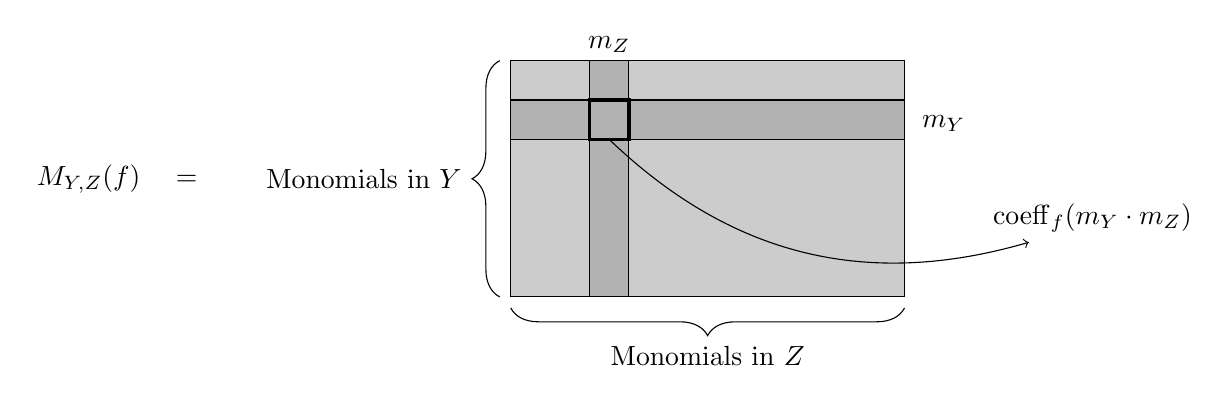
\begin{tikzpicture}
\node at (-5,1.5) {$M_{Y,Z}(f) \quad= $};
\draw[fill=black!20] (0,0) rectangle (5,3);

\draw[decorate,decoration={brace,amplitude=10pt,raise=4pt},yshift=0pt]
(0,0) -- (0,3);
\node[anchor=east] at (-0.5,1.5) {Monomials in $Y$};
\draw[decorate,decoration={brace,amplitude=10pt,mirror, raise=4pt},yshift=0pt] 
(0,0) -- (5,0);
\node[anchor=north] at (2.5,-0.5) {Monomials in $Z$};

\draw[fill=black!30] (1,0) rectangle (1.5,3);
\node at (1.25,3.2) {$m_Z$};

\draw[fill=black!30] (0,2) rectangle (5,2.5);
\node at (5.5,2.2) {$m_Y$};

\draw[very thick] (1,2) rectangle (1.5,2.5);

\node[anchor=west] at (6,1) {$\mathrm{coeff}_f(m_Y \cdot m_Z)$}
edge[<-,bend left] (1.25,2);
\end{tikzpicture}

\medskip

\noindent
The following observation is a an easy exercise. 

\begin{lemma}
Suppose a polynomial $f$ is can be computed as an entry in a product of $w\times w$ univariates matrices in the order $(x_1,\cdots, x_n)$, that is
\[
f \spaced{=} \inparen{A_1(x_1) \cdots A_n(x_n) }_{(1,1)}.
\]
Then, for every $i \in [n]$, for the partition $Y = \set{x_1, \ldots , x_{i}}$ and $Z = X \setminus Y$ we have $\rank(M_{Y,Z}(f)) \leq w$. 

Furthermore, the converse also holds. 
\end{lemma}

Hence, the rank of the partial derivative matrix can be used to prove lower bounds for ROABPs. \\

\begin{exercise}\label{ex:pdm-rank}
What is the rank of the partial derivative matrices for the following polynomials? 
\begin{itemize}
\item The elementary symmetric polynomials $\ESym_d$, under any partition.
\item Any $\SES$ circuit of size $s$, under any partition.
\item $\Det_n$ and $\Perm_n$ under the partition $X = Y \sqcup Z$ where $Y$ the variables from the first $n/2$ rows. 
\item The polynomial $(x_1 + x_2) \cdots (x_{2n-1} + x_{2n})$ under the partition $X = Y \sqcup Z$ with $Y = \set{x_1,\cdots, x_n}$. 
\item The polynomial $(x_1 + x_2) \cdots (x_{2n-1} + x_{2n})$ under the partition $X = Y \sqcup Z$ with $Y = \set{x_1,x_3,x_5,\cdots, x_{2n-1}}$. 
\end{itemize}
\end{exercise}

\subsection{An evaluation perspective}

For this section, let us assume that we are working with a field that is large enough. The following is an alternative way to study the rank of the partial derivative matrix under some partition. It is essentially the same, but sometimes is easier to reason with and we shall see a few examples in this chapter. 

\begin{definition}[Evaluation dimension]
Let $X = Y \sqcup Z$. The evaluation dimension of a polynomial $f$, with respect to $Y \sqcup Z$, denoted by $\evalDim_{Y,Z}(f)$,  is defined as the rank of the following polynomials
\[
\evalDim_{Y,Z}(f) \spaced{=} \rank\inparen{\setdef{f(\veca, Z) \in \F[Z]}{\veca \in \F^{|Y|}}}. 
\]
In other words, $\evalDim_{Y,Z}(f)$ of the space of partial evaluations of $f$ by setting $Y$ to arbitrary field constants. 
\end{definition}

\noindent 
The following lemma is easy to verify.

\begin{lemma}\label{lem:evalDim-to-coeffDim}
Over any field $\F$, we always have that $\evalDim_{Y,Z}(f) \leq \rank(M_{Y,Z}(f))$. If $|\F| \geq \deg(f)$, then
\[
\evalDim_{Y,Z}(f) \spaced{=} \rank(M_{Y,Z}(f)).
\]
\end{lemma}

To illustrate why this perspective is convenient, we shall take one example from \autoref{ex:pdm-rank} and compute the evaluation dimension of a $\SES$ circuit. 

\begin{claim}
Let $f = \sum_{i=1}^s \ell_i^d$. Then under any partition $X = Y \sqcup Z$, we have that $\evalDim_{Y,Z}(f) \leq (d+1) \cdot s$. 
\end{claim}
\begin{proof}
  It suffices to prove that the evaluation dimension of a single $\ell^d$ is at most $(d+1)$ and the lemma would follow due to sub-additivity.
Say $\ell = (a_0 + a_1 x_1 + \cdots + a_nx_n)$.
For any partition $X = Y \sqcup Z$, let $\ell_Y = \sum_{i\in Y} a_i x_i$ and $\ell_Z = \ell - \ell_Y$ so that $\ell = \ell_Y + \ell_Z$. Now if we take a partial evaluation of the $Y$ variables to field constants, the resulting polynomial is 
\[
(\alpha + \ell_Z)^d \spaced{=} \alpha^d \;+\; \alpha^{d-1} \binom{d}{1} \ell_Z \;+\; \cdots \;+\; \ell_Z^d. 
\]
And as we change the evaluation, the only change in the above equation is the value of $\alpha$. Hence it is clear that the rank of this space of polynomials is no more than $(d+1)$ as it is spanned by 
\[
\set{1, \ell_Z, \cdots, \ell_Z^d}.\qedhere
\]
\end{proof}

\begin{exercise}
Repeat \autoref{ex:pdm-rank} with evaluation dimension. 
\end{exercise}

\begin{exercise}
Suppose you have a degree $d$ polynomial $f$ so that $\dim{\partial^{\leq d}(f)}$ is at most $r$, that is, there are at most $r$ linearly independent partial derivatives of $f$. What can you say about $\evalDim_{Y,Z}(f)$ under any partition? 

What about the converse?
\end{exercise}

\bigskip 

The notion of partial derivative matrix is very useful and in the next chapter we shall see how it can be used to prove lower bounds for multilinear models.

%%% Local Variables: 
%%% mode: latex
%%% TeX-master: "fancymain"
%%% End: 


\chapter{Lower bounds for multilinear models}\label{chap:multilinear}

Most of the polynomials that are studied usually, like those described in Chapter~\ref{chap:notation}, are multilinear. A natural question is whether or not multilinear polynomials can be computed in a ``multilinear fashion''. This is formalized by what the model of multilinear circuits, in a way analogous to homogeneous circuits. 

\begin{definition}[Multilinear circuits]
A circuit $C$ is said to be \emph{multilinear} if every gate of the circuit computes a multilinear polynomial. A circuit is said to be \emph{syntactically multilinear} if for any $g = g_1 \times g_2$, there is no variable that has a path to both $g_1$ and $g_2$. 
\end{definition}

Note that syntactic multilinearity of course implies multilinearity as the definition forces all gates to compute multilinear polynomials. However, we could have a setting where there is a gate $g = g_1 \times g_2$ where some variable $x$ has a path to both $g_1$ and $g_2$ but it so turns out that $g_1$ is independent of $x$ due to other cancellations. However, for arithmetic formulas, the two notions are equivalent. 

\begin{exercise}
Given any arithmetic formula $\Phi$ that is multilinear, show that it can be converted to a formula $\Phi'$ of size $\poly(\Phi)$ that is syntactically multilinear. 
\end{exercise}

This section shall deal mainly with multilinear formulas so we may assume without loss of generality that they are syntactically multilinear. Raz \cite{raz2004} showed that multilinear formulas computing the $\Det_n$ or $\Perm_n$ must be of size $n^{\Omega(\log n)}$. The complexity measure used by Raz also led to exponential lower bounds for constant depth multilinear circuits \cite{raz-yehudayoff} and super-linear lower bounds for syntactic multilinear circuits \cite{RSY08}. We shall first give some intuition behind the complexity measure before actually seeing the lower bounds. 

\section{The partial derivative matrix}
\subsection*{Intuition}

A natural first step is to try the simpler task of proving lower bounds for depth-$3$ multilinear circuits. 
$$
f \quad = \ell_{11} \dots \ell_{1d} + \dots + \ell_{s1}\dots \ell_{sd}
$$
The task is now to construct a measure $\Gamma$ such that $\Gamma(\ell_1\dots \ell_d)$ is small whenever each $\ell_i$ is a linear polynomial and different $\ell_i$'s are over disjoint sets of variables. Consider the simplest case of $f = (a_1  + b_1x)(a_2  + b_2y)$. An observation is that the coefficients of $f$ are given by the $2\times 2$ matrix obtained as $[a_1\ b_1]^T [a_2\ b_2] = \insquare{\begin{array}{cc} a_1a_2 & a_1b_2\\ a_2 b_1 & b_1 b_2\end{array}}$. In other words, a polynomial $f = a_0 + a_1x + a_2y + a_3xy$ factorizes into two variable disjoint factors if and only if the matrix $\insquare{\begin{array}{cc} a_0 & a_1\\ a_2 & a_3\end{array}}$ has rank $1$. A straight-forward generalization of this to multiple variables yields the \emph{partial derivative matrix} (which was first introduced by Nisan \cite{nis91} in the context of non-commutative ABPs)\\

\begin{definition}
For any given partition of variables $X = Y \sqcup Z$, define the \emph{partial derivative matrix} $M_{Y,Z}(f)$ to be the matrix described as follows --- the rows are indexed by monomials in $Y$, columns indexed by monomials in $Z$, and the $(i,j)$-th entry of the matrix is the coefficient of the monomial $m_i(Y)\cdot m_j(Z)$ in $f$. We shall use $\Gamma^{\mathrm{[Raz]}}_{Y,Z}(f)$ to denote $\mathrm{rank}(M_{Y,Z}(f))$. Further, we shall call a polynomial $f$ to be \emph{full-rank} if $M_{Y,Z}(f)$ is full-rank.
\end{definition}

Here are some basic properties of the partial derivative matrix which would be extremely useful in later calculations.

\begin{observation}[Sub-additivity]\label{obs:pdm-subadditivity}
	For any partition $X = Y \sqcup Z$ and any pair of multilinear 
	polynomials $f$ and $g$ in $\FF[X]$ we have 
$\CM{Raz}_{Y,Z}(f+g) \spaced{\leq} \CM{Raz}_{Y,Z}(f) \spaced{+} \CM{Raz}_{Y,Z}(g)$.
\end{observation}
\begin{proof}
Follows from the linearity of the matrix. 
\end{proof}

\begin{observation}[Multiplicativity]\label{obs:pdm-multiplicativity}
If $f_1 \in \F[Y_1,Z_1]$ and $f_2 \in \F[Y_2, Z_2]$ with $Y = Y_1 \sqcup Y_2$ and $Z = Z_1 \sqcup Z_2$, then
$$
\CM{Raz}_{Y,Z}(f_1\cdot f_2) \spaced{=} \CM{Raz}_{Y_1, Z_1}(f_1) \spaced{\cdot} \CM{Raz}_{Y_2, Z_2}(f_2).
$$
\end{observation}
\begin{proof}
  It is not hard to see that $M_{Y,Z}(f_1\cdot f_2)$ is the tensor product $M_{Y_1, Z_1}(f_1) \otimes M_{Y_2, Z_2}(f_2)$, and the rank of a tensor product of two matrices is the product of the ranks.
\end{proof}

\begin{observation}\label{obs:pdm-upperbound}
  $\CM{Raz}_{Y,Z}(f) \spaced{\leq} 2^{\min(\abs{Y}, \abs{Z})}$.
\end{observation}
\begin{proof}
  The number of rows is $2^{\abs{Y}}$ and number of columns is $2^{\abs{Z}}$, and hence the rank is upper-bounded by the minimum.
\end{proof}


Let us get back to lower bounds for multilinear models, and attempt to use $\CM{Raz}_{Y,Z}(f)$ defined above. Unfortunately, there are examples of simple polynomials like $f = (y_1 + z_1)\dots (y_n + z_n)$ with $\CM{Raz}_{Y,Z}(f) = 2^n$. Raz's idea here was to look at $\CM{Raz}_{Y,Z}(f)$ for a \emph{random partition}, and show that with high probability the rank of the partial derivative matrix is far from full. As a toy example, we shall see why this has the potential to give lower bounds for depth-$3$ multilinear circuits. 

\begin{lemma}
Let $f(X) = \ell_1 \dots \ell_d$ be an $n$-variate multilinear polynomial. If $X = Y\sqcup Z$ is a random partition with $|Y| = |Z| = |X|/2$, then with high probability we have
$$
\CM{Raz}_{Y,Z}(f) \quad \leq \quad 2^{|X|/2} \cdot 2^{-|X|/16}.
$$
\end{lemma}

It is to be noted that we should expect a random polynomial to be full-rank with respect to any partition, so the measure $\CM{Raz}_{Y,Z}(f)$ is expected to be $2^{|X|/2}$ which should yield a lower bound of $2^{\Omega(|X|)}$. 

\begin{proof-sketch}
Without loss of generality we can assume that each $\ell_i$ depends on at least two variables as removing the $\ell_i$'s that depend on just one variable does not alter $\CM{Raz}_{Y,Z}(f)$ with respect to any partition. Let $|X| = n$. 

Using Observation~\ref{obs:pdm-multiplicativity}, $\CM{Raz}_{Y,Z}(f) \leq 2^d$ and hence if $d < n/3$ then we are done. Hence assume that $d \geq n/3$. By a simple averaging argument, there must hence be at least $d/4$ of the $\ell_i$'s that depend on at most $3$ variables; we shall refer to these as the \emph{small} $\ell_i$'s. 

Since the partition is chosen at random, on expectation a quarter of the small $\ell_i$'s would have all its variables mapped to either $Y$ or $Z$, hence not contributing to $\CM{Raz}_{Y,Z}(f)$. Therefore, with high probability,
$$
\CM{Raz}_{Y,Z}(f) \quad \leq \quad 2^{d} \cdot 2^{-d/16} \spaced{\leq} 2^{n/2} \cdot 2^{-n/16}.
$$
\end{proof-sketch}

More generally, if $f = g_1(X_1)\dots g_t(X_t)$ where the $X_i$'s are mutually disjoint, then a random partition is very unlikely to partition all the $X_i$'s into almost equal parts. This shall be formalized in the next section to prove the lower bound for multilinear formulas. 

\section{Lower bound for multilinear formulas}
	We now present the lower bound for multilinear formulas due 
	to \cite{raz2004}. The first step of our roadmap is to find 
	a suitable normal form for multilinear formulas. The normal 
	form that we use is from the survey by Shpilka and 
	Yehudayoff \cite{sy}. 	

\subsection{Formulas to log-product sums}

The following structural lemma shows that any multilinear formula can be converted in to a small sum of \emph{log-product} polynomials. The techniques of the following lemma can also be used in other settings with minor modifications, and we shall encounter a different version of this lemma later as well.

\begin{definition}\label{defn:mult-logproduct}
  A multilinear polynomial $f\in \F[X]$ is called a \emph{multilinear log-product} polynomial if $f = g_1\dots g_t$ and there exists a partition of variables $X = X_1 \sqcup \dots \sqcup X_t$ such that
  \begin{itemize}
  \item $g_i \in \F[X_i]$ for all $i \in [t]$.
  \item $\frac{|X|}{3^i} \leq |X_i| \leq \frac{2|X|}{3^i}$ for all
    $i$, and $|X_t| = 1$.
  \end{itemize}
\end{definition}

\begin{lemma}\label{lem:mult-logproduct}
  Let $\Phi$ be a multilinear formula of size $s$ computing a polynomial $p$. Then $f$ can be written as a sum of $(s+1)$ log-product multivariate polynomials.
\end{lemma}
\begin{proof}
  Similar to Lemma~\ref{lem:formula-depth-reduction}, let $v$ be a node in $\Phi$ such that set of variables $X_v$ that it depends on satisfies $\frac{|X|}{3} \leq \abs{X_v} \leq \frac{2|X|}{3}$. If $\Phi_v$ is the polynomial computed at this node, then $f$ can be written as
  $$
  f \spaced{=} \Phi_v \cdot g_1 + \Phi_{v=0} \quad\text{for some $g_1 \in \F[X\setminus X_v]$}.
  $$
  where $\Phi_{v=0}$ is the formula obtained by replacing the node $v$ by zero. Note that the subtree at the node $v$ is completely disjoint from $\Phi_{v=0}$. Hence the sum of the sizes of $\Phi_v$ and $\Phi_{v=0}$ is at most $s$. Hence, $g_1 \in \F[X\setminus X_v]$ and $\frac{|X|}{3} \leq \abs{X \setminus X_v} \leq \frac{2|X|}{3}$. Inducting on the formulas $\Phi_v$ and $\Phi_{v=0}$ gives the lemma.
\end{proof}

\subsection{Log-products are far from full-rank on a random
  partition}

The main technical part of the proof is to show that log-product multivariate polynomials are far from full-rank under a random partition of variables. This would let us show that a sum of log-product multivariate polynomials cannot be full rank unless it is a very large sum.\\

{\bf Main idea: } Suppose $f = g_1 \dots g_t$ where each $g_i \in \F[X_i]$. Let $X = Y \sqcup Z$ be a random partition with $|Y| = |Z| = |X|/2$, and $Y_i = Y \intersection X_i$ and $Z_i = Z \intersection X_i$. Let $d_i = \abs{\frac{|Y_i| - |Z_i|}{2}}$ measure the imbalance between the sizes of $Y_i$ and $Z_i$, and we shall say $X_i$ is $k$-imbalanced if $d_i \geq k$. Let $b_i = \frac{|Y_i| + |Z_i|}{2} = \frac{|X_i|}{2}$.

By Observation~\ref{obs:pdm-multiplicativity}, we know that 
\begin{eqnarray*}
\CM{Raz}_{Y,Z}(f) & = & \CM{Raz}_{Y_i,Z_i}(g_1) \dots \CM{Raz}_{Y_i,Z_i}(g_t)\\
 & \leq & 2^{\min(|Y_1|,|Z_1|)} \cdots  \cdot 2^{\min(|Y_t|,|Z_t|)}\\ 
 & = & 2^{b_1  - d_1} \cdots 2^{b_t - d_t} = \frac{2^{|X|/2}}{2^{d_1 + \dots + d_t}}.
\end{eqnarray*}

Hence, even if one of the $X_i$'s is a little imbalanced, then the product is far from full-rank. \\

Lemma~\ref{lem:mult-logproduct} shows that the size of $X_i$ decreases slowly with $i$, and it is not hard to show that $\abs{X_i} \geq \sqrt{\abs{X}}$ for $i \leq t'\eqdef\frac{\log{\abs{X}}}{100}$. We wish to show that the probability that none of $g_i$ (for $i\leq t'$) is $k$-unbalanced for $k = \abs{X}^{1/20}$ is very small. Let $\mathcal{E}_i$ be the event that $X_i$ is not $k$-unbalanced. The goal is to upper bound the probability that all the events $\mathcal{E}_i$ hold. These probability calculations would follow from this lemma about the \emph{hypergeometric distribution}.\\

{\bf Hypergeometric Distribution: } Fix parameters $n, g, r \geq 0$, and let $G \subseteq [n]$ with $|G| = g$. Informally, the hypergeometric distribution is the distribution obtained on the intersection sizes of a random set of size $r$ with a fixed set of size $g$ from a universe of size $n$. 
Formally, the random variable $\mathcal{H}(n,g,r)$ is defined as:
$$
\Pr\insquare{\mathcal{H}(n,g,r) = k} \spaced{=} \Pr_{R\subseteq [n],|R| = r}\insquare{\abs{R \intersection G} = k} = \frac{\binom{g}{k}\binom{n-g}{r-k}}{\binom{n}{r}}.
$$


The following lemma shows that for a fairly large range of parameters, the hypergeometric distribution does not put too much mass on any value.

\begin{lemma}\label{lem:hypergeom_low-weight}
  Let $n,g,r$ be parameters such that $\frac{n}{4} \leq r \leq \frac{3n}{4}$ and $0\leq g\leq \frac{2n}{3}$. Then for any $t\leq g$,
  $$
  \Pr\insquare{\mathcal{H}(n,g,r) = t} \spaced{\leq} O\inparen{\frac{1}{\sqrt{g}}}.
  $$
\end{lemma}
The proof of this lemma follows from standard binomial coefficient estimates on the probability.\\

Let us go back to estimating the probability that all the events $\mathcal{E}_i$ hold.
\begin{eqnarray*}
  \Pr\insquare{\mathcal{E}_1 \wedge \dots \wedge \mathcal{E}_{t'}} & = & \Pr[\mathcal{E}_1] \cdot \Pr[\mathcal{E}_2 \mid \mathcal{E}_1] \cdots \Pr[\mathcal{E}_{t'}\mid \mathcal{E}_1 \wedge \dots \wedge \mathcal{E}_{t'-1}].
\end{eqnarray*}
The event $\mathcal{E}_1$ is just the probability that a random set $Y$ of size $|X|/2$ intersects $X_1$ in $t$ places where $t \in \insquare{\frac{|X_i|}{2} -k , \frac{|X_i|}{2} -k}$. This is just a particular setting of the hypergeometric distribution and Lemma~\ref{lem:hypergeom_low-weight} asserts that
$$
\Pr[\mathcal{E}_1] \spaced{\leq} O\inparen{\frac{2k}{\sqrt{|X|}}}.
$$
To apply a similar bound for the other terms, consider the event $\mathcal{E}_i$ given that $\mathcal{E}_1, \dots, \mathcal{E}_{i-1}$ hold. Let $X' = X \setminus (X_1 \union \dots \union X_{i-1})$ and $Y' = Y\intersection X'$. The fact that $\mathcal{E}_1,\dots, \mathcal{E}_{i-1}$ hold means that the partition has been fairly balanced in the first $(i-1)$ parts and hence $|Y'| \leq |X'| + ik$. Hence, we would still be in the range of parameters in Lemma~\ref{lem:hypergeom_low-weight} to also get that
\begin{eqnarray*}
  \forall i\leq t'\quad \Pr[\mathcal{E}_i\mid \mathcal{E}_1 \wedge \cdots \wedge \mathcal{E}_{i-1}] &\leq& O\inparen{\frac{2k}{\sqrt{|X|}}}\\
  \implies \Pr\insquare{\mathcal{E}_1\wedge \dots \wedge \mathcal{E}_{t'}} & \leq & \abs{X}^{-\epsilon \log \abs{X}} \quad\text{for some $\epsilon > 0$}  \\
  \implies \Pr\insquare{\CM{Raz}_{Y,Z}(g_1\dots g_t) \leq 2^{(|X|/2) - |X|^{1/20}}} & \leq & \abs{X}^{-\epsilon \log \abs{X}}.
\end{eqnarray*}

\begin{sloppy}
	Hence, if $g_1\dots g_t$ is a log-product multilinear polynomial, 
	then with probability at least $\inparen{1 - |X|^{-\epsilon \log |X|}}$ 
	we have that $\CM{Raz}_{Y,Z}(g_1\dots g_t) \leq 2^{(|X|/2) - |X|^{1/20}}$. 
	Further, if $f$ is computable by a multilinear formula of size $s$ then, 
	by Lemma~\ref{lem:mult-logproduct}, $f$ can be written as a sum of 
	$(s+1)$ log-product multilinear polynomials. Hence, with probability 
	at least $\inparen{1 - (s+1)|X|^{-\epsilon \log |X|}}$ we have that
		$$\CM{Raz}_{Y,Z}(f) \spaced{\leq} (s+1) \cdot 2^{(|X|/2) - |X|^{1/20}}. $$
	Hence, if $(s+1) < |X|^{(\epsilon/2) \log |X|}$, then with high 
	probability a random partition would ensure 
	$\CM{Raz}_{Y,Z}(f) \ll 2^{|X|/2}$. Let us record this as a lemma.
\end{sloppy}

\begin{lemma}\label{lem:multformula-lowrank}
  Let $f \in \F[X]$ be computed by a multilinear formula of size $s < |X|^{(\epsilon/2) \log |X|}$ for a small enough constant $\epsilon > 0$. Then with probability at least $(1 - |X|^{-(\epsilon/2)\log |X|})$ we have $$\CM{Raz}_{Y,Z}(f) \spaced{\leq} (s+1)\cdot 2^{|X|/2} \cdot 2^{-|X|^{1/20}}$$ for a random partition $X = Y \sqcup Z$ with $|Y| = |Z| = |X|/2$.
\end{lemma}

\subsection{$\Det_n$ and $\Perm_n$ have large rank}

The last step of the proof would be to find an explicit polynomial whose partial derivative matrix under a random partition has large rank. As earlier, our candidate polynomial would be $\Det_n$ or $\Perm_n$. Unfortunately, both these polynomials are over $n^2$ variables and degree $n$. It is not hard to verify that the rank of the partial derivative matrix of $\Det_n$ or $\Perm_n$ can never be greater than $2^{2n}$. Hence directly using Lemma~\ref{lem:multformula-lowrank}, we would have $2^{O(n)}$ competing with $2^{n^2/2 - n^{O(1)}}$ which is simply futile. A simple fix is to first randomly restrict ourselves to fewer variables and then apply Lemma~\ref{lem:multformula-lowrank}. 

Let $m = n^{1/3}$. Let $\sigma$ be a random restriction that assigns random values to all but $2m$ randomly chosen variables. We shall call this set of $2m$ variables as $X$, and randomly partition this into two sets $Y$ and $Z$ of size $m$ each. Hence, $\sigma(\Det_n)$ reduces to a multilinear polynomial over $2m$ variables. It is also worth noting that a multilinear formula remains a multilinear formula under this restriction. The following claim is easy to verify. 

\begin{claim}
With probability at least $1/2$, the variables in $X$ belong to distinct rows and columns. 
\end{claim}

We shall restrict ourselves to only these random restrictions, and without loss of generality let the sets be $Y = \inbrace{x_{1,1},x_{3,3},\dots,x_{2m-1,2m-1}}$ and $Z = \inbrace{x_{2,2},x_{4,4},\dots, x_{2m,2m}}$. For ease of notation, we shall refer to $x_{2i-1,2i-1}$ as $y_i$ and $x_{2i,2i}$ as $z_i$ for $i = 1,\dots, m$. 

Consider the following restriction:
\begin{eqnarray*}
f & = & \Det \insquare{ \begin{array}{cccccccc}
y_1 & 1   &        &     &     &  &        &   \\
1   & z_1 &        &     &     &  &        &   \\
    &     & \ddots &     &     &  &        &   \\
    &     &        & y_m &1    &  &        &   \\
    &     &        & 1   &z_m  &  &        &   \\
    &     &        &     &     & 1&        &   \\
    &     &        &     &     &  & \ddots &   \\
    &     &        &     &     &  &        & 1
  \end{array}}\\
 &= & (y_1z_1 - 1)\dots (y_mz_m - 1).
\end{eqnarray*}
It is easy to check that $\CM{Raz}_{Y,Z}(f) = 2^m$. Although this is a single restriction with large rank, the Schwartz-Zippel-DeMillo-Lipton lemma immediately gives that random restriction would also have rank $2^m$ with high probability\footnote{provided the underlying field is large, but this isn't really a concern as we can work with a large enough extension if necessary}. We shall record this as a lemma. 

\begin{lemma}\label{lem:det-raz-lowerbound}
With probability at least $1/100$, we have that $\CM{Raz}_{Y,Z}(\sigma(\Det_n)) = 2^m$ where $\sigma$ is a random restriction to $2m$ variables for $m = n^{1/3}$. 
\end{lemma}


Combining Lemma~\ref{lem:det-raz-lowerbound} with Lemma~\ref{lem:multformula-lowrank}, we have the following theorem. 

\begin{theorem}[\cite{raz2004}] Any multilinear formula computing $\Det_n$ or $\Perm_n$ must be of size $n^{\Omega(\log n)}$. \qed
\end{theorem}


\section{Stronger lower bounds for constant depth multilinear formulas}

Looking back at Lemma~\ref{lem:multformula-lowrank}, we see that whenever $f(X)$ is computable by a size $s$ multilinear formula $\CM{Raz}_{Y,Z}(f)$ is exponentially smaller than $2^{|X|/2}$ with probability $\inparen{1 - s\cdot |X|^{-\epsilon \log |X|}}$. Hence we had to settle for a $n^{\Omega(\log n)}$ lower bound not because of the rank deficit but rather because of the bounds in the probability estimate. Unfortunately, this lower bound technique cannot yield a better lower bound for multilinear formulas as there are explicit examples of polynomials computable by poly-sized multilinear circuits with $\CM{Raz}_{Y,Z}(f) = 2^{|X|/2}$ under \emph{every} partition \cite{Raz06}. However, the probability bound can be improved in the case of constant depth multilinear circuits to give stronger lower bounds. 


Note that Lemma~\ref{lem:multformula-lowrank} was proved by considering \emph{multilinear log-products} (Definition~\ref{defn:mult-logproduct}) as the building blocks. To show that a multilinear log product $g_1(X_1)\dots g_{\ell}(X_\ell)$ has small rank under a random partition, we argued that the probability that all the $X_i$'s are partitioned in a roughly balanced fashion is quite small. This was essentially done by thinking of this as $\ell = O(\log n)$ close-to-independent events, each with probability $1/\mathrm{poly}(n)$. 

If $\ell$ was much larger than $\log n$ (with other parameters being roughly the same), it should be intuitively natural to expect a much lower probability of all the $X_i$'s being partitioned in a roughly balanced manner. This indeed is the case for constant depth multilinear circuits, and we briefly sketch the key points where they differ from the earlier proof. The first is an analogue of Definition~\ref{defn:mult-logproduct} in this setting. 

\begin{definition}\label{defn:mult-t-prod}
A multilinear polynomial $f$ is said to be a \emph{multilinear $t$-product} if $f$ can be written as $f = g_1\dots g_t$ with the following properties:
\begin{itemize}
\item The variable sets of the $g_i$ are mutually disjoint
\item Each $g_i$ non-trivially depends on at least $t$ variables
\end{itemize}
\end{definition}

\begin{lemma}\label{lem:mult-t-prod-rep}
Let $f$ be a multilinear polynomial of degree $d$ over $n$ variables that is computed by a depth-$\Delta$ multilinear formula $\Phi$ of size $s$. Then, $f$ can be written as a sum of at most $s$ multilinear $t$-products for $t = \inparen{n/100}^{1/2\Delta}$, and a multilinear polynomial of degree at most $n/100$.  
\end{lemma}
\begin{proof}
If $d < n/100$, then the lemma is vacuously true. Since $\Phi$ is a formula of depth $\Delta$ and computes a polynomial of degree $d > n/100$, there must be at least one product gate $v$ of fan-in at least $\inparen{\frac{n}{100}}^{1/\Delta} = t^2$. Then similar to Lemma~\ref{lem:mult-logproduct}, 
$$
f \quad=\quad \Phi_v \cdot f'  + \Phi_{v=0}
$$
As $\Phi_v$ is a product of $t^2$ polynomials, by grouping the factors together we have that $\Phi_v \cdot f'$ is a multilinear $t$-product. Further, $\Phi_{v=0}$ is a multilinear polynomial that is computable by a depth-$\Delta$ formula of smaller size and we can induct on $\Phi_{v=0}$. 
\end{proof}

\begin{lemma}\label{lem:mult-const-depth-upper-bound}
Let $f(X)$ be an $n$-variate polynomial computed by a depth-$\Delta$ multilinear formula of size $s$. If $X = Y \sqcup Z$ is a randomly chosen partition with $|Y| = |Z| = n/2$, then with probability at least $(1 - s \cdot \exp({-n^{\Omega(1/\Delta)}}))$ we have
$$
\CM{Raz}_{Y,Z}(f) \quad\leq\quad (s+1) \cdot 2^{n/2} \cdot \exp(-n^{\Omega(1/\Delta)}).
$$
\end{lemma}
\begin{proof-sketch}
By Lemma~\ref{lem:mult-t-prod-rep}, we have that $f$ can be written as $g_0 + g_1 + \dots + g_s$ where $\deg(g_0) \leq n/100$ and $g_1,\dots, g_s$ are multilinear $t$-products. Note that since $g_0$ is a multilinear polynomial of degree at most $(n/100)$, the number of monomials in $g_0$ is at most $\binom{n}{n/100} \leq 2^{n/10}$. Hence, $\CM{Raz}_{Y,Z}(g_0) \leq 2^{n/10}$. 

For the other $g_i$'s, we can bound the probability that $\CM{Raz}_{Y,Z}(g_i)$ is large in a very similar fashion as in Lemma~\ref{lem:multformula-lowrank}, as the probability that all the factors of $g_i$ are partitioned in a balanced manner is roughly the intersection of $t$ independent events. By very similar estimates, this probability can be bounded by $(1/\mathrm{poly}(n))^t$. Hence, with high probability 
$$
\CM{Raz}_{Y,Z}(f) \spaced{\leq} \CM{Raz}_{Y,Z}(g_0) + \dots + \CM{Raz}_{Y,Z}(g_s) \spaced{\leq} (s+1)\cdot 2^{n/2} \cdot \exp(-n^{\Omega(1/\Delta)}).
$$
\end{proof-sketch}

Combining Lemma~\ref{lem:mult-const-depth-upper-bound} with Lemma~\ref{lem:det-raz-lowerbound}, we have the following theorem of Raz and Yehudayoff. 

\begin{theorem}[\cite{raz-yehudayoff}]
Any multilinear formula of depth $\Delta$ computing $\Det_n$ or $\Perm_n$ must be of size $\exp(n^{\Omega(1/\Delta)})$.  \qed
\end{theorem}



%%% Local Variables: 
%%% mode: latex
%%% TeX-master: "main"
%%% End: 


\chapter{Tensor rank and formula lower bounds}\label{chap:tensorrk}

In this chapter, we will establish an apriori surprising connection between lower bounds for homogeneous arithmetic formula and constructing explicit tensors of full rank.
The chapter is based on a result of Raz~\cite{raz10}.

\section{Tensors}

Tensors are natural \emph{higher dimensional} analogues of matrices.
A matrices is nothing but a two dimensional array filled in with numbers from some underlying field.
A tensor is a higher dimensional version of this, where we have an $d$-dimensional cuboid filled with numbers.
A tensor $T$ is a map of the form
\[
T: [m_1] \times \cdots \times [m_d] \longrightarrow \F
\]
the same way an $m\times n$ matrix a map from $[m] \times [n] \rightarrow \F$.
However, if one wants to understand a tensor more functionally (similarly to how it is useful to think of matrices as linear transformations on vector spaces), it is more natural to extend this definition linearly as follows.

\begin{definition}[Tensor]\label{defn:tensor}
A tensor $T$ is a map of the form 
\[
T: V_1 \times \cdots \times V_d \longrightarrow \F
\]
where each $V_i$ is a vector space over $\F$, of say dimension $m_i$, which is linear in every coordinate i.e.
\[
T(\vecv_1, \ldots,\alpha\vecv_i + \beta\vecv_i', \ldots, \vecv_d) = \alpha T(\vecv_1, \ldots,\vecv_i, \ldots, \vecv_d) + \beta T(\vecv_1, \ldots,\vecv_i', \ldots, \vecv_d).
\]
The parameter $r$ is called the \emph{order} of the tensor, and we say that the \emph{shape of $T$} is $m_1 \times \cdots \times m_d$. 
\end{definition}
Since a tensor is linear in every coordinate, it suffices to specify the image of $T$ at the basis of $V_1 \times \cdots \times V_d$ and extend it linearly.
So a tensor can indeed be thought of as filling up a $d$-dimensional array of shape $[m_1]\times \cdots \times [m_d]$ by field elements, the same way an $m\times n$ matrix is specified by an $m\times n$ array filled up with field elements.
Indeed, a matrix is nothing but an order-$2$ tensor.

It would sometimes be useful to switch between the two notions of thinking of a tensor as a multilinear map from $V_1 \times \cdots \times V_d$ to $\F$ and thinking a tensor as just a map from $[m_1] \times \cdots \times [m_d]$.
So throughout this chapter, we shall fix a basis $\set{\vece_{i1},\ldots, \vece_{im_i}}$ for $V_i$ and when we shall use $T[j_1,\ldots, j_d]$ to really denote $T(\vece_{1j_1},\ldots, \vece_{dj_d})$.

\subsection{Tensors as polynomials}

In our setting, it would be useful to think of tensors as a restricted form of multilinear polynomials that are called \emph{set-multilinear polynomials}.

\begin{definition}[Set-multilinear polynomials]\label{defn:set-multilinear}
  Let $\vecx = \vecx_1 \sqcup \cdots \sqcup \vecx_d$ be a partition of variables and let $|\vecx_i| = m_i$.
A polynomial $f(\vecx)$ is said to be \emph{set-multilinear} with respect to the above partition if every monomial $m$ in $f$ satisfies $\abs{m \intersection X_i} = 1$ for all $i \in [d]$.
\end{definition}
In other words, each monomial in $f$ picks up at most one variable from each part in the partition. It is easy to see that many natural polynomials such as $\Det$ or $\Perm$ or $\NW$ are all set-multilinear for an appropriate partition of variables. 

\begin{observation}\label{obs:tensor-to-sml}
  For any tensor $T$ of shape $[m_1] \times \cdots \times [m_d]$, we can associate a set-multilinear polynomial $f(\vecx)$ with $\vecx = \vecx_1 \sqcup \cdots \sqcup \vecx_d$ and $\vecx_i = \set{x_{i1}, \ldots, x_{im_i}}$ as
\begin{equation}\label{eqn:tensor-sml}
f(\vecx) \spaced{=} \sum_{\substack{1 \leq i_j \leq m_j\\ \forall j \in [d]}}  T(i_1,\ldots, i_d) \cdot x_{1i_1}\cdots x_{di_d}.
\end{equation}
\end{observation}

Another representation is to just use a single variable $x_j$ for a part $\vecx_j$ and use higher powers.
That way, we can associate the following polynomial with a tensor $T$:
\begin{equation}\label{eqn:tensor-to-prod-univariates}
f(x_1,\ldots, x_d) \spaced{=} \sum_{\substack{1 \leq i_j \leq m_j\\ \forall j \in [d]}}  T(i_1,\ldots, i_d) \cdot x_{1}^{i_1}\cdots x_{d}^{i_d}.
\end{equation}
The same also holds in the other direction where we can interpret any set-multilinear polynomial as an appropriate tensor. 


\subsection{Rank of a tensor}

Just like any matrix has a natural definition of \emph{rank}, there is an analogue for tensors as well.
The rank of a matrix $M$ can be defined as the smallest $r$ for which $M$ can be written as a sum of $r$ matrices of rank $1$.
A rank-$1$ matrix is just a matrix of the form $\vecu \vecv^T$ where the $(i,j)$-th entry is $u_iv_j$.
We shall abuse\footnote{it is abuse because it is really a tensor product of $\vecu$ and $\vecv^T$.}
notation and use $\vecu \otimes \vecv$ to denote the order-$2$ tensor $T$ where $T[i,j] = u_i v_j$.
This naturally generalizes to higher order as well.

\begin{definition}[Elementary tensors, and tensor rank]
  For $\vecv_1\in V_1, \ldots, \vecv_d \in V_d$, define the tensor $\vecv_1 \otimes \cdots \otimes \vecv_d$ to be the tensor $E$ given by
\[
E[j_1,\ldots, j_d] = (\vecv_1)_{j_1} \cdots (\vecv_d)_{j_d}.
\]
We shall call such tensors as \emph{elementary tensors} or \emph{rank-$1$ tensors}. 

For an arbitrary tensor $T$, the \emph{tensor rank of $T$}, denoted by $\rank(T)$, is the smallest $r$ such that $T$ can be expressed as a sum of $r$ elementary tensors. 
\end{definition}

\noindent 
What do elementary tensors look like as polynomials?
Let us consider the \emph{set-multilinear} polynomial setting as in \eqref{eqn:tensor-sml}.
It is easy to see that a rank-$1$ tensor is precisely a \emph{set-multilinear} product of linear forms such as
\[
f(\vecx) \spaced{=} \ell_1(\vecx_1) \cdots \ell_d(\vecx_d)
\]
where each $\ell_i(\vecx_i)$ is a linear form in the variables in $\vecx_i$. \\

In the setting of \eqref{eqn:tensor-to-prod-univariates}, it is easy to see that a rank-$1$ tensor is precisely a \emph{product of univariates} such as
\[
f(\vecx) \spaced{=} f_1(x_1)\cdots f_d(x_d).
\]
\noindent
Hence the following three questions are equivalent:
\begin{itemize}
\setlength\itemsep{0em}
\item Given a tensor $T$, find its rank. 
\item Given a set-multilinear polynomial $f$, find the smallest set-multilinear $\SPS$ circuit computing it. 
\item Given a polynomial $f$, find the smallest expression as a sum of product of univariates.
\end{itemize}

However, unlike matrices, computing the rank of even an order-$3$ tensor is $\NP$-hard \cite{h90}.
But one could still ask if we can prove good upper or lower bounds for some specific tensors, or try to find a tensor with large rank.
But before that, let us look at some basic properties that tensor rank satisfies.

\subsection*{Properties of  tensor rank}

The following are a couple of basic properties that follows almost immediately from the definitions.

\begin{lemma}[Sub-additivity of tensor rank]\label{lem:tensor-subadditivity}
  Let $T_1$ and $T_2$ be two tensors of the same shape and order.
Then, if $T = T_1 + T_2$, then $\rank(T) \leq \rank(T_1) + \rank(T_2)$.
\end{lemma}

\begin{lemma}[Sub-multiplicativity of tensor rank]\label{lem:tensor-submultiplicativity}
  Let $T_1: V_1 \times \cdots \times V_{d_1} \rightarrow \F$ and $T_2: W_1 \times \cdots \times W_{d_2} \rightarrow \F$ be two tensors.
Then if $T = T_1 \otimes T_2$ given by
\[
T[i_1,\ldots, i_{d_1},j_1,\ldots, j_{d_2}] = T_1[i_1,\ldots, i_{d_1}] \cdot T_2[j_1,\ldots, j_{d_2}],
\]
then $\rank(T) \leq \rank(T_1) \cdot \rank(T_2)$. 
\end{lemma}

\begin{exercise}
  Show that in fact $\rank(T_1 \otimes T_2) = \rank(T_1) \cdot \rank(T_2)$.
\end{exercise}

\subsection{Upper bounds on tensor rank}

Let us consider an order-$d$ tensor $T$ of shape $n \times \cdots \times n$.
How large can $\rank(T)$ be?
One possible upper bound we could say is $n^d$.
Surely, the tensor is an $d$-dimensional array with just $n^d$ entries.
We can certainly write it as a sum of $n^d$ elementary tensors of the form $\vece_{j_1} \otimes \cdots \otimes \vece_{j_d}$.
So clearly $\rank(T) \leq n^d$.
But we can do a little better.
Consider the case when $d=2$, and we have an $n\times n$ matrix.
The bound on the rank is not $n^2$ but rather $n$.
This indicates that one should be able to do a bit better than $n^d$ for the general case.
Indeed we can.

\begin{lemma}\label{lem:tensor-rank-trivial-upperbound}
  Let $T$ be an order-$d$ tensor of shape $n\times \cdots \times n$.
Then, $\rank(T) \leq n^{d-1}$.
\end{lemma}
\begin{proof}
  Let us revisit the case when $d=2$, where we know an $n\times n$ matrix has rank at most $n$.
Interpreting this statement via \eqref{eqn:tensor-to-prod-univariates}, this implies that of $q(x_1,x_2)$ is a bi-variate with degree in each variable bounded by $n$, then $q$ can be written as
\[
q(x_1,x_2) = \sum_{i=1}^n g_i(x_1) h_i(x_2).
\]
Therefore, if $f(x_1,\ldots, x_d)$ is a polynomial with degree in each variable bounded by $n$, then we can write $f$ as
\begin{align*}
f(x_1,\ldots, x_d) &= \sum_{m \in \mathrm{Mon}\set{x_3,\ldots, x_d}} m \cdot q_m(x_1,x_2)\\
& = \sum_{m \in \mathrm{Mon}\set{x_3,\ldots, x_d}} m \cdot \inparen{\sum_{i=1}^n g_{m,i}(x_1) \cdot h_{m,i}(x_2)}
\end{align*}
which is a sum of product of univariates of top fan-in $n \cdot n^{d-2} = n^{d-1}$. 
\end{proof}

A counting argument would say that there do exist tensors of rank at least $n^{d-1}/d$ as each elementary tensor has $nd$ \emph{degrees of freedom} and an arbitrary tensor has $n^d$ \emph{degrees of freedom}.
One might think that the above upper bound of $n^{d-1}$ should be tight.
Bizarrely, it is not!
For example (cf.
\cite{p85}), the maximum rank of any tensor of shape $2\times 2 \times 2$ is $3$ and not $4$ as one might expect!
Tensor rank also behaves in some strange ways under \emph{limits} unlike the usual matrix rank.
But a big open question is to find explicit tensors of such large rank.

\begin{openproblem}
Can we find an explicit tensor $T: [n]^d \rightarrow \F$ of rank $n^{d(1 - o(1))}$?
\end{openproblem}

Raz's \cite{raz10} showed that in certain regimes, an answer to the above question would yield arithmetic formula lower bounds. 

\section{Tensor rank of small formulas}

From this section onwards, we shall assume the \emph{set-multilinear polynomial} interpretation of a tensor $T:[n]^d \rightarrow \F$ as described in~\eqref{eqn:tensor-sml}.
Hence our variables $\vecx$ is partitioned as $\vecx = \vecx_1 \sqcup \cdots \sqcup \vecx_d$ with $\abs{\vecx_i} = n$ for all $i\in [d]$.
The main motivating question would be the following:
\begin{quote}
If $f$ is a set-multilinear polynomial that is computed by a small formula, what can one say about its tensor rank?
\end{quote}

To begin with, let us restrict ourselves to certain structured formulas that in a sense \emph{respects} the partition defined. 

\begin{definition}[Set-multilinear formulas] A formula $\Phi$ is said
  to be a \emph{set-multilinear formula} if for every gate in the formula computes a set-multilinear polynomial.
\end{definition}

From the above definition, note that the set-multilinear formulas are a subclass of homogeneous formulas.
As in the multilinear setting, it is easy to see that set-multilinearity for formulas can be made a \emph{syntactic} restriction where each gate computes a tensor, with addition gates only adding ``alike'' tensors and multiplication gates multiplying disjoint tensors.

\begin{exercise}
  Show that set-multilinear formulas can, without loss of generality, be assumed to be syntactically set-multilinear formulas.
\end{exercise}

\noindent
An easier question to the one above would be the following:

\begin{quote}
  If $f$ is a set-multilinear polynomial that is computed by a small \emph{set-multilinear} formula, what can one say about its tensor rank?
\end{quote}

In the rest of this chapter, we shall prove the following result of Raz \cite{raz10}. 

\begin{theorem}[\cite{raz10}] \label{thm:raz-tensorrank-sml} Let
  $\Phi$ be a set-multilinear formula of size $s \leq n^c$ computing a polynomial $f(\vecx_1,\ldots, \vecx_d)$.
Then,
\[
\rank(f) \spaced{\leq} \frac{n^d}{n^{d/\exp(c)}}. 
\] 
\end{theorem}

In the setting when $d$ is small, Raz \cite{raz10} also showed that formulas can be converted to set-multilinear formulas with a modest cost. 

\begin{theorem}[\cite{raz10}]\label{thm:form-to-smlform}
  Suppose $d = O\pfrac{\log n}{\log\log n}$.
If $\Phi$ is a formula of size $s = \poly(n)$ that computes a set-multilinear polynomial $f(\vecx_1,\ldots, \vecx_d)$, then there is a \emph{set-multilinear} formula of $\poly(s)$ size that computes $f$ as well.
\end{theorem}

As a corollary, finding explicit tensors of almost full rank would imply super-polynomial formula lower bounds in the low-degree regime.

\begin{corollary}[\cite{raz10}]
  If $f(\vecx_1,\ldots, \vecx_d)$ is an explicit tensor of rank $n^{d(1- o(1))}$ with $\omega(1) = d = O\pfrac{\log n}{\log\log n}$, then any formula computing $f$ must be of super-polynomial size.
\end{corollary}

The above two theorems are of very different flavours and should really be thought of as two independent surprising results.
\autoref{thm:raz-tensorrank-sml} is a tensor-rank upper bound and \autoref{thm:form-to-smlform} is a structural result.
We shall first address \autoref{thm:raz-tensorrank-sml} in the next section and address \autoref{thm:form-to-smlform} after that.

\subsection{The tensor-rank upper-bound}

We shall now prove \autoref{thm:raz-tensorrank-sml}. The proof described here is not the original proof in \cite{raz10} but is an alternate proof by Suryajith Chillara, Mrinal Kumar and Ramprasad Saptharishi. 

\begin{proof}[Proof of \autoref{thm:raz-tensorrank-sml}]



For this we would need the slightly better depth reduction for homogeneous formulas (\autoref{thm:av-formulas}) of Saptharishi and Vinay \cite{saptharishivinay14}. We recall the statement here.
\begin{theorem*}[\autoref{thm:av-formulas}]
Let $f$ be a homogeneous $n$-variate degree $d$ polynomial computed by a size $s$ homogeneous formula. 
Then for any $0< t \leq d$, $f$ can be equivalently computed by a homogeneous $\Sigma\Pi^{[a]}\Sigma\Pi^{[t]}$ formula of top fan-in $s^{10(d/t)}$ where 
\[
a \geq \frac{1}{10}\pfrac{d}{t} \log t.
\]
\end{theorem*}
It is a fairly straightforward observation to see that the above theorem preserves multilinearity and set-multilinearity as well. We shall start with the set-multilinear formula $\Phi$ of size $s = n^c$ that computes the polynomial $f(\vecx_1,\ldots, \vecx_d)$ and apply \autoref{thm:av-formulas} for a suitable choice of $t$ (that shall be set shortly). 
Therefore we now have a set-multilinear expression of the form
\[
f \spaced{=} T_1 + \cdots + T_{s'}
\]
where $s' \leq s^{10(d/t)} = n^{10c(d/t)}$ and each $T_i = Q_{i1} \cdots Q_{ia_i}$ is a set-multilinear product. Let us fix one such term $T = Q_{1} \cdots Q_a$ and we know that this is a set-multilinear product with $a \geq \pfrac{d\log t}{10 t}$. Let $d_i = \deg(Q_i)$. By the sub-multiplicativity of tensor rank (\autoref{lem:tensor-submultiplicativity}) and the trivial upper bound (\autoref{lem:tensor-rank-trivial-upperbound}) we have
\begin{align*}
\rank(T) & \leq n^{d_1 - 1} \cdots n^{d_a - 1}\\
 & =  n^{d - a}\\
\implies \rank(f) & \leq s' \cdot n^{d-a} & \text{(~\autoref{lem:tensor-subadditivity})}\\
 & =  \pfrac{n^d}{n^{a - 10c(d/t)}}
\end{align*}
Let us focus on the exponent of $n$ in the denominator. Using the lower bound on $a$ from \autoref{thm:av-formulas}, we get
\begin{align*}
a - 10c(d/t) & \geq \frac{d\log t}{10t} - 10c\pfrac{d}{t}\\
& = \pfrac{d}{t} \inparen{\frac{\log t}{10} - 10c}\\
& = \pfrac{d}{2^{O(c)}}& \text{if we set $\frac{\log t}{10} = 11c$}\\
\implies \rank(f) & \leq \frac{n^d}{n^{d/\exp(c)}}
\end{align*}
which is what we set out to prove. 
\end{proof}

\subsection{Making formulas set-multilinear}

In this section we shall prove \autoref{thm:form-to-smlform}.
The proof would proceed in two steps, both of which are quite interested in their own right.
\begin{itemize}
\setlength\itemsep{0em}
\item {\bf Homogenization :} In the first step, we shall convert a
  formula that compute a homogeneous polynomial of degree $d$ in $n$ variables to a n homogeneous formula computing the same polynomial.
It would turn out that if $d = O(\log n)$, then this transformation only incurs a $\poly(n)$ blow-up in the size.
\item {\bf Set multilinearization :} In the second step, we show that
  for any homogeneous arithmetic formula that computes a set multilinear polynomial of degree $d$ in $n$ variables can be converted to a set-multilinear formula computing the same polynomial.
In this setting, if $d \leq O(\log n/\log \log n)$, the blow-up in the size of the formula will only be $\poly(n)$.
\end{itemize}

\subsubsection*{Homogenization of low-degree formulas}

\begin{lemma}[\cite{raz10}]\label{lem:formula-homogenization} Let $\Phi$ be a formula of size $s$ computing an $n$-variate homogeneous polynomial $f$ of degree $d$. Then, there is a \emph{homogeneous formula} $\Phi'$ computing $f$ of size at most $\poly\inparen{s,\binom{d+\log s}{d}}$. 

In particular, if $d = O(\log n)$ and $n = \poly(n)$ then we have $\mathrm{size}(\Phi') = \poly(n)$ as well. 
\end{lemma}
\begin{proof}
Recall that due to the depth reduction result of Brent and Spira (\autoref{lem:formula-depth-reduction}), we can assume without loss of generality that the fan-in of every gate in $\Phi$ at most $2$ and the depth of $\Phi$ is $O(\log s)$.
The construction of the new formula $\Phi'$ would have no surprises -- homogenize the formula $\Phi$ to obtain a circuit $C$ using the standard homogenization (\autoref{lem:homogenization}), and unravel the circuit to make it a formula in the most natural way. It is the analysis of the size that would give the lemma. 

\medskip

For every gate $v$ in $\Phi$, we have $d+1$ gates $(v, 0), (v, 2), \ldots, (v, d)$ in $C$.
Semantically, the polynomial computed at such a gate $(v, i)$ is the degree-$i$ homogeneous component of the polynomial computed at $v$ in $\Phi$. As in \autoref{lem:homogenization}, we shall connect these edges as follows:
\begin{eqnarray*}
v = u+w\quad\implies\quad (v, i) &=& (u, i) \spaced{+} (w,i)\quad\text{for all $i$}\\
v = u\times w\quad\implies\quad (v, i) &=& \sum_{j=0}^i (u,j)\cdot (w, {i-j}) \quad\text{for all $i$}
\end{eqnarray*}
Hence, we now have a homogeneous circuit $C$ that computes $f$ and has size at most $s' = O(sd^2)$. Furthermore, the depth of this circuit is at most twice the depth of the formula $\Phi$ which was $O(\log s)$. Hence $C$ is a homogeneous circuit of depth $O(\log s)$ and size $O(sd^2)$ computing $f$. 

To convert $C$ into a formula, we will do the natural operation of \emph{recomputing} a node whenever we need to reuse the computation. This is equivalent to duplicating every gate $(v,i)$ of $C$ as many times are there are paths from this gate to the root fo $C$.
Thus, in order to upper bound the size of the resulting formula, we will require an upper bound on the number of distinct paths from every gate $(v,i)$ of $C$ to its root.

\medskip

Currently, $C$ is a circuit because if $v$ is a product gate of $\Phi$ with children $u$ and $w$, then the out degree of $(u, j)$ and $(w, j)$ in $C$ could be more than $1$ as it \emph{contributes} to $(v,j')$ for all $j \leq j' \leq d$.
Hence, the resulting structure is a circuit and not a formula.
However, at sum gates, the out degree of the children continue to be $1$.
But this gives us a good understanding of the many paths from $(v,i)$ to the root in $C$.
Let $v\rightarrow v_1 \rightarrow \cdots \rightarrow v_r$ be the path from $v$ to the root ($=v_r$) in $\Phi$. Then, the paths from $(v,i)$ to $(v_r,d)$ will be of the form
\[
(v,i) \rightarrow (v_1,i_1) \rightarrow \cdots \rightarrow (v_r,i_r)
\]
where $i \leq i_1 \leq \cdots \leq i_r = d$.
But the number of such choices for $(i_1,\ldots, i_r)$ the same as the number of non-negative integer solutions to $b_1 + \cdots + b_r = d-i$ which is at most $\binom{r + d}{d}$.
We know that the circuit has depth at most $O(\log s)$ and hence $r \leq O(\log s)$.
Therefore, the number of paths from any $(v,i)$ to the root is at most $\binom{d + O(\log s)}{d}$.
Hence, if $\Phi'$ is the formula obtained by unravelling $C$, we have
\[
\mathrm{size}(\Phi') = \poly\inparen{s,\binom{d+\log s}{d}}\qedhere
\]
\end{proof}

\subsubsection*{Set-multilinearization of low-degree formulas}

We shall now show that a homogeneous formula can be converted to a set-multilinear formula with a cost that is affordable if $d$ is small. 

\begin{lemma}[Formula Set-multilinearization]\label{lem:formula set-multilinearization}
  Let $f(\vecx)$ be an $n$-variate degree set-multilinear polynomial with respect to the partition $\vecx = \vecx_1\sqcup \cdots \sqcup \vecx_d$ that is computed by a homogeneous formula $\Phi$ of size $s$.
Then, there exists a set-multilinear formula $\Phi'$ of size at most $2^{O(d\log s)}$ which computes $f$.

In particular, if $d = O\pfrac{\log n}{\log \log n}$ and $s = \poly(n)$ then the $\mathrm{size}(\Phi') = \poly(n)$.  
\end{lemma}
\begin{proof}
To start with, without loss of generality, let us assume that the formula $\Phi$ is fan-in $2$, homogeneous and has depth $O(\log s)$.
In the first step, we set multilinearize $\Phi$ in the obvious way to obtain a circuit $C$.
To this end, for every gate $v$ in $\Phi$, and vector $\veca = (a_1,\ldots, a_d) \in \{0,1\}^d$, there is a gate $(v, \veca)$ in $C$.
Semantically, the the polynomial at $(v,\veca)$ consists of the monomials in the polynomial computed at $v$ (in $\Phi$) which contain exactly one variable from the set $\vecx_i$ for every $i$ such that $a_i = 1$.
The edges in $C$ are connected in a natural way, namely for a gate $v$ with children $u$ and $w$, we have the following edges:
\begin{eqnarray*}
\text{$v = u + w$}\quad\implies\quad (v, \veca) &=& (u, \veca) \spaced{+} (w, \veca)\quad\text{for all $\veca$}\\
\text{$v = u \times w$}\quad\implies\quad (v, \veca) &=& \sum_{\vecb + \vecc = \veca} (u, \vecb)\cdot (w, \vecc) \quad\text{for all $\veca$}.
\end{eqnarray*}
 
Clearly, the size of $C$ is at most $2^d\cdot s$.
Moreover, the gates in $C$ which have out degree more than one are of the form $(u,\veca)$ where $u$ is a child of some multiplication gates at $\Phi$. 
The root of $C$ would now be $(\text{root},\mathbf{1})$. 

Like in the proof of \autoref{lem:formula-homogenization}, we now convert the circuit $C$ to a formula by replicating nodes whenever we need to reuse computations.
Hence, we would require as many copies of a gate $(v, \veca)$ as there are paths from $(v,\veca)$ to the root of $C$.
In order to bound the blow up in size in the process, we will prove an upper bound on the number of such paths.
Once again, let $v \rightarrow v_1 \rightarrow \cdots \rightarrow v_r$ be the path from $v$ to the root $(=v_r)$.
Then any path from $(v,\veca)$ to $(v_r,\mathbf{1})$ is of the form
\[
(v,\veca) \rightarrow (v_1,\veca_1) \rightarrow \cdots \rightarrow (v_r,\mathbf{1})
\]
with $\veca \leq \veca_1 \leq \cdots \leq \mathbf{1}$ in the point-wise sense.
Therefore, the number of paths from $(v,\veca)$ to the root is at most the number of sequences of vectors in $2^{dr} = 2^{O(d\log s)}$.
Hence the size of the resulting formula $\Phi'$ is at most $s \cdot 2^{O(d \log s)}$. 
\end{proof}

\autoref{lem:formula-homogenization} and \autoref{lem:formula set-multilinearization} complete the proof of \autoref{thm:form-to-smlform}. 


%%% Local Variables: 
%%% mode: latex
%%% TeX-master: "fancymain"
%%% End: 





\part[Lower bounds for depth four circuits]{Lower bounds for depth four circuits:\\Shifted partial derivatives}

\chapter{Lower bounds for depth-4 circuits with bounded bottom fan-in}

This chapter shall address a recent technique for proving lower bounds for some depth-$4$ circuits. 

\begin{definition}
  A \emph{depth-$4$ circuit}, also referred to as a $\SPSP$ circuit, computes a polynomial of the form 
  $$
  f \spaced{=} Q_{11}\dots Q_{1d} \spaced{+\;\cdots\;+}  Q_{s1}\dots Q_{sd}.
  $$
  The number of summands $s$ is called the \emph{top fan-in} of the circuit. 

  Further, a $\mySPSP{a}{b}$ circuit is a depth-$4$ circuit computing a polynomial of the form
  $$
  f \spaced{=} Q_{11}\dots Q_{1a} \spaced{+\;\cdots\;+}  Q_{s1}\dots Q_{sa}\quad\text{where $\deg Q_{ij} \leq b$ for all $i,j$}.
  $$
\end{definition}

\section{Significance of the model}

In a surprising series of results on depth reduction, Agrawal and Vinay \cite{av08} and subsequent strengthenings of Koiran \cite{koiran} and Tavenas \cite{Tav13} showed that depth-$4$ circuits more or less capture the complexity of general circuits. 

\begin{theorem}[\cite{av08, koiran, Tav13}] 
  If $f$ is an $n$ variate degree-$d$ polynomial computed by a size $s$ arithmetic circuit, then $f$ can also be computed by a $\mySPSP{O(\sqrt{d})}{\sqrt{d}}$ circuit of size $\exp\inparen{O(\sqrt{d}\log s)}$. 
  
  Conversely, if an $n$-variate degree-$d$ polynomial requires $\mySPSP{O(\sqrt{d})}{\sqrt{d}}$  circuits of size $\exp\inparen{\Omega(\sqrt{d}\log s)}$, then it requires arbitrary depth arithmetic circuits of size $n^{\Omega(\log s / \log n)}$ to compute it. 
\end{theorem}

Thus proving strong enough lower bounds for this special case of depth-$4$ circuits imply lower bounds for general circuits. The main results of the section is some recent lower bound \cite{gkks13,KSS13,FLMS13} that comes very close to the required threshold. 

\section{Building the complexity measure}

As a simpler task, let us first attempt to prove lower bounds for expressions of the form
$$
f \quad = \quad Q_1^{d} \spaced{+ \;\cdots\; + } Q_s^{d}
$$
where each of the $Q_i$'s are quadratics. This is exactly the problem studied by Kayal~\cite{k2}, which led to the complexity measure for proving depth-$4$ lower bounds. \\

The goal is to construct a measure $\Gamma$ such that $\Gamma(f)$ is small whenever $f$ is a power of a quadratic. As a first attempt, let us look at the space of $k$-th order partial derivatives of $Q^d$ (for a suitable choice of $k$). Unlike the case of $\Sigma\!\wedge\!\Sigma$-circuits where the the space of $k$-th order partial derivatives of $\ell^d$ had dimension $1$, the space of partial derivatives of $Q^{d}$ could be as large as it can be expected. Nevertheless, the following simple observation would provide the key intuition.

\begin{observation} 
  Any $k$-th order partial derivative of $Q^d$ is of the form $Q^{d-k}p$ where $p$ is a polynomial of degree at most $k$. Hence, if $k \ll d$, then all $k$-th order partial derivatives of $Q^d$ share large common factors.
\end{observation}

This suggests that instead of looking at linear combinations of the partial derivatives of $Q^d$, we should instead be analysing \emph{low-degree polynomial combinations} of them. 
\begin{definition}\label{defn:shifted-partials}
  Let $\partial^{=k}(f)$ refer to the set of all $k$-th order partial derivatives of $f$, and $\vecx^{\leq \ell}$ refer to the set of all monomials of degree at most $\ell$. The \emph{shifted partials of $f$}, denoted by $\SPD{k}{\ell}{f}$, is the vector space spanned by $\inbrace{\vecx^{\leq \ell} \cdot \partial^{=k}(f)}$. The dimension of this space shall be denoted by $\CM{Kay}_{k,\ell}(f)$. 
\end{definition}

The above observation shows that any element of $\SPD{k}{\ell}{Q^d}$ is divisible by $Q^{d-k}$ and we thereby have the following lemma. 

\begin{lemma}
  If $f = Q^d$ where $Q$ is a quadratic, then $\CM{Kay}_{k,\ell}(f)\leq \binom{n + k + \ell}{n}$, the number of monomials of degree $(k + \ell)$. 
\end{lemma}

Note that if $f$ was instead a random polynomial, we would expect the measure  $\dim \inparen{\SPD{k}{\ell}{f}}$ to be about $\binom{n+k}{n} \cdot \binom{n+\ell}{n}$, which is \emph{much} larger than $\binom{n+k+\ell}{n}$ for suitable choice of $k,\ell$. Hence this measure $\CM{Kay}_{k,\ell}$ is certainly potentially useful for this model. Very similar to the above lemma, one can also show the following upper bound for the \emph{building blocks} of $\mySPSP{a}{b}$ circuits. 

\begin{lemma}
Let $f = Q_1\dots Q_a$ with $\deg Q_i \leq b$ for all $i$. Then, 
$$
\CM{Kay}_{k,\ell}(f) \spaced{=} \dim \inparen{\SPD{k}{\ell}{f}} \spaced{\leq} \binom{a}{k}\binom{n + (b-1)k + \ell}{n}.
$$
\end{lemma}

It is easy to check that $\CM{Kay}_{k,\ell}$ is a sub-additive measure, and we immediately have this corollary. 

\begin{corollary}\label{cor:dimSPD-upper-bound}
Let $f$ be an $n$-variate polynomial computed by a $\mySPSP{a}{b}$ circuit of top fan-in $s$. Then,
$$
\CM{Kay}_{k,\ell}(f) \spaced{\leq} s\cdot \binom{a}{k}\binom{n + (b-1)k + \ell}{n}.
$$
Or in other words for any choice of $k,\ell$, we have that any $\mySPSP{a}{b}$ circuit computing a polynomial $f$ must have top fan-in $s$ at least
$$\frac{\CM{Kay}_{k,\ell}(f)}{\binom{a}{k}\binom{n+(b-1)k + \ell}{n}}.$$ 
\end{corollary}



\subsection*{Intuition from algebraic geometry}

Another perspective for the shifted partial derivatives comes from algebraic geometry. Any zero $a\in \F^n$ of $Q$ is a zero of \emph{multiplicity} $d$ of $Q^d$. This implies that the set of common zeroes of all $k$-th order partial derivatives of $Q^d$ (for $k \approx  \sqrt{d}$) is \emph{large}. On the other hand if $f$ is a random polynomial, then with high probability there are no roots of large multiplicity. 

In algebraic geometry terminology, the common zeroes of a set of polynomials is called the \emph{variety} of the ideal generated by them. Further there is also a well-defined notion of a \emph{dimension of a variety} which measures how large a variety is. Let $\F[\vecx]_{\leq r}$ refer to the set of polynomials of degree at most $r$, and let $\gamma_I(r) = \dim \inparen{I \intersection \F[\vecx]_{\leq r}}$. Intuitively, if $\gamma_I(r)$ is large, then there are \emph{many constraints} and hence the variety is \emph{small}. In other words the growth of $\gamma_I(r)$ is inversely related to the dimension of the variety of $I$, and this is precisely captured by what is known as the \emph{Affine Hilbert function of $I$}. More about the precise definitions of the Affine Hilbert function etc. can be found in any standard text in algebraic geometry such as \cite{clo}. \\

In our setting, the ideal we are interested in is $I = \inangle{\partial^{=k}f}$. If $f$ is a homogeneous polynomial, then $I \intersection \F[\vecx]_{\leq r} = \SPD{k}{\ell}{f}$ where $\ell = r - (\deg(f) - k)$. Hence studying the dimension of shifted partial derivatives is exactly studying $\gamma_I(r)$ which holds all information about the dimension of the variety. 

\section{Lower bounding shifted partials of explicit polynomials}

For a random polynomial $R(\vecx)$, we would expect that
$$
\CM{Kay}_{k,\ell}(R) \spaced{\approx} \min\inbrace{\binom{n + \ell + d -k}{n}, \binom{n+k}{n} \binom{n+\ell}{n}}.
$$
The terms on the RHS correspond to trivial upper bounds, where first term is the total number of monomials of degree $(\ell + d-k)$ and the second term is the total number shifted partials.  

\begin{claim}\label{clm:spd-ratio}
For $k = \epsilon \sqrt{d}$ for a small enough $\epsilon > 0$, and $\ell = \frac{c n\sqrt{d}}{\log n}$ for a large enough constant $c$, we have
$$
\frac{\min\inbrace{\binom{n + \ell + d -k}{n}, \binom{n+k}{n} \binom{n+\ell}{n}}}{\binom{O(\sqrt{d})}{k}\binom{n + (\sqrt{d}-1)k + \ell}{n}} \spaced{=} 2^{\Omega(\sqrt{d}\log n)}.
$$
\end{claim}

The proof of this claim is easily obtained by using standard asymptotic estimates of binomial coefficients. Note that using Corollary~\ref{cor:dimSPD-upper-bound}, the above claim shows that if we can find an explicit polynomial whose dimension of shifted partials are as large as above, then we would have an $\exp(\Omega(\sqrt{d}\log n))$ lower bound for the top fan-in of $\mySPSP{\sqrt{d}}{\sqrt{d}}$ circuits computing this polynomial.\\


If we have a set of polynomials with distinct leading monomials, then they are clearly linearly independent. Hence one way of lower bounding the dimension of a space of polynomials is to find a sufficiently large set of polynomials with distinct monomials in the space. The vector space of polynomials we are interested is $\SPD{k}{\ell}{f}$, and if we choose a structured polynomial $f$ we can hope to be able to estimate the number of distinct leading monomials in this vector space. 

\subsection{Shifted partials of the determinant and permanent}

The first lower bound for $\mySPSP{\sqrt{d}}{\sqrt{d}}$ circuits was by Gupta, Kamath, Kayal and Saptharishi \cite{gkks13} for the determinant and the permanent polynomial. We shall describe the lower bound for $\Det_n$, although it would carry over immediately to $\Perm_n$ as well. As mentioned earlier, we wish to estimate the number of distinct leading monomials in $\SPD{k}{\ell}{\Det_n} = \mathrm{span}\inbrace{\vecx^{\leq \ell}\partial^{=k}\Det_n}$. \cite{gkks13} made a relaxation to merely count the number of distinct leading monomials among the generators $\inbrace{\vecx^{\leq \ell}\partial^{=k}\Det_n}$ instead of their span. \\

The first observation is that any $k$-th order partial derivative of $\Det_n$ is just an $(n-k)\times (n-k)$ minor. Let us fix a monomial ordering induced by the lexicographic ordering on the variables:
$$
x_{11} \succ x_{12} \dots \succ x_{1n} \succ x_{21} \succ \dots \succ x_{nn}.
$$
Under this ordering, the leading monomial of any minor is just the product of variables on the main diagonal of the sub-matrix corresponding to the minor, and hence is a term of the form $x_{i_1j_1}\dots x_{i_{(n-k)},j_{(n-k)}}$ where $i_1 < \dots < i_{n-k}$ and $j_1 < \dots < j_{n-k}$; let us call such a sequence of indices as an $(n-k)$-increasing sequences in $[n]\times [n]$. Further, for any $(n-k)$-increasing sequence, there is a unique minor $M$ whose leading monomial is precisely the product of the variables indexed by the increasing sequence. Therefore, the task of lower bounding distinct leading monomials in $\inbrace{\vecx^{\leq \ell}\partial^{=k}\Det_n}$ reduces to the following combinatorial problem.
\begin{claim} For any $k,\ell > 0$,  we have
$$
\CM{Kay}_{k,\ell}(\Det_n) \spaced{\geq} \#\inbrace{\begin{array}{cc}\text{monomials of degree $(\ell + n -k)$ that}\\\text{contain an $(n-k)$-increasing sequence}\end{array}}.
$$
\end{claim}

We could start with an $(n-k)$-increasing sequence, and multiply by a monomial of degree $\ell$ to obtain a monomial containing an increasing sequence. Of course, the issue is that this process is not invertible and hence we might overcount. To fix this issue, \cite{gkks13} assign a \emph{canonical increasing sequence} to every monomial that contains an increasing sequence and multiply by monomials of degree $\ell$ that do not change the canonical increasing sequence. 

\begin{definition}
Let $D_2 = \inbrace{x_{1,1},\dots, x_{n,n}, x_{1,2},x_{2,3}, \dots, x_{n-1,n}}$, the main diagonal and the diagonal just above it. For any monomial $m$ define the \emph{canonical increasing sequence of $m$}, denoted by $\chi(m)$, as $(n-k)$-increasing sequence of $m$ that is entirely contained in $D_2$ and is ordered highest according to the ordering '$\succ$'. If $m$ contains no $(n-k)$-increasing sequence entirely in $D_2$, then we shall say the canonical increasing sequence is empty. 
\end{definition}

The reason we restrict ourselves to $D_2$ is because it is easier to understand which monomials change the canonical increasing sequence and which monomials do not. 

\begin{lemma}\label{lem:forbidden-variables}
Let $S$ be an $(n-k)$-increasing sequence completely contained in $D_2$, and let $m_S$ be the monomial obtained by multiplying the variables indexed by $S$. There are at least $(2(n-k)-1)$ variables in $D_2$ such that if $m$ is any monomial over these variables, then $\chi(m_S) = \chi(m\cdot m_S)$. 
\end{lemma}
\begin{proof}
Note that for any $x_{i,j} \in D_2$ other than $x_{n,n}$, exactly one of $x_{i+1,j}$ or $x_{i,j+1}$ is in $D_2$ as well; let us refer to this element in $D_2$ as the \emph{companion} of $x_{i,j}$.  It is straightforward to check that for any $(n-k)$-increasing sequence $S$, the elements of $S$ and their companions do not alter the canonical increasing sequence. 
\end{proof}

It is a simple exercise to check that the number of $(n-k)$-increasing sequences contained in $D_2$ is $\binom{n+k}{2k}$. Further, as we are free to use the $n^2 - 2n + 1$ variables outside $D_2$, and the $2(n-k) -1$ variables that don't alter the canonical increasing sequence, we have the following lemma. 

\begin{lemma}\label{lem:dimSPD-det-lb}
For any $k,\ell \geq 0$, 
$$
\dim\inparen{\SPD{k}{\ell}{\Det_n}} \spaced{\geq} \binom{n+k}{2k}\binom{(n^2 - 2n + 1) + 2(n-k) -1 + \ell}{\ell}.
$$
\end{lemma}

Although this lower bound is not as large as expected for a random polynomial, this is still sufficient to give strong lower bounds for depth-$4$ circuits. By choosing $k = \epsilon \sqrt{n}$ for a small enough $\epsilon > 0$, and $\ell = n^2 \sqrt{n}$, Lemma~\ref{lem:dimSPD-det-lb} with Corollary~\ref{cor:dimSPD-upper-bound} yields the lower bound of Gupta, Kamath, Kayal and Saptharishi \cite{gkks13}

\begin{theorem}
Any $\mySPSP{O(\sqrt{n})}{\sqrt{n}}$ circuit computing $\Det_n$ or $\Perm_n$ has top fanin $2^{\Omega(\sqrt{n})}$. \qed
\end{theorem}

It is worth noting that although Claim~\ref{clm:spd-ratio} suggests that we should be able to obtain a lower bound of $\exp(\Omega(\sqrt{n}\log n))$ for $\Det_n$, \cite{gkks13} also showed that the above estimate for the dimension of shifted partial derivatives for the determinant is fairly tight. Hence the dimension of shifted partials cannot give a stronger lower bound for the determinant polynomial. However, it is possible that the estimate is \emph{not} tight for the permanent and the dimension of shifted partial derivatives of the permanent is provably strictly larger than that of the determinant! It is conceivable that one should be able to prove an $\exp(\Omega(\sqrt{n}\log n))$ lower bound for the permanent using this measure. 

Indeed, subsequently an $\exp(\Omega(\sqrt{d}\log n))$ was proved \cite{KSS13,FLMS13} for other explicit polynomials  which we now outline. 

\subsection{Shifted partials of the Nisan-Wigderson polynomial}

Very shortly after \cite{gkks13}'s $2^{\Omega(\sqrt{n})}$ lower bound, Kayal, Saha and Saptharishi \cite{KSS13} gave a stronger lower bound for a different polynomial. Their approach was to engineer an explicit polynomial $F$ for which the dimension of shifted partial derivatives is easier to estimate. The main idea was that, if any $k$-th order partial derivative of the engineered polynomial is a monomial, then once again estimating $\dim\inparen{\SPD{k}{\ell}{F}}$ reduces to a monomial counting problem. If we could ensure that no two monomials of $F$ have a gcd of degree $k$ or more, then we would immediately get that all $k$-th order partial derivatives of $F$ are just monomials (albeit possibly zero). If we were to interpret the set of non-zero monomials of $F$ as just subsets over the variables, then the above constraint can be rephrased as a set system with \emph{small pairwise intersection}. Such systems are well studied and are known as Nisan-Wigderson designs \cite{nw94}.  With this in mind, \cite{KSS13} studied the following polynomial family inspired by an explicit construction of a Nisan-Wigderson design. 

\begin{definition}[Nisan-Wigderson Polynomial]. 
Let $n$ be a power of $2$ and let $\F_n$ be the finite field with $n$ elements that are identified with the set $\inbrace{1,\dots, n}$. For any $0\leq k \leq n$, the polynomial $\mathrm{NW}_k$ is a $n^2$-variate polynomial of degree $n$ defined as follows:
$$
\mathrm{NW}_k(x_{1,1},\dots, x_{n,n}) \spaced{=} \sum_{\substack{p(t) \;\in\; \F_n[t]\\\deg(p) \;<\; k}} x_{1,p(1)}\dots x_{n,p(n)}.
$$
\end{definition}

It is easy to show that the above family of polynomials is in $\mathsf{VNP}$. Further, since any two distinct univariate polynomials of degree less than $k$ intersects in less than $k$ places, we have the following observation. 

\begin{observation}
Any two monomials of $\mathrm{NW}_k$ intersect in less than $k$ variables. Hence, any $k$-th order partial derivative of $\mathrm{NW}_k(\vecx)$ is a monomial (which could possibly be zero). \qed
\end{observation}

Hence, the problem of lower bounding the shifted partials of $\mathrm{NW}_k$ reduces to the problem of counting distinct monomials of degree $\ell + d-k$ that are divisible by one of these $k$-th order derivatives. \cite{KSS13} additionally used the observation that two random $k$-th order partial derivatives of $\mathrm{NW}_k$ are monomials that are \emph{far} from each other. Using this, they estimate the number of distinct shifts of these monomials and showed that the dimension of shifted partial derivatives of $\mathrm{NW}_k$ is very close to the trivial upper bound as in Claim~\ref{clm:spd-ratio}. We sketch the argument by Chillara and Mukhopadhyay \cite{cm14}. Formally, for any two multilinear monomials $m_1$ and $m_2$, let the $\Delta(m_1,m_2)$ denote $\min\inbrace{|m_1| - |m_1\intersection m_2|, m_2 - |m_1 \intersection m_2|}$ (abusing notation by identifying the multilinear monomials with the set of variables that divide it). 

\begin{lemma}[\cite{cm14}]\label{lem:cm-inc-exc}
Let $m_1,\dots, m_s$ be monomials over $N$ variables such that $\Delta(m_i, m_j) \geq d$ for all $i\neq j$. Then the number of distinct monomials that may be obtained by multiplying some $m_i$ by arbitrary monomials of degree $\ell$ is at least $s \binom{N+\ell}{N} - \binom{s}{2} \binom{N+\ell - d}{N}$. 
\end{lemma}
\begin{proof}
For $i = 1,\dots, s$, let $A_i$ be the set of monomials that can be obtained by multiplying $m_i$ with a degree $\ell$ monomial. By inclusion-exclusion, 
$$
\abs{\Union_{i=1}^s A_i} \spaced{\geq} \sum_{i=1}^s \abs{A_i} \spaced{-} \sum_{i<j} \abs{A_i \intersection A_j}.
$$
Note that each $A_i$ is of size exactly $\binom{N+\ell}{N}$. Further, since $\Delta(m_i, m_j) \geq d$, any monomial that is divisible by $m_i$ and $m_j$ must necessarily be divisible by $m_i$ and the variables in $m_j$ not in $m_i$. Hence, $\abs{A_i\intersection A_j} \leq \binom{N + \ell - d}{N}$. The lemma follows by substituting these above. 
\end{proof}

Note that any two distinct monomials of $\mathrm{NW}_k$ intersect in at most $k$ places. For each monomial $m_i$ of $\mathrm{NW}_k$, let $m_i'$ be any non-zero $k$-th order partial derivative of $m_i$. Therefore, $\Delta(m_i', m_j') \geq n -2k \geq \frac{n}{2}$ for $k = \epsilon \sqrt{n}$. Since we have $n^k$ monomials of pairwise distance at least $n/2$, the above lemma immediately yields a lower bound for the shifted partials of $\mathrm{NW}_k$. 

\begin{theorem}[\cite{KSS13}]
Let $k = \epsilon \sqrt{d}$ for some constant $\epsilon > 0$. Then for any  $\ell = \Theta\inparen{\frac{n^2 \sqrt{n}}{\log n}}$,
$$
\dim\inparen{\SPD{k}{\ell}{\mathrm{NW}_k}} \spaced{\geq} \frac{n^k}{2} \cdot \binom{n^2 + \ell}{n^2}
$$
\end{theorem}
\begin{proof-sketch}
As mentioned earlier, we have $n^k$ monomials $\inbrace{m_i'}$ with pairwise distance at least $\frac{n}{2}$. Using Lemma~\ref{lem:cm-inc-exc}, it suffices to show that
$$
n^k \cdot \binom{n^2 + \ell}{n^2} \spaced{\geq} 2 \cdot \binom{n^k}{2} \cdot \binom{n^2 + \ell - \frac{n}{2}}{n^2}
$$
and this follows easily from standard binomial coefficient estimates. 
\end{proof-sketch}

Combining with Corollary~\ref{cor:dimSPD-upper-bound}, we have the lower bound of \cite{KSS13} using standard estimates. 

\begin{theorem}[\cite{KSS13}]
Any $\mySPSP{O(\sqrt{n})}{\sqrt{n}}$ computing the $\mathrm{NW}_k$ polynomial, where $k = \epsilon \sqrt{n}$ for a sufficiently small $\epsilon > 0$, must have top fan-in $\exp(\Omega(\sqrt{n}\log n))$. \qed
\end{theorem}

\cite{KSS13} used the above lower bound to give an $n^{\Omega(\log n)}$ lower bound for a subclass of formulas called \emph{regular formulas}. The interested reader can refer to \cite{KSS13} for more details. 

\subsection{Shifted partials of the Iterated-matrix-multiplication polynomial}

Fourier, Limaye, Malod and Srinivasan \cite{FLMS13} showed the same lower bound as \cite{KSS13} but for the \emph{iterated matrix multiplication} polynomial which is known to have polynomial sized circuits computing it. 

\begin{definition}[Iterated matrix multiplication polynomial]
Let $M_1,\dots, M_d$ be $n\times n$ matrices with distinct variables as entries, i.e. $M_k = \inparen{\!\!\inparen{x_{ij}^{(k)}}\!\!}_{i,j\leq n}$ for $k = 1,\dots, d$. The polynomial $\mathrm{IMM}_{n,d}$ is a $(n^2d)$-variate degree-$d$ polynomial defined as the $(1,1)$-th entry of the matrix product $M_1\dots M_d$:
$$
\mathrm{IMM}_{n,d}(\vecx) \spaced{=} \inparen{M_1 \dots M_d}_{1,1}.
$$
\end{definition}

A more useful perspective is to interpret this as a \emph{canonical algebraic branching program}. 

\begin{definition}[Algebraic branching program]
An algebraic branching program (ABP) comprises of a layered directed graph $G$ with $(d+1)$ layers of vertices, where the first and last layer consists of a single node (called source and sink respectively), all other layers consist of $n$ vertices, and edges are only between successive layers and have linear polynomials as edge-weights. The ABP is set to compute the polynomial $f$ defined as
$$
f(\vecx) \spaced{=} \sum_{\text{source-sink path $\rho$}} \mathrm{weight}(\rho)
$$
where the $\mathrm{weight}$ of any path is just the product of the edge weights on the path. 
\end{definition}

The canonical ABP comprises of the graph where the $i$-th vertex of layer $(\ell-1)$ is connected to the $j$-th vertex of layer $\ell$ with edge-weight $x_{ij}^{(\ell)}$ for every choice of $i,j$ and $\ell$. It is easy to see that the polynomial computed by the canonical ABP is in fact $\mathrm{IMM}_{n,d}$. \\

To lower bound the dimension of shifted partial derivatives of $\mathrm{IMM}_{n,d}$, firstly note that a derivative with respect to any variable (or edge) simply results in the sum of all source-sink paths that \emph{pass} through this edge. \cite{FLMS13} use the following simple but crucial observation to assist in bounding the dimension of shifted partials. 

\begin{observation}\label{obs:odd-layer-unique-path}
Assume that $d$ is even. Let $e_1,e_3,\dots, e_{d-1}$ be an arbitrary set of edges such that $e_i$ is between layer $i$ and $i+1$. Then, there is a unique path from source to sink that passes through all these edges. 
\end{observation}
\begin{proof}
Since these are edges in alternate layers, their starting and ending points uniquely determine the edges that are picked up from the even-numbered layers to complete the source-sink path.
\end{proof}

Since we are interested in $k$-th order derivatives for $k \approx \epsilon \sqrt{d}$, \cite{FLMS13} consider the following restriction by removing some edges from the underlying graph:
\begin{itemize}
\item Select $(2k-1)$ layers $\ell_1,\dots, \ell_{2k-1}$ that are roughly equally spaced between the first and the last layer. These layers, and the first and the last layers, shall be untouched and shall be called \emph{pristine layers}.
\item In all the other layers, retain only those edges connecting vertex $i$ of this layer to vertex $i$  of the next. 
\end{itemize}
This restriction effectively makes the graph similar to an ABP with $2k+1$ layers. Let the polynomial computed by the restricted ABP be $\mathrm{IMM}'_{n,d}(\vecx)$. Since $\mathrm{IMM}'_{n,d}$ was obtained by just setting some variables of $\mathrm{IMM}_{n,d}$ to zero, the dimension of shifted partial derivatives of $\mathrm{IMM}'_{n,d}$ can only be smaller than that of $\mathrm{IMM}_{n,d}$. Similar to Observation~\ref{obs:odd-layer-unique-path}, we have the following observation. 

\begin{observation}
For every choice of $k$ edges from odd-numbered pristine layers, there is a unique source-sink path that passes through them. 

In other words, for any choice of $k$ variables chosen by picking one from each odd-numbered pristine layer, then the $k$-th order partial derivative of $\mathrm{IMM}'_{n,d}$ with respect to these $k$ variables is a non-zero monomial. 
\end{observation}

Once again, we can lower bound the dimension of shifted partial derivatives of $\mathrm{IMM}'_{n,d}$ by a monomial counting problem. Similar to the earlier case, \cite{FLMS13} show that the monomials thus obtained are \emph{far} from one another. We state their main lemma below without proof. 

\begin{lemma}[\cite{FLMS13}]
There are at least $n^{k/2}$ monomials of $\mathrm{IMM}'_{n,d}$ of pairwise distance at least $\frac{n}{4}$. 
\end{lemma}

Again, using Lemma~\ref{lem:cm-inc-exc} and standard binomial coefficient estimates, this implies that the shifted partial derivatives of $\mathrm{IMM}'_{n,d}$ is almost as large as the trivial upper bound. 

\begin{theorem}[\cite{FLMS13}]Let $k = \epsilon\sqrt{d}$ for a sufficiently small $\epsilon > 0$ and $\ell$ be an integer such that $n^{1/16} \leq \frac{N + \ell}{\ell} \leq n^{1/4}$ where $N$ is the number of variables $\mathrm{IMM}_{n,d}'$ depends on. Then, 
\begin{eqnarray*}
\dim\inparen{\SPD{k}{\ell}{\mathrm{IMM}_{n,d}}} &\geq& \dim\inparen{\SPD{k}{\ell}{\mathrm{IMM}'_{n,d}}} \\
& =& \Omega\inparen{n^{k/2} \cdot \binom{N + \ell}{\ell}}.
\end{eqnarray*}
\qed
\end{theorem}

Combining with Corollary~\ref{cor:dimSPD-upper-bound}, we get the lower bound of \cite{FLMS13}. 

\begin{theorem}[\cite{FLMS13}]
Any $\mySPSP{O(\sqrt{d})}{\sqrt{d}}$ circuit computing $\mathrm{IMM}_{n,d}$, with $d \leq n^{\delta}$ for a sufficiently small $\delta > 0$, has top fan-in $\exp(\Omega(\sqrt{d}\log n))$. \qed
\end{theorem}

Similar to \cite{KSS13}, the above result also implies $n^{\Omega(\log n)}$ lower bounds for regular formulas computing $\mathrm{IMM}_{n,d}$. 


%%% Local Variables: 
%%% mode: latex
%%% TeX-master: "lowerbounds_birk"
%%% End: 





%%% Local Variables: 
%%% mode: latex
%%% TeX-master: "main"
%%% End: 



\chapter{Lower bounds for homogeneous depth four circuits}\label{chap:d4hom}

The model for which we shall be interested in proving lower bounds are homogenous depth four circuits. 
These circuits compute polynomials of the form
\[
f \spaced{=} \sum_{i} Q_{i1}\dots Q_{ia_i}
\]
where each $Q_{ij}$ is a homogeneous polynomial. 
This immediately forces that $\sum_{j=1}^{a_i} \deg(Q_{ij}) = \deg(f)$ for all $i$. \\

{\bf Goal. } Find an explicit polynomial $f$ (of degree $d$, and over $n$ variables) such that any homogeneous depth four circuit requires size $n^{\Omega(\sqrt{d})}$. 
That is, if
\[
f \spaced{=} \sum_{i} Q_{i1}\dots Q_{ia_i}
\]
for homogeneous polynomials $Q_{ij}$'s, then the total number of monomials present among the $Q_{ij}$'s must be $n^{\Omega(\sqrt{d})}$. 

\subsection*{Intuition towards the measure - (1)}

Consider an expression of the form
\[
C \spaced{=} \sum_{i=1}^s Q_{i1}\dots Q_{ia_i}
\]
We shall call a summand $Q_{i1}\dots Q_{ia_i}$ \emph{good} if the degree of each $Q_{ij} \leq \sqrt{d}$. 
Let us split the above sum into \emph{good} terms and the rest. 
\begin{eqnarray}
C_1 &=& \sum_{i=1}^{s_1} Q_{i1}\dots Q_{ia_i} \spaced{\text{where}} \deg(Q_{ij}) \leq \sqrt{d} \spaced{\text{for all $i,j$}}\label{eqn:int11}\\
C_2 &=& \sum_{i=s_1+1}^{s} Q_{i1}\dots Q_{ia_i} \spaced{\text{where}} \deg(Q_{i1}) > \sqrt{d} \spaced{\text{for all $i > s_1$}}\label{eqn:int12}
\end{eqnarray}

If one were to just prove a lower bound for (\ref{eqn:int11}), then using the dimension of shifted partial derivatives we can obtain a lower bound of $n^{\Omega(\sqrt{d})}$. 
Hence let us focus on an expression of the form (\ref{eqn:int12}) and see if we can come up with a measure that gives a $n^{\Omega(\sqrt{d})}$ lower bound there as well. 

Starting with (2), let us expand each $Q_{i1}$ as a sum of monomials to obtain an expression of the form
\[
C_2 \spaced{=} \sum_{i=1}^{s'} m_i\cdot  Q_i'
\]
where each $m_i$ is a monomial of degree greater than $\sqrt{d}$, and $Q_i'$ some polynomial of degree $d - \deg(m_i)$. 
The number of summands $s'$ would be at most the size of the circuit we started out with.\\

{\bf Key Idea:} Suppose the polynomial $C_2$ was multilinear, i.e. the degree in each variable is bounded by $1$. 
Further, say $s' \leq n^{\sqrt{d}/10}$. 
Apply a random restriction $\rho$ on the variables by setting each variable independently to zero with probability $p < \frac{1}{n^{1/20}}$. 

If $m$ was any monomial that was divisible by $\sqrt{d}$ disjoint variables, then $\rho(m) \neq 0$ with probability at most $\frac{1}{n^{\sqrt{d}/20}}$. 
Hence, the probability that $\rho(m_i) \neq 0$ for some $i\leq s'$ that is divisible  by $\sqrt{d}$ variables is at most $\frac{1}{n^{\sqrt{d}/10}}$. 
Hence, the only terms that would survive on the RHS are terms of the form $\rho(m_i \cdot Q_i')$ where $m_i$ is divisible by at most $\sqrt{d}$ distinct variables. 
But recall that $\deg(m_i) > \sqrt{d}$ and this implies that $m_i$ is non-multilinear. 
If that is the case, then every monomial on the RHS is non-multilinear! 
Thus as long as $\rho(C_2) \neq 0$, there would be at least one multilinear monomial that survives. 
This would contradict our original assumption that $s' \leq n^{\sqrt{d}/10}$, giving us the lower bound we were after. \\

Thus, the measure for the sum of \emph{good} terms is the dimension of shifted partial derivatives. 
The measure for the sum of non-\emph{good} terms was \emph{the number of non-zero multilinear monomials after a random restriction}. 
Hopefully some combination of these measures would give us a measure for their sum.\footnote{There are some instances when this strategy can fail spectacularly. 
See \cite{KS14a}}

\subsection*{Intuition towards the measure - (2)}

The idea of using random restrictions as defined above essentially kills all monomials that are divisible by `too many' variables. 
Let us consider an extreme case where every monomials in each $Q_{ij}$ is just a power of a single variable. 
We shall first try to prove a lower bound for expression of the form
\[
C\spaced{=} \sum_{i}Q_{i1}\cdots Q_{ia_i}
\]
where every monomial in any $Q_{ij}$ is a power of a single variable, i.e. each $Q_{ij}$ is a sum of univariate polynomials. 

Define the operator $\mathrm{MultiQuad}$ that acts on any polynomial $Q$ such that $\mathrm{MultiQuad}(Q)$ is just the sum of monomials of $Q$ of degree at most $2$ in every variable. 
Then,
\begin{eqnarray*}
C &=&  \sum_{i}\mathrm{MultiQuad}(Q_{i1})\cdots \mathrm{MultiQuad}(Q_{ia_i}) \spaced{+} \text{other terms}\\
  & = & \qquad C_1 \spaced{+} C_2
\end{eqnarray*}

Notice that $C_1$ corresponds to a $\SPSPfanin{d/2}{2}$ circuit since we assume that each $Q_{ij}$ is a sum of univariates. 
The dimension of shifted partial derivatives would yield a lower bound for such $\SPSPfanin{d/2}{2}$ circuits. 
But what really happens to $C_2$ as we take some partial derivative?\\

{\bf Key Observation. } For any multilinear monomial $m$, the partial derivative $\partial_m(C_2)$ only consists of non-multilinear monomials. \\

Thus, this points towards the following modification of the traditional dimension of shifted partial derivatives: 
\begin{quote}
  For any polynomial $P$, look at the set of polynomials of obtained as $m_1 \cdot \partial_{m_2}(P)$ where $m_1$ and $m_2$ are \emph{multilinear monomials} of a certain degree, and compute the dimension of the \emph{multilinear component} of these polynomials i.e. erase all monomials that are non-multilinear and then compute the dimension of the residual polynomials. 
\end{quote}
This basically allows us to completely ignore the contribution of $C_2$ as we have that multilinear component of $m_1 \partial_{m_2}(C_2))$ is zero for every $m_1$ and $m_2$ that are multilinear. \\


Both these point us to a modification of the shifted partials, which \cite{KLSS,KS14} refer to as \emph{projected shifted partial derivatives}. 

\begin{definition}[Projected Shifted Partial Derivatives]\label{defn:PSPD}
Fix parameters $k,\ell > 0$. 
For any polynomial $P$, the set of projected shifted partials of $P$, denoted by $\mathrm{PSD}_{k,\ell}(P)$ is defined as follows
\[
\mathrm{PSD}_{k,\ell}(P) \spaced{=} \setdef{\mathrm{mult}(m_1 \cdot \partial_{m_2}(P))}{\begin{array}{c}\deg(m_1) = \ell\;,\; \deg(m_2) = k,\\ \text{$m_1$ and $m_2$ are multilinear}\end{array}}
\]
where $\mathrm{mult}(f)$ refers to the polynomial $f$ projected to only the multilinear monomials of $f$. 

The measure $\Gamma^{\mathrm{PSD}}_{k,\ell}(P)$ is defined as the dimension of the above set of polynomials, i.e.
\[\Gamma^{\mathrm{PSD}}_{k,\ell}(P) \spaced{=} \dim\inparen{\mathrm{span}(\mathrm{PSD}_{k,\ell})}\qedhere\]
\end{definition}

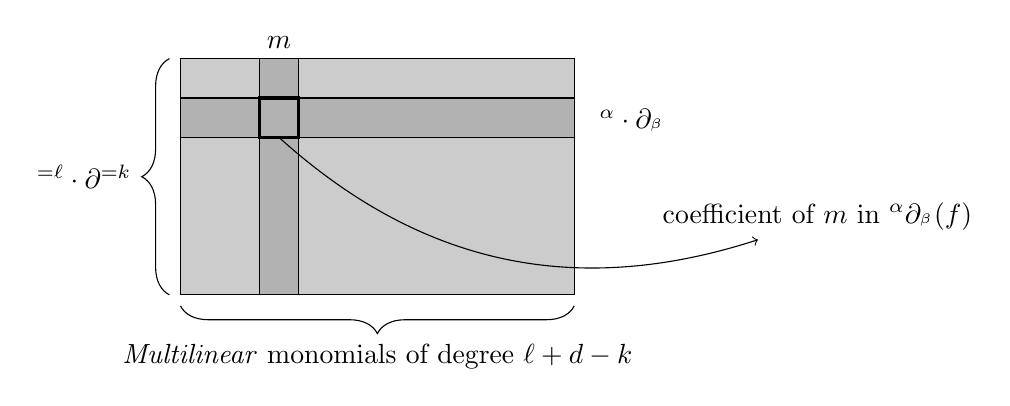
\begin{tikzpicture}
\draw[fill=black!20] (0,0) rectangle (5,3);

\draw[decorate,decoration={brace,amplitude=10pt,raise=4pt},yshift=0pt]
(0,0) -- (0,3);
\node[anchor=east] at (-0.5,1.5) {$\vecx^{=\ell} \cdot \partial^{=k}$};
\draw[decorate,decoration={brace,amplitude=10pt,mirror, raise=4pt},yshift=0pt] 
(0,0) -- (5,0);
\node[anchor=north] at (2.5,-0.5) {\emph{Multilinear} monomials of degree $\ell + d - k$};

\draw[fill=black!30] (1,0) rectangle (1.5,3);
\node at (1.25,3.2) {$m$};

\draw[fill=black!30] (0,2) rectangle (5,2.5);
\node[anchor=west] at (5.2,2.2) {$\vecx^{\alpha} \cdot \partial_{\vecx^\beta}$};

\draw[very thick] (1,2) rectangle (1.5,2.5);

\node[anchor=west] at (6,1) {coefficient of $m$ in $\vecx^\alpha \partial_{\vecx^\beta}(f)$}
edge[<-,bend left] (1.25,2);
\end{tikzpicture}


The works of \cite{KLSS,KS14} use this measure to prove a lower bound for ``\emph{low-support} depth $4$ circuits''. 
As sketched earlier, the task of proving lower bounds for general homogeneous depth $4$ circuits can be reduced to the \emph{low-support} depth $4$ circuits via random restrictions. 

\section{Reducing to `low-support' depth $4$ circuits}\label{sec:red-to-low-support}

We have already seen a sketch of how this can be done via a random restriction but let us formalize this as a lemma. 

\begin{lemma}\label{lem:red-to-low-supp}
Let $P$ be an $n$-variate degree $d$ polynomial computed by a homogeneous depth $4$ circuit $C$ of size $s \leq n^{c\sqrt{d}}$, for some $c>0$. 
Let $\rho$ be a random restriction that sets each variable to zero independently with probability $1 - 1/n^{2c}$. 
Then with probability at least $(1 - 1/s)$, the polynomial $\rho(P)$ is computed by a homogeneous depth $4$ circuit $C'$ with bottom support at most $\sqrt{d}$ and size at most $s$. 
\end{lemma}
\begin{proof}
Let $\inbrace{m_1,\dots, m_r}$ be the set of all monomials computed at the lowest layer of the depth $4$ circuit $C$ that are divisible by more than $\sqrt{d}$ distinct variables. 
Since the size of $C$ is at most $s$, we also have that $r\leq s$. 
Then,
\begin{eqnarray*}
\forall i\in [r] \qquad \Pr[\rho(m_i) \neq 0] & \leq & \frac{1}{n^{2c\sqrt{d}}}\\
\implies \qquad \Pr[\exists i \;:\; \rho(m_i) \neq 0] & \leq & \frac{r}{n^{2c\sqrt{d}}} \leq \frac{1}{n^{c\sqrt{d}}} \leq \frac{1}{s}
\end{eqnarray*}
Thus, with probability at least $(1 - 1/s)$, all the large support monomials are killed and $C$ reduces to a homogeneous depth $4$ circuit of bottom support at most $\sqrt{d}$. 
\end{proof}

\subsection{Handling random restrictions}

The previous section outlined how in essence, it would suffice to try and find an explicit polynomial for which we can prove a good enough lower bound for bounded bottom-support depth $4$ circuits. 
Let us say that we have found an explicit polynomial $g$ that requires depth $4$ circuits of size at least $n^{\sqrt{d}/100}$. 
Are we done? Let us write things down formally to see exactly what we need. 

Say the polynomial we wish to show requires large homogeneous depth $4$ circuits is $f$. 
Let us assume on the contrary that $f$ can be computed by homogeneous depth $4$ circuits of size $s < n^{\sqrt{d}/10000}$. 
Then, by \autoref{lem:red-to-low-supp}, $\rho(f)$ can be computed by a homogeneous depth $4$ circuits of bottom support bounded by $\sqrt{d}/1000$ of size $s$. 
We want to be able to say that this is a contradiction. 
We might be able to say that if $\rho(f)$ has $g$ as \emph{a projection}, that is, but setting more variables to zero in $\rho(f)$ we obtain $g$. 

Both the results of \cite{KLSS} and \cite{KS14} proceed by showing that the polynomial $g$, for which they show a lower bound for bounded bottom support circuits, is robust enough to yield the lower bound even after random restriction. 
The calculations become trickier because the calculations of $\Gamma^{[\mathrm{PSD}]}_{k,\ell}(\rho(f))$. 
However, in this survey we shall use an easier approach to generically lift any $g$ to a different polynomial $f$ such that $\rho(f)$ has $g$ as a projection. 
This trick came up during discussions with Mrinal Kumar. 

\begin{lemma}\label{lem:lin-transform-trick}
Let $\rho$ be a random restriction that sets each variable to zero independently with probability $1 - p$. 
For any polynomial $f(y_1,\dots y_n)$, define $f \circ \mathrm{Lin}_p$ as
\[
f \circ \mathrm{Lin}_p \spaced{=} f\inparen{\sum_{i=1}^t y_{1i}, \cdots, \sum_{i=1}^t y_{nt}}\quad \text{where $t = \inparen{\frac{1}{p}} n \log n$}
\]
Then, $\rho(f \circ \mathrm{Lin}_p)$ has $f$ as a projection with probability $1 - 1/2^{n}$. 
\end{lemma}
\begin{proof} For any $i = 1, \dots, n$
\begin{eqnarray*}
\quad \Pr[\rho(y_{i1}) = \dots \rho(y_{it}) = 0 ] & = & \inparen{1 - p}^t\\ 
& = & \frac{1}{n\cdot 2^n}\\
\implies \Pr[\exists i\;:\;\rho(y_{i1}) = \dots \rho(y_{it}) = 0 ]  & \leq  & \frac{1}{2^n} 
\end{eqnarray*}
Hence, with probability at least $1 - 1/2^n$, for each $i$ there is some $j$ such that $\rho(y_{ij}) \neq 0$. 
Therefore, with probability at least $1 - 1/2^n$, the polynomial $f$ is a projection of $\rho(f \circ \mathrm{Lin}_p)$. \end{proof}

In all the applications, as in \autoref{lem:red-to-low-supp}, we would have $p = 1/n^{O(1)}$. 
Thus, we would only incur a polynomial blow-up in the number of variables from $f$ to $f\circ \mathrm{Lin}_p$. 
Hence, we can focus on proving a lower bound  a homogeneous depth $4$ circuit of bottom support at most $r$ (which would eventually be something like $\sqrt{d}/100$). 

\begin{lemma}[\cite{KLSS}]\label{lem:upper-bound-low-supp}
Let $P$ be an $n$-variate degree $d$ polynomial computed by a homogeneous depth $4$ circuit of size $s$ and bottom-support at most $r$. 
Then for any $k,\ell$ such that $\ell + rk \leq n/2$, 
\[
\Gamma^{\mathrm{PSD}}_{k,\ell}(P) \quad \leq \quad s \cdot \binom{\frac{2d}{r}+k}{k}\cdot \binom{n}{\ell+rk}. 
\]
\end{lemma}

The proof of this lemma is exactly along the description in of Intuition - (2): split the circuit into multiquadratic and non-multiquadratic part, and show that the non-multiquadratic part contributes no multilinear monomials. 
But to just put things in perspective, we shall be dealing with parameters $r = \sqrt{d}/100$, $k = \sqrt{d}$ and $\ell = \frac{n}{2}(1 - \epsilon)$ for $\epsilon = O\inparen{\frac{\log d}{\sqrt{d}}}$. 
The above bound, by \autoref{lem:binom-approx}, can be seen to reduce to
\[
\Gamma^{\mathrm{PSD}}_{k,\ell}(P) \quad \leq \quad s \cdot \binom{n}{\ell} \cdot (1+\epsilon)^{2rk} \cdot 2^{O(\sqrt{d})}
\]


\subsection*{Sanity checks}

Let us first check if this measure can at least in principle yield a lower bound for us. 
The best way to do this is to get some heuristic estimate of what we expect the measure to be for a random $n$-variate degree $d$ polynomial $R$. \\

{\bf Heuristic Estimate. } For a random $n$-variate degree $d$ polynomial $R$, we expect the $\Gamma^{\mathrm{PSD}}_{k,\ell}(R)$ to be as large as it can be, i.e.
\[
\Gamma^{\mathrm{PSD}}_{k,\ell}(R) \spaced{\approx} \min\inparen{\binom{n}{k}\cdot \binom{n}{\ell}, \binom{n}{\ell + d-k}}
\]

As a first step, one should first check that if we could indeed find a polynomial $P$ for which the bound is as large as stated above, do we get a useful lower bound from \autoref{lem:upper-bound-low-supp}? Turns out that if we were to choose our parameters carefully, we do indeed get the lower bound. 
Just to give a sense of how \emph{careful} we need to be, here is some of the parameters that are chosen in \cite{KLSS,KS14}. 

\begin{itemize}
\item The number of variables $n$ is at least the cube of the degree $d$. 
\item The model we shall be working with is bottom-support $r$ where $r = \sqrt{d}/1000$. 
\item The order of derivatives $k = \sqrt{d}$. 
\item The degree of the shift $\ell$ shall be chosen as $\ell = \frac{n}{2}\inparen{1 - \epsilon}$ where $\epsilon = \frac{\log d}{c\sqrt{d}}$ for a suitable constant $c$. 
\end{itemize}

The above choice of parameters might already seem pretty fragile but these are not the most delicate choices! 
While proving the lower bound on $\Gamma^{\mathrm{PSD}}_{k,\ell}$ for an explicit polynomial, the number of monomials etc. need to be tailored to perfection to make the proof work. 

\section{The surrogate rank approach of \cite{KLSS}}

The goal is now to find an explicit polynomial $P$ such that $\mathrm{PSD}_{k,\ell}(P)$ has large rank. 
One way to prove that a set of polynomials are linearly independent is to show that they have distinct leading monomials (as used \cite{gkks13} etc.) Another method is to show that these polynomials are \emph{almost orthogonal}. 
An example of this phenomenon can be seen in the following fact. 

\begin{fact}
Let $M$ be a square matrix such that the absolute value of the diagonal entry is larger than sum of the absolute values of the non-diagonal entries in that row or column, i.e. $\abs{M_{ii}} \geq \sum_{j\neq i} \abs{M_{ij}}$ for all $i$. 
Then the matrix $M$ is full rank. 
\end{fact}

Such matrices are also called \emph{diagonally dominant matrices}, and captures the notion of \emph{almost orthogonal} vectors alluded to earlier. 
For symmetric matrices $M$, the following bound of Alon~\cite{Alo09}.

\begin{lemma}[\cite{Alo09}]\label{lem:trace-bound} For any real symmetric matrix $M$, 
\[
\rank(M) \spaced{\geq} \frac{(\mathrm{Tr}(M))^2}{\mathrm{Tr}(M^2)}
\]
\end{lemma}

We'll see the proof of this shortly but it would shed some more intuition to see what the above lemma yields for a diagonally dominant matrix. 
Let $M$ be a matrix of the form
\[
M \spaced{=} \insquare{\begin{array}{cccc}
D &  d & \dots &  d\\
 d & D & \dots & d\\
\vdots & \vdots & \ddots & \vdots \\
d & d & \dots & D
\end{array}}_{r \times r}
\]
Then, $\mathrm{Tr}(M) = D\cdot r$, and $\mathrm{Tr}(M^2) = (D^2 + (r-1)d^2)r = O(D^2 r + r^2 d^2)$. 
If $D > (r-1)d^2$, then $\mathrm{Tr}(M^2) = O(D^2r)$. 
Thus, the above lemma gives that $\rank(M) = \Omega(r)$. 
\begin{proof}
By the spectral theorem, any real symmetric matrix has a basis of eigen vectors with eigenvalues $\lambda_1,\dots, \lambda_n$ where $n$ is the dimension of the matrix. 
If $\lambda_1,\dots, \lambda_r$ are the non-zero eigenvalues, then 
\begin{eqnarray*}
\mathrm{Tr}(M) &   =  & \sum_{i=1}^r \lambda_i\\
& \leq & \sqrt{r} \;\cdot \; \inparen{\sum_{i=1}^r \lambda_i^2} = \sqrt{r}\;\cdot \; \mathrm{Tr}(M^2)\\
\implies r & \geq & \frac{(\mathrm{Tr}(M))^2}{\mathrm{Tr}(M^2)}
\end{eqnarray*}
\end{proof}

The bound of \cite{KLSS} for an explicit polynomial $P$ proceeds by considering the matrix $B$ where each row is indexed by a pair of multilinear monomials $(m_1,m_2)$  of degree $k$ and $\ell$ respectively, and the row is just the coefficients of the monomials of $\mathrm{mult}(m_2 \partial_{m_1}(P))$ in a fixed order. 
Note that $B$ is not even a square matrix, and certainly not symmetric. 
However, the matrix $M = B B^T$ is a symmetric square matrix such that $\rank(M) \leq \rank(B)$. \\

Let us spend some time understand the entries of $M$. 
The $(i,j)$-th entry of $M$ is precisely the inner-product of row $i$ and row $j$ of $B$. 
If $P$ is a polynomial with just zero-one coefficients, then the $i$-th diagonal entry is precisely the number of non-zero entries in row $i$ of $B$. 
Thus,
\begin{eqnarray*}
\mathrm{Tr}(M) & = & \text{number of non-zero entries in $B$}\\
  & = & \text{(\# cols of $B$)} \cdot \mathop{\mathbb{E}}_i[\text{\# non-zero entries in $i$-th col of $B$}] 
\end{eqnarray*}
The calculation for $\mathrm{Tr}(M^2)$ requires a little more care. 
Let $M_i$ refer to the $i$-th row of $M$ and $B_i$ refer to the $i$-th row of $B$. 
Then,
\begin{eqnarray*}
\mathrm{Tr}(M^2) & = & \sum_{i} \inangle{M_i, M_i}\\
 & = & \sum_{i} \sum_j \inangle{B_i, B_j}^2 \spaced{=}\sum_{i} \sum_j \inparen{\sum_m B_{im} B_{jm}}^2\\
 & = & \sum_{i} \sum_j \sum_m B_{im}^2 B_{jm}^2  \spaced{+} \sum_i \sum_j \sum_{m\neq m'} B_{im}B_{im'}B_{jm}B_{jm'}\\
 & = & \sum_{m} \inparen{\sum_i \sum_j B_{im} B_{jm}}  \spaced{+} \sum_i \sum_j \sum_{m\neq m'} B_{im}B_{im'}B_{jm}B_{jm'}\\
 & = & \quad\quad\quad T_1 \quad\quad\quad\quad\quad\quad + \quad\quad\quad\quad\quad\quad T_2
\end{eqnarray*}
The first term $T_1$ is easy to calculate:
\begin{eqnarray*}
T_1 & = & \text{(\# cols of $B$)} \cdot \mathop{\mathbb{E}}_i[\inparen{\text{\# non-zero entries in $i$-th col of $B$}}^2] \\
 & \stackrel{\tiny \text{(hopefully)}}{\approx} & \text{(\# cols of $B$)} \cdot \mathop{\mathbb{E}}_i[\inparen{\text{\# non-zero entries in $i$-th col of $B$}}]^2
\end{eqnarray*}
The term $T_2$ roughly corresponds to the number of $2\times 2$ submatrices of $B$ that is $\insquare{\begin{array}{cc}1 & 1 \\ 1 & 1\end{array}}$. 
If we could somehow show that there are not too many such submatrices, then $\mathrm{Tr}(M^2)$ is essentially dominated by $T_1$. 
That would then yield that $\rank(M) \gtrapprox \text{(\# cols of $B$)}$. 

\subsection*{Obtaining a bound on $T_2$:}

\[
T_2 \spaced{=} \sum_i \sum_j \sum_{m\neq m'} B_{im}B_{im'}B_{jm}B_{jm'}
\]
Each term $B_{im}B_{im'}B_{jm}B_{jm'}$ that is non-zero corresponds to a $2\times 2$ submatrix of $B$ (indexed by rows $i,j$ and columns $m,m'$) that is $\insquare{\begin{array}{cc} 1 & 1\\ 1&1
  \end{array}}$. \\

The columns of $B$ are indexed by multilinear monomials of degree $\ell + d - k$, and the rows of $B$ are indexed by a derivative and a shift. 
Let row $i$ correspond to $\mathrm{mult}(\gamma_1 \cdot \partial_{\alpha_1}(P))$ and row $j$ to $\mathrm{mult}(\gamma_1 \cdot \partial_{\alpha_1}(P))$. 
Thus, if the $2\times 2$ minor indexed by rows $i,j$ and columns $m,m'$ equals $\insquare{\begin{array}{cc} 1 & 1\\ 1&1 \end{array}}$, then there exists $\beta_1, \beta_2,\beta_3,\beta_4 \in P$ such that
\begin{eqnarray*}
m \spaced{=} \frac{\beta_1}{\alpha_1}\cdot \gamma_1 & = & \frac{\beta_3}{\alpha_2} \cdot  \gamma_2\\
m' \spaced{=} \frac{\beta_2}{\alpha_1}\cdot \gamma_1 & = & \frac{\beta_4}{\alpha_2}\cdot \gamma_2\\
\implies \frac{\beta_1}{\beta_3} & = & \frac{\beta_2}{\beta_4}
\end{eqnarray*}
Following notation used in \cite{KLSS}, we shall call $\beta_1,\beta_2,\beta_3,\beta_4$ as the \emph{label} of the $2\times 2$ minor. 
Since $m\neq m'$, we also have that $\beta_1 \neq \beta_2$. 
What we'd like to say that the only way $\beta_1/\beta_3 = \beta_2/\beta_4$ is if $\beta_3 = \beta_1$ and $\beta_2 = \beta_4$. 
This need not be true in general of course, but this is where the choice of the polynomial comes in. 

\begin{claim}
If $P$ is the $\NW_{d,d^3, e}$ polynomial for $e = \frac{d}{3}$ then any $2\times 2$ minor of $B$ (with the order of derivatives $k = o(d)$) that is $\insquare{\begin{array}{cc} 1&1\\1&1\end{array}}$ has label $\beta_1,\beta_2,\beta_3,\beta_4$ where $\beta_1 = \beta_3$ and $\beta_2 = \beta_4$, or $\beta_1 = \beta_2$ and $\beta_3 = \beta_4$. 
\end{claim}
\begin{proof}
Assume that $\beta_1 \neq \beta_3$. 
Then by \autoref{lem:NW-low-intersection} we know that they differ in at least $2d/3$ places. 
But then, $\beta_1/\beta_3 = \beta_2/\beta_4$ forces that $\beta_1$ and $\beta_3$ must agree at least $2d/3$ places forcing $\beta_1 = \beta_2$. 
\end{proof}

Thus, for the $\NW$-polynomial the number of such boxes is quite small. 
Using this, albeit with a reasonable amount of sweat, one can estimate $T_2$ to show that $T_2 = O(T_1)$. 
Thus, \cite{KLSS} obtain the following bound. 

\begin{lemma}[\cite{KLSS}]
For the polynomial $\NW_{d,d^3,e}$, for $e = \frac{d}{3}$, and $k = \sqrt{d}$ and $\ell = \frac{n}{2}\inparen{1 - \frac{\log d}{\sqrt{d}}}$ we have the bound
\[
\Gamma^{\mathrm{PSD}}_{k,\ell}(\NW_{d,d^3,e}) \spaced{\geq} \frac{1}{\poly(n,d)} \cdot \min\inparen{\binom{n}{\ell + d - k}, \binom{d}{k}^2 \cdot d^k \cdot k! \cdot \binom{n}{\ell}}
\]
\end{lemma}
Note that the first term of the $\min$ in the RHS is the number of columns of $B$, as we had heuristically estimated. 
Simplifying the RHS using \autoref{lem:binom-approx}, we get
\[
\Gamma^{\mathrm{PSD}}_{k,\ell}(\NW_{d,d^3,e}) \spaced{\geq} \frac{1}{\poly(n,d)} \cdot \binom{n}{\ell}\cdot \exp\inparen{c\cdot \epsilon (d - k)}
\]
for some constant $c > 0$. 
Since $\epsilon = \frac{\log d}{\sqrt{d}}$, we get 
\[
\Gamma^{\mathrm{PSD}}_{k,\ell}(\NW_{d,d^3,e}) \spaced{\geq} \frac{1}{\poly(n,d)} \cdot \binom{n}{\ell}\cdot \exp\inparen{c\cdot \sqrt{d}\cdot \log d}
\]
With the above bound and \autoref{lem:upper-bound-low-supp}, we get the lower bound of \cite{KLSS}. 
\begin{theorem}[\cite{KLSS}]\label{thm:KLSS-lowsupp}
Any depth $4$ homogeneous circuit of bottom support $r = \sqrt{d}/1000$ computing the polynomial $\NW_{d,d^3,d/3}$ over a characteristic zero field must have top fan-in $s = d^{\Omega(\sqrt{d})}$. 

In fact, more generally, any homogeneous depth $4$ circuit of bottom support bounded by $r$ computing $\NW_{d,m,e}$ for suitably chosen parameters must have top fanin $s = d^{\Omega(d/r)}$. 
\end{theorem}

Coupling with \autoref{lem:lin-transform-trick}, we obtain (a slight reformulation of) their main theorem. 

\begin{theorem}[\cite{KLSS}]\label{thm:KLSS-main}
Any depth $4$ homogeneous computing the polynomial $\NW_{d,d^3,d/3}\circ \mathrm{Lin}$ over a characteristic zero field must have size $s = d^{\Omega(\sqrt{d})}$. 
\end{theorem}

\section{The leading monomial approach of \cite{KS14}}

Shortly after \cite{KLSS}, a purely combinatorial proof of the result was presented by Kumar and Saraf~\cite{KS14}. 
More over, they were able to prove the lower bound of $n^{\Omega(\sqrt{d})}$ for the size of any homogeneous depth $4$ circuit computing $\IMM_{n,d}$ (for some suitable choices of $n$ and $d$). 
This was a strengthening of \cite{KLSS} in two ways -- (1) it worked over any field, and (2) the lower bound was for a polynomial that we know can be computed small arithmetic circuit. 

The calculations of \cite{KS14} are much more trickier than \cite{KLSS} but there are quite a few interesting ideas that would even have application in other areas. \\

The earlier lower bounds of \cite{gkks13,KSS13,FLMS13} required a lower bound on the dimension of shifted partial derivatives of a polynomial $P$, and this was obtained by finding a \emph{large} set of \emph{distinct leading monomials}. 
In \cite{KS14}, they take this approach but require a very careful analysis. 
The key difference in this setting is the following: 

\begin{quote}
  If $\beta$ is the leading monomial of a polynomial $P$, then for any monomial $\gamma$, we also have that $\beta \cdot \gamma$ is the leading monomial of $\gamma P$. 

  However, the leading monomial of $\mathrm{mult}(\gamma P)$ could be $\beta' \cdot \gamma$ for some $\beta' \neq \beta$ (as higher monomials could be made non-multilinear during the shift by $\gamma$). 
\end{quote}

The multilinear projection makes the task of counting leading monomials much harder and \cite{KS14} come up with a clever method to estimate this. 

\subsection*{Leading monomials after multilinear projections}

Let $P$ the polynomial for which we are trying to lower bound $\Gamma^{\mathrm{PSD}}_{k,\ell}(P)$. 
For every monomial multilinear monomial $\alpha$ of degree $k$, and a monomial $\beta \in \partial_\alpha(P)$, define the set $A(\alpha, \beta)$ as
\[
A(\alpha, \beta) \spaced{=} \setdef{\gamma}{\begin{array}{c}\deg(\gamma) = \ell + d - k\;\text{and there is a $\gamma'$ of degree $\ell$}\\\text{such that }\gamma  = \mathrm{LM}(\mathrm{mult}(\gamma' \cdot \partial_\alpha(P))) = \gamma' \cdot \beta \end{array}}
\]
In other words, we want the number of distinct monomials that are contributed by $\beta$, which are also distinct leading monomials obtained from $\partial_\alpha(P)$ that are divisible by $\beta$. 
We then have
\begin{equation}\label{eqn:union-of-As}
\Gamma^{\mathrm{PSD}}_{k,\ell}(P) \spaced{\geq} \abs{\Union_{\alpha, \beta} A(\alpha, \beta)}
\end{equation}

\noindent
{\bf Choice of derivatives:} Instead of looking at all derivatives in  $\partial^{=k}$, we shall restrict ourselves to just a subset of derivatives. Restricting the above union to a subset $\Delta  \subset \vecx^{=k}$ still continues to remain a lower bound for $\Gamma^{\mathrm{PSD}}_{k,\ell}(P)$. Keeping in mind that we are dealing with $P = \NW_{d,m,e}$ we shall choose $\Delta$ to be a set of monomials of the form $x_{1a_1}\cdots x_{ka_k}$ with each $a_i \leq m$ so as to have $m^k$ derivatives in total. This shall become relevant later. 
\begin{equation}\label{eqn:union-of-As}
\Gamma^{\mathrm{PSD}}_{k,\ell}(P) \spaced{\geq} \abs{\Union_{\substack{\alpha \in \Delta \\\beta \in \vecx^{=\ell}}} A(\alpha, \beta)}
\end{equation}

The standard technique to obtain a lower bound on the union of sets is via the \emph{Inclusion-Exclusion} principle. 

\begin{lemma}[Inclusion-Exclusion Principle]\label{lem:inc-exc}
For any collection of sets $A_1,\dots, A_r$,
\[
\abs{\Union_i A_i} \spaced{\geq} \sum_{i} \abs{A_i} \spaced{-} \sum_{i\neq j}\abs{A_i\intersection A_j}
\]
\end{lemma}

If we were to somehow show that $\sum_{i\neq j}\abs{A_i\intersection A_j} \leq \frac{1}{2}\sum_i \abs{A_i}$, then we obtain that $\abs{\union_i A_i} \geq \frac{1}{2}\cdot \sum_i \abs{A_i}$. 
This is what shall be employed for the sets $A(\alpha, \beta)$, except that we quickly run into two immediate problems. 

\begin{enumerate}
  \item How do we even estimate $A(\alpha, \beta)$? The set of $\gamma'$ such that $\gamma' \beta = \mathrm{LM}(\partial_\alpha(P))$ do not seem to have any nice combinatorial structure. 
  \item What if it so happens that $\sum \abs{A(\alpha_1,\beta_1)\intersection A(\alpha_2,\beta_2)} = 100 \sum \abs{A(\alpha,\beta)}$? Inclusion-Exclusion does not yield anything in that case. 
\end{enumerate}


It so turns out that the second point actually is the case. 
In fact for $\IMM_{n,d}$, the second term turns out to be greater than the first term by a factor of $n^{\sqrt{d}/1000}$ or so! 
In \cite{KS14}, they prove a wonderful strengthened version of the Inclusion-Exclusion principle which allows them to handle the second hurdle. 

\begin{lemma}[Stronger Inclusion-Exclusion \cite{KS14}]\label{lem:str-inc-exc}
Let $A_1,\dots, A_r$ be sets such that there is some $\lambda > 1$ such that
\[
\sum_{i\neq j} \abs{A_i \intersection A_j} \spaced{\leq} \sum_i \lambda \cdot \abs{A_i}
\]
Then, 
\[
\abs{\Union_i A_i} \spaced{\geq} \inparen{\frac{1}{4\lambda}} \cdot \inparen{\sum_i \abs{A_i}}
\]
\end{lemma}

In other words, as long as the second term of the Inclusion-Exclusion principle is \emph{not too much larger} than the first term, we still can get non-trivial bounds on the union. 

\begin{proof}
Let $p = \frac{1}{2\lambda} < 1$. 
Define sets $A_1',\dots, A_r'$ such that $A_i' \subseteq A_i$ obtained by adding each element of $A_i$ to $A_i'$ independently with probability $p$. 
Since $A_i' \subseteq A_i$, we also have that $\abs{\union A_i} \geq \abs{\union  A_i'}$. 
By linearity of expectation, 
\[
\E\insquare{\sum_i \abs{A_i'}} \spaced{=} p \sum_{i} \abs{A_i} 
\]
More importantly, by the sampling process,
\[
\E\insquare{\abs{A_i' \intersection A_j'}} \spaced{=} p^2 \cdot \abs{A_i \intersection A_j}
\]
as any common element must be added to both $A_i'$ \emph{and} $A_j'$, and either of these events happen independently with probability $p$ each. 
Since $\sum_{i,j}\abs{A_i' \intersection A_j'}$ drops by a factor of $p^2$, we are now in a position to apply the \autoref{lem:inc-exc} to the $A_i'$s. 
\begin{eqnarray*}
\abs{\Union A_i} & \geq &  \E\insquare{\abs{\Union A_i'}}\\
& \geq & \E\insquare{\sum_i \abs{A_i'}} \spaced{-} \E\insquare{\abs{A_i' \intersection A_j'}}\\
& = & p \inparen{\sum_i \abs{A_i}} \spaced{-} p^2\inparen{\sum_{i\neq j}\abs{A_i \intersection A_j}}\\
& \geq & p \inparen{\sum_i \abs{A_i}} \spaced{-} p^2 \lambda \inparen{\sum_i \abs{A_i}}\\
& \geq & \frac{p}{2} \inparen{\sum_i \abs{A_i}} \spaced{=} \frac{1}{4\lambda} \inparen{\sum_i \abs{A_i}}
\end{eqnarray*}
\end{proof}

\begin{corollary}\label{cor:inc-exc-str}
Considers sets $A_1,\dots, A_r$  and let $S_1 = \sum_i \abs{A_i}$ and $S_2 = \sum_{i\neq j} \abs{A_i \intersection A_j}$. 
Then, 
\[
\abs{\Union A_i} \spaced{\geq} \frac{S_1}{4} \cdot \min\inparen{1,\frac{S_1}{S_2}}
\]
\end{corollary}

We can now proceed to lower bound $\abs{\Union A(\alpha, \beta)}$ via inclusion exclusion.

\subsection*{Estimating $\abs{\Union A(\alpha, \beta)}$ via Inclusion-Exclusion}
\[
\abs{\Union_{\alpha, \beta}A(\alpha,\beta)}\spaced{\geq} \sum_{\alpha,\beta}\abs{A(\alpha, \beta)} \spaced{-} \sum_{(\alpha, \beta)\neq (\alpha',\beta')}\abs{A(\alpha, \beta) \intersection A(\alpha',\beta')}
\]

Let us first address the term $\sum \abs{A(\alpha, \beta)}$. 
As mentioned earlier, it is not an easy task to get a good handle on the set $A(\alpha, \beta)$ for polynomial such as $\NW$ or $\IMM$, for any reasonable monomial ordering. 
However, \cite{KS14} circumvent this difficult by using an indirect approach to estimate this term. 

For any derivative $\alpha$ and $\beta \in \partial_\alpha(P)$, define the set $S(\alpha, \beta)$ as the following set of multilinear monomials of degree $\ell$ that is disjoint from $\beta$. 
\[
S(\alpha, \beta) \spaced{=} \setdef{\gamma}{\begin{array}{c}\text{$\gamma$ is multilinear, has}\\\text{degree $\ell$ and $\gcd(\beta,\gamma)=1$ }\end{array}}
\]
This on the other hand is independent of any monomial ordering, and is also easy to calculate:
\[
\text{For every $\alpha, \beta$}\quad\quad \abs{S(\alpha, \beta)} \spaced{=} \binom{n - d + k}{\ell}.
\] 
\begin{lemma}[\cite{KS14}]\label{lem:As-to-Ss}
For any $\alpha$, 
\[
\sum_{\beta} \abs{A(\alpha, \beta)} \spaced{\geq} \abs{\Union_{\beta} S(\alpha, \beta)}
\]
\end{lemma}
\begin{proof}
Consider any $\gamma \in \Union_{\beta}S(\alpha, \beta)$. 
By definition, there is at least one non-multilinear monomial in $\gamma \cdot \partial_\alpha(P)$. 
Thus, in particular $\mathrm{LM}(\mathrm{mult}(\gamma \cdot \partial_\alpha(P))$ is non-zero and equal to some $\gamma \cdot \beta$ for some monomial $\beta \in \partial_\alpha(P)$. 
This also implies that $\gamma' = \gamma\cdot \beta \in A(\alpha, \beta)$. 
This yields an injective map $\phi$ 
\[
\phi:\Union_\beta S(\alpha,\beta) \spaced{\rightarrowtail} \setdef{(\beta, \gamma')}{\beta\in \partial_\alpha(P)\;,\;\gamma' \in A(\alpha, \beta)}
\] 
Since the size of the RHS is precisely $\sum_\beta \abs{A(\alpha, \beta)}$, the lemma follows. 
\end{proof}

Thus, by another use of Inclusion-Exclusion on the $S(\alpha, \beta)$'s, we get
\begin{eqnarray*}
\abs{\Union_{\alpha, \beta}A(\alpha,\beta)}&\geq& \sum_{\alpha,\beta}\abs{A(\alpha, \beta)} \spaced{-} \sum_{(\alpha, \beta)\neq (\alpha',\beta')}\abs{A(\alpha, \beta) \intersection A(\alpha',\beta')}\\
 & \geq & \sum_\alpha \inparen{\sum_\beta \abs{S(\alpha, \beta)}} \spaced{-} \sum_\alpha \inparen{\sum_{\beta \neq \beta'}\abs{S(\alpha, \beta)\intersection S(\alpha,\beta')}}\\
 & & \quad\quad \spaced{-} \sum_{(\alpha, \beta)\neq (\alpha',\beta')}\abs{A(\alpha, \beta) \intersection A(\alpha',\beta')}
\end{eqnarray*}
Let us call the three terms in the RHS of the last equation as $T_1$, $T_2$ and $T_3$ respectively. 
Since we know the size of each $S(\alpha, \beta)$ exactly, the value of $T_1$ is easily obtained. 
\begin{lemma}[\cite{KS14}]\label{lem:T_1-value}
\begin{eqnarray*}
T_1(\alpha) \spaced{:=} \sum_{\beta}\abs{S(\alpha,\beta)}&=&\text{(\# mons in a deriv)} \cdot \binom{n-d+k}{\ell}
\end{eqnarray*}
\end{lemma}

\noindent
We shall be simplifying such binomial coefficients very often so let us recall the \autoref{lem:binom-approx}. 

\binomapprox*

\noindent
Since our of parameters would be $\epsilon = \Theta\inparen{\frac{\log d}{\sqrt{d}}}$, the bound on $T_1$ can be simplified as
\begin{eqnarray*}
T_1(\alpha)  & =  &\text{(\# mons in a deriv)} \cdot \binom{n}{\ell} \cdot \inparen{\frac{1+\epsilon}{2}}^{d-k} \cdot \exp(O(\log^2 d))\\
& = & m^{e-k}\cdot \binom{n}{\ell} \cdot \inparen{\frac{1+\epsilon}{2}}^{d-k} \cdot \exp(O(\log^2 d))
\end{eqnarray*}
\begin{remark*}To avoid writing this factor of $\exp(O(\log^2 d))$, we shall use $\approx$ of $\gtrsim$ or $\lesssim$ to indicate that a factor $\exp(O(\log^2 d))$ is omitted. 
\end{remark*}

\bigskip

So far we have not used any property of the polynomial $P$. 
But this becomes crucial in the calculation of $T_2$ and $T_3$. 
To get a sense of how these calculations proceed in \cite{KS14}, we present the full calculation for the case of $P = \NW_{d,m,e}$ for suitable choices of the parameters $m,d,e$. 
\begin{lemma}[\cite{KS14}]\label{lem:T_2-for-NW}
For the polynomial $\NW_{d,m,e}$, if $n = md$ and $\ell = \frac{n}{2}(1 - \epsilon)$ for $\epsilon = \Theta\inparen{\frac{\log d}{\sqrt{d}}}$, for every $\alpha \in \Delta$, 
\[
T_2(\alpha)\spaced{:=} \sum_{\beta\neq \beta'}\abs{S(\alpha, \beta)\intersection S(\alpha, \beta')} \quad \lesssim \quad m^{2(e-k)}\cdot \binom{n}{\ell} \cdot \inparen{\frac{1+\epsilon}{2}}^{2d -2k} 
\]
\end{lemma}
\begin{proof}
Recall that $S(\alpha,\beta) \intersection S(\alpha,\beta')$ is just set of all multilinear monomials $\gamma$ of degree $\ell$ that are disjoint from both $\beta$ and $\beta'$.
Hence, for any pair of multilinear degree $(d-k)$ monomials $\beta \neq \beta' \in \partial_\alpha(P)$ such that $\deg(\gcd(\beta, \beta')) = t$, we know that 
\[
\abs{S(\alpha, \beta)\intersection S(\alpha, \beta')} \spaced{=} \binom{n - 2d + 2k +t}{\ell}
\]
Thus, if we can count the number of pairs $(\beta, \beta')$ that agree on exactly $t$ places, we can obtain $T_2(\alpha)$. 
Note that for $\NW_{d,m,e}$, any two $\beta, \beta' \in\partial_\alpha(\NW_{d,m,e})$ can agree on at most $e-k$ places. 
Further, the number of pairs that agree in exactly $0\leq t\leq e-k$ places is at most
\[
m^{e-k} \cdot \binom{d-k}{t} \cdot (m-1)^{e-k-t}
\]
as there are $m^{e-k}$ choices for $\beta$, and $\binom{d-k}{t}$ choices for places where they may agree, and $(m-1)^{e-k-t}$ choices for $\beta'$ that agree with $\beta$ on those $t$ places. 
Thus,
\begin{eqnarray*}
T_2(\alpha) &\leq& \sum_{t=0}^{e-k} m^{e-k} \cdot \binom{d-k}{t} \cdot (m-1)^{e-k-t} \cdot  \binom{n - 2d + 2k +t}{\ell}\\
& \approx  & \sum_{t=0}^{e-k} m^{e-k} \cdot \binom{d-k}{t} \cdot (m-1)^{e-k-t} \cdot  \binom{n}{\ell} \frac{1}{2^{2d-2k -t}}\cdot (1+\epsilon)^{2d - 2k - t}\\
& \leq & m^{2(e-k)}\binom{n}{\ell}\inparen{\frac{1+\epsilon}{2}}^{2d -2k}\cdot\sum_{t=0}^{e-k}\binom{d-k}{t}\inparen{\frac{2}{(1+\epsilon)m}}^t\\
& \leq & m^{2(e-k)}\binom{n}{\ell}\inparen{\frac{1+\epsilon}{2}}^{2d -2k}\cdot \inparen{1+\frac{2}{(1+\epsilon)m}}^{d-k}\\
& = & m^{2(e-k)}\cdot \binom{n}{\ell} \cdot \inparen{\frac{1+\epsilon}{2}}^{2d -2k}\cdot O(1) \qquad\text{if $m = \Omega(d)$}\qedhere
\end{eqnarray*}
\end{proof}
\noindent
Combining this with \autoref{lem:T_1-value} and using Inclusion-Exclusion (\autoref{cor:inc-exc-str}),
\begin{eqnarray*}
\abs{\Union_{\beta} S(\alpha,\beta)} &\spaced{\gtrsim}& T_1(\alpha) \cdot \min\inparen{1,\frac{T_1(\alpha)}{T_2(\alpha)}}\\
& \approx & T_1(\alpha) \cdot \min\inparen{1,\frac{\pfrac{2}{1+\epsilon}^{d-k}}{m^{e-k}}}
\end{eqnarray*}
To maximize this, if we choose the parameters $m,d,e$ such that $T_1(\alpha) \approx T_2(\alpha)$, we obtain the following corollary. 
\begin{corollary}\label{cor:T2-bound}
Consider the polynomial $\NW_{d,m,e}$ with $n = md$ and $m = \Omega(d)$. 
If $\ell = \frac{n}{2}(1 - \epsilon)$ for $\epsilon = \Theta\inparen{\frac{\log d}{\sqrt{d}}}$ and $e$ chosen so that
\[
m^{e-k} \quad \stackrel{\poly}{=} \quad \inparen{\frac{2}{1+\epsilon}}^{d-k}
\]
then
\[
\sum_{\substack{\alpha \in \Delta\\\beta \in \partial_\alpha(\mathrm{NW})}}\abs{A(\alpha, \beta)} \spaced{\gtrsim} \abs{\Delta}\cdot  \binom{n}{\ell}
\]
\end{corollary}
\begin{proof}
By \autoref{lem:As-to-Ss}, we know that
\[
\sum_{\substack{\alpha\in \Delta\\\beta \in \partial_\alpha(P)}} \abs{A(\alpha,\beta)} \spaced{\geq} \abs{\Delta} \cdot \abs{\Union_{\beta} S(\alpha,\beta)}.
\]
Furthermore, from the discussion above, if $T_1(\alpha) \approx T_2(\alpha)$ then
\begin{eqnarray*}
\abs{\Union_{\beta}S(\alpha, \beta)} &\gtrsim &  T_1(\alpha) \cdot \min\inparen{1,\frac{T_1(\alpha)}{T_2(\alpha)}}\\
 & = & T_1(\alpha)\\
 & \approx & \binom{n}{\ell}
\end{eqnarray*}
as $T_1(\alpha) \approx T_2(\alpha)$ forces $m^{e-k} \approx \inparen{\frac{2}{1+\epsilon}}^{d-k}$. Therefore,
\[
\sum_{\substack{\alpha\in \Delta\\\beta \in \partial_\alpha(P)}} \abs{A(\alpha,\beta)} \spaced{\gtrsim} \abs{\Delta} \cdot \binom{n}{\ell}\qedhere
\]
\end{proof}

Note that $e$ needs to tailored very precisely to force the above condition! 
If $e$ is chosen too large or small, we get nothing from this whole exercise!

In the case of $\IMM$ this calculations gets a lot messier. 
The calculation would similarly force that the number of monomials must be in a very narrow range. 
This is achieved by instead looking at a random subgraph of the generic ABP of suitable sparsity to ensure the following two properties:
\begin{itemize}
  \item The number of monomials in any derivative is exactly as demanded. 
  \item `Most' pairs of monomials $(\beta, \beta')$ agree on `few' places. 
\end{itemize}

\subsection*{Upper bounding $\sum \abs{A(\alpha,\beta)\intersection A(\alpha',\beta')}$}

We are still left with the task of upper bounding
\[
T_3 \quad = \quad \sum_{(\alpha, \beta)\neq (\alpha',\beta')} \abs{A(\alpha, \beta) \intersection A(\alpha',\beta')}
\]
As mentioned earlier, we really do not have a good handle on the set $A(\alpha, \beta)$, and certainly not on the intersection of two such sets. 
Once again, we shall use a proxy that is easier to estimate to upper bound $T_3$. 

The set $A(\alpha, \beta) \intersection A(\alpha',\beta')$ consists of multilinear monomials $\gamma$ of degree $\ell + d -k$ such that there exists multilinear monomials $\gamma', \gamma''$ of degree $\ell$ satisfying
\begin{eqnarray*}
\gamma & = & \gamma' \beta \spaced{=} \gamma'' \beta',\\
 \gamma'\beta & = & \mathrm{LM}(\mathrm{mult}(\gamma' \partial_\alpha(P)))\\
\text{and}\quad \gamma''\beta' & = & \mathrm{LM}(\mathrm{mult}(\gamma'' \partial_{\alpha'}(P)))
\end{eqnarray*}
This in particular implies that $\gamma$ must be divisible by both $\beta$ and $\beta'$. 

\begin{observation}\label{obs:T3-proxy}
If $\deg(\gcd(\beta, \beta')) = t$, then
\[
\abs{A(\alpha, \beta) \intersection A(\alpha', \beta')} \spaced{\leq} \binom{n - 2d + 2k + t}{\ell - d + k +t}
\]
\end{observation}
\begin{proof}
Every monomial $\gamma \in A(\alpha, \beta) \intersection A(\alpha', \beta')$ must be divisible by $\beta$ and $\beta'$. 
Since $\abs{\beta \union \beta'} = 2d - 2k - t$, the number of choices of $\gamma$ is precisely
\[
\binom{n - (2d - 2k -t)}{(\ell + d - k) - (2d - 2k - t)} \quad = \quad \binom{n - 2d + 2k + t}{\ell - d + k + t}\qedhere
\]
\end{proof}

One needs a similar argument as in the case of $T_2$ to figure out how many pairs $(\alpha, \beta) \neq (\alpha',\beta')$ are there with $\deg(\gcd(\beta, \beta')) = t$ and sum them up accordingly. 

\begin{lemma}[\cite{KS14}] \label{lem:T3-bound}
For the polynomial $\NW_{d,m,e}$, and $n = md$ and $\ell = \frac{n}{2}(1 - \epsilon)$ for $\epsilon = \Theta\inparen{\frac{\log d}{\sqrt{d}}}$, 
\[
T_3 \quad \lesssim \quad \abs{\Delta}^2 \cdot \pfrac{m^{e-k}}{2^{d-k}}^2 \cdot \binom{n}{\ell}
\]
\end{lemma}
\begin{proof}
Fix a pair of derivatives $\alpha,\alpha'$. 
As before, we shall first count the number of pairs of monomials $\beta \in \partial_\alpha P$ and $\beta' \in \partial_{\alpha'} P$ such that $\gcd(\beta, \beta') = t$. 
Note that since $\alpha$ may differ from $\alpha'$, we could potentially have $\gcd(\beta_1,\beta_2) = e$. 
Once again, this is easily seen to be at most
\[
m^{e-k} \cdot \binom{d-k}{t} \cdot (m-1)^{e-k-t}. 
\]
\noindent Therefore, using \autoref{obs:T3-proxy}, 
\begin{eqnarray*}
T_3(\alpha, \alpha') & \leq & \sum_{t=0}^{e} m^{e-k} \cdot (m-1)^{e-k -t} \binom{d-k}{t} \binom{n- 2d + 2k +t}{\ell - d + k + t}\\
& \approx & \sum_{t=0}^{e} m^{e-k} \cdot (m-1)^{e-k -t} \binom{d-k}{t} \cdot \binom{n}{\ell} \inparen{\frac{1}{2}}^{2d - 2k -t}  (1+\epsilon)^{t}\\
& \leq & \frac{m^{2(e-k)}}{2^{2(d-k)}} \cdot \binom{n}{\ell} \cdot \inparen{1 + \frac{2(1+\epsilon)}{m}}^{d-k}\\
& \approx & \frac{m^{2(e-k)}}{2^{2(d-k)}} \cdot \binom{n}{\ell} \qquad\text{(as $m = \Omega(d)$)}\\
\implies T_3 & \lesssim & \abs{\Delta}^2 \cdot \pfrac{m^{e-k}}{2^{d-k}}^2 \cdot \binom{n}{\ell}
\qedhere
\end{eqnarray*}
\end{proof}
\noindent
Recalling that we have chosen our parameters so that 
\[
\text{(\# mons per deriv)} \approx \inparen{\frac{2}{1+\epsilon}}^{d-k}
\]
the above equation reduces to 
\[
T_3 \quad \lesssim \quad \abs{\Delta}^2 \inparen{\frac{1}{1+\epsilon}}^{2(d-k)} \cdot \binom{n}{\ell}.
\]
We shall choose our set of derivatives so that $\abs{\Delta} \approx (1+\epsilon)^{2(d-k)}$. 
With that setting, we can readily see that $T_3 \lesssim T_1$. 

Combining with \autoref{cor:T2-bound}, we obtain the required bound for $\abs{\Union A(\alpha, \beta)}$ via Inclusion-Exclusion (\autoref{cor:inc-exc-str}). 

\begin{lemma}\label{lem:d4hom-goldilocks-LB}
Let $m = d^2$ (so that $n = md = d^3$). 
Let $k = O(\sqrt{d})$ and  $\ell  = \frac{n}{2}\inparen{1 - \epsilon}$ for $\epsilon = \frac{\log d}{c \sqrt{d}}$ where $c$ is a constant. 
If $c$ and $e$ are tailored so that 
\begin{eqnarray*}
 \abs{\Delta} \spaced{=} m^k & \gtrsim &  (1+\epsilon)^{2d - 2k}\\
 m^{e-k} & \approx & \inparen{\frac{2}{1+\epsilon}}^{d-k}
\end{eqnarray*}
Then, for the polynomial $\NW_{d,m,e}$, if we consider a subset of non-zero derivatives order $k$ of size $\floor{(1+\epsilon)^{2d - 2k}}$, then
\[
\Gamma^{\mathrm{PSD}}_{k,\ell}(\NW_{d,m,e})\spaced{\geq}\abs{\Union_{\alpha, \beta} A(\alpha, \beta)} \spaced{\gtrsim} \binom{n}{\ell} \cdot (1+\epsilon)^{2d-2k}.
\] 
\end{lemma}

By \autoref{lem:upper-bound-low-supp}, we know that any homogeneous depth-$4$ circuit $C$ of size $s$ and bottom fan-in $r$ satisfies
\[
\Gamma^{\mathrm{PSD}}_{k,\ell}(C)\spaced{\leq} s \cdot \binom{n}{\ell} \cdot (1+\epsilon)^{rk} \cdot 2^{O(\sqrt{d})}.
\]
Hence, if $r$ was small enough (say $r = \sqrt{d}/1000$) so that $rk \leq (d-k)$, then we have a lower bound of $s \geq (1+\epsilon)^{d-k} \cdot 2^{O(\sqrt{d})}$ which is $d^{\Omega(\sqrt{d})}$ by the choice of $\epsilon$. 
\begin{theorem}[\cite{KS14}]\label{thm:IMM-lowsup-lb}
Any homogeneous depth $4$ circuit with bottom support bounded by $r = \sqrt{d}/1000$ computing, over any field $\F$, the polynomial $\NW_{d,m,e}$ with parameters as defined above must have top fan-in $s = d^{\Omega(\sqrt{d})}$. 

In fact, more generally, any homogeneous depth $4$ circuit of bottom support bounded by $r$ computing $\NW_{d,m,e}$ for suitably chosen parameters must have top fanin $s = d^{\Omega(d/r)}$. 
\end{theorem}

Again, coupling with \autoref{lem:lin-transform-trick}, we obtain (a slight reformulation of) their theorem. 

\begin{theorem}[\cite{KLSS,KS14}]\label{thm:IMM-lb}
Any homogeneous depth $4$ circuit computing, over any field $\F$,  the polynomial $\NW_{d,m,e}\circ \mathrm{Lin}$ with parameters as defined above must have top fan-in $s = d^{\Omega(\sqrt{d})}$. 

A similar lower bound $d^{\Omega(\sqrt{d})}$ holds also for the polynomial $\mathrm{IMM}_{n,d} \circ \mathrm{Lin}$ for suitable choices of $n$ and $d$. 
\end{theorem}

\begin{exercise} Show that the there indeed does exist settings of $c$ and $e$ so as to satisfy the constraints in \autoref{lem:d4hom-goldilocks-LB}.
\end{exercise}


%%% Local Variables: 
%%% mode: latex
%%% TeX-master: "main"
%%% End: 


\part{Further applications of shifted partial derivatives}

\chapter{Quick summary of key points}

The chapters that follow would delve deeper to show more general models where variants of shifted or projected shifted partial derivatives can be used to prove lower bounds.
A lot of the lower bounds would use specific observation or tricks used in the proofs in \autoref{chap:d4-bottomfanin} and \autoref{chap:d4hom}. 

\mdfsetup{%
roundcorner=5pt
}
\begin{quote}
\begin{mdframed}
{\bf Note to reader:} All these lower bounds would involve a delicate play between the various parameters involved. In order to completely understand, it is \emph{imperative} that you work out the calculations in \autoref{chap:d4-bottomfanin} and \autoref{chap:d4hom} (specifically those in \autoref{sec:KS-leading-monomial-approach}) at least once completely. Doing that would give some sense of how the different parameters interact and this is crucial to a lot of the lower bounds that follow. 
\end{mdframed}
\end{quote}

Having said that, this chapter shall be devoted to restating the most important points to remember from the previous two chapters.
These would be enough to get a high-level view of the lower bounds that follow but one has to get their hands dirty somewhere to completely understand these.

\section{Shifted Partial Derivatives}

\begin{definition*}[Shifted Partial Derivatives, \autoref{defn:shifted-partials}]
  Let $\partial^{=k}(f)$ refer to the set of all $k$-th order partial derivatives of $f$, and $\vecx^{\leq \ell}$ refer to the set of all monomials of degree at most $\ell$. 
The \emph{shifted partials of $f$}, denoted by $\SPD{k}{\ell}{f}$, is the vector space spanned by $\inbrace{\vecx^{\leq \ell} \cdot \partial^{=k}(f)}$. 
The dimension of this space shall be denoted by $\CM{SPD}_{k,\ell}(f)$. 
\end{definition*}

\noindent
To express this pictorially, $\CM{SPD}_{k,\ell}(f)$ is the rank of the following matrix. 

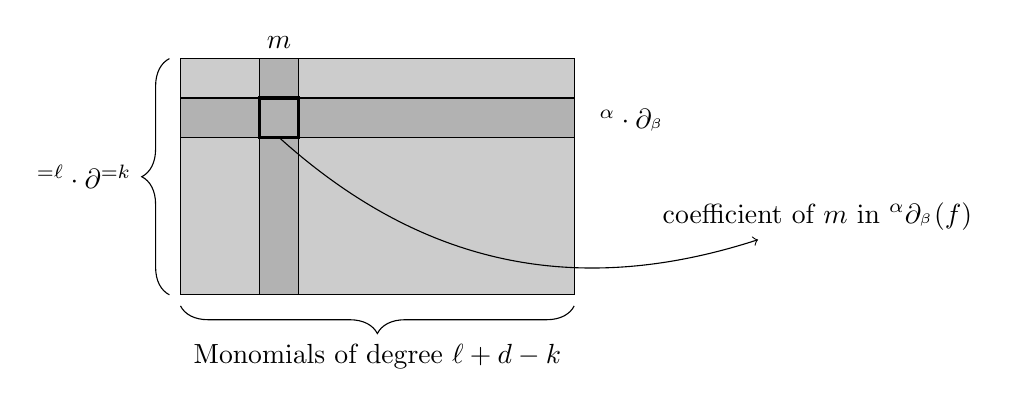
\begin{tikzpicture}
\draw[fill=black!20] (0,0) rectangle (5,3);

\draw[decorate,decoration={brace,amplitude=10pt,raise=4pt},yshift=0pt]
(0,0) -- (0,3);
\node[anchor=east] at (-0.5,1.5) {$\vecx^{=\ell} \cdot \partial^{=k}$};
\draw[decorate,decoration={brace,amplitude=10pt,mirror, raise=4pt},yshift=0pt] 
(0,0) -- (5,0);
\node[anchor=north] at (2.5,-0.5) {Monomials of degree $\ell + d - k$};

\draw[fill=black!30] (1,0) rectangle (1.5,3);
\node at (1.25,3.2) {$m$};

\draw[fill=black!30] (0,2) rectangle (5,2.5);
\node[anchor=west] at (5.2,2.2) {$\vecx^{\alpha} \cdot \partial_{\vecx^\beta}$};

\draw[very thick] (1,2) rectangle (1.5,2.5);

\node[anchor=west] at (6,1) {coefficient of $m$ in $\vecx^\alpha \partial_{\vecx^\beta}(f)$}
edge[<-,bend left] (1.25,2);
\end{tikzpicture}

This measure is used to prove lower bounds for the top fan-in of depth four circuits \emph{with bounded bottom fan-in}. 

\begin{lemma*}[Upper bound for hom. $\SPSP^{[t]}$ circuits, restating \autoref{cor:dimSPD-upper-bound}]
Let $f$ be an $n$-variate degree $d$ polynomial of the form $f = Q_1 \cdots Q_a$ with $\deg(Q_i) \leq t$. Then for any $k,\ell$, we have
\[
\CM{SPD}_{k,\ell}(f) \spaced{\leq} \binom{a}{k} \cdot \binom{n + \ell + k(t-1)}{n}
\]
\end{lemma*}

By grouping factors of degree much smaller than $t$, one can assume without loss of generality that $a = O(d/t)$.
One should note that the first binomial coefficient $\binom{a}{k}$ is at most $2^a$.
Thus if the goal is to prove a lower bound of $n^{\Omega(d/t)} = n^{\Omega(a)}$, then the first term is not too relevant. \\

\begin{exercise}
Let $H(Q_1,\cdots, Q_a)$ be an arbitrary polynomial function applied to $Q_1,\cdots, Q_a$. Suppose $\deg(Q_i) \leq t$ for all $i$. Show that
\[
\CM{SPD}_{k,\ell}(H(Q_1,\cdots, Q_a)) \spaced{\leq} \binom{a+k}{a} \cdot \binom{n + \ell + k(t-1)}{n}.
\]
\end{exercise}

The above lemma is a special case of the above more general exercise. 

The second part of the lower bound is to show that the measure is large for explicit polynomials. The Nisan-Wigderson polynomial, $\NW_{d,m,e}$, is designed so that the measure is almost as large as possible. The iterated matrix multiplication polynomial, $\IMM$, also has a large value of $\CM{SPD}_{k,\ell}$, though not as large as the value for $\NW$. For the right range of parameters, 
\[
\CM{SPD}_{k,\ell}(Q_1\cdots Q_a) \ll \CM{SPD}_{k,\ell}(\IMM) \ll \CM{SPD}_{k,\ell}(\NW) \approx \text{Maximum possible}.
\]

\section{Projected Shifted Partial Derivatives}

An important variant that shall be heavily used in the following chapters is the measure of \emph{projected shifted partial derivatives} defined in \autoref{chap:d4hom}. 

\begin{definition*}[Projected shifted partial derivatives, \autoref{defn:PSPD}]
Fix parameters $k,\ell > 0$. 
For any polynomial $P$, the set of projected shifted partials of $f$, denoted by $\mathrm{PSD}_{k,\ell}(f)$ is defined as follows
\[
\mathrm{PSD}_{k,\ell}(f) \spaced{=} \setdef{\mathrm{mult}(m_1 \cdot \partial_{m_2}(f))}{\begin{array}{c}\deg(m_1) = \ell\;,\; \deg(m_2) = k,\\ \text{$m_1$ and $m_2$ are multilinear}\end{array}}
\]
where $\mathrm{mult}(f)$ refers to the polynomial $f$ projected to only the multilinear monomials of $f$. 

The measure $\Gamma^{\mathrm{PSD}}_{k,\ell}(f)$ is defined as the dimension of the above set of polynomials, i.e.
\[\Gamma^{\mathrm{PSD}}_{k,\ell}(f) \spaced{=} \dim\inparen{\mathrm{span}(\mathrm{PSD}_{k,\ell})}\qedhere\]
\end{definition*}

Pictorially, the measure is the rank of the following matrix. 

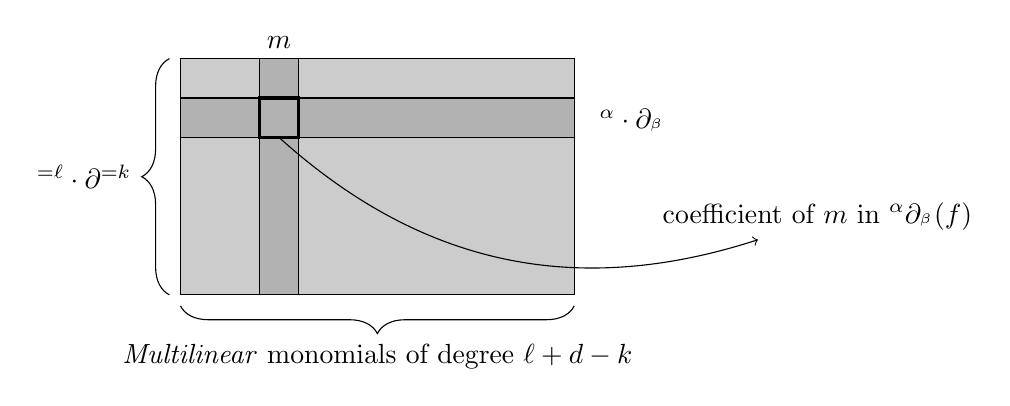
\begin{tikzpicture}
\draw[fill=black!20] (0,0) rectangle (5,3);

\draw[decorate,decoration={brace,amplitude=10pt,raise=4pt},yshift=0pt]
(0,0) -- (0,3);
\node[anchor=east] at (-0.5,1.5) {$\vecx^{=\ell} \cdot \partial^{=k}$};
\draw[decorate,decoration={brace,amplitude=10pt,mirror, raise=4pt},yshift=0pt] 
(0,0) -- (5,0);
\node[anchor=north] at (2.5,-0.5) {\emph{Multilinear} monomials of degree $\ell + d - k$};

\draw[fill=black!30] (1,0) rectangle (1.5,3);
\node at (1.25,3.2) {$m$};

\draw[fill=black!30] (0,2) rectangle (5,2.5);
\node[anchor=west] at (5.2,2.2) {$\vecx^{\alpha} \cdot \partial_{\vecx^\beta}$};

\draw[very thick] (1,2) rectangle (1.5,2.5);

\node[anchor=west] at (6,1) {coefficient of $m$ in $\vecx^\alpha \partial_{\vecx^\beta}(f)$}
edge[<-,bend left] (1.25,2);
\end{tikzpicture}

One can think of this as a sub-matrix for the shifted partial derivatives obtained by throwing out the columns corresponding to non-multilinear monomials.

This measure was used to prove lower bounds on the \emph{total size} of homogeneous depth four circuits (with no bottom fan-in restrictions), unlike the previous setting which was a top fan-in lower bound. But the following is an important note to bear in mind:
\begin{quote}
Projected shifted partial derivatives is designed to prove lower bounds on the top fan-in of homogeneous depth four circuits with \emph{low bottom support size}. 
\end{quote}
It so happens that any homogeneous depth four circuit of small total size can be reduced to a depth four circuit of small bottom support size. But this distinction is important and should be stressed. 

\subsection{Depth four circuits of low bottom support size}

Let $f = Q_1 \cdots Q_a$ with $d = \deg(f)$ and suppose all the monomials of any $Q_i$ depend on just $r$ variables.
There are two important observations made to prove the upper bound of the complexity measure on such circuits.

\begin{observation*}[Non-multiquadratic terms do not contribute]
Let $g$ be a polynomial such that every monomial of $g$ is divisible by some $x_i^3$, or in other words each monomial of $g$ is \emph{non-multiquadratic}. Then for an $k,\ell$, we have $\CM{PSD}_{k,\ell}(g) = 0$. 
\end{observation*}

\begin{observation*}[Decomposition of low support size products]
Let $f = Q_1 \cdots Q_a$ be a polynomial of degree $d$ such that all monomials of any $Q_i$ depends on at most $t$ variables. Then $f$ can be expressed as
\[
f \spaced{=} Q_1'\cdots Q_a' \spaced{+} g
\]
where $\deg(Q_i') \leq 2r$ for all $i$, and every monomial of $g$ is non-multiquadratic.
\end{observation*}

Therefore, we have
\[
\CM{PSD}_{k,\ell}(Q_1\cdots Q_a) = \CM{PSD}_{k,\ell}(Q_1'\cdots Q_a')
\]
and the RHS is a low bottom degree product. Thus similar to the upper bound for shifted partial derivatives, bearing in mind that we only care about multilinear monomials, one can easily show the following.

\begin{lemma*}[Upper bound for low bottom support size circuits, \autoref{lem:upper-bound-low-supp}]
Let $f = Q_1\cdots Q_a$ be an $n$-variate degree $d$ polynomial with each $Q_i$ a sum of monomials depending on at most $r$ variables. Then for any $k,\ell$ with $\ell + kr\leq \frac{n}{2}$, 
\[
\CM{PSD}_{k,\ell}(f) \spaced{\leq} \binom{(2d/r) + k}{k} \cdot \binom{n}{\ell + kr}
\]
\end{lemma*}

For a very delicate range of parameters, we have a very similar behaviour of the measure on the standard polynomials. 

\[
\CM{PSD}_{k,\ell}(Q_1\cdots Q_a) \ll \CM{PSD}_{k,\ell}(\IMM) \ll \CM{PSD}_{k,\ell}(\NW) \approx \text{Maximum possible}.
\]

In the right range of parameters, this gives an $n^{\Omega(d/t)}$ lower bound on the top fan-in of any homogeneous depth four circuit of bottom support size bounded by $t$ that computes $\NW$ or $\IMM$. 

The calculations involved are quite delicate but it would be useful to just keep the case of $\NW$ in mind as the full calculations were described in \autoref{sec:KS-leading-monomial-approach}. But a couple of thing to keep in mind is that the calculations for $\NW_{d,m,e}$ work over any field but as long as $m^e$ roughly equal to $2^d$ (the precise constraints are explicit described in \autoref{sec:KS-leading-monomial-approach}). \\

So far, this only addresses depth four circuits of small bottom support size. In order to reduce the general setting of homogeneous depth four circuits to this case, there is one additional trick employed. 

\subsection{Reducing  to depth four circuits of low bottom support size}

The key observation here is that if we have a depth four circuit of small size, then the number of distinct monomials computed at the layer closest to the leaves is bounded by the size of the circuit.
As a concrete instance, say we have a depth four circuit of size $s = n^{(0.1) \sqrt{d}}$.
We shall now pick a \emph{lot} of variables at random and set them to zero or to be more precise we shall set each variable to $0$ independently with probability $1 - \frac{1}{n^{0.2}}$. With very high probability, we would now be left with about $n^{0.8}$ variables but the resulting circuit remains homogeneous as setting variables to zero maintains homogeneity. 

However, if $m$ is a monomial that depends on $\sqrt{d}$ or more variables, the probability that this monomials survives this random restriction is at most $\frac{1}{n^{(0.2) \sqrt{d}}}$. Thus, even if we union bound over all monomials present in the depth four circuit of size $n^{(0.1)\sqrt{d}}$ we get
that the probability that some monomial of support $\sqrt{d}$ or more survives this process is at most $\frac{1}{n^{(0.1)\sqrt{d}}} = o(1)$. Thus, almost surely, the resulting circuit is now a homogeneous depth four circuit with bottom support size at most $\sqrt{d}$. \\

This however complicates the other side of the argument where we now need to find a polynomial $P$ such that \emph{even after a random restriction $\rho$ is applied on $P$}, we must have $\CM{PSD}_{k,\ell}(\rho(P))$ to be large. This is extremely non-trivial to see if $\NW$ or $\IMM$ are so robust. Fortunately, there is a hack that allows us to circumvent this at the cost of making the polynomial uglier. 

\begin{lemma*}[Linear blow-up trick to handle random restrictions, \autoref{lem:lin-transform-trick}]
Let $\rho$ be a random restriction that sets each variable to zero independently with probability $1 - \alpha$. 
For any polynomial $P(x_1,\dots x_n)$, define $P \circ \mathrm{Lin}_\alpha$ as
\[
P \circ \mathrm{Lin}_\alpha \spaced{=} P\inparen{\sum_{i=1}^t y_{1i}, \cdots, \sum_{i=1}^t y_{nt}}\quad \text{where $t = \inparen{\frac{1}{\alpha}} n \log n$}
\]
Then, $\rho(f \circ \mathrm{Lin}_\alpha)$ has $f$ as a projection with probability $1 - 1/2^{n}$. 
\end{lemma*}

Basically, we replace each variable in $\NW$ by a sum of $t$ new distinct variables where $t = (1/\alpha) \log n$. The point is that, if a variable is kept alive with probability $\alpha$, then with very high probability, one of the $t$ variables $\set{y_{ij}}_{j\in [t]}$ will be kept alive for each $x_i$. Hence, there is a copy of $\NW_{d,m,e}$ sitting inside $\rho(\NW_{d,m,e} \circ \mathrm{Lin}_\alpha)$ with very high probability. 

Therefore, if we assume on the contrary that $C$ is a homogeneous depth four circuit of size $n^{(0.1)\sqrt{d}}$ computing $\NW_{d,m,e} \circ \mathrm{Lin}_\alpha$, then there is a homogeneous circuit $C'$ with size at most $n^{(0.1)\sqrt{d}}$ and bottom support size at most $\sqrt{d}$ that computes $\NW_{d,m,e}$. But since we already have a lower bound for homogeneous depth four circuits of low bottom support size computing $\NW_{d,m,e}$, we get a contradiction. \\

Hopefully this would give the readers a rough description of the main observations. But to really understand them, one \emph{has} to work out the calculations in \autoref{sec:KS-leading-monomial-approach} at least once to get a better grip of how these parameters interact. We now move on to some other models for which projected shifted partials, or variants of it, can again be employed. 


%%% Local Variables:
%%% mode: latex
%%% TeX-master: "fancymain"
%%% End:


\chapter{Evaluation perspective on projected shifted partial derivatives}

The measure used in the lower bounds of Kayal, Limaye, Saha, Srinivasan~\cite{KLSS} and Kumar, Saraf~\cite{KS14} was the dimension of projected shifted partials.
As seen in that chapter, the calculations are extremely delicate.
In this chapter, we shall some slight modifications of this measure that is in a sense more \emph{algebraic} and hence useful in other lower bounds. 

\section{Coefficients vs evaluations}

For a moment, let us revisit the lower bounds of Nisan and Wigderson~\cite{nw1997}. The measure studied for the class of homogeneous depth-$3$ circuits in \autoref{thm:low-rank-sps-lb} was the dimension of partial derivatives. 
\[
\CM{NW}_k(f) \spaced{:=} \dim\set{\partial^{=k}(f)}
\]
More precisely, we interpret any element of $\partial^{=k}(f)$ as a long vector of coefficients and look at the dimension of this collection of vectors. That is, $\CM{NW}_k(f)$ is the rank of the following matrix. 

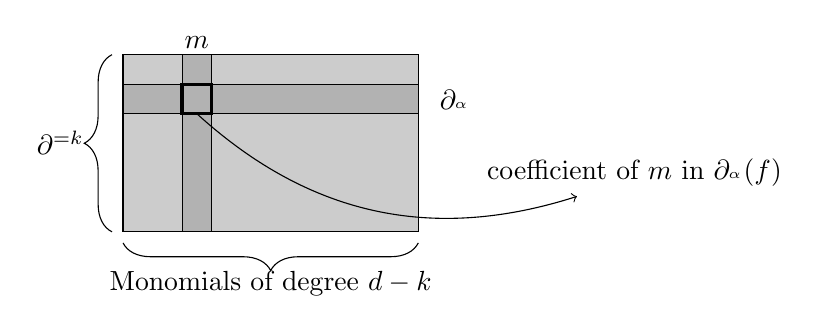
\begin{tikzpicture}[scale=0.75]
\draw[fill=black!20] (0,0) rectangle (5,3);

\draw[decorate,decoration={brace,amplitude=10pt,raise=4pt},yshift=0pt]
(0,0) -- (0,3);
\node[anchor=east] at (-0.5,1.5) {$\partial^{=k}$};
\draw[decorate,decoration={brace,amplitude=10pt,mirror, raise=4pt},yshift=0pt] 
(0,0) -- (5,0);
\node[anchor=north] at (2.5,-0.5) {Monomials of degree $d - k$};

\draw[fill=black!30] (1,0) rectangle (1.5,3);
\node at (1.25,3.2) {$m$};

\draw[fill=black!30] (0,2) rectangle (5,2.5);
\node[anchor=west] at (5.2,2.2) {$\partial_{\vecx^\alpha}$};

\draw[very thick] (1,2) rectangle (1.5,2.5);

\node[anchor=west] at (6,1) {coefficient of $m$ in $\partial_{\vecx^\alpha}(f)$}
edge[<-,bend left] (1.25,2);
\end{tikzpicture}

Grigoriev and Karpinski~\cite{grigoriev98}, for their lower bound for $\SPS$ circuits over finite fields instead looked at the dual \emph{evaluation perspective} by studying a matrix of the form

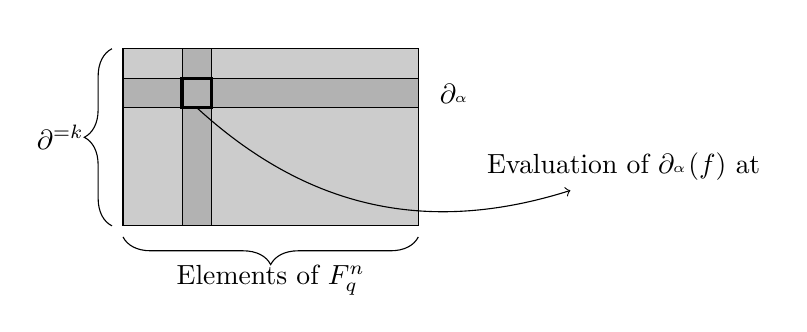
\begin{tikzpicture}[scale=0.75]
\draw[fill=black!20] (0,0) rectangle (5,3);

\draw[decorate,decoration={brace,amplitude=10pt,raise=4pt},yshift=0pt]
(0,0) -- (0,3);
\node[anchor=east] at (-0.5,1.5) {$\partial^{=k}$};
\draw[decorate,decoration={brace,amplitude=10pt,mirror, raise=4pt},yshift=0pt] 
(0,0) -- (5,0);
\node[anchor=north] at (2.5,-0.5) {Elements of $F_q^n$};

\draw[fill=black!30] (1,0) rectangle (1.5,3);
\node at (1.25,3.2) {$\veca$};

\draw[fill=black!30] (0,2) rectangle (5,2.5);
\node[anchor=west] at (5.2,2.2) {$\partial_{\vecx^\alpha}$};

\draw[very thick] (1,2) rectangle (1.5,2.5);

\node[anchor=west] at (6,1) {Evaluation of $\partial_{\vecx^\alpha}(f)$ at $\veca$}
edge[<-,bend left] (1.25,2);
\end{tikzpicture}

As seen in \autoref{chap:GK}, the measure $\CM{GK}_k$ was the rank of the above matrix (with a few columns removed).
Intuitively, we expect that if the rank of the \emph{coefficient} matrix is large, then the rank of the \emph{evaluation} matrix should also be large.
Sometimes, the evaluation perspective allows us to handle the circuit model better.
In a way, the proof of Grigoriev and Karpinski~\cite{grigoriev98} can be thought of as a formalization of this intuition for $\SPS$ circuits.
\\

A similar perspective can also be adopted for the dimension of shifted partial derivatives.
For the dimension of projected shifted partials however, this connection is not that clean.
Roughly speaking, throwing away non-multilinear monomials changes the evaluations of the shifted partials at points.
Formally, the multilinear projection of a polynomial $f$ can be interpreted as looking at the residue of $f \bmod \setdef{x_i^2}{i\in [n]}$, that is just replacing any $x_i^2$ by zero.
However this reduction does not work well with evaluations as $f(\veca)$ could be different from $(f \bmod \setdef{x_i^2}{i\in [n]})(\veca)$ for each $\veca \in \F^n$. 

Let us turn the question around and ask if we wish to understand the rank of the following matrix

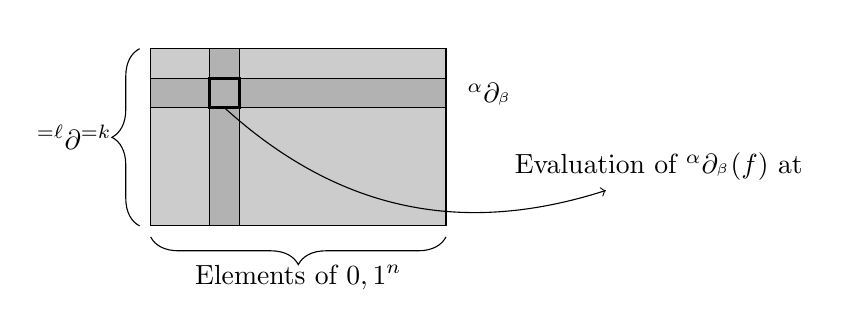
\begin{tikzpicture}[scale=0.75]
\draw[fill=black!20] (0,0) rectangle (5,3);

\draw[decorate,decoration={brace,amplitude=10pt,raise=4pt},yshift=0pt]
(0,0) -- (0,3);
\node[anchor=east] at (-0.5,1.5) {$\vecx^{=\ell}\partial^{=k}$};
\draw[decorate,decoration={brace,amplitude=10pt,mirror, raise=4pt},yshift=0pt] 
(0,0) -- (5,0);
\node[anchor=north] at (2.5,-0.5) {Elements of $\set{0,1}^n$};

\draw[fill=black!30] (1,0) rectangle (1.5,3);
\node at (1.25,3.2) {$\veca$};

\draw[fill=black!30] (0,2) rectangle (5,2.5);
\node[anchor=west] at (5.2,2.2) {$\vecx^{\alpha}\partial_{\vecx^\beta}$};

\draw[very thick] (1,2) rectangle (1.5,2.5);

\node[anchor=west] at (6,1) {Evaluation of $\vecx^\alpha\partial_{\vecx^\beta}(f)$ at $\veca$}
edge[<-,bend left] (1.25,2);
\end{tikzpicture}

\noindent
what is the \emph{coefficient} analogue of this measure?
Turns out, the answer is a different notion of projected shifted partial derivatives where the projection is not modulo $\setdef{x_i^2}{i\in [n]}$ but instead modulo $\setdef{x_i^2 - x_i}{i\in [n]}$.
It should be intuitively clear that as long as we are only interested in evaluations on $\set{0,1}^n$, the evaluation of  $f \bmod \setdef{x_i^2 - x_i}{i\in [n]}$ at $\veca\in \set{0,1}^n$ yields the same  as $f(\veca)$. 

What can we say about this modification of projected shifted partial derivatives? Is this also a measure that can give the homogeneous depth-$4$ lower bounds studied in \autoref{chap:d4hom}? Turns out the answer is indeed yes, and this perspective also allows one to generalize the lower bounds to homogeneous depth-$5$ circuits over finite fields (similar to Grigoriev-Karpinski) by Kumar and Saptharishi~\cite{KumarSapt15}. 

\section{Projected shifted partials via $\setdef{x_i^2-x_i}{i\in [n]}$}

The following definition is a little more general but would be useful later in this chapter. But for now, it would be useful to just consider $\mathcal{I} = \inangle{x_i^2 - x_i \;:\; i\in [n]}$. 

 \begin{definition}[PSDs with respect to $\mathcal{I}$] \label{defn:PSPD-ideal}
The \emph{projected shifted partial derivatives with respect to $\mathcal{I}$} for a polynomial $f$, denoted by $\Gamma_{k,\ell,\mathcal{I}}(f)$, is defined as 
\[
\Gamma^{\mathrm{PSD}}_{k,\ell,\mathcal{I}}(f) \spaced{:=} \dim \set{\inparen{\vecx^{=\ell} \cdot \partial^{=k}(f)} \bmod \mathcal{I}}.\qedhere
\]
\end{definition}
\noindent
In the setting where $\mathcal{I} = \inangle{x_i^2 - x_i\;:\; i\in [n]}$, every polynomial $f$, there is a unique multilinear polynomial $g$ for which $f = g \bmod \mathcal{I}$ and we shall refer to this $g$ by $f \bmod \mathcal{I}$. Thus, $\Gamma_{k,\ell,\mathcal{I}}(f)$ is the rank of the following matrix:

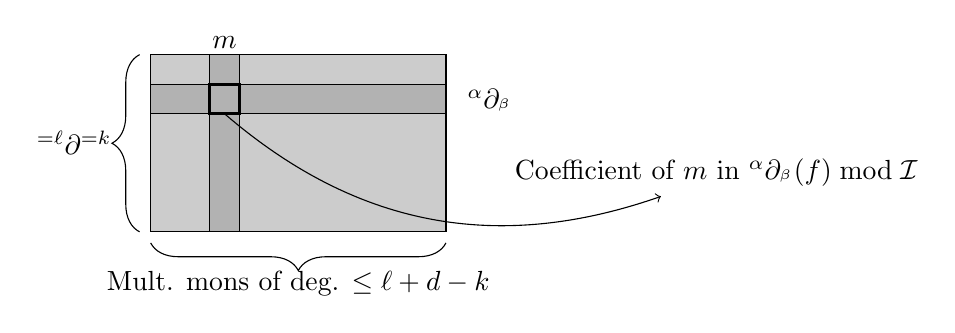
\begin{tikzpicture}[scale=0.75]
\draw[fill=black!20] (0,0) rectangle (5,3);

\draw[decorate,decoration={brace,amplitude=10pt,raise=4pt},yshift=0pt]
(0,0) -- (0,3);
\node[anchor=east] at (-0.5,1.5) {$\vecx^{=\ell}\partial^{=k}$};
\draw[decorate,decoration={brace,amplitude=10pt,mirror, raise=4pt},yshift=0pt] 
(0,0) -- (5,0);
\node[anchor=north] at (2.5,-0.5) {Mult. mons of deg. $\leq \ell + d - k$};

\draw[fill=black!30] (1,0) rectangle (1.5,3);
\node at (1.25,3.2) {$m$};

\draw[fill=black!30] (0,2) rectangle (5,2.5);
\node[anchor=west] at (5.2,2.2) {$\vecx^{\alpha}\partial_{\vecx^\beta}$};

\draw[very thick] (1,2) rectangle (1.5,2.5);

\node[anchor=west] at (6,1) {Coefficient of $m$ in $\vecx^\alpha\partial_{\vecx^\beta}(f) \bmod \mathcal{I}$}
edge[<-,bend left] (1.25,2);
\end{tikzpicture}

\noindent In \autoref{defn:PSPD}, we are essentially working with
$\mathcal{I} = \inangle{x_i^2 \;:\; i\in [n]}$ but working modulo other ideals is at times more useful.
In fact, there is a fairly large class of ideals $\mathcal{I}$ for which $f \bmod \mathcal{I}$ has a unique multilinear representative. But to make it applicable for lower bounds for homogeneous depth-$4$ circuits, we will need a mechanism to transform a ``low support polynomial'' to a ``low degree polynomial''. 

\begin{definition}[Support-to-degree ideals]\label{defn:supp-to-degree-ideal}
An ideal $\mathcal{I}$ is said to be a \emph{support-to-degree} ideal if there exist linear polynomials $\ell_1, \cdots, \ell_n$ such that
\[
\mathcal{I} \spaced{=} \inangle{x_i^2 - \ell_i(x_i) \;:\; i\in [n]}. \qedhere
\]
\end{definition}

\begin{observation}\label{obs:support-redn}
For any polynomial $f$ and a support-to-degree ideal $\mathcal{I}$, there is a unique multilinear polynomial $g$ such that $f = g \bmod\mathcal{I}$. 

Furthermore, if $f$ is a polynomial such that every monomial in $f$ depends on at most $r$ variables, then the unique multilinear polynomial $g = f \bmod\mathcal{I}$ in fact has degree at most $r$. 
\end{observation}
\begin{proof}
The proof follows immediately by repeatedly replacing $x_i^2$ by $\ell_i(x_i)$.
\end{proof}

As mentioned before, we would need the above more general definition in a later lower bound but for now it would help to just keep ideals such as $\inangle{x_i^2\;:\;i\in [n]}$ or $\inangle{x_i^2 - x_i\;:\;i\in [n]}$ in mind. \\

In order to check if \autoref{defn:PSPD-ideal} is a measure useful for homogeneous depth-$4$ circuits, we need to show two things --- (1) the measure is small for a small homogeneous depth-$4$ circuit (of low bottom support), and (2) the measure is large for an explicit polynomial.
These together would imply the practicability of dimension of projected shifted partials with respect to an arbitrary support-to-degree ideal.

The second claim would be easier to prove so let us address that first. 

\begin{lemma}[PSD wrt $\mathcal{I}$ for homogeneous polynomials]\label{lem:PSD-I-lowerbound} Let $f$ be any homogeneous polynomial of degree $d$. For any choice of $k,\ell$ and any support-to-degree ideal $\mathcal{I}$, we have
\[
\Gamma^{\mathrm{PSD}}_{k,\ell,\mathcal{I}}(f) \spaced{\geq} \Gamma^{\mathrm{PSD}}_{k,\ell}(f).
\]
\end{lemma}
\begin{proof}
  Let $g \in \vecx^{=\ell} \cdot \partial^{=k}(f)$.
The main difference between $g \bmod \inangle{x_i^2\;:\; i \in [n]}$ and $g \bmod\mathcal{I}$ is just that the first projection just zeros out any non-multilinear monomial of degree $\ell + d -k$ whereas $g \bmod\mathcal{I}$ reduces non-multilinear monomials to lower degree monomials.
Hence, $g \bmod\inangle{x_i^2\;:\; i \in [n]}$ is just $g \bmod \mathcal{I}$ but just restricted to the multilinear monomials of degree $\ell + d - k$. 
Thus it follows that the rank of $\inparen{\vecx^{=\ell} \partial^{=k}g} \bmod\mathcal{I}$ is lower bounded by the rank of $\inparen{\vecx^{=\ell} \partial^{=k}g} \bmod\inangle{x_i^2\;:\; i \in [n]}$.
\end{proof}

We now want to show that if $C$ is a homogeneous depth-$4$ circuit with bottom support at most $r = O(\sqrt{d})$, then we can give a good upper bound for $\Gamma^{\mathrm{PSD}}_{k,\ell,\mathcal{I}}(C)$. 

\begin{lemma}[PSD wrt $\mathcal{I}$ for a hom. $\SPSP$ circuit]\label{lem:PSPD-I-upperbound} Let $C$ be a homogeneous $\SPSP$ computing an $n$-variate degree $d$ polynomial of top fan-in $s$ and bottom support bounded by $r$. Then for any choice of $k,\ell$ and any support-to-degree ideal $\mathcal{I}$ we have
\[
\Gamma^{\mathrm{PSD}}_{k,\ell,\mathcal{I}} \spaced{\leq} s \cdot \binom{3(d/r) + 1}{k} \cdot \binom{n}{\ell + kr}
\]
\end{lemma}
\begin{proof}
  Let us consider a single summand $T = Q_1 \cdots Q_m$ of $C$.
We shall partition this set into those polynomials $Q_1,\cdots, Q_a$ of degree at most $r$, and polynomials $Q_1',\cdots, Q_b'$ of degree more than $r$. By homogeneity of $C$, we know that $b \leq d/r$. Since some of the $Q_i$s could have very small degree, $a$ could potentially be as large as $d$. To handle this, if we find any $Q_i$ and $Q_j$ both of degree at most $r/2$, we shall replace them by their product. This ensures that all $Q_i$s have degree more than $r/2$ except perhaps one. Hence, (reusing some symbols) we can write $T$ as
\[
T \spaced{=} \tilde{Q}_1 \cdots \tilde{Q}_a \;\cdot\; Q_1' \cdots Q_b'
\]
where each $a \leq 2(d/r) + 1$, $b \leq (d/r)$, each $Q_i$ has degree at most $r$ and every monomial in a $Q_i'$ depends on at most $r$ variables. For brevity, we shall use the notation $\tilde{Q}_A$ to denote $\prod_{i\in A} \tilde{Q}_i$, and similarly $Q_B'$ to denote $\prod_{i\in B} Q_i'$. 

Let $\partial_{\vecx^\alpha}(T)$ be a $k$-th order partial derivative of $T$. By the chain rule of differentiation,
\begin{eqnarray*}
\partial_{\vecx^\alpha}(T) & \in & \mathrm{span}\setdef{ \partial_{\vecx^\beta}(\tilde{Q}_A) \cdot \partial_{\vecx^\gamma}(Q_B') \cdot \tilde{Q}_{\overline{A}} \cdot Q_{\overline{B}}'}{\begin{array}{c} \vecx^{\alpha} = \vecx^\beta \cdot \vecx^\gamma\\ |A| + |B| \leq k  \end{array}}\\
 & \subseteq & \mathrm{span}\setdef{ \vecx^{\leq k(r - 1)} \cdot \partial_{\vecx^\gamma}(Q_B') \cdot \tilde{Q}_{\overline{A}} \cdot Q_{\overline{B}}'}{\begin{array}{c} \vecx^{\alpha} = \vecx^\beta \cdot \vecx^\gamma\\ |A| + |B| \leq k  \end{array}}\\
\implies \vecx^{=\ell} \cdot \partial_{\vecx^\alpha}(T) & \subseteq & \mathrm{span}\setdef{ \vecx^{\leq \ell + k(r - 1)} \cdot \partial_{\vecx^\gamma}(Q_B') \cdot \tilde{Q}_{\overline{A}} \cdot Q_{\overline{B}}'}{\begin{array}{c} \vecx^{\alpha} = \vecx^\beta \cdot \vecx^\gamma\\ |A| + |B| \leq k  \end{array}}
\end{eqnarray*}
We now have to look at $\vecx^{=\ell} \cdot \partial_{\vecx^\alpha}(T) \bmod\mathcal{I}$ and for that notice that $Q_B'$ is a product of polynomials of low-support, that is each monomial $Q_i'$ depends on at most $\sqrt{d}$ variables. Therefore, by applying the product rule on $\partial_{\vecx^{\gamma}}(Q_B')$, we know that this can be written as a linear combination of products of low-support polynomials. By \autoref{obs:support-redn}, every polynomial $f$ of support at most $r$ there is a unique multilinear polynomial $g = f\bmod \mathcal{I}$ of degree at most $r$. Hence, we get that
\begin{eqnarray*}
\vecx^{=\ell} \cdot \partial_{\vecx^\alpha}(T) \bmod\mathcal{I} & \subseteq& \mathrm{span}\setdef{ \vecx^{\leq \ell + k(r - 1)} \cdot \vecx^{\leq k(r)} \cdot \tilde{Q}_{\overline{A}} \cdot Q_{\overline{B}}'}{\begin{array}{c} \vecx^{\alpha} = \vecx^\beta \cdot \vecx^\gamma\\ |A| + |B| \leq k  \end{array}} \bmod \mathcal{I}\\
& = & \mathrm{span}\setdef{ \vecx^{\leq \ell + kr} \cdot \tilde{Q}_{\overline{A}} \cdot Q_{\overline{B}}'}{\begin{array}{c} \vecx^{\alpha} = \vecx^\beta \cdot \vecx^\gamma\\ |A| + |B| \leq k  \end{array}} \bmod \mathcal{I}.
\end{eqnarray*}
\noindent
Therefore, an upper bound on $\set{\vecx^{=\ell} \partial^{=k}(T) \bmod \mathcal{I}}$ is 
\[
\binom{2(d/r) + 1 + (d/r)}{k} \cdot \binom{n}{\ell + kr} \cdot n
\]
\noindent
Hence, if $C = T_1 + \cdots + T_s$, then by sub-additivity we get
\[
\Gamma^{\mathrm{PSD}}_{k,\ell,\mathcal{I}}(C) \spaced{=} s \cdot \binom{3(d/r) + 1}{k} \cdot \binom{n}{\ell + kr} \cdot n.\qedhere
\]
\end{proof}

\noindent
The bound above is almost the same as in \autoref{lem:upper-bound-low-supp} and the difference is only $\exp(O(d/r))$ due to the first binomial coefficient above. \autoref{lem:PSD-I-lowerbound} and 
\autoref{lem:d4hom-goldilocks-LB} yields a lower bound for $\Gamma^{\mathrm{PSD}}_{k,\ell,\mathcal{I}}(\NW)$ as well. \\

What did we gain by looking at $\Gamma^{\mathrm{PSD}}_{k,\ell,\mathcal{I}}$ at the end of all this?
The key point is makes it easier to look at the evaluation perspective for such measures when the ideal $\mathcal{I}$ \emph{cooperates} with the evaluation operation.
A concrete instance of this was the lower bound by Kumar and Saptharishi~\cite{KumarSapt15} for homogeneous depth five circuits over finite fields.

\section{Lower bounds for depth five circuits over finite fields}

The plan would be to combine the ideas from the lower bound of Grigoriev and Karpinski \cite{grigoriev98} (discussed in \autoref{chap:GK}) with the above perspective of projected shifted partial derivatives.
The main theorem of this chapter would be the result of Kumar and Saptharishi~\cite{KumarSapt15}.

\begin{theorem}[\cite{KumarSapt15}]\label{thm:Kumar-Sapt-d5-thm}
Consider $\NW_{d,m,e}$ for some suitable choice of parameter. For any finite field $\F_q$, any homogeneous depth-$5$ circuit computing $\NW_{d,m,e}$ must be of size $\exp(\Omega_q(\sqrt{d}))$. 
\end{theorem}

\noindent 
The plan that one could adopt is the following. 
\begin{enumerate}
\itemsep 0pt
\item\label{item:PSPD-1} Take the measure to be $\Gamma^{\mathrm{PSD}}_{k,\ell,\mathcal{I}}$ where $\mathcal{I} = \inangle{x_i^q - x_i \;:\; i\in [n]}$, which is the \emph{evaluation perspective} of the shifted partial derivatives on $\F_q^n$.
\item\label{item:PSPD-2} As an analogue of ``support'' for the hom. $\SPSP$ lower bounds, we shall look at look at ``rank'' of products of linear polynomials computed by the bottom two layers of the circuit. 
\item\label{item:PSPD-3} Intuitively, any term of rank at most $r$ should be essentially behave like a term of degree at most $(q-1)r$, as $\mathcal{I}$ reduces any variable of exponent $q$ or above. 

Hence, the ``low-rank'' part of the circuit (only considering terms of rank at most $\sqrt{d}$) should behave like a homogeneous $\SPSP^{[q\sqrt{d}]}$ circuit, for which we can upper bound the measure in a similar fashion. 
\item\label{item:PSPD-4} To eliminate the ``high-rank'' products of linear polynomials, just as in the lower bound of Grigoriev and Karpinski \cite{grigoriev98} (as discussed in \autoref{chap:GK}), these ``high-rank'' gates are zero on almost all evaluations. 
Therefore, we can modify our measure to not look at all evaluations on $\F_q^n$ but instead at $\F_q^n \setminus \mathcal{E}$ where $\mathcal{E}$ a tiny subset of $\F_q^n$ (of about $\exp(-\sqrt{d}) \cdot q^n$ size). 

\item\label{item:PSPD-5} For the hard polynomial $\NW_{d,m,e}$, hopefully the measure continues to remain large even under the evaluation perspective on $\F_q^n \setminus \mathcal{E}$. 
\end{enumerate}

This is certainly a legitimate plan but the difficulty is in proving~\autoref{item:PSPD-5}.
The calculations for the projected shifted partials were intricate enough, and it unclear how to convert those to the evaluation perspective with a few columns removed.
Furthermore, it is important to keep the rough ballpark of parameters in mind.
If we are hoping to have parameters for $k$ and $\ell$ similar to those in \autoref{chap:d4hom}, then we are dealing with matrices with roughly $2^n \cdot \exp(O(\sqrt{d}\log n))$ rows (indexed by derivatives of order $k = O(\sqrt{d})$ and shifts of order $\ell \approx n/2$) but close to $q^n$ columns.
It would have been fine if we actually had all $q^n$ columns but we have to instead work with evaluations only on $\F_q^n \setminus \mathcal{E}$ for a set $\mathcal{E}$ of size $\exp{(-\sqrt{d})} \cdot q^n \gg 2^n$. 

In \autoref{chap:GK}, we used the property that any linear combination of determinantal minors have many non-zero evaluations. Such a statement is simply false for this setting as we are dealing with polynomials that are multiplied by monomials of degree $\approx n/2$ and are hence going to be zero at many evaluations. Therefore, one needs a different strategy. \\

{\bf Idea 1:} Since we are dealing with a matrix of evaluations, it can be naturally written as a product of a ``coefficient matrix'' and a ``Vandermonde matrix''.

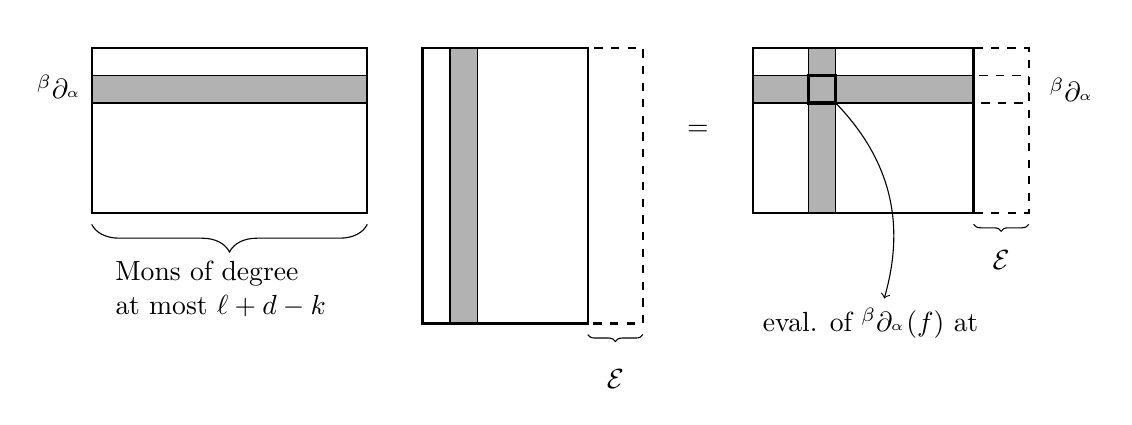
\begin{tikzpicture}[scale=0.7]
  \draw[decorate,decoration={brace,amplitude=10pt,mirror, raise=4pt},yshift=0pt] 
  (0,0) -- (5,0);
  \node[anchor=north,text width=5cm] at (4,-0.7) {Mons of degree\\at most $\ell + d - k$};
  \draw[fill=black!30] (0,2) rectangle (5,2.5);
  \draw[dashed,thick] (9,-2) rectangle (10,3);
  \draw[decorate,decoration={brace,mirror, raise=4pt},yshift=0pt] 
  (9,-2) -- (10,-2);
  \node at (9.5,-3) {$\mathcal{E}$};
  \draw[fill=black!30] (6.5,3) rectangle (7,-2);
  \node at (6.75,3.2) {$\veca$};
  \node[anchor=east] at (0,2.25) {$\vecx^{\beta}\partial_{\vecx^\alpha}$};
  \draw[thick] (6,-2) rectangle (9,3);
  \draw[thick] (0,0) rectangle (5,3);

  \begin{scope}[shift={(12,0)}]
  \node at (-1,1.5) {$=$};
  \draw[decorate,decoration={brace,mirror, raise=4pt},yshift=0pt] 
  (4,0) -- (5,0);
  \node[anchor=north] at (4.5,-0.5) {$\mathcal{E}$};
  
  \draw[fill=black!30] (1,0) rectangle (1.5,3);
  \node at (1.25,3.2) {$\veca$};
  
  \draw[fill=black!30] (0,2) rectangle (4,2.5);
  \draw[dashed] (4,2) rectangle (5,2.5);
  \node[anchor=west] at (5.2,2.2) {$\vecx^{\beta}\partial_{\vecx^\alpha}$};
  
  \draw[very thick] (1,2) rectangle (1.5,2.5);
  
  \node[anchor=west] at (0,-2) {eval. of $\vecx^{\beta}\partial_{\vecx^\alpha}(f)$ at $\veca$}
  edge[<-,bend right] (1.5,2);
  \draw[thick] (0,0) rectangle (4,3);
  \draw[dashed,thick] (4,0) rectangle (5,3);
  \end{scope}
\end{tikzpicture}

Formally, let $C$ be  a matrix with rows indexed by shifted partials and columns indexed by monomials of the right degree, so that each row of $C$ is just the coefficients of a shifted partial $\vecx^{\beta} \partial_{\vecx^\alpha}(f) \bmod \mathcal{I}$ listed down. Also, let $V$ be the evaluation matrix of the monomials where rows are indexed by monomials and columns indexed by points in $\F_q^n$. Then the product $C \cdot V$ is precisely the evaluation matrix of shifted partials modulo $\mathcal{I}$. Furthermore, discarding a set $\mathcal{E}$ of evaluations is just discarding the corresponding columns from $V$. 

In \autoref{chap:d4hom}, we essentially showed that the matrix $C$ for $\NW_{d,m,e}$ has pretty large row-rank.
Furthermore, it is easy to show that $V$ also has full-rank.
Since $\mathcal{E}$ is a fairly small set, we should expect $\tilde{V}$, which is $V$ with the columns indexed by $\mathcal{E}$ removed, to also have very large rank.
Can we therefore claim that $C \cdot \tilde{V}$ also has large rank?
In some sense, we  certainly can.

\begin{lemma}[Rank of products]\label{lem:rank-of-products}
For matrices $X \cdot Y = Z$, we always have that
\[
\rank(X) \spaced{\geq} \rank(Y) \;+\; \rank(Z) \;-\; (\mathrm{common\ dimension})
\]
where $\mathrm{common\ dimension}$ denotes the number of columns of $X$ or the number of rows of $Y$. 
\end{lemma}

Of course, if $\tilde{V}$ has full-rank then $\rank(M) = \rank(C)$.
The problem is that if we are forced to look at a subset of evaluations and hence $\tilde{V}$ may not be full rank.
When we are looking at all evaluations on $\F_q^n$, then the matrix $V$ and $\tilde{V}$ has much more $2^n$ rows as row indices would also involve non-multilinear monomials.
However $C$ just has $2^n$ rows and hence they could potentially all be in the left-kernel of $\tilde{V}$ thus making $C \cdot \tilde{V} = 0$.
Thus, we need a way of reducing the number of rows in $V$ to about $2^n$.
\\

{\bf Idea 2:} Do not consider evaluations on $\F_q^n$ but just evaluations on $\set{0,1}^n \subset \F_q^n$. \\

\noindent
That way, it is equivalent to reducing all polynomials $\mathcal{I} = \inangle{x_i^2 - x_i \;:\;i\in [n]}$ and hence the rows of $V$ (or columns of $C$) would be indexed by only multilinear monomials of degree at most $\ell+d-k$, which is the same regime as in \autoref{chap:d4hom}.
Hence, we can hope to use \autoref{lem:rank-of-products} to lower bound the measure for $\NW_{d,m,e}$.

The problem now becomes \autoref{item:PSPD-4}, the ``high rank'' gates.
Consider the high-rank term $(x_1 + 2) \cdots (x_n + 2)$ over say $\F_7$.
This term remains non-zero when we evaluate on any point in $\set{0,1}^n$.\\

{\bf Idea 3:} Do not consider evaluations on $\set{0,1}^n$ but rather on a \emph{shift} of $\set{0,1}^n$. \\

Picking a random point $\F_q^n$ can be thought of as first picking a point $\vecc \in \F_q^n$, and then picking a shift $\vecx \in \set{0,1}^n$ and returning $\vecc + \vecx$.
Therefore, if we have an event that is \emph{good} for a random point in $\F_q^n$, this also shows that there exists a $\vecc \in \F_q^n$ for which the event is \emph{good} for a random point in $\vecc + \set{0,1}^n$.

\begin{lemma}\label{lem:shift-of-hypercube-averaging}
Let $A$ be an function on $\F_q^n$ and suppose $\E_{\vecy \in \F_q^n}[A(\vecy)] \geq \delta$. Then, there exists a point $\vecc \in \F_q^n$ such that 
\[
\E\limits_{\vecy \in \vecc + \set{0,1}^n}[A(\vecy)] \spaced{\geq} \delta
\]
\end{lemma}

In this setting, if the event is the vanishing of all high-rank gates, we now have that there exists a \emph{translate of a hypercube} $\vecc + \set{0,1}^n$ such all high rank gates vanish on most points in this translate of a hypercube.

We are now back to~\autoref{item:PSPD-5}, lower bounding the rank of the evaluation matrix for $\NW_{d,m,e}$.
Since we are only dealing with a translate of a hypercube, we can finding a support-to-degree ideal $\mathcal{I}$ that respects evaluations on $\vecc + \set{0,1}^n$.

\begin{lemma}[\cite{KumarSapt15} Multilinearization for translate of hypercubes]\label{lem:multilinearization-translate}
  Let $\vecc + \set{0,1}^n$.
Then there exists a support-to-degree ideal $\mathcal{I}$ such that every polynomial $f(\vecx) \in \F_q^n$ has a unique multilinear representative $g$ with $\deg(g) \leq \deg(f)$ that agrees with $f$ on $\vecc + \set{0,1}^n$.
\end{lemma}
\begin{proof}
  Since each $x_i$ can only take values $c_i$ or $c_i + 1$, it suffices to replace each $x_i^2$ by either $c_i^2$ or $(c_i + 1)^2$ depending on the value of $x_i$.
It is easy to find a linear polynomial $\ell_i$ such that $\ell_i(c_i) = c_i^2$ and $\ell_i(c_i+1) = (c_i+1)^2$ --- a simple calculation yields $\ell_i(x) = c_i^2 + (x - c_i)(2c_i + 1)$.
Hence, if we define $\mathcal{I}$ to be
\[
\mathcal{I} \spaced{=} \setdef{x_i^2 - c_i^2 - (x_i - c_i)(2c_i + 1)}{i\in [n]},
\]
clearly this is a support-to-degree ideal (\autoref{defn:supp-to-degree-ideal}) and by definition does not alter the evaluation on $\vecc + \set{0,1}^n$. 
\end{proof}

With this multilinearization lemma, the coefficient matrix $C$ has columns indexed by just multilinear monomials of degree at most $\ell + d - k$ which makes the dimensions $C$ more balanced. 

These are the main ideas that go into the proof of Kumar and Saptharishi \cite{KumarSapt15} and from here on is just setting the right parameters etc.
The rest of the exposition will leave a lot of the proofs as exercises to the readers as the main intuitions have been exposed.

\subsubsection*{The formal measure}

For a set $\mathcal{A} \subseteq \F_q^n$, define the measure $\CM{KS}_{k,\ell,\mathcal{A}}$ as follows
\[
\CM{KS}_{k,\ell,\mathcal{A}}(f) \spaced{=} \rank \set{\inparen{\vecx^{= \ell} \cdot \partial^{=k}(f)  }_{\veca \in \mathcal{A}}}
\]
or in other words is the rank of the matrix where rows are indexed by shifts and partial derivatives, columns are indexed by elements $\mathcal{A}$ and the corresponding entry being the evaluation of the shifted partial derivative of $f$ at the point $\veca$.

\subsection{Upper bound for a homogeneous depth-$5$ circuit}

The upper bound would proceed in the following natural steps, similar to the discussion in \ref{chap:GK}. 

\begin{lemma}[\cite{KumarSapt15} Eliminating high-rank gates]
  Let $C$ be a homogeneous depth-$5$ circuit that computes an $n$-variate degree $d$ polynomial over $\F_q$.
Assume that $\mathrm{size}(C) \leq 2^{\sqrt{d}/100}$.
Let $\tau = q\sqrt{d}/6$ and $k = \tau / 2q^3 = O_q(\sqrt{d})$.
Then, there is a set $\mathcal{E}$ of size at most $\exp{-O(\sqrt{d})} \cdot q^n$ such that all products of linear polynomials of rank greater than $\tau$ that are computed by the bottom to layers of $C$ vanish on all of $\F_q^n \setminus \mathcal{E}$ with multiplicity at least $k$.
\end{lemma}
\begin{exercise}
Prove this. 
\end{exercise}


\begin{lemma}[\cite{KumarSapt15} Upper bound]\label{lem:PSPD-more-upper-bound-ckt}
Let $C$ be a homogeneous depth-$5$ circuit of size at most $2^{\sqrt{d}/100}$ that computes an $n$-variate degree $d$ polynomial over $\F_q$. Let $\tau, k, \mathcal{E}$ be as above. 
Then, for any $\mathcal{A} \subset \F_q^n \setminus \mathcal{E}$ that is contained in some $\vecc + \set{0,1}^n$, we have
\[
\CM{KS}_{k,\ell,\mathcal{A}}(C) \spaced{\leq} 2^{\sqrt{d}/100} \cdot \binom{\frac{4d}{\tau} + 1}{k} \cdot \binom{n}{\ell + k\tau q} \cdot \poly(n)
\]
\end{lemma}

This proof would proceed in a few steps. 

\begin{claim}
Consider the polynomial $C'$ which is obtained from $C$ by \emph{dropping all products of linear polynomials or rank at least $\tau$}. Then, by the choice of $\mathcal{A}$,
\[
\CM{KS}_{k,\ell,\mathcal{A}}(C) \spaced{=}\CM{KS}_{k,\ell,\mathcal{A}}(C')
\]
\end{claim}

\begin{claim}
  If $C'$ is a homogeneous depth-$5$ circuit with all products of linear forms having rank at most $\tau$, and if $\mathcal{A}$ is contained in some translate of a hypercube $\vecc + \set{0,1}^n$, then
\[
\CM{KS}_{k,\ell,\mathcal{A}}(C') \spaced{=} \mathrm{size}(C') \cdot \binom{\frac{4d}{\tau} + 1}{k} \cdot \binom{n}{\ell + k\tau q} \cdot \poly(n)
\]
\end{claim}

\begin{exercise}
Complete the proofs using \autoref{obs:support-redn} and \autoref{lem:multilinearization-translate}. 
\end{exercise}

\subsection{Lower bound for $\NW_{d,m,e}$}

As mentioned earlier, to lower bound the rank of the evaluation matrix we shall write this as $C \cdot V$ and use \autoref{lem:rank-of-products} to lower bound the rank.
The matrices $C$ and $V$ shall be the following:
\begin{quote}
{\bf The matrix $C$:}

Rows are indexed by shifted partials, columns are indexed by multilinear monomials of degree at most $\ell + d - k$, and the entry in $(\vecx^{\alpha} \cdot \partial_{\vecx^{\beta}} , m)$ is the coefficient of the monomial $m$ in the unique multilinear representative of $\vecx^{\alpha} \cdot \partial_{\vecx^{\beta}}(f) \bmod{\mathcal{I}}$ (\autoref{lem:multilinearization-translate}). 

{\bf The matrix $V({\mathcal{A}})$:} 

Rows are indexed by multilinear monomials of degree at most $\ell + d - k$, columns are indexed by points in $\mathcal{A}$, and the entry at $(m,\veca)$ is the evaluation of $m$ at $\veca$.
\end{quote}

We shall set parameters in $\NW_{d,m,e}$ as we had in \autoref{lem:d4hom-goldilocks-LB}, then by \autoref{lem:PSD-I-lowerbound}, we have the following bound for the rank of $C$.

\begin{eqnarray}
\rank(C) & \geq & \binom{n}{\ell} \cdot (1 + \epsilon)^{2d-2k} \cdot \exp(-O(\log^2 n))\nonumber\\
 & = & \binom{n}{\ell + d - k} \cdot \exp(-O(\log^2 n))\label{eqn:rank-C-lower-bound}
\end{eqnarray}

Moving on to the rank of $V(\mathcal{A})$.
Currently, $\mathcal{A}$ is contained in some translate $\vecc + \set{0,1}^n$.
The following observation allows us to instead look at subsets of $\set{0,1}^n$, which is easier to study.

\begin{observation} For any set $\mathcal{A}$ and a point $\vecc \in \F_q^n$, we have 
\[
\rank(V(\mathcal{A}) = \rank(V(\mathcal{A} - \vecc)). 
\]
\end{observation}
\begin{exercise}
Prove this. 
\end{exercise}

Due to this observation, we might as well assume that $\mathcal{A} \subset \set{0,1}^n$.
Suppose we consider the simpler matrix $\tilde{V}$ where we have a column for every $\veca \in \set{0,1}^n$.
How do we show that $\tilde{V}$ has full rank?
This is because the matrix $\tilde{V}$ has an lower-triangular matrix sitting inside with ones on the diagonal.
To elaborate a bit, if we were to order the rows by decreasing order of degrees, and match each row (monomial) by the characteristic vector (a point $\veca$ of hamming weight at most $\ell + d - k$), then it is easy to see that this is a lower-triangular matrix with ones on the diagonal.

Due to this, if it so happens that $\mathcal{A}$ has many points from 
\[\mathcal{H}_{\leq \ell+ d - k} = \setdef{\veca \in \set{0,1}^n}{\mathrm{wt}(\veca) \leq \ell + d - k},\]
then $\rank(V)$ would also be large.
The point is that we only need to avoid the set $\mathcal{E}$ but we are free to choose any translate we want.
The same averaging argument comes into play here to ensure that we have a large intersection with a translate of $\mathcal{H}_{\leq \ell+ d - k}$.
\begin{lemma}
Let $\mathcal{E} \subset \F_q^n$ be a set of size $\delta \cdot q^n$. Then, there exists $\vecc \in \F_q^n$ such that 
\[
\abs{(\vecc + \mathcal{H}_{\leq \ell+ d - k}) \intersection \mathcal{E}} \spaced{\leq} \delta \cdot \abs{\mathcal{H}_{\ell + d - k}}
\]
\end{lemma}

From this lemma, the rank bound follows. 

\begin{lemma}
For any set $\mathcal{E} \in \F_q^n$ of size at most $\delta \cdot q^n$, there exists a set $\mathcal{A}$ that is contained in some $\vecc + \set{0,1}^n$ for which 
\[
\rank(V(\mathcal{A})) \spaced{\geq} \binom{n}{\ell + d - k} \cdot (1 - \delta)
\] 
\end{lemma}
\begin{exercise}
Prove this. 
\end{exercise}

Putting all of this together yields the require lower bound for the rank of the evaluation matrix for $\NW_{d,m,e}$. 

\begin{lemma}
Let the parameters of $\NW_{d,m,e}$ be chosen appropriately. Then, for any set $\mathcal{E} \subset \F_q^n$ of size at most $\exp(-O(\sqrt{d})) \cdot q^n$, there exists a set $\mathcal{A}$ contained in $\vecc + \set{0,1}^n$ and is disjoint from $\mathcal{E}$ such that
\[
\CM{KS}_{k,\ell,\mathcal{A}}(\NW_{d,m,e}) \spaced{\geq} \binom{n}{\ell + d - k} \cdot \exp(-O(\log^2 n))
\]
\end{lemma}

Combining this with \ref{lem:PSPD-more-upper-bound-ckt}, the main theorem (\autoref{thm:Kumar-Sapt-d5-thm}) of Kumar and Saptharishi~\cite{KumarSapt15} (almost\footnote{there is a slight technicality here that depending on $F_q$ we choose $k$ accordingly and hence we get that ``for each $q$ there is a polynomial $f$ for which the bound holds''.
This can be fixed to instead get the right order of quantifiers --- ``There is a polynomial $f$ such that for every $q$ ...''})
follows.

%%% Local Variables: 
%%% mode: latex
%%% TeX-master: "fancymain"
%%% End: 


\chapter{The power of non-homogeneous depth three circuits}

A $\Sigma\Pi\Sigma$ circuit computes a polynomial of the form
\[
f\quad=\quad \sum_{i=1}^s \ell_{i1}\dots \ell_{iD}.
\]
If the circuit is non-homogeneous, the degree of the circuit $D$ could potentially be much larger than $\deg(f)$. \\

The class of depth three arithmetic circuits can compute polynomials
in non-trivial ways.
To illustrate a couple of examples, there is a homogeneous $\SPS$
circuit for $\Perm_n$ of size $2^{O(n)}$ called Ryser's Formula
\cite{rys63}
\begin{equation}\label{eqn:ryser}
\Perm_n \spaced{=} \sum_{S \subseteq[n]} (-1)^{n - |S|} \prod_{i=1}^n \inparen{\sum_{j\in S} x_{ij}}
\end{equation}
On the other hand, no $\SPS$ circuit for the $\Det_n$ significantly
better than writing it as a sum of $n!$ monomials was known (until
\cite{gkks13b}). 
Further, the elementary symmetric polynomials $\ESym_k(x_1,\dots,
x_n)$ of degree $k$ defined as
\[
\ESym_k(\vecx) \spaced{=} \sum_{\substack{S\subset \vecx\\|S| = k}} \prod_{x_i\in S}x_i
\]
can be computed by a non-homogeneous depth $3$ circuit of size
$O(n^2)$ over any characteristic zero field.
In stark contrast, \cite{nw1997} showed that any homogeneous depth $3$
circuit computing $\ESym_k$ requires size
$n^{\Omega(k)}$. \cite{nw1997} also showed a $2^{\Omega(n)}$ lower
bound for homogeneous depth $3$ circuits computing $\Perm_n$ or
$\Det_n$. 

Also, the results of \cite{gr00,grigoriev98} showed a $2^{\Omega(n)}$
lower bound for $\SPS$ circuits \emph{over finite fields} that compute
$\Det_n$ or $\Perm_n$.
All these results seemed to suggest that there perhaps is an
$2^{\Omega(n)}$ lower bound for $\SPS$ circuits computing $\Det_n$
over characteristic zero fields as well.
If it was true over finite fields, and for homogeneous $\SPS$
circuits, how much power can characteristic zero fields and
non-homogeneity add? 
As it turns out, quite a lot!

\begin{theorem}[\cite{gkks13b}] \label{thm:chasm-at-3} Let $f$ be an
  $n$-variate degree $d$ polynomial computed by an arithmetic circuit
  of size $s$ over any characteristic zero field.
  Then there is a $\SPS$ circuit of size $s' \leq s^{O(\sqrt{d})}$
  that computes $f$. 
\end{theorem}
\begin{corollary}[\cite{gkks13b}]\label{cor:det-sps}
There is a $\SPS$ circuit over $\Q$, the field of rational numbers, of size $n^{O(\sqrt{n})}$. 
\end{corollary}


The proof is quite short and comprises of two steps using known reductions, and going through a bizarre intermediate model of \emph{depth $5$ powering circuits}.
We present a longer route towards this result that perhaps sheds more light on the reduction.

\section{Handling non-homogeneous depth-$3$ circuits}\label{sec:non-hom-d3}

Non-homogeneous models are generally difficult to deal with in the
context of lower bounds.
A natural question to ask if any such non-homogeneous circuit can be
converted to a suitable homogeneous model which may then be attacked.
This was first studied by Shpilka and Wigderson~\cite{sw2001}. \\

Let $f$ be a homogeneous degree $d$ polynomial computed by a possibly
non-homogeneous depth $3$ circuit $C$ of the form
\[
f\quad=\quad \sum_{i=1}^s \ell_{i1}\dots \ell_{iD}
\]
As a first step, let us extract the degree $d$ homogeneous component
of each summand on the RHS.
Since $f$ is a homogeneous degree $d$ polynomial, $f$ has to be sum of
the degree $d$ homogeneous components of each summand on the RHS.
Consider a single term of the form
\[
T \spaced{=} (\ell_1 + \alpha_1)\cdots (\ell_D + \alpha_D)
\]
where each $\ell_i$ is a homogeneous linear polynomial, and $\alpha$
are elements from the field.
Assuming that the first $r$ of the $\alpha_i$'s are zero, we can write
$T$ in the form (with some reuse of symbols)
\begin{eqnarray*}
T & = &  \alpha \cdot \ell_1\dots \ell_r \cdot (\ell_{r+1} + 1)\dots (\ell_D+1)\\
\implies \quad \mathrm{Hom}_d(T) & = & \ell_1 \dots \ell_r \cdot \ESym_{d-r}(\ell_{r+1}, \dots, \ell_D)
\end{eqnarray*}
where $\ESym_{k}(\vecx)$, the elementary symmetric polynomial of
degree $k$ defined as
\[
\ESym_k(\vecx) \spaced{=} \sum_{\substack{S\subset \vecx\\|S| = k}} \prod_{x_i\in S}x_i
\]
Hence, if we can show that $\ESym_{d-r}(\vecx)$ has a not-too-large
homogeneous depth $4$ circuit, then we can immediately infer that $f$
can be computed by a not-too-large homogeneous depth $5$ circuit.
The following identities, attributed to Newton (cf. \cite{kalman00}),
is exactly what we need.
Define the \emph{power symmetric polynomials}, denoted by
$\mathrm{Pow}_k(\vecx)$ as
\[
\mathrm{Pow}_k(\vecx) \quad = \quad \sum_{x_i \in \vecx} x_i^k
\]

\begin{lemma}[Newton Identities]\label{lem:newton-identities}
  Let $\ESym_k(x_1,\ldots,x_m)$ and $\PSym_k(x_1,\ldots,x_m)$ denote
  the \emph{elementary symmetric} and \emph{power symmetric} polynomials of degree
  $k$ respectively, as defined above. 
Then,
  $$
  \ESym_k\spaced{=}\frac{1}{k!} \cdot 
  \begin{vmatrix}\PSym_1 & 1 & 0 & \cdots & 0 & 0\\ 
    \PSym_2 & \PSym_1 & 2 & \cdots & 0 & 0 \\ 
    \vdots& \vdots & \ddots & \ddots &  & \vdots \\
    \vdots& \vdots &  & \ddots & \ddots & \vdots \\
    \PSym_{k-1} & \PSym_{k-2} & \PSym_{k-3}& \cdots & \PSym_1 & k-1 \\ 
    \PSym_k & \PSym_{k-1} & \PSym_{k-2} & \cdots & \PSym_2 & \PSym_1 
  \end{vmatrix}.
  $$
\end{lemma}

Expanding the determinant on the RHS, we obtain a homogeneous
expression
\begin{equation}\label{eqn:esym}
\ESym_k(\vecx) \quad = \quad \sum_{\veca\;:\; \sum_i ia_i = k} \alpha_\veca \cdot (\PSym_1)^{a_1}\dots (\PSym_k)^{a_k}
\end{equation}
The number of summands bounded by the number of non-negative solutions
to $\sum i a_i = k$ , which is precisely the number of partitions of
$k$.
By the estimates of \cite{hr18}, we know that the number of partitions
of $k$ is bounded by $2^{\Theta(\sqrt{k})}$.
Thus, (\ref{eqn:esym}) yields a homogeneous depth $4$ circuit for
$\ESym_k(x_1,\dots, x_m)$ of size $2^{\Theta(\sqrt{k})} \cdot m$.
In fact, the circuit is a homogeneous $\SPSE$ circuit, i.e. a $\SPSP$
circuit where the bottom layer of multiplication in fact just raises a
single variable to a higher power. 

Let us summarizing this as a lemma. 

\begin{lemma}[\cite{sw2001}]\label{lem:d3-d5} For every $d \leq n$, the elementary
  symmetric polynomial $\ESym_d$ can be computed by a homogeneous $\SPSE$ circuit of size $2^{O(\sqrt{d})} \cdot \poly(n)$ over any field $\F$ of characteristic zero.

  Thus, if $f$ is a homogeneous degree $d$ polynomial computed by a (possibly non-homogeneous) depth-$3$ circuit $C$ of size $s$ over a field $\F$ of characteristic zero, then $f$ can be equivalently computed by a $\Sigma\Pi\SES$ of size at most $2^{O(\sqrt{d})} \cdot \poly(s)$.
\end{lemma}

\section{Depth reduction to depth three circuits}\label{sec:depth-3-red}

In this section we shall see the proof of the depth reduction of
\cite{gkks13b}.
As mentioned earlier, the proof is quite short but we shall give a
slightly lengthier exposition that is close to how the result was
discovered.
This route via an attempt to prove better lower bounds for depth-$4$
circuits might be more insightful than the actual proof itself. 

\subsubsection{Towards proving better lower bounds for depth $4$ circuits}

From the depth reduction to depth-$4$ (\autoref{thm:av}), it suffices to
prove a better lower bound for explicit polynomials computed as
\begin{equation}\label{eqn:d4-LB}
f\spaced{=} \sum_{i=1}^s Q_{i1}\dots Q_{ir} \quad\text{where}\quad \deg(Q_{ij})\leq \sqrt{d}\;,\; r\leq O(\sqrt{d})
\end{equation}
A noble goal is to show a lower bound of $s = n^{\omega(\sqrt{d})}$.
Perhaps a simpler question to ask is to prove a lower bound for
expressions of the form
\begin{equation}\label{eqn:d4pow-LB}
f\spaced{=} \sum_{i=1}^s Q_{i}^{\sqrt{d}} \quad\text{where }\deg(Q_i)\leq \sqrt{d}
\end{equation}
Fortunately, if the goal is to prove lower bounds of
$n^{\omega(\sqrt{d})}$, then without loss of generality we can focus
on this equation instead.

\begin{lemma}\label{lem:fischer}
  Over any characteristic zero field, given an expression of the form
  \[
  f\spaced{=} \sum_{i=1}^s Q_{i1}\dots Q_{ir} \quad\text{where}\quad \deg(Q_{ij})\leq \sqrt{d}\;,\; r\leq O(\sqrt{d})
  \]
  there is an equivalent equation
  \[
  f\spaced{=} \sum_{i=1}^{s'} Q_{i}^r\quad\text{where}\quad \deg(Q_{i})\leq \sqrt{d}
  \]
  with $s' \leq s \cdot 2^{O(\sqrt{r})}$. 
\end{lemma}
\begin{proof}
  Consider Ryser's formula (\ref{eqn:ryser}) applied for to the
  $r\times r$ matrix where each row is $[y_1,\dots, y_r]$. 
  \[
  \Perm \insquare{\begin{array}{ccc} y_1 & \dots & y_r\\ \vdots & \ddots & \vdots \\ y_1 & \dots & y_r\end{array}} \quad = \quad r! \cdot y_1\dots y_r \quad = \quad \sum_{S\subseteq [r]} (-1)^{r- |S|} \inparen{\sum_{j\in S} y_j}^n
  \]
  The lemma follows by applying this identity on each term
  $Q_{i1}\dots Q_{ir}$. 
\end{proof}

A very similar identity, to convert a product into sums of powers of
linear polynomials, is often attributed to Fischer \cite{fischer}.
We shall refer to this as the Ryser-Fischer trick. 

\begin{lemma}[Ryser-Fischer Trick]\label{lem:ryser-fischer}
$$y_1 \dots y_r  = \frac{1}{r!} \cdot \sum_{S\subseteq [r]} (-1)^{r- |S|} \inparen{\sum_{j\in S} y_j}^n$$
\end{lemma}

Note that since we need to divide by $r!$, the above lemma fails over
low characteristic fields, in particular finite fields.
Thus, proving an $n^{\omega(\sqrt{d})}$ lower bound for expressions
such as (\ref{eqn:d4pow-LB}) implies an $n^{\omega(\sqrt{d})}$ lower
bound for expressions such as (\ref{eqn:d4-LB}).
We shall call expressions such as (\ref{eqn:d4pow-LB}) as
$\Sigma\mywedge\Sigma\Pi^{[\sqrt{d}]}$ circuits. 

Just as we converted the top $\Pi$ layer into powering layers using
the Ryser-Fischer identity, the same can be done to the lower layer of
$\Pi$ gates as well.

\begin{corollary}\label{cor:pow-genckt}
  If a homogeneous $n$-variate degree $d$ polynomial $f$ can be
  computed by a $\SPSPfanin{O(\sqrt{d})}{\sqrt{d}}$ of size $s =
  n^{O(\sqrt{d})}$, then $f$ can also be computed by an
  $\Sigma\mathord{\wedge^{[O(\sqrt{d})]}}\Sigma\mathord{\wedge^{[\sqrt{d}]}}\Sigma$
  circuit of size $s' = s \cdot 2^{O(\sqrt{d})}$. 

  Conversely, if $f$ requires
  $\Sigma\mathord{\wedge^{[O(\sqrt{d})]}}\Sigma\mathord{\wedge^{[\sqrt{d}]}}\Sigma$
  circuits of size $s' = n^{\omega(\sqrt{d})}$ to compute it, then $f$
  cannot be computed by polynomial sized arithmetic circuits. 
\end{corollary}

We shall take a small detour to apply this to the conversion of non-homogeneous depth $3$
circuits  to homogeneous shallow circuits.

\subsubsection{Revisiting non-homogeneous depth $3$ circuits}

From \autoref{sec:non-hom-d3}, we know that any non-homogeneous $\SPS$
circuit can be converted to a homogeneous $\Sigma\Pi\SES$ circuit, and
this was essentially by writing elementary symmetric polynomial
$\ESym_d$ has a homogeneous $\SPSE$ circuit of size $2^{O(\sqrt{d})}
\cdot \poly(n)$:
\[
\ESym_d(\vecx) \quad = \quad \sum_{\veca\;:\; \sum_i ia_i = d} \alpha_\veca \cdot (\PSym_1)^{a_1}\dots (\PSym_d)^{a_d}
\]

To convert this $\Sigma\Pi\Sigma\mywedge$ circuit to a
$\Sigma\mywedge\Sigma\mywedge$ circuit, we could use
Ryser-Fischer's identity again.
At first sight, it appears as though this would yield a blow up of
$2^d$ as some of the product gates could have fan-in $d$.
However, notice that the sum is over $a_i$'s satisfying $\sum i\cdot
a_i = d$.
Hence, there can be at most $O(\sqrt{d})$ of the $a_i$'s that are
non-zero.
By looking at Ryser-Fischer's identity applied on $y_1^{a_1}\dots
y_{d}^{a_d}$ more carefully, we see that it uses at most $(1+a_1)\dots
(1+a_d) \leq d^{O(\sqrt{d})}$ distinct linear polynomials instead of the
\naive bound of $2^{d}$.
This fact of expressing any degree $d$ monomial over $m$ variables as
a $\Sigma\mywedge\Sigma$ circuit of size $d^{O(m)}$ was also observed
by Ellison \cite{ellison}. 

Thus, if $f$ admits a poly-sized depth three circuit (possibly non-homogeneous), then $f$ also
admits a homogeneous $\Sigma\mywedge\Sigma\mywedge\Sigma$ circuit of
size $d^{O(\sqrt{d})} \cdot \poly(n)$.
The following lemma summarizes this discussion. 

\begin{lemma}\label{lem:pow-depth3}
  Let $f$ be an $n$-variate degree $d$ polynomial that is computable
  by depth three circuit of size $s$ over $\Q$.
  Then, $f$ is equivalently computable by a homogeneous
  $\Sigma\mywedge\Sigma\mywedge\Sigma$ circuit of size
  $d^{O(\sqrt{d})}\cdot \poly(s)$. 

  Conversely, if $f$ requires $\Sigma\mywedge\Sigma\mywedge\Sigma$
  circuits of size $n^{\omega(\sqrt{d})}$ over $\Q$ to compute it,
  then $f$ requires depth three circuits of size
  $n^{\omega(\sqrt{d})}$. 
\end{lemma}

In fact, this bound can be improved further and we shall address this
shortly. 

\subsubsection{Completing the picture}

\begin{figure}
\begin{center}
\begin{tikzpicture}
\node (SESES) at (0,0) {$\begin{array}{c}n^{\omega(\sqrt{d})} \text{ LB} \\\text{ for } \SESES \text{ circuits}\end{array}$};
\node (genCkt) at (-2.5,-2) {$\begin{array}{c} n^{\omega(1)} \text{ LB} \\ \text{ for general circuits} \end{array}$}
edge[stealth-, very thick] (SESES);
\node (SEPS) at (2.5,-2) {$\begin{array}{c} n^{\omega(\sqrt{d})} \text{ LB} \\ \text{ for $\SPS$ circuits} \end{array}$}
edge[stealth-, very thick] (SESES)
edge[->, draw=gray, dashed, thick] (genCkt);
\node[text=gray] at (0,-1.7) {??};
\end{tikzpicture}
\end{center}
\caption{Power of $\SESES$ ckts.}
\label{fig:SESES}
\end{figure}


We now have an interesting situation (\autoref{fig:SESES}).
On one hand, \autoref{cor:pow-genckt} states that a lower bound of
$n^{\omega(\sqrt{d})}$ for $\SESES$ circuits would yield a
super-polynomial lower bound for general arithmetic circuits.
On the other, \autoref{lem:pow-depth3} states that an
$n^{\omega(\sqrt{d})}$ lower bound for $\SESES$ circuits would yield a
lower bound of $n^{\omega(\sqrt{d})}$ for depth three circuits. 

Could this just be a coincidence? 
Or, is it the case that any
poly-sized arithmetic circuit can be equivalently expressed as a depth
three circuit of size $n^{O(\sqrt{d})}$ over $\Q$? 
As it turns out,
there is indeed a depth reduction to convert any arithmetic circuit to
a not-too-large depth three circuit over $\Q$. \\

To complete the picture, it suffices to show that a
$\mywedge\Sigma\mywedge$ circuit can be expressed as a
$\Sigma\Pi\Sigma$ circuit.
This would automatically imply a reduction from $\SESES$ circuits to
$\Sigma\Pi\Sigma$ circuits.
The last step of the puzzle is the \emph{duality trick} of
\cite{sax08}. 
A similar version of this trick also appeared in the lower bound of Shpilka and Wigderson~\cite{sw2001} but this statement is from the work of Saxena~\cite{sax08}.

\begin{lemma}[The Duality Trick \cite{sax08}]\label{lem:duality} There exists univariate polynomials $f_{ij}$'s of degree at most $b$ such that
$$
\inparen{z_1 + \dots + z_s}^b \quad = \quad \sum_{i=1}^{sb+1}
f_{i1}(z_1)\dots f_{is}(z_s).
$$
\end{lemma}

It is worth noting that the degree of each term on the RHS is $sb$,
whereas the LHS just has degree $b$.
This is the place where non-homogeneity is introduced.
Applying the above lemma for a $\mywedge\Sigma\mywedge$ circuit such
as $(y_1^a + \dots + y_s^a)^b$ gives

\begin{eqnarray*}
  (y_1^a + \dots + y_s^a)^b & = & \sum_{i=1}^{sb+1} \prod_{j=1}^s f_{ij}(y_j^a)\\
  & = & \sum_{i=1}^{sb+1} \prod_{j=1}^s \tilde{f}_{ij}(y_j)
\end{eqnarray*}
where $\tilde{f}_{ij}(y) = f_{ij}(y^a)$.
Since each $\tilde{f}_{ij}(y)$ is a univariate polynomial, it can be
factorized completely over the $\C$, the field of complex numbers.
Hence, if $f_{ij}(y) = \prod_k (y - \zeta_{ijk})$, then we get
\begin{eqnarray*}
  (y_1^a + \dots + y_s^a)^b & = & \sum_{i=1}^{sb+1} \prod_{j=1}^s \tilde{f}_{ij}(y_j)\\
  &= & \sum_{i=1}^{sb+1} \prod_{j=1}^s \prod_{k=1}^b (y_j - \zeta_{ijk})\\
\end{eqnarray*}
which is a depth three circuit! 
Thus, $(y_1^a + \dots + y_s^a)$ can be
expressed as a depth three circuit of size $\poly(s,a,b)$ over $\C$.
With a little more effort, one can construct a depth three circuit
over $\Q$ as well.
Summarizing this is a lemma, we have the following. 

\begin{lemma}
  Any $n$-variate degree $d$ polynomial $f$ computed by a homogeneous
  $\SESES$ of size $s$ over a characteristic zero field $\F$ can also
  be computed by a depth three circuit of size $\poly(s,n,d)$ over
  $\F$. 
\end{lemma}

Combining with \autoref{cor:pow-genckt} and \autoref{thm:av}, we obtain the main result of \cite{gkks13b}. \\

\noindent {\bf \autoref{thm:chasm-at-3} (restated). }{\em Let $f$ be
  an $n$-variate degree $d$ polynomial computed by an arithmetic
  circuit of size $s$ over any characteristic zero field.
  Then there is a $\SPS$ circuit of size $s' \leq s^{O(\sqrt{d})}$
  that computes $f$. 
}\\

{\bf Remark. } Note that if we were to start with a degree $d$
polynomial $f$ and apply the above depth reduction, all the linear
polynomials that we obtain at bottom are essentially from the
application of Ryser-Fischer's identity on the bottom $\Pi$ layer of
fanin $\sqrt{d}$ of the $\SPSPfanin{O(\sqrt{d})}{\sqrt{d}}$ circuit.
Hence, the each of the linear polynomials that appear in the final
$\SPS$ circuit depend on at most $\sqrt{d}$ variables.
In other words, the above Theorem yields a reduction to
$\SPS^{[\sqrt{d}]}$ circuits.

\section{Revisiting the depth-five powering circuit for $\ESym_d$ }

As mentioned earlier, the conversion of a non-homogeneous depth-$3$
circuit to a homogeneous depth-$5$ circuit proceeds via the
construction of Shpilka and Wigderson~\cite{sw2001} for the elementary
symmetric polynomial.
We present a slightly more careful study of the resulting depth-$5$ circuit of
this construction.

The first step in building the circuit for $\ESym_d$ was \eqref{eqn:esym}, to express it as
\[
\ESym_d(\vecx) \quad = \quad \sum_{\veca\;:\; \sum_i ia_i = d} \alpha_\veca \cdot (\PSym_1)^{a_1}\dots (\PSym_d)^{a_d}.
\]

In the next step, we used the Ryser-Fischer trick
(\autoref{lem:ryser-fischer}) to replace the top $\times$-gate by a
$\Sigma\mathord{\wedge}\Sigma$ circuit.
We then observed that a monomial $y_1^{a_1}\cdots y_d^{a_d}$ can be
expressed as a $\SES$ circuit of top fan-in at most $(1 + a_1)\cdots
(1+a_d)$.
Since we know that the above expression has $\sum i \cdot a_i = d$, at
most $O(\sqrt{d})$ of the $a_i$'s are non-zero and this gives a bound
of $d^{O(\sqrt{d})}$. 

However, one can very easily obtain a slightly better bound of
$2^{O(\sqrt{d})}$ instead of $d^{O(\sqrt{d})}$. 

\begin{proposition}\label{prop:sym-d5-am-gm}
If $a_1,\dots, a_d$ are non-negative integers with $\sum_{i=1}^d i \cdot a_i  = d$, then 
\[
(1+a_1)\cdots (1+a_d) \quad \leq \quad 2^{O(\sqrt{d})}
\]
\end{proposition}
\begin{proof}
  Without loss of generality, we may assume that the non-zero $a_i$'s
  are the first $r$ for some $r = O(\sqrt{d})$.
  Given $\sum i \cdot a_i = d$, we wish to infer a bound for
  $(1+a_1)\cdots (1+a_r)$ and a natural approach to do this is to use
  the AM-GM inequality somehow.
  Indeed,
  \begin{eqnarray*}
    (1 + a_1) + (2 + 2a_2) + \cdots + (r + r a_r) & = & \frac{r(r+1)}{2} + d \; \leq \;2d \\
    \implies    (1 + a_1) \cdot (2 + 2a_2) \cdots (r + r a_r) & \leq & \pfrac{2d}{r}^r \quad\text{(AM-GM inequality)}\\
    \implies    (1 + a_1) \cdot (1 + a_2) \cdots (1 + a_r) & \leq & \pfrac{2d}{r}^r \pfrac{1}{r!} \quad = \quad \pfrac{d}{r^2}^r \cdot \exp(r)
  \end{eqnarray*}
  which is $2^{O(\sqrt{d})}$ for all $r = O(\sqrt{d})$. 
\end{proof}

\begin{corollary}\label{cor:d5-pow-for-esym}
  For every $d \leq n$, the elementary symmetric polynomial $\ESym_d$
  can be computed by a homogeneous $\SESE$ circuit of size at most
  $2^{O(\sqrt{d})} \cdot \poly(n)$ over any field $\F$ of
  characteristic $0$.
\end{corollary}

Thus, specializing to non-homogeneous depth-$3$ circuits, we have the
following immediate corollary. 

\begin{corollary}\label{cor:d5-pow-for-nonhom-d3}
  Let $f$ be computed by a (possibly non-homogeneous) depth-$3$
  circuit $C$ of size $s$.
  Then, for every $d \leq \deg(f)$, the $d$-th homogeneous part of $f$
  can be computed by a $\SESES$ circuit of size $\exp(\sqrt{d}) \cdot
  poly(s)$.

  Further, any bound on the bottom fan-in of the circuit $C$
  translates to a similar bound on the bottom fan-in of the resulting
  $\SESES$ circuit. 
\end{corollary}

\autoref{cor:d5-pow-for-esym} in particular implies that the monomial
$x_1\cdots x_n$ has a $\SESE$ circuit of size $2^{O(\sqrt{n})}$.
This is pretty surprising as we know of a $2^{\Omega(n)}$ lower bound
for $\SES$ circuits computing the monomial.
Allowing higher powers at bottom layer might appear to be of no
assistance in computing a multilinear monomial but surprisingly it
does!\footnote{This observation is by Michael Forbes. }

\begin{openproblem}
Show a lower bound on the size of an $\SESE$ circuit computing the monomial $x_1\cdots x_n$. 
\end{openproblem}


%%% Local Variables: 
%%% mode: latex
%%% TeX-master: "fancymain"
%%% End: 


\chapter{Depth three circuits of low bottom fan-in}

Kayal and Saha~\cite{KayalSaha14} show that the technique of projected shifted partial derivatives can also be used to prove lower bounds for subclasses of non-homogeneous depth three circuits, namely depth three circuits with \emph{bounded bottom fan-in}.
We shall denote the class of depth three circuits of bottom fan-in bounded by $r$ as $\SPS^{[r]}$ circuits.
The ideas involved have also been useful in addressing depth-$4$ circuits with ``low-arity'' \cite{KumarSaraf15,KayalSaha15} that we shall see later. 

\section{$\SPS$ circuits with bottom fan-in $O(\sqrt{d})$}

Now let us focus on $\SPS^{[r]}$ circuits, where all linear polynomials in the circuit depend on at most $r$ variables.
The following is the key observation of Kayal and Saha \cite{KayalSaha14} and can be verified easily from the proof of \autoref{lem:d3-d5}.

\begin{observation}[\cite{KayalSaha14}]\label{obs:d3-d5-fanin}
  Starting with a $\SPS^{[r]}$ circuit $C$ of size $s$ computing a homogeneous $n$-variate polynomial of degree $d$, the resulting $\Sigma\Pi\Sigma\mywedge\Sigma$ circuit $C'$ obtained from \autoref{lem:d3-d5} is in fact a $\Sigma\Pi\Sigma\mywedge\Sigma^{[r]}$ circuit of size $s' = \poly(s) \cdot 2^{O(\sqrt{d})}$.

  Thus, by expanding the all powers of linear polynomials computed in the bottom two layers of the $\Sigma\Pi\Sigma\mywedge\Sigma^{[r]}$ circuit $C'$, the circuit $C'$ can be rewritten as a homogeneous depth $4$ circuit of bottom support bounded by $r$ and size $s'' \leq s' \cdot d^r$
\end{observation}

This observation in combination with \autoref{thm:KLSS-lowsupp} immediately yields the main theorem of \cite{KayalSaha14}.

\begin{theorem}[\cite{KayalSaha14}]\label{thm:kaysaha-main}
  Over any characteristic zero field $\F$, any $\SPS^{[r]}$ circuit
  $C$ computing the polynomial $\IMM_{n,d}$, for suitably chosen
  parameters $n$ and $d$ with $n = d^{O(1)}$, must have size $s =
  n^{\Omega(d/r)}$. 
\end{theorem}


\section{$\SPS$ circuits with bottom fan-in $n^{1-\epsilon}$}

Kayal and Saha \cite{KayalSaha14} also prove lower bounds for depth three circuits
where the bottom fan-in is bounded away from $n$ by any polynomial factor. 

\begin{theorem}[\cite{KayalSaha14}] Let $\epsilon > 0$ be any
  constant.
Then over any characteristic zero field, there exists an explicit polynomial $P$ such that any $\SPS^{[n^{1 - \epsilon}]}$ circuit computing $P$ must have size $n^{\Omega_\epsilon(\sqrt{d})}$.
\end{theorem}

We shall work with $\epsilon = 0.1$ to save on some variables. All the ideas here can be made to work for any $\epsilon > 0$. 

As a first step, we shall start with a $\SPS^{[n^{0.9}]}$ circuit and use \autoref{obs:d3-d5-fanin} to convert it to a homogeneous $\Sigma\Pi\Sigma\mywedge\Sigma^{[n^{0.9}]}$ circuit computing the same polynomial.
As we have just seen, if the fan-in of all the linear polynomials at the bottom were instead $O(\sqrt{d})$, then we can directly apply \autoref{obs:d3-d5-fanin} and use \autoref{thm:KLSS-lowsupp} to prove the lower bound via projected shifted partial derivatives.
What we would like to do is reduce to this case somehow, and a natural approach is to use random restrictions.

\subsection*{Attempt 1}


Assume that the size $s$ of the circuit is at most $n^{0.1\sqrt{d}}$.
Thus there are at most $n^{0.1 \sqrt{d}}$ linear polynomials computed by the homogeneous depth-$5$ circuit as the bottom layer, each of which is a linear polynomial on just $n^{0.9}$ variables.
Let us apply a random restriction of setting each variable independently to zero with probability $1 - \alpha = 1 - \frac{\sqrt{d}}{n^{0.9}}$, so that the expected size of a linear form is now $\sqrt{d}$.

What would Chernoff's bound give us?
We have $n^{0.9}$ independent variables that takes value $1$ with probability $\alpha$ indicating whether that variable is kept alive or not.
Therefore the expected number of variables kept alive in that linear form is $\mu = \sqrt{d}$.
Chernoff's bound states that the probability that more than $\mu (1 + \delta)$ of them are kept alive is at most $\exp(-\delta^2 \mu) = \exp(-O(\sqrt{d}))$ if $\delta$ is a constant.
This is not enough for a union bound over $s = n^{0.1\sqrt{d}}$ gates.

Nevertheless, let us do what we can and use a random restriction that sets variables to zero with probability $1 - \alpha = 1 - \frac{d}{n^{0.9}}$.
Now we can indeed use Chernoff's bound to show that with very high probability, all linear polynomials are now over at most $2d$ variables as the expected size of the linear form is $d$.

The number of total variables that are alive $n'$ is still about $n^{0.1}$ which is hopefully enough.
We shall get to this point later, and for now hope that we can make $n' \gg d$. 

Thus we now need to deal with a $\Sigma\Pi\Sigma\mywedge\Sigma^{d}$ homogeneous circuit (dropping the constant factor for brevity).
The question now is, have we made any progress at all?


\subsection*{Attempt 2}

Since the top gate is a $+$ gate, it suffices to understand one term 
\[
T \spaced{=} \prod_{i} \inparen{\sum_j \ell_{ij}^{d_i}}
\]
Some of the $d_i$s could be large specifically $d_i > 2\sqrt{d}$ and others smaller. We shall split the above product as
\begin{eqnarray*}
T &=& \prod_{\substack{i\\d_i \leq 2\sqrt{d}}} \inparen{\sum_j \ell_{ij}^{d_i}} \; \cdot \; \prod_{\substack{i\\d_i > 2\sqrt{d}}} \inparen{\sum_j \ell_{ij}^{d_i}}\\
  & = & T_{\text{low}} \; \cdot \; T_{\text{high}}
\end{eqnarray*}
We already have some experience with handling low degree factors so we only need to address the high degree factors.
It would be great if we could just expand out the high-degree factors and show that they do not contribute anything but at first sight it seems like there were would too many monomials for this to work.
But Kayal and Saha \cite{KayalSaha14} show a way to handle this delicately. 

To get a sense of this, let us just take one power of a linear form $\ell^{d_i}$. All we know right now is that $\ell$ depends on $d$ variables, and $2\sqrt{d} < d_i \leq d$. Expanding this na\"ively would yield about $d^d$ monomials but let us count this a little differently. Let us write this as $\ell^{2\sqrt{d}} \cdot \ell^{d_i - 2\sqrt{d}}$ and expand only the $\ell^{2\sqrt{d}}$ part. This gives an expression of the form
\[
\ell^{d_i} = \sum_{i=1}^t m_i \cdot \ell^{d_i - 2\sqrt{d}}
\]
with $t \leq d^{2\sqrt{d}}$. Some of the $m_i$s could be non-multiquadratic so they would not contribute anything to the projected shifted partial derivatives. But the $m_i$s that are multiquadratic must therefore have support size at least $\sqrt{d}$. Since these are all monomials over just $d$ variables, the number of distinct multiquadratic monomials is at most $d^{\sqrt{d}}$. If we can eliminate all these monomials, we would be done. Let $\mathcal{B}$ be the set of all multiquadratic monomials of $\ell_i^{2\sqrt{d}}$ when we run over all the $\ell_i$s in the circuit. After the random restriction from the previous step, we have $n' \approx n^{0.1}$ variables alive. Therefore, we have that $\abs{\mathcal{B}} \leq (n')^{0.1\sqrt{d}} \cdot d^{\sqrt{d}} \leq (n')^{0.51 \sqrt{d}}$ since we will definitely have $n' \geq d^2$. 

To eliminate all monomials in $\mathcal{B}$, we use a random restriction $\rho_\beta$ and set each variable to zero with probability $1 - \beta$ where $\beta = \frac{1}{(n')^{0.6}}$. For such a restriction, the probability that a fixed $\sqrt{d}$ support monomial survives is at most $(n')^{-0.6\sqrt{d}}$ and thus even after a union bound, with overwhelming probability all monomials in $\mathcal{B}$ are now set to zero. What this means is that the only monomials in $T_{\text{high}}$ are non-multiquadratic monomials and hence will not contribute to the projected shifted partials. 
\[
\rho_\beta(\SPS\mywedge\Sigma^{d}) \spaced{=} \SPSP^{[2\sqrt{d}]} \;+\; (\text{non-multiquadratic monomials})
\]

Combining it all together, if $f$ is a polynomial computed by a $\SPS^{[n^{0.9}]}$ circuit, then $\rho_\beta \circ \rho_\alpha (f)$ satisfies
\[
\CM{PSD}_{k,\ell}\inparen{\rho_\beta \circ \rho_\alpha(f)} \spaced{\leq} \binom{2\sqrt{d}}{k} \cdot \binom{n''}{\ell + 2k\sqrt{d}}
\]
where $n'$' is the variables alive in $\rho_\beta \circ \rho_\alpha(f)$. 

\subsection*{Constructing the hard polynomial}

What do the two restrictions together look like? The first restriction keeps a variable alive with probability $\alpha = \frac{d}{n^{0.9}}$ which leaves about $n' = \frac{n^{0.1}}{d}$ variables alive. The second restrictions keeps a variable alive with probability $\beta = (n')^{-0.6}$. Hence together, this can be viewed as a single random restriction that keeps a variable alive with probability about
\[
\alpha \cdot \beta \spaced{=} \frac{d}{n^{0.9}} \cdot \frac{1}{\inparen{\frac{n^{0.1}}{d}}^{0.6}} \spaced{=} \frac{d^{1.6}}{n^{0.96}}.
\]
We'll build our hard polynomial so that $n \geq d^{1000}$ so we can think of the two random restrictions as a single restriction $\rho_\epsilon$ where $\epsilon = \frac{1}{n^{0.99}}$.\\

The question now is, can we build a hard polynomial $P$ on $n$ variables with degree $d$ satisfying $n > d^{1000}$ such that \emph{even after} a random restriction $\rho_\epsilon$ for $\epsilon = n^{-0.99}$, the polynomial $\rho_\epsilon(P)$ has a large dimension of projected shifted partial derivatives? The answer is indeed `Yes' and the $\NW$ polynomial family can be made robust using the linear blow-up trick (\autoref{lem:lin-transform-trick}). 

Fix some parameter $d$ and choose $m,e$ as in \autoref{lem:d4hom-goldilocks-LB} so that $\NW_{d,m,e}$ has nearly maximal dimension of projected shifted partial derivatives. Now consider the hard polynomial to be $\NW_{d,m,e} \circ \mathrm{Lin}$ obtained by replacing each variable of $\NW_{d,m,e}$ by a sum of $d^{1000}$ fresh variables. Hence we are now in a setting where we have an $n$-variate polynomial of degree $d$ with $n \geq d^{1000}$. \\

Now suppose this polynomial is computed by a $\SPS^{[n^{0.9}]}$ circuit. Applying $\rho_\epsilon$, we get that $\rho_\epsilon(\NW_{d,m,e} \circ \mathrm{Lin})$ is computed by a circuit of the form 
\[
\SPSP^{[2\sqrt{d}]} + (\text{non-multiquadratic}).
\]
Since $\rho_\epsilon(\NW_{d,m,e})$ has a copy of $\NW_{d,m,e}$ sitting inside, by setting additional variables to zero, we now have a circuit of the same form as above computing $\NW_{d,m,e}$ and we have our lower bound from \autoref{lem:upper-bound-low-supp} and \autoref{lem:d4hom-goldilocks-LB}:
\[
\CM{PSD}_{k,\ell}\inparen{\SPSP^{[2\sqrt{d}]} + \text{non-multiquadratic}} =  \CM{PSD}_{k,\ell}\inparen{\SPSP^{[2\sqrt{d}]}} \ll \CM{PSD}_{k,\ell}(\NW_{d,m,e}). 
\]

This completes the proof of \autoref{thm:kaysaha-main} (it should be clear that we can run the whole argument with $\IMM$ instead of $\NW$). \qed\\

\begin{exercise}
Use the techniques to prove a similar $n^{\Omega(\sqrt{d})}$ lower bound for homogeneous $\SPSP\Sigma^{[n^{0.99}]}$ circuits. Find out where the above proof breaks and see if there are different sets of parameters to fix the issue. 
\end{exercise}

\section{Directly analysing a single random restriction}

The above proof is a little counter-intuitive in the sense that we seem to obtain a random restriction where all linear polynomials essentially become size $\sqrt{d}$ but somehow we seem to need a two-step process.
Shouldn't there be a direct way to analysing this random process in a single step? \\

Let's retrace our steps.
We have linear forms of size $n' = n^{0.9}$ and we want to use a random restriction to reduce keep only $d' = \sqrt{d}$ of the the $n'$ variables alive.
The natural attempt was to keep a variable alive with probability $p < \frac{d'}{n'}$ and use Chernoff's bound

\begin{lemma}[Chernoff's Bound]\label{lem:chernoff-traditional}
Let $X_1,\cdots, X_m$ be independent $\set{0,1}$ random variables with $\Pr[X_i = 1] = p$ for all $i$. Then, if $X = \sum X_i$ and $\mu = \E[X]$, for any $\delta > 0$, we have the following bounds:
\[
\Pr[ X > (1 + \delta) \mu ] \spaced{\leq} \begin{cases}
e^{-\delta^2 \mu/3} & \text{if }\delta < 1\\
e^{-\delta \mu/3} & \text{if }\delta > 1
\end{cases}
\]
\end{lemma}
Hence, in the regime we are interested in, we would like $(1+\delta)\mu = d'$ where $\mu = p n'$ if $p$ is the probability with which we keep a variable alive. If $\delta < 1$, or in other words $p \approx \frac{d'}{n'}$, then this error term cannot be better than $\exp(-d') = \exp(-\sqrt{d})$ and this is not sufficient for the union bound over all gates. 

The other possibility is that we choose $p \ll \frac{d'}{n'}$ but choose $\delta$ large enough so that $(1+ \delta)\mu = d'$.
However in this regime, $\delta > 1$ and hence $\delta\mu = O(d')$.
Once again \autoref{lem:chernoff-traditional} only gives an error of $\exp(-O(d'))$.

But this intuitively seems weird.
The idea was to choose a $p$ small enough so that the $\Pr[X > \sqrt{d}]$ becomes $\exp(-\Omega(d' \log n))$.
Certainly as we decrease $p$, the error must go down but this is somehow not seen from \autoref{lem:chernoff-traditional} as the error seems stuck at $\exp(-O(d'))$.
What this shows is that the bounds provided by \autoref{lem:chernoff-traditional} are not tight enough to work in the regime when $\mu$ is very small. Fortunately, there are better bounds known and we shall use that. 

\subsection{Stronger Chernoff Bounds}

The following statement is the tightest bound we know for the Chernoff bounds.
We are interested in understanding a sum of $m$ independent, identically distributed $\set{0,1}$ random variables, and say $\Pr[X_i = 1] = p$.
Suppose we are interested in the event that $X = \sum X_i > (p + \epsilon)m$.
Intuitively, such an event makes it seem like $\Pr[X_i = 1] = p+\epsilon$ rather than $p$.
Thus one should expect that the probability of this event happening should be related to the \emph{distance between} the distributions $\Pr[X_i=1]= p$ and $\Pr[X_i = 1] = p+\epsilon$. Indeed, the following bound formalizes this by using the \emph{relative entropy} or \emph{KL-divergence} as the distance measure. 

\begin{lemma}[Chernoff's bound via relative entropy]\label{lem:chernoff-stronger}
Let $X_1,\cdots, X_m$ be independent, identically distributed $\set{0,1}$ random variables with $\Pr[X_i = 1] = p$ and let $X = \sum X_i$. For any $p' > p$, we have
\[
\Pr[X >p' m] \spaced{\leq} e^{-m \cdot \mathbb{D}(p' \Vert p)}
\]
where $\mathbb{D}(\alpha \Vert \beta)$ is the \emph{relative entropy} or \emph{KL-divergence} between the distributions $\Pr[X_i=1] = \alpha$ and $\Pr[X_i=1]=\beta$ defined as
\[
\mathbb{D}(\alpha \Vert \beta) \spaced{:=} \alpha \cdot \log \pfrac{\alpha}{\beta} \;+\; (1 - \alpha) \log \pfrac{1-\alpha}{1- \beta}.
\]
\end{lemma}

All the usual bounds for Chernoff are essentially obtained by approximating the relative entropy term in some way. We shall use this formulation to analyze the random restriction process in a single shot. A few simplifications are in order. 

\begin{claim}\label{stronger-chernoff-secondterm}
For any $0 < \beta < \alpha < 1/2$, 
\[
0 \geq (1 - \alpha) \log\pfrac{1 - \alpha}{1 - \beta} \geq -2\alpha. 
\]
\end{claim}
\begin{proof}
First note that since $\beta < \alpha$, we have $1 \geq \frac{(1-\alpha)}{(1-\beta)}$ and hence its logarithm is negative. 
\begin{eqnarray*}
(1 - \alpha) \log\pfrac{1 - \alpha}{1 - \beta} & \geq & \log\pfrac{1 - \alpha}{1 - \beta}\\
& = & \log(1 - \alpha) - \log (1-\beta)\\
& \geq & \log(1 - \alpha)\qquad(\text{ $\because \beta < 1$})\\
& = & - \alpha - \frac{\alpha^2}{2} - \frac{\alpha^3}{3} \cdots \\
& \geq & - \alpha - \alpha^2 - \alpha^3 \cdots\\
& \geq & -2\alpha\qedhere
\end{eqnarray*}
\end{proof}
Thus effectively, in the definition of $\mathbb{D}(\alpha \Vert \beta)$, the dominant term is the first term when $\beta \ll \alpha$. 

\begin{corollary}
For any $0 < \beta < \alpha < 1/2$, then
\[
\mathbb{D}(\alpha\Vert \beta)  \spaced{\geq}  \alpha \inparen{\log\pfrac{\alpha}{\beta} - 2}.
\]
\end{corollary}

\noindent In particular, if $\beta \ll \alpha$, the negative $2$ above is not relevant as it is dominated by the growing function $\log(\alpha/\beta)$ so we shall drop that for simplicity.\\

Let's get back to the setting we were interested in.
We have $n' = n^{0.9}$ variables, each kept alive with some probability $p$.
The goal was to find a suitable $p$ so that the probability more than $d' = \sqrt{d}$ among the $n'$ are kept alive is at most $\exp(-\Omega(\sqrt{d} \log n))$. If $p'n' =  d'$, then
\begin{eqnarray*}
\Pr[X > d'] & \geq & \exp\inparen{-n' \inparen{p'\log\pfrac{p'}{p}}}\\
 & = & \exp\inparen{-d'\inparen{\log(p'/p)}}
\end{eqnarray*}
Therefore, all we need to do is to choose $p$ so that $\log(p'/p) = \Omega(\log n)$ and we would are done!
We summarize this as a lemma, since we'd use this in the next chapter as well.

\begin{lemma}\label{lem:single-step-fanin-reduction}
Let $S_1,\cdots, S_r$ be subsets of $[n]$ of size at most $n^{0.9}$ each and suppose $r \leq n^{0.01 \sqrt{d}}$. If we pick a set $R \subseteq [n]$ by choose every element independently with probability $\frac{\sqrt{d}}{n^{0.92}}$, then
\[
\Pr[\text{For all $i$, } \abs{S_i \intersection R} \leq \sqrt{d}] \spaced{=} 1 - o(1).
\]
\end{lemma}











%%% Local Variables: 
%%% mode: latex 
%%% TeX-master: "fancymain" 
%%% End:


\chapter{Depth four circuits of low arity}

Subsequent to the Kayal and Saha~\cite{KayalSaha14} lower bound for non-homogeneous depth $\SPS^{[n^{0.9}]}$ with small bottom fan-in, this was almost simultaneously generalized by two independent works of Kumar and Saraf~\cite{KumarSaraf15} and Kayal and Saha~\cite{KayalSaha15}.

\section{The model of computation}

\begin{definition}[Low arity depth-$4$ circuits] We say that a polynomial $f$ can be computed by an \emph{arity-$r$ depth-4 circuit} of size $S$ if it can be written as
\[
f \spaced{=} \sum_{i=1}^s \prod_{j=1}^t Q_{ij}
\]
where $S \leq s \cdot t$ and each $Q_{ij}$ is an arbitrary polynomial on just $r$ variables. 

We shall use $\SPA^{[r]}$ to refer to such computations, where the $\circast^{[r]}$ stands for an arbitrary polynomial on $r$ variables. 
\end{definition}

Clearly, $\SPS^{[r]}$ circuits are a special case of $\SPA^{[r]}$ circuits. In the above definition, we stress that the $Q_{ij}$s are \emph{any} polynomials and can even be of exponential degree. The only constraint the model imposes is that they depend on only $r$ variables. 

The main theorem of Kumar and Saraf~\cite{KumarSaraf15} and Kayal and Saha~\cite{KayalSaha15} is the following.

\begin{theorem}[\cite{KumarSaraf15, KayalSaha15}]\label{thm:low-arity-lb} Assume that the characteristic of the base field is $0$ (or large enough). For every $\epsilon > 0$, there is an explicit $n$-variate degree $d$ homogeneous polynomial $P \in \VNP$ such that any $\SPA^{[n^{1-\epsilon}]}$ circuit computing it must have size at least $n^{\Omega_\epsilon(\sqrt{d})}$. 
\end{theorem}

The rest of the chapter, we shall see a proof of this. Once again, we shall work with $n^{0.9}$ instead of $n^{1-\epsilon}$ as that would have all the ideas and save us some notation. 

\subsection*{Reducing to $\sqrt{d}$-arity circuits}

Let us assume that the circuit is at most $n^{0.01\sqrt{d}}$. As seen in the previous chapter, we can always use a random restriction by setting each variable independently to zero with probability $1 - \frac{\sqrt{d}}{n^{0.92}}$ to reduce the arity of such a circuit to $\sqrt{d}$ via \autoref{lem:single-step-fanin-reduction}. Hence, it suffices to work with just the case of $\sqrt{d}$-arity circuits. 



\section{Warm-up: Small product fan-in case}

As a first step, let us consider a simpler setting where the fan-in of the $\Pi$ layer is bounded by $d$, the degree of the polynomial. That is, we have an expression of the form
\[
f \spaced{=} \sum_{i=1}^s Q_{i1} \cdots Q_{id}
\]
where each $Q_{ij}$ is an arbitrary polynomial on $\sqrt{d}$ variables. (If the $Q_{ij}$s were linear, then we are looking at the case of \emph{homogeneous} $\SPS$ circuits as a warm-up). We would like to show that for an explicit polynomial $f$ any expression such as the one above must have $s = n^{\Omega(\sqrt{d})}$. Let us expand each $Q_{ij}$ as a sum of monomials, and let $Q_{ij}'$ be the multiquadratic part of $Q_{ij}$. Hence,
\[
f  \spaced{=}  \sum_{i=1}^s Q_{i1}' \cdots Q_{id}' \spaced{+} (\text{non-multiquadratic})
\]
However, since $Q_{ij}'$ depends on just $\sqrt{d}$ variables and is multiquadratic, its degree can be at most $2\sqrt{d}$. Thus the first term above is a $\Sigma\Pi^{[d]}\Sigma\Pi^{[2\sqrt{d}]}$ circuit. Therefore,
\[
\CM{PSD}_{k,\ell}(f) \spaced{\leq} \CM{PSD}_{k,\ell}\inparen{\Sigma\Pi^{[d]}\Sigma\Pi^{[2\sqrt{d}]}}
\]
If we can show that the RHS is not too large, we would be done. Repeating the standard calculations from \autoref{lem:upper-bound-low-supp}, it can be seen that
\[
\CM{PSD}_{k,\ell}(f) \spaced{\leq} s \cdot \binom{d}{k} \cdot \binom{n}{\ell + k\sqrt{d}}
\]
The only difference from the expression in \autoref{lem:upper-bound-low-supp} is the first $\binom{d}{k}$ term which was $\binom{O(\sqrt{d})}{k}$ earlier. But nevertheless we would be choosing $k \leq \sqrt{d}$, we know that $\binom{d}{k} = d^{\sqrt{d}}$. Since we are hoping for a lower bound something like $n^{0.01\sqrt{d}}$, we can always make $n \gg d$ in order to ensure that $d^{\sqrt{d}} \ll n^{0.01\sqrt{d}}$. Therefore, this first term is a lower order term that won't really affect the calculations. 

Since the second term is essentially the same as in \autoref{lem:upper-bound-low-supp}, we can use \autoref{lem:d4hom-goldilocks-LB} to get
\[
\CM{PSD}_{k,\ell}\inparen{\Pi^{[d]}\Sigma\Pi^{[2\sqrt{d}]}} \ll \CM{PSD}_{k,\ell}(\NW_{d,m,e})
\]
giving us the lower bound on $s$. 

\section{Taming the product fan-in}

It is useful to keep the $\SPS^{[r]}$ case at the back of our minds.
How were we able to control the $\Pi$-fanin there?
There, we use $\ESym$ to \emph{extract} the $d$-th homogeneous part from the $\SPS$ circuit and expressed that as a homogeneous $\SPS\mywedge\Sigma$ circuit. 
We shall do something similar here.
For any polynomial $P$ and positive integer $i$, recall that $\Hom_i(P)$ refers to the $i$-th homogeneous component of $P$ and let $\Hom_{\leq i}(P)$ refer to the sum of the  homogeneous parts of degree up to $i$ of $P$. 

Let's focus on one term $T = Q_1 \cdots Q_t$. Say the first $a$ of the $Q_i$s have a zero constant term. As for the rest, we may assume that the constant term is one by scaling $T$ appropriately. Hence, we have an expression of the form 
\[
T \spaced{=} Q_1 \cdots Q_a \cdot (1 + Q_{1}') \cdots (1 + Q_t')
\]
Firstly, note that if $a > d$, then $\Hom_d(T) = 0$ as all monomials in the RHS have degree more than $d$. Hence we can assume that $a\leq d$. 

\begin{claim}
If $T = Q_1 \cdots Q_a \cdot (1 + Q_{1}') \cdots (1 + Q_t')$, then 
\[
\Hom_d(T) \spaced{=} \Hom_d\inparen{Q_1 \cdots Q_a \cdot \sum_{i=0}^d \ESym_i(Q_{1}', \cdots,  Q_t')}.
\]
\end{claim}
\begin{proof}
The only monomials present in $T$ that are not in $Q_1 \cdots Q_a \cdot \sum_{i=0}^d \ESym_i(Q_{1}', \cdots,  Q_t')$ are monomials that are obtained by multiplying more than $d$ of the $Q_i'$s. But such monomials must have degree more than $d$ and hence cannot contribute to $\Hom_d(T)$. 
\end{proof}

Therefore if $T$ is a $\Pi\circast^{[\sqrt{d}]}$ circuit, since each $\ESym_i(y_1,\cdots, y_t)$ can be expressed as a $\Sigma\Pi^{[d]}\Sigma\mywedge$ circuit of size at most $2^{O(\sqrt{d})} \poly(t,d)$ (\autoref{lem:d3-d5}), we have that $\Hom_d(T)$ can be expressed as the $d$-th homogeneous part of a  $\Sigma\Pi^{[d]}\Sigma\mywedge\circast^{[\sqrt{d}]}$ of size at most $2^{O(\sqrt{d})} \poly(t,d)$, which is of course also a $\Sigma\Pi^{[d]}\Sigma\circast^{[\sqrt{d}]}$ circuit (by absorbing the powering gate). The factor of $2^{O(\sqrt{d})}$ is affordable as we are hoping to prove a $n^{\Omega(\sqrt{d})}$ lower bound. 
\[
\Hom_d(T) \spaced{=} \Hom_d\inparen{\Sigma\Pi^{[d]}\Sigma\circast^{[\sqrt{d}]}}.
\]

As we are only interested in the degree $d$ homogeneous part, we might as well assume that each of the $\circast^{[\sqrt{d}]}$ computations are polynomials of degree at most $d$, as the higher degree monomials cannot contribute to $\Hom_d(T)$. Thus, we have that $\Hom_d(T)$ is the homogeneous degree $d$ part of a  $\Sigma\Pi^{[d]}\Sigma\circast^{[\sqrt{d}]}$ circuit of formal degree at most $d^2$. 

We have already seen earlier that the homogeneous parts of any low-degree circuit can be computed via interpolation (\autoref{lem:computing-hom-components})
Therefore, there is a $\Sigma\Pi^{[d]}\Sigma\circast^{[\sqrt{d}]}$ circuit of size at most $2^{O(\sqrt{d})} \cdot \poly(d,t)$ computing $\Hom_d(T)$. Therefore, if $f$ is a homogeneous degree $d$ polynomial computed by a $\SPA^{[\sqrt{d}]}$ circuit of size $s$, then by extracting the homogeneous parts of degree $d$ from each summand we have 
\[
f \spaced{=} \sum_{i=1}^s \Hom_d(T_i) \spaced{\in} \Sigma\Pi^{[d]}\Sigma\circast^{[\sqrt{d}]},\text{ size $2^{O(\sqrt{d})} \poly(d,t)$}.
\]
Just as we did in the warm-up case, we can now split each $\circast^{[\sqrt{d}]}$ computation as its multiquadratic part and the non-multiquadratic part to get an expression of the form
\[
f \spaced{=} \Sigma\Pi^{[d]}\Sigma\Pi^{[2\sqrt{d}]}  \spaced{+} (\text{non-multiquadratic}).
\]
Hence using \autoref{lem:d4hom-goldilocks-LB} and \autoref{lem:upper-bound-low-supp}, 
\begin{eqnarray*}
\CM{PSD}_{k,\ell}\inparen{\Sigma\Pi^{[d]}\Sigma\Pi^{[2\sqrt{d}]} + \text{non-multiquadratic}} &\leq & s\cdot 2^{O(\sqrt{d})} \cdot \poly(d,t)\\
& & \quad \cdot \quad \CM{PSD}_{k,\ell}{\Pi^{[d]}\Sigma\Pi^{[2\sqrt{d}]}}\\
& \ll & \CM{PSD}_{k,\ell}(\NW_{d,m,e})
\end{eqnarray*}
unless $s \cdot t = n^{\Omega(\sqrt{d})}$. Therefore any $\SPA^{[\sqrt{d}]}$ circuit computing $\NW_{d,m,e}$ must have size at least $n^{\Omega(\sqrt{d})}$.

Furthermore, using \autoref{lem:lin-transform-trick}, any $\SPA^{[n^{0.9}]}$ circuit computing $\NW_{d,m,e} \circ \mathrm{Lin}$ must have size at least $n^{\Omega(\sqrt{d})}$, and that completes the proof of \autoref{thm:low-arity-lb}. \qed




%%% Local Variables:
%%% mode: latex
%%% TeX-master: "fancymain"
%%% End:


\chapter{Arithmetic circuits with locally low algebraic rank}
\label{chap:lowAlgRank}

%%%%local definitions-mrinal
\newcommand{\spnew}{\Sigma\circast^{\set{\!\!\set{k}\!\!}}\Sigma\Pi}
\newcommand{\SASP}[1]{\Sigma\circast^{\set{\!\!\set{#1}\!\!}}\Sigma\Pi}
\newcommand{\spnewn}{\Sigma{\Pi^{(n)}}\Sigma\Pi}
\newcommand{\spnewbounded}{\Sigma{\Pi^{(k)}}\Sigma\Pi^{[d]}}
\newcommand{\spgeneral}{\Sigma{\Gamma^{(k)}}\Sigma\Pi}
\newcommand{\algRank}{\operatorname{\mathrm{algRank}}}



\def\h{\mathsf{Hom}}

We have been studying depth four circuits over the last few chapters. One of the goals has been to handle some amount of non-homogeneity while assuming other structure on the circuit. The main reason for this quest is that proving a lower bound of $n^{\omega(d^{1/3})}$ for \emph{non-homogeneous} depth four circuit would suffice to separate $\VP$ and $\VNP$. \\

In the last chapter, we looked at $\Sigma\Pi\Sigma\Pi$ circuits that were non-homogeneous while we imposed the restriction that the $\Sigma\Pi$ layer closer to the leaves computed a polynomial on few variables. We use $\circast^{[n^{0.9}]}$ to refer to such polynomials and proved lower bounds for such $\SPA^{[n^{0.9}]}$ circuits. 

In this chapter we shall study restrictions on the $\Pi$ layer closer to the root. Until now, we were somehow reducing to the case of $\Sigma\Pi^{[d]}\Sigma\Pi$, where the top layer of $\Pi$ gates multiply \emph{at most} $d$ polynomials together. As a warm-up to the more general models that we shall study in this chapter, let us spend a few moments studying $\Sigma\circast^{[d]}\Sigma\Pi$ circuits. 

\section{Preliminaries}

\subsection{Warm-up: Compositions of sparse polynomials}\label{sec:low-algrank-warmup}

\begin{definition}[$\Sigma\circast^{[d]}\Sigma\Pi$ circuits]
We shall say a polynomial $f$ is computed by a $\Sigma\circast^{[d]}\Sigma\Pi$ circuit of size $s$ it can be expressed as
\[
f \spaced{=} \sum_i H_i(Q_{i1},\ldots, Q_{id}),
\]
where each $H_i(y_1,\ldots, y_d)$ is an arbitrary polynomial, and the sum of the sparsity of the $Q_{ij}s$ is at most $s$. 
\end{definition}

Can projected shifted partial derivatives be used to prove lower bounds for this model? Yes, indeed. The first step, as before, would be to use a random restriction to ensure that each $Q_{ij}$ is a sparse polynomial of \emph{low support size}. But for simplicity, let us assume for now that $\deg(Q_{ij})\leq \sqrt{d}$ and see how the upper bound calculations work. 

Consider a single term $H(Q_1,\ldots, Q_d)$. What can we say about any $k$-th order partial derivative of this? By the chain-rule of differentiation,
\[
\partial_{x} H(Q_1,\ldots, Q_d) \spaced{=}  \sum_{i=1}^d \inparen{\partial_{y_i}(H)}(Q_1,\ldots, Q_d) \cdot \partial_x(Q_i). 
\]
Hence repeating this, it is easy to see that 
\begin{eqnarray*}
\partial^{=k} H(\mathbf{Q}) &\subseteq& \fspan \setdef{(\partial^{=k}H)(\mathbf{Q}) \cdot \partial_{m_1}(Q_{i_1}) \cdots \partial_{m_k}(Q_{i_k})}{\deg(m) = k}\\
& \subseteq & \fspan\set{(\partial^{=k}H)(\mathbf{Q}) \cdot \vecx^{\leq k(\sqrt{d}-1)}}\\
\implies \vecx^{=\ell}\partial^{=k} H(\mathbf{Q}) & \subseteq & \fspan\set{(\partial^{=k}H)(\mathbf{Q}) \cdot \vecx^{\leq \ell + k(\sqrt{d}-1)}}
\end{eqnarray*}
The key point is that, irrespective of how high the degree of $H$ is, there are at most $\binom{d+\sqrt{d}}{d}$ distinct partial derivatives of $H$.
Hence, the upper bound is effectively the same value as seen earlier for homogeneous depth-$4$ circuits such as in \autoref{lem:upper-bound-low-supp}.
Thus it is pretty clear that projected shifted partials would give an $n^{\Omega(\sqrt{d})}$ lower bound here. 

\begin{observation}\label{obs:locally-low-algRank-warmup}
Assume we are working over a characteristic zero field. There exists an explicit polynomial in $\VP$ (namely $\IMM$ with appropriate parameters) such that any $\Sigma\circast^{[d]}\Sigma\Pi$ circuit computing it requires size $n^{\Omega(\sqrt{d})}$. 
\end{observation}

Kumar and Saraf~\cite{KS16lowrank} studied a generalization of this model by looking at what they called `locally low algebraic rank' depth four circuits and showed an $n^{\Omega(\sqrt{d})}$ lower bound for such circuits over fields of characteristic zero. Subsequently, Pandey, Saxena and Sinhababu~\cite{PSS16} extended it to arbitrary fields. We will need a bit of background on algebraic rank to describe the model and we do that first. 

\subsection{Algebraic Rank}

We are familiar with the notion of linear dependence between polynomials, which is to say that there is a linear combination of the polynomials that is zero. A natural extension of this notion is algebraic independence. 

\begin{definition}[Algebraic rank]
A set of polynomials $\mathbf{Q} = \{Q_1, Q_2, \ldots, Q_t\} \subseteq \F[\vecx]$ is said to be algebraically independent over $\F$ if there is no nonzero polynomial $R \in \F[y_1,\ldots, y_t]$ such that $R(Q_1, \ldots, Q_t)$ is identically zero. 

A maximal subset of $\mathbf{Q}$ which is algebraically independent is said to be a transcendence basis of $\cal Q$ and the size of such a set is said to be the algebraic rank of $\mathbf{Q}$, denoted by $\algRank(\mathbf{Q})$. 
\end{definition}

It is a non-trivial observation that all maximal algebraically independent sets have the same size and hence the notion of \emph{algebraic rank} is indeed well-defined. 

\medskip

If a set of $t$ polynomials is algebraically dependent, then the above definition says that there is a non-zero polynomial in $t$ variables over the underlying field, which vanishes when composed with this set. Such a polynomial is called an annihilating polynomial of this set. The first basic property of algebraic rank is that it is upper bounded the number of variables. We leave this as an exercise with a hint. \\

\begin{exercise}[Upper bound on algebraic rank]
Show that any set of $n+1$ polynomials over $n$ variables have some algebraic dependency. In other words, the algebraic rank of any set of polynomials is upper bounded by the number of variables.

\textcolor{Gray}{Hint: $(D+1)^{n+1} > \binom{nD+n}{n}$ if $D$ is large enough.}
\end{exercise}

It is natural question to ask if one can show good upper bounds on the lowest degree of an annihilating polynomial of a given set of polynomials. The following lemma of Kayal shows such a bound which would be useful to us later on. 

\begin{lemma}[Kayal~\cite{Kayal09}]~\label{lem:degree upper bound for annihilating poly}
Let $\F$ be a field and let $\mathbf{Q} = (Q_1, Q_2, \ldots, Q_t)$ be a set of polynomials of degree $d$ in $n$ variables over the field $\F$ having algebraic rank $k$. Then there exists a $\mathbf{Q}$-annihilating polynomial
of degree at most $(k+1)\cdot d^k$.
\end{lemma}  

Given a set of polynomials, can its algebraic rank be computed efficiently? A natural approach is to search for an annihilating polynomial but as seen in the lemma above, the degree could be very large making this infeasible. In fact, Kayal~\cite{Kayal09} showed that computing even the constant term of the annihilator is $\#\P$-hard. However, there is a fantastic result of Jacobi from the 1800s that gives a criterion to check if a set of polynomials is algebraically dependent, over fields of characteristic zero. 

\begin{lemma}[Jacobian Criterion]\label{lem:jacobian-criterion}
Let $Q_1,\ldots, Q_t \in \F[x_1,\ldots, x_n]$ be polynomials over a field $\F$ of characteristic zero. Then, the algebraic rank of the set $\set{Q_1,\ldots, Q_t}$ is equal to the rank of the following matrix, called \emph{the Jacobian of $\mathbf{Q}$}, interpreted over the function field $\F(x)$:
\[
\mathcal{J}(Q_1,\ldots, Q_t) \spaced{:=} \insquare{\begin{array}{cccc}
\partial_1(Q_1) & \partial_2(Q_1) & \cdots & \partial_n(Q_1)\\
\partial_1(Q_2) & \partial_2(Q_2) & \cdots & \partial_n(Q_2)\\
\vdots & \vdots & \ddots & \vdots\\
\partial_1(Q_t) & \partial_2(Q_t) & \cdots & \partial_n(Q_t)
                                          \end{array}}                                          
\]
\end{lemma}

Hence, we have the following randomized algorithm to compute the algebraic rank of a given set of polynomials --- compute the Jacobian of the given set of polynomials, evaluate it at a random point of $\F^n$ and find its rank.
It is a simple exercise to see that by the Schwartz-Zippel lemma, the rank of the Jacobian evaluated at a random point on $\F^n$ is equal to the rank of the matrix over the function field.

Although the above lemma is only over characteristic zero fields, Pandey, Saxena and Sinhababu~\cite{PSS16} modified the criterion to work over any field. The statement is a little technical to explain here and for simplicity we shall work only over characteristic zero fields here. 
\\

\noindent
We are now ready to describe the model of computation studied by Kumar and Saraf~\cite{KS16lowrank}. 

\subsection{Locally low algebraic rank circuits}


Intuitively, if we have a set of polynomials $\set{Q_1,\ldots, Q_t}$ with algebraic rank at most $r$, then morally this set \emph{behaves} like a set of just $r$ polynomials. In the case of linear independence, any composition on a set of polynomials of rank at most $r$ can be interpreted as a composition on just $r$ polynomials. Motivated by this, Kumar and Saraf~\cite{KS16lowrank} study the following class of circuits. 

\begin{definition}~\label{def:lb model}
Let $\F$ be any field. A $\SASP{r}$ circuit $C$ in $n$ variables over $\F$ is a representation of an $n$ variate polynomial as 
\[C =  \sum_{i = 1}^T  H_i(Q_{i1},  Q_{i2},  \cdots, Q_{it}) \]  
where $H_i$ is an arbitrary polynomial and for each $i\in [T]$, $\algRank\setdef{Q_{ij}}{j\in [t]} \leq r$. 

The size of such a circuit will denote the sum of the number of monomials of each $Q_{ij}$ (the complexity of the composition $H_i$ is irrelevant to the size). 
\end{definition}

The symbol $\circast^{\set{\!\!\set{r}\!\!}}$ is to denote that we have an arbitrary composition of polynomials with algebraic rank bounded by $r$.
In the paper of Kumar and Saraf \cite{KS16lowrank}, they use the notation $\Sigma\Gamma^{(k)}\Sigma\Pi$ to denote such circuits but we shall use the above notation just to maintain consistency with the previous chapters. \\

The first thing to note is that if we look at the class of $\SASP{d}$ circuits, then clearly includes the class of homogeneous $\SPSP$ circuits is a subclass of them where each $H_i$ is just a product of at most $d$ polynomials. Thus the above model is a vast generalization of the class of homogeneous depth-$4$ circuits. Kumar and Saraf~\cite{KS16lowrank} show that even for this more general model, projected shifted partial derivatives can prove an $n^{\Omega(\sqrt{d})}$ lower bound. 

\begin{theorem}[\cite{KS16lowrank, PSS16}] \label{thm:locally-lowalgrank}
Let $\F$ be any field of characteristic zero. There exists a family $\{P_d\}$ of polynomials in $\VNP$, such that $P_d$ is a polynomial of degree $d$ in $n = d^{O(1)}$ variables, and for any $\SASP{d}$ circuit $C$ that computes computes $P_d$ over $\F$ must have size $n^{\Omega(\sqrt{d})}$.
\end{theorem} 

\section{Lower bounds for locally low algebraic rank circuits}

We begin with some intuition for why we can expect to prove lower bounds for this model via projected shifted partial derivatives.
We have already seen in \autoref{sec:low-algrank-warmup} that projected shifted partial derivatives can be used to give lower bounds for $\Sigma\circast^{[d]}\Sigma\Pi$ circuits.
So the question is if we can somehow go from a $\SASP{d}$ circuit to a $\Sigma\circast^{[d]}\Sigma\Pi$ circuit.
Let us look at the case of linear rank to get some intuition.

Suppose we have a polynomial $H(Q_1,\ldots, Q_t)$ with $\dim \set{Q_1,\ldots, Q_t} \leq r$.
Then, there exists some $r$ of the $Q_i$s such that every other $Q_i$ can be written as a linear combination of these $r$.
Therefore, $H(Q_1,\ldots, Q_t)$ can be re-written as some $H'(Q_{i_1}, \ldots, Q_{i_r}) \in \circast^{[r]}\Sigma\Pi$.

The main point is that for linear dependence, any polynomial $Q$ that is linearly dependent on $Q_1,\ldots, Q_t$ can be expressed as a linear combination of them.
Can we do the same thing for algebraic independence?
Unfortunately no, for a silly reason.
Consider the set $\set{x,x^2}$.
Clearly, the polynomial $x$ is algebraically dependent on $x^2$.
However, any $x \neq H(x^2)$ for any polynomial $H$.

Nevertheless, Kumar and Saraf~\cite{KS16lowrank} that such a $Q$ can infact be ``expressed'' as a polynomial combination of the $Q_i$s under a looser sense.
The following lemma is key to their lower bound.

\begin{lemma}[Algebraic dependence to functional dependence]~\label{lem:alg-dep-to-func-dep-tail} Let $\F$ be any field of characteristic zero or sufficiently large characteristic.
Let $\mathbf{Q} = \set{Q_1, Q_2, \ldots, Q_r}$ be a set of algebraically independent polynomials in $n$.
Let $Q$ be a polynomial of degree at most $d$ such that $Q$ is algebraically dependent on $\mathbf{Q}$.
Then, for most random\footnote{Here random $\veca$ means an $\veca$ chosen from a large enough grid in $\F^n$.
The size of this grid depends on the degrees of the polynomials} $\veca \in \F^{n}$, there exists a polynomial $F$ on $r$ variables such that
\[
Q(\vecx + \veca) \spaced{=} \Hom_{\leq d}\inparen{F(Q_1(\vecx + \veca), Q_2(\vecx + \veca), \ldots, Q_r(\vecx + \veca))}.
\]
\end{lemma}

\noindent
Revisiting the earlier example of $\set{x,x^2}$, while it is true that $x \neq F(x^2)$ for any polynomial $F$, we nevertheless have
\[
(x+a) \spaced{=} \Hom_{\leq 1}\inparen{\frac{(x+a)^2}{2a} + \frac{a}{2}}
\]
as a valid equality for all $a\neq 0$. 

\medskip 

We shall defer the proof of this theorem to the end of the chapter and see how this can be used.
Recall that since we are working with a $\SASP{d}$ circuit, we would always have $r \leq d$ in the above lemma. 
Let's try to see if we can remove the $\Hom_{\leq d}$ operation at a small cost.
Since $Q(\vecx + \veca)$ is a polynomial of degree at most $d$, we would like to collect all terms from the RHS of degree at most $d$.
This seems difficult as written as each of $Q_i(\vecx + \veca)$ is non-homogeneous and the even very high degree monomials of $F$ when evaluated on these non-homogeneous polynomials could yield lower degree terms.
But we shall keep in mind that we do not really care about the complexity of the composition $F$ as long as we can show that it is a composition of \emph{few} polynomials.

\begin{lemma}\label{lem:alg-dep-to-func-dep-exact}
Let $\mathbf{Q} = \set{Q_1, Q_2, \ldots, Q_r}$ be a set of algebraically independent polynomials in $n$.
Let $Q$ be a polynomial of degree at most $d$ such that $Q$ is algebraically dependent on $\mathbf{Q}$.
Then, for a random $\veca \in \F^n$, there exists a polynomial $\tilde{F}$ in $r(d+1)$ variables
\[
Q(\vecx + \veca) \spaced{=} \tilde{F}\inparen{Q_1^{(0)}, \ldots, Q_{1}^{(d)}, \ldots, Q_r^{(0)}, \ldots, Q_r^{(d)}}
\]
where each $Q_i^{(j)} = \Hom_j(Q_i(\vecx + \veca))$.
\end{lemma}
\begin{proof}
From \autoref{lem:alg-dep-to-func-dep-tail}, we have a we have a polynomial $F$ so that
\begin{equation}\label{eqn:loc-alg-dep-with-tail}
Q(\vecx + \veca) \spaced{=} \Hom_{\leq d}\inparen{F(Q_1(\vecx + \veca),\ldots, Q_r(\vecx + \veca))}. 
\end{equation}
Define a polynomial $F'(y_1^{(0)}, \ldots, y_1^{(d)}, \ldots, y_r^{(0)}, \ldots, y_r^{(d)})$ by
\[
F'(y_1^{(0)}, \ldots, y_1^{(d)}, \ldots, y_r^{(0)}, \ldots, y_r^{(d)}) \spaced{:=} F(y_1^{(0)} + \cdots + y_1^{(d)}, \ldots, y_r^{(0)} + \cdots + y_r^{(d)})
\]
It is trivial to observe that
\begin{equation}\label{eqn:loc-alg-dep-with-tail-hom}
Q(\vecx + \veca) \spaced{=}  \Hom_{\leq d}\inparen{F'(Q_1^{(0)}, \ldots, Q_1^{(d)}, \ldots, Q_r^{(0)}, \ldots, Q_r^{(d)})}
\end{equation}
replacing $Q_i(\vecx + \veca)$ by $\Hom_{\leq d}(Q_i(\vecx + \veca))$ does not affect any monomial of degree at most $d$ in \eqref{eqn:loc-alg-dep-with-tail}.
Seems like we haven't done much but the advantage is that all the inputs to $F'$ in the above equation are homogeneous polynomials. A monomial $(y_1^{0})^{e_{1,0}} \cdots (y_{r}^{(d)})^{e_{r,d}}$ of $F'$ can contribute a term of degree at most $d$ in \eqref{eqn:loc-alg-dep-with-tail-hom} if and only if 
\[
\sum_{\substack{1\leq i \leq r\\0\leq j \leq d}} (j \cdot e_{i,j}) \spaced{\leq} d.
\]
Therefore, if $\tilde{F}$ is the sum of all monomials of $F'$ satisfying $\sum_{i,j} (j \cdot e_{i,j}) \leq d$, then
\begin{eqnarray*}
\tilde{F}(Q_1^{(0)}, \ldots,Q_1^{(d)}, \ldots, Q_r^{(0)}, \ldots, Q_r^{(d)}) & = &   \Hom_{\leq d}\inparen{F'(Q_1^{(0)}, \ldots, Q_1^{(d)}, \ldots, Q_r^{(0)}, \ldots, Q_r^{(d)})}\\
& = & Q(\vecx + \veca)\qedhere
\end{eqnarray*}
\end{proof}


\begin{corollarywp}\label{cor:alg-dep-to-func-dep}
Let $\mathbf{Q} = \set{Q_1,\ldots, Q_t}$ be a set of polynomials of degree at most $d$ satisfying $\algRank(\mathbf{Q})= r$ and let $\set{Q_1,\ldots, Q_r}$ be a transcendence basis. For any arbitrary composition $H(Q_1,\ldots, Q_t)$, for almost all $\veca \in \F^n$, we have
\[
H(Q_1(\vecx + \veca),\ldots, Q_t(\vecx + \veca)) \spaced{=} H'\inparen{Q_1^{(0)},\ldots,Q_1^{(d)}, \ldots, Q_r^{(0)}, \ldots, Q_{r}^{(d)}}
\]
for some polynomial $H' \in \F[y_{1}^{(0)},\ldots, y_{r}^{(d)}]$ with each $Q_i^{(j)} = \Hom_{j}(Q_i(\vecx + \veca))$. 
\end{corollarywp}

With this corollary we are almost done.
The only catch is that we need to look at $Q_i(\vecx + \veca)$ and unfortunately translates of sparse polynomials are not sparse.
But on the other hand, if we knew something more on the structure of the $Q_i$s, say a bound on its degree or a bound on the support size of all monomials, then we get the same bound for $Q_i(\vecx + \veca)$ as well.
Once again, using a random restriction to set each variable independently to zero, we can assume that all monomials computed at the lowest level of a $\SASP{d}$ circuit have support size at most $\sqrt{d}$. Hence the overall structure would be the following:
\begin{eqnarray*}
C \in \SASP{d} & \stackrel{\text{random restr.}}{\Longrightarrow} &  C \in \begin{array}{c}\SASP{d}\text{, with}\\\text{$\sqrt{d}$-bottom support size}\end{array}
  \\
\implies C(\vecx + \veca) \in \begin{array}{c}\SASP{d}\text{, with}\\\text{$\sqrt{d}$-bottom support size}\end{array}& \stackrel{\text{\autoref{cor:alg-dep-to-func-dep}}}{\subseteq} & \begin{array}{c}\Sigma\circast^{[d(d+1)]}\Sigma\Pi\text{, with}\\\text{$\sqrt{d}$-bottom support size}\end{array}
\end{eqnarray*}
Therefore by \autoref{obs:locally-low-algRank-warmup}, 
\[
\CM{PSD}_{k,\ell}\inparen{C(\vecx + \veca)} \spaced{\leq}\CM{PSD}_{k,\ell}\inparen{C(\vecx)} \spaced{\ll} \CM{PSD}_{k,\ell}(\NW_{d,m,e})
\]
unless of course the size of $C$ is $n^{\Omega(\sqrt{d})}$ giving us the lower bound. (Once again, we would have to use \autoref{lem:lin-transform-trick} to make $\NW_{d,m,e}$ robust to random restrictions). This completes the proof of \autoref{thm:locally-lowalgrank}, assuming \autoref{lem:alg-dep-to-func-dep-tail}. \qed\raisebox{0.2ex}{\scriptsize (\autoref{thm:locally-lowalgrank})}\\

We only need to finish the proof of \autoref{lem:alg-dep-to-func-dep-tail} and we shall do that in the rest of this chapter. 

\subsection{Proof of Lemma~\ref{lem:alg-dep-to-func-dep-tail}}

We have an algebraically independent set of polynomials $\mathbf{Q} = \set{Q_1,\ldots, Q_r}$ and a polynomial $Q$ of degree at most $d$ that is algebraically dependent on it.
In other words, there is a non-zero \emph{annihilator} $A(y_1,\ldots, y_r,z)$ such that
\[
A(Q_1,\ldots, Q_r, Q) \spaced{=}0. 
\]
Let us assume that $A$ is the smallest degree annihilator.
We can say a few things about the polynomial $A'(\vecx,z) := A(Q_1,\cdots, Q_r, z)$.
\[
A(Q_1,\ldots, Q_r,z) \spaced{=:} A'(\vecx, z) \spaced{=} A_0(\mathbf{Q}) + A_1(\mathbf{Q}) z + \cdots + A_D(\mathbf{Q}) z^D
\]
Firstly, it must depend on $z$ since otherwise $A(Q_1,\ldots, Q_r,0) = 0$ contradicts the assumption that $\mathbf{Q}$ was algebraically independent.
Therefore, $A'(\vecx, z) = A(Q_1,\ldots, Q_r,z)$ is a non-zero polynomial with $A'(\vecx, Q) = 0$.
Hence, $(z - Q)$ must divide the polynomial $A'(\vecx,z)$.

Given that $Q$ is a \emph{root} of $A'(\vecx, z)$, can we express $Q$ as a polynomials in the coefficients of $A'$ (which are in turn polynomials in $\mathbf{Q}$)? The following beautiful lemma of Dvir, Shpilka and Yehudayoff~\cite{DSY09} shows that we indeed can, under some mild non-degeneracy condition. 

\begin{lemma}[Dvir, Shpilka, Yehudayoff~\cite{DSY09}]~\label{lem:DSY main}
For a field $\F$, let $P \in \F[\vecx, z]$ be a non-zero polynomial of degree at most $D$ in $z$. Let $f \in \F[\vecx]$ be a polynomial such that $P(\vecx, f) = 0$ and $\partial_zP(\mathbf{0}, f(\mathbf{0}))\neq 0$. If 
\[
P(\vecx, z) \spaced{=} \sum_{i = 0}^D P_i(\vecx)\cdot z^i.
\] 
Then, for every $t \geq 0$, there exists a polynomial $G$ such that 
\[
\Hom_{\leq t}[f(\vecx)] \spaced{=} \Hom_{\leq t}[G_t(P_0, P_1, \ldots, P_D)].
\]
\end{lemma} 

\noindent
For now, let us assume this lemma and finish the proof of \autoref{lem:alg-dep-to-func-dep-tail}. We would like to use \autoref{lem:DSY main} on the polynomial $A'(\vecx, z)$. The only thing to be checked is that the non-degeneracy condition $\partial_zA' (\mathbf{0}, Q(\mathbf{0})) \neq 0$. 

There are a couple of reasons why this may fail in general.
One of them is if it so happens that $(z-Q)^2$ divides $A'(\vecx, z)$, that is $Q$ is a \emph{repeated root} of $A'(\vecx, z)$. In this particular instance, $\partial_z A'(\vecx, Q)$ is identically zero. Can this happen in our setting? 

First, observe that $A''(\vecx, z) := \partial_z A'(\vecx, z) = \partial_z A(Q_1,\ldots, Q_r,z)$ is not identically zero, as we knew that $A(Q_1,\ldots, Q_r,z)$ must depend on the variable $z$. But then if $A''(\vecx, Q) \equiv 0$, then $\partial_z A(y_1,\cdots, y_r, z)$ is a smaller degree polynomial such that exhibits an algebraic dependency among $\set{Q_1,\ldots, Q_r, Q}$ contradicting our choice of $A$. 

Thus we can assume that $A''(\vecx, Q) \not\equiv 0$. However, $A''(\mathbf{0}, Q(\mathbf{0}))$ could now become zero despite $A''(\vecx, Q)$ being a non-zero polynomial\footnote{This would happen for example if $(z - Q)(z - Q')$ divides $A'(\vecx, z)$ with $Q \neq Q'$ but $Q(\mathbf{0}) = Q'(\mathbf{0})$}. This is where the shifts come in. If for most random $\veca \in \F^n$, we know that $A''(\veca, Q(\veca)) \neq 0$. We can now shift everything by the point $\veca$. 

Let $\tilde{Q_i}(\vecx) := Q_i(\vecx + \veca)$ and $\tilde{Q} = Q(\vecx + \veca)$. Therefore, we also have
\[
A(\tilde{Q_1}, \ldots, \tilde{Q_r}, \tilde{Q}) = 0.
\]
Thus if $\tilde{A}'(\vecx, z) = A(\tilde{Q_1},\ldots, \tilde{Q_r}, z)$, we know that $(z - \tilde{Q})$ divides $\tilde{A}'$. Furthermore, $\partial_z\tilde{A}'(\mathbf{0}, \tilde{Q}(\mathbf{0})) = \partial_zA'(\mathbf{\veca}, Q(\mathbf{\veca})) \neq 0$. Thus, all the conditions of \autoref{lem:DSY main} are met and we have the proof of \autoref{lem:alg-dep-to-func-dep-tail}. \qed\raisebox{0.2ex}{\scriptsize (\autoref{lem:alg-dep-to-func-dep-tail})}\\

\begin{proof}[Proof of \autoref{lem:DSY main}]
Let $\partial_zP(\mathbf{0}, f(\mathbf{0})) = \epsilon_0 \neq 0$. 
The proof would be an induction on $t$. For the case of $t = 0$, we can just set $G_0(P_0,\ldots, P_D)$ to be the constant $f(\mathbf{0})$ and hence the base case is done. 

\noindent
Let's assume that we have found a polynomial $g = G_t(P_0, \ldots, P_D)$ such that 
\[
\Hom_{\leq t}\insquare{f} \spaced{=} \Hom_{\leq t} \insquare{g}. 
\]
If $\Hom_{\leq t+1}\insquare{f}= \Hom_{\leq t+1} \insquare{g}$, then we already have our inductive step and there is nothing to be done.  Hence let's assume that $\Hom_{t+1}\insquare{f} \neq \Hom_{t+1}\insquare{g}$ and therefore every monomial in $f-g$ has degree at least $t+1$. 
\begin{eqnarray*}
0  & = &  P(\vecx, f) \spaced{=} \sum_i P_i \cdot f^i\\
   & = & \sum_i P_i \cdot (g + (f-g))^i\\
   & = & \sum_i P_i \cdot g^i \spaced{+} \inparen{\sum_i P_i \cdot (i g^{i-1})} \cdot (f-g) \spaced{+} (\text{$\deg > (t+1)$ terms})\\
   & = & P(\vecx, g) \spaced{+} \inparen{\partial_z P(\vecx, g)} \cdot (f-g) \spaced{+} (\text{$\deg > (t+1)$ terms})\\
   & = & P(\vecx, g) \spaced{+} \epsilon_0 \cdot (f-g) \spaced{+} (\text{$\deg > (t+1)$ terms})
\end{eqnarray*}
where the last equation is because every monomial of $f-g$ has degree at least $t+1$ and the constant term of $\partial_zP(\vecx, g) = \partial_zP(\mathbf{0}, g(\mathbf{0})) =  \partial_zP(\mathbf{0}, f(\mathbf{0})) = \epsilon_0$. Hence, by rearranging terms, 
\[
\Hom_{\leq t+1}[f] \spaced{=} g \spaced{-} \frac{P(\vecx, g)}{\epsilon_0}.
\]
And of course, if $g$ can be expressed as a polynomial combination of $P_0,\cdots, P_D$, then so can $g - \frac{P(\vecx, g)}{\epsilon_0}$ and that completes the inductive step and hence the proof of \autoref{lem:DSY main}. 
\end{proof}

\section{Functional dependence to algebraic dependence}

In \autoref{lem:alg-dep-to-func-dep-tail}, we saw that we can covert an algebraic dependence between polynomials to some sort of a functional dependence. It was observed by Pandey, Saxena and Sinhababu~\cite{PSS16} that a converse of \autoref{lem:alg-dep-to-func-dep-tail} is also true. Next we outline a simple proof of this over fields of characteristic zero using the Jacobian described in \autoref{lem:jacobian-criterion}. 

\begin{lemma}[Functional dependence to algebraic
  dependence]~\label{lem:using algebraic dependence-converse} Let $\F$ be any field of characteristic zero.
Let $\mathbf{Q} = \set{Q_1, Q_2, \ldots, Q_r,Q_{r+1}}$ be a set of algebraically independent polynomials.
Then for almost all $\veca$,
\[
\not\exists \; F \spaced{\text{such that}} \Hom_{\leq 1}\insquare{Q_{r+1}(\vecx + \veca)} \spaced{=} \Hom_{\leq 1}\insquare{F(Q_1(\vecx + \veca), \ldots, Q_r(\vecx + \veca))}.
\]
\end{lemma}
\begin{proof}
By the Jacobian criterion of \autoref{lem:jacobian-criterion}, the Jacobian $\mathcal{J}(Q_1,\cdots, Q_{r+1})$ has rank $r+1$ over the function field $\F(\vecx)$. 
\[
\mathcal{J}(Q_1,\ldots, Q_{r+1}) \spaced{:=} \insquare{\begin{array}{cccc}
\partial_1(Q_1) & \partial_2(Q_1) & \cdots & \partial_n(Q_1)\\
\partial_1(Q_2) & \partial_2(Q_2) & \cdots & \partial_n(Q_2)\\
\vdots & \vdots & \ddots & \vdots\\
\partial_1(Q_{r+1}) & \partial_2(Q_{r+1}) & \cdots & \partial_n(Q_{r+1})
                                          \end{array}}                                          
\]
By the Schwartz-Zippel lemma, for almost all $\veca \in \F^n$, the above matrix evaluated at $\veca$ continues to be full rank. Fix any such $\veca$. Now consider the polynomial $Q_{r+1}(\vecx + \veca)$ and collect all the degree one terms. The coefficient of $x_i$ in $Q_{r+1}(\vecx + \veca)$ is precisely $\partial_i Q_{r+1}(\veca)$. 

Similarly, let us collect the degree one terms in any composition $F(Q_1(\vecx + \veca),\ldots, Q_r(\vecx + \veca))$. The coefficient of $x_i$ is precisely
\[
\sum_{j=1}^r (\partial_jF)(Q_1(\veca),\ldots,Q_r(\veca)) \cdot  \partial_i Q_j(\veca). 
\]
If $\Hom_{\leq 1}\insquare{Q_{r+1}(\vecx + \veca)} = \Hom_{\leq 1}\insquare{Q_1(\vecx + \veca), \ldots, Q_r(\vecx + \veca)}$, then we would have the following matrix identity
\[
\insquare{\begin{array}{ccc}
\partial_1 Q_{r+1}(\veca) & \cdots & \partial_n Q_{r+1}(\veca)
          \end{array}} \spaced{=} \insquare{\begin{array}{ccc}F_1 & \cdots & F_r\end{array}} \cdot 
\insquare{\begin{array}{ccc}
\partial_1Q_1(\veca) & \cdots & \partial_nQ_1(\veca)\\
\partial_1Q_2(\veca) & \cdots & \partial_nQ_2(\veca)\\
\vdots &  \ddots & \vdots\\
\partial_1Q_{r}(\veca) &  \cdots & \partial_nQ_{r}(\veca)
                                          \end{array}}                                          
                                          \]
where $F_i := (\partial_jF)(Q_1(\veca),\ldots,Q_r(\veca))$. But the above equation yields a contradiction as we know that the $r+1$ rows of the Jacobian of $\set{Q_1,\ldots, Q_{r+1}}$ are linearly independent and hence the LHS in the above matrix equation cannot be written as a linear combination of rows of $\mathcal{J}(Q_1,\ldots, Q_r)$.
\end{proof}

Over fields of low characteristic, Pandey, Saxena and Sinhababu \cite{PSS16} use the modified Jacobian criterion to obtain a similar converse but the exact statement is a bit technical to describe here.


%%% Local Variables:
%%% mode: latex
%%% TeX-master: "fancymain"
%%% End:


\part{Determinantal complexity}

\chapter{Determinantal Complexity Lower Bounds}\label{chap:dc}

Recall that any polynomial $f$ that is computable by an ABP of polynomial size can be written as a projection of the determinant (\autoref{thm:vp}). 
Thus, a direct way to prove lower bounds is to find an explicit polynomial that requires super-polynomially large determinants to compute it. 
Hence, for a polynomial $f$, it is natural to ask ``If $f$ is to be written as a projection of an $m\times m$ determinant, how large should $m$ be?''
This is called the \emph{determinantal complexity} of $f$. 

\begin{definition}
  Let $f$ be an $n$-variate polynomial.
  The determinantal complexity of $f(\vecx)$, denoted by $\dc(f)$ is the smallest $m$ such that there is an $m\times m$ matrix $A(\vecx)$ with each entry being an linear function in $\vecx$ such that $f = \det(A(\vecx))$. 
\end{definition}

\noindent
By \autoref{thm:vp}, if we could show that $\dc(\Perm_n) = n^{\omega(1)}$, then this immediately would imply super-polynomial circuit lower bounds. 

\subsubsection*{Some prior work}

In 1986, Von zur Gathen \cite{von1986} proved that $\dc(\Perm_n) \geq \inparen{\sqrt{\frac{8}{7}}}n$.
Subsequently, Cai \cite{cai1990} and Meshulam~\cite{mesh1989} independently improved the lower bound to $\sqrt{2}n$.

In 2004, Mignon and Ressayre\cite{mr04} came up with a new idea of using second order derivatives and proved the first super-linear lower bound of $\dc(\Perm_n) \geq \frac{n^2}{2}$ over fields of characteristic zero.
Following that, Cai, Chen and Li \cite{ccl2008} extended the result of Mignon and Ressayre to all fields of characteristic $\neq 2$.\\

In this chapter, we shall see the proof of Mignon and Ressayre's result%, along with a recent improvement by Yabe~\cite{Yabe15}
.
We first describe some intuition for the approach of Mignon and Ressayre of using the \emph{Hessian}. 

\section{Why Hessian?}

As in all the previous lower bounds, we would like to identify a certain ``weakness of the model'', and here we are attempting to identify some properties of the determinant that are not shared by the permanent.
The following is the key question that led Mignon and Ressayre towards their approach. 
\begin{quote}
Consider a matrix $X_0$ for which $\Det_n(X_0) = 0$. What are the \emph{perturbations} of $X_0$ that continue to keep $\Det_n$ to be zero? 

What is the answer to the same question for $\Perm_n$?
\end{quote}

Small perturbation around points where the function stays constant is really just the tangent plane at that point.
Their main observation was that the answer to the tangent planes at zeros of $\Det_n$ and $\Perm_n$ look very different.

In the case of $\Det_n$, since $\Det_n(X_0) = 0$, there is some non-zero vector $\vecv$ in the kernel.
Now consider the space vector space $\mathcal{V}$ of matrices that also have $\vecv$ in their kernel.
Then, clearly $\Det_n(M + X_0)$ is also zero for every $M \in \mathcal{V}$.
Notice that $\mathcal{V}$ is a space of dimension at least $n^2 - n$ as enforcing $M(\vecv) = \mathbf{0}$ adds just $n$ homogeneous constraints on $n^2$ variables.
Hence, around any zero of $\Det_n$ is a \emph{huge} subspace in which $\Det_n$ continues to stay zero.
Such a statement, intuitively, should be unlikely to hold for a generic matrix $X_0$ with $\Perm_n(X_0) = 0$.
The question now is if we can convert this geometric statement into a measure.\\

Let us attempt to formalize this intuition.
For an arbitrary $n$-variate function $f$, let us look at the \emph{zero surface} of all points with $f(X) = 0$ and let $X_0$ be one such point on the surface.
The tangent of the surface at the point $X_0$ is a hyperplane whose normal is specified by the \emph{gradient} of $f$ defined as
\[
\nabla f (X_0) \spaced{=} \inparen{\partial_{1}(f), \cdots, \partial_{n}(f)} (X_0)
\]
If it so turns out that, $f(\lambda V + X_0) = 0$ for all $\lambda \in \F$, and hence $V$ must also lie on the tangent plane.
This therefore also implies that $V$ must be perpendicular to $\nabla f (X_0)$ as well.
Note that this \emph{does not} imply that the gradient at $V + X_0$ must be equal to $\nabla f(X_0)$ but at the very least they must both be perpendicular to $V$. 


Now suppose we have a vector space $\mathcal{V}$ of dimension $n-r$ such that for every $V \in \mathcal{V}$ we have $f(V + X_0) = 0$. For any $V\in \F^n$ let $G_V = \nabla f (X_0 + V)$, the gradient of $f$ at $X_0 + V$. By the discussion above, we know that $G_V \perp \mathcal{V}$ for every $V\in \mathcal{V}$. Therefore, \[
\rank\setdef{G_V}{V \in \mathcal{V}} \spaced{\leq} r.
\]
If we have $n - r \geq r$, then this implies that there must be at least $(n - 2r)$ \emph{directions} in which $\nabla f (X_0)$ does not change. This can be precisely captured by the \emph{Hessian} of $f$, denoted by $\hess(f)$, defined as follows:
\[
\hess(f) (X_0) \spaced{:=} \insquare{
\begin{array}{ccc}
\frac{\partial^2 f}{\partial x_1 \partial x_1} & \cdots & \frac{\partial^2 f}{\partial x_1 \partial x_n}\\
\vdots & \ddots & \vdots \\
\frac{\partial^2 f}{\partial x_n \partial x_1} & \cdots & \frac{\partial^2 f}{\partial x_n \partial x_n}\\
\end{array}} (X_0).
\]
In other words, the $i$-th row of the Hessian corresponds to the derivative of $\nabla f$ with respect to $x_i$. Since there are $n-2r$ directions in which the gradient does not change, this implies that the rank of the Hessian at $X_0$ is at most $2r$.

\begin{lemmawp}\label{lem:hess-large-perturbations}
Let $f$ be an $n$-variate polynomial and let $f(X_0) = 0$ for some $X_0 \in \F^n$. If there is a space $\mathcal{V}$ such that $f(X_0 + V) = 0$ for all $V \in \mathcal{V}$ and if $\dim \mathcal{V} = n - r$, then
\[
\rank\inparen{\hess(f)(X_0)} \spaced{\leq} 2r. \qedhere
\]
\end{lemmawp}

\begin{corollarywp}\label{cor:hess-det}
For any $X_0$ such that $\Det_n(X_0) = 0$, we have
\[
\rank\inparen{\hess(\Det_n)(X_0)} \spaced{\leq} 2n. \qedhere
\]
\end{corollarywp}

Thus the rank of the Hessian at a zero of the polynomials certainly seems like a good complexity measure for determinantal complexity. 

\section{The lower bound of Mignon-Ressayre}

The main theorem of this section would be the following. 

\begin{theorem}[\cite{mr04}]\label{thm:Mignon-Ressayre-mainthm}
Over any characteristic zero field, $\dc(\Perm_n) \geq n^2/2$.
\end{theorem}

The rest of this section would be dedicated to the proof of this theorem.
Throughout this section, we shall assume that $\F$ is a characteristic zero field.
Let $\Perm_n = \Det_m(A(\vecx))$ where $A(\vecx)$ is an $m\times m$ matrix consisting of linear polynomials.
The goal is to show that $m \geq n^2/2$.
As mentioned earlier, the complexity measure would the rank of the Hessian at a carefully chosen matrix $X_0$.
The proof is immediate from the following two lemmas.

\begin{lemma}[Upper bound for determinant]\label{lem:MR-det-ub} Let $X_0 \in \F^{n^2}$ such that $\Det_m(A(X_0)) = 0$. Then, 
\[
\rank\Big(\hess(\Det_m(AX))(X_0)\Big) \spaced{\leq} 2m.
\]
\end{lemma}

\begin{lemma}[Lower bound for permanent]\label{lem:MR-perm-lb} There exists  $X_0 \in \F^{n^2}$ such that $\Perm_n(X_0) = 0$ and
\[
\rank\Big(\hess(\Perm_n(X_0)\Big) \spaced{=} n^2.
\]
\end{lemma}

The proof of \autoref{lem:MR-det-ub} is quite an easy adaptation of \autoref{lem:hess-large-perturbations}, and the proof of \autoref{lem:MR-perm-lb} is a just a (slightly tedious) calculation. 

\begin{proof}[Proof of \autoref{lem:MR-det-ub}]
Let $A(X - X_0) = L(X) + B_0$ where $L(X)$ is a matrix of \emph{linear forms} (no constant term) and $B_0$ a matrix of constants. Since $\Det_m(A(X_0)) = 0$, we must have that $\Det_m(B_0) = 0$. Let $\vecv \in \F^{m^2}$ be a vector such that $B\vecv = \mathbf{0}$. Consider the vector space $\mathcal{V}$ defined by
\[
\mathcal{V} \spaced{:=} \setdef{M\in \F^{n^2}}{L(M)\; \vecv = \mathbf{0}}. 
\]
As earlier, we have  $\dim \mathcal{V} \geq n^2 - m$ and $\Det_m(A(M + X_0)) = 0$ for all $M \in \mathcal{V}$. Hence, applying \autoref{lem:hess-large-perturbations} to $f(X) = \Det_m(A(X))$, we have
\[
\rank\Big(\hess(\Det_m(AX))(X_0)\Big) \spaced{\leq} 2m.\qedhere
\]
\end{proof}

\begin{proof}[Proof of \autoref{lem:MR-perm-lb}]
Mignon and Ressayre \cite{mr04} use the following matrix for $X_0$:
\[
X_0 \spaced{=} \insquare{ \begin{array}{cccc}
1-d & 1 & \cdots & 1\\
1 & 1 & \cdots & 1\\
\vdots & \vdots & \ddots & \vdots \\
1 & 1 & \cdots & 1
\end{array}}.
\]
Since the proof is just a calculation, we only mention the main steps of the proof and leave it as an exercise to fill in the details.

\begin{claim}
For $X_0$ as defined above, the matrix $\hess(\Perm_n)(X_0)$ can be expressed as
\[
\hess(\Perm_n)(X_0) \spaced{=} (d-3)! \cdot \insquare{\begin{array}{ccccc}
\mathbf{0} & P & P & \cdots & P\\
P & \mathbf{0} & Q & \cdots & Q\\
P & Q & \mathbf{0} & \ddots & \vdots\\
\vdots & \vdots & \ddots & \ddots & Q \\
P & Q & \cdots & Q & \mathbf{0}
\end{array}}_{n^2 \times n^2}
\]
\begin{center}where
\end{center}
\[
P = (d-2) \insquare{\begin{array}{cccc}
0 & 1 & \cdots & 1\\
1 & 0 & \ddots & \vdots \\
\vdots & \ddots & \ddots & 1\\
1 & \cdots & 1 & 0
\end{array}}_{n \times n}
\spaced{\text{and}}
Q = 
\insquare{\begin{array}{ccccc}
0 & d-2 & d-2 & \cdots & d-2\\
d-2 & 0 & -2 & \cdots & -2\\
d-2 & -2 & 0 & \ddots & \vdots\\
\vdots & \vdots & \ddots & \ddots & -2 \\
d-2 & -2 & \cdots & -2 & 0
\end{array}}_{n \times n}.
\]
\end{claim}

\begin{claim}
For any pair of invertible $n\times n$ matrices $P$ and $Q$, the matrix 
\[\insquare{\begin{array}{ccccc}
\mathbf{0} & P & P & \cdots & P\\
P & \mathbf{0} & Q & \cdots & Q\\
P & Q & \mathbf{0} & \ddots & \vdots\\
\vdots & \vdots & \ddots & \ddots & Q \\
P & Q & \cdots & Q & \mathbf{0}
\end{array}}\quad\text{is also invertible.}
\]
\end{claim}

From these two claims, it follows that $\hess(\Perm_n)(X_0)$ is invertible and hence has rank $n^2$. 
\end{proof}

\noindent
\autoref{thm:Mignon-Ressayre-mainthm} follows from \autoref{lem:MR-det-ub} and \autoref{lem:MR-perm-lb}. \qed{\tiny (\autoref{thm:Mignon-Ressayre-mainthm})}


%%%%%%%%%%%%%%%%%%%%%%%%%%%%%%%%%%%%%%%%%
%%%%    Needs proof-reading work.    %%%%
%%%%    Enclosing in \ignore{  }     %%%%
%%%%%%%%%%%%%%%%%%%%%%%%%%%%%%%%%%%%%%%%%


\ignore{
\section{Yabe's improvement~\cite{Yabe15}}

A recent result of Yabe~\cite{Yabe15} improves the lower bound to $\dc(\Perm_d) \geq (d-1)^2 + 1$ and we give an description of the proof now. 

The main idea in Yabe's proof is to use the determinantal complexity of a polynomial to a certain \emph{bi-linear rank} of a quadratic form closely related to the Hessian. 

\begin{definition}[Quadratic forms and associated matrices]
A quadratic form $Q$ over $n$-variables is a homogeneous degree $2$ polynomial $Q(\vecx) = \sum_{i,j} q_{ij} x_i x_j$. 

For every such quadratic form $Q$, we shall define the following symmetric matrix (that shall also be called $Q$) such that $Q_{i,j} = \frac{q_{ij}}{2}$ if $i\neq j$ (half the coefficient of $x_i x_j$) and $Q_{i,i} = q_{i,i}$ (the coefficient of $x_i^2$). 
\end{definition}

For example, the matrix corresponding to the quadratic form $x_1^2 + 2x_1x_2 + x_2^2$ would be the $2\times 2$ of ones.\\

For any point $X_0 \in \R^{d\times d}$, the Hessian of $\Perm_d$ at the point $X_0$ can be interpreted as a quadratic form as well. The following observation gives an alternate method to understand this quadratic form. 

\begin{observation}\label{obs:hessian-deg2-hom}
Let $f$ be any $n$-variate polynomial and let $\veca \in \R^n$Then the quadratic form associated with the Hessian of $f$ evaluated at $\veca$, denoted by $\hess(f)(\veca)$, can be equivalently expressed as
\[
\sum_{i,j} x_{i} x_{j} \cdot \pfrac{\partial^2 f}{\partial x_{i} \partial x_{j}}\inparen{\veca} \spaced{=} \Hom_2(f(\vecx + \veca))
\]
\end{observation}
\begin{proof}
The statement follows almost immediately when $f(\vecx + \veca)$ is expanded around $\mathbf{0}$ using the Taylor Expansion. 
\end{proof}


\noindent 
For any quadratic form $Q$, there is a very natural notation of rank that can be defined. 

\begin{definition}[Bi-linear rank of a quadratic form] For any quadratic form $Q$ we shall define its \emph{bi-linear rank}, denoted by $\brank(Q)$, as the smallest integer $r$ for which there exists linear forms $\ell_1,\ldots, \ell_r, \ell_1',\ldots,  \ell_r'$ such that 
\[
Q \spaced{=} \ell_1 \ell_1' + \cdots + \ell_r \ell_r'. \qedhere
\]
\end{definition}

\begin{observation}\label{obs:brank-rank}
A quadratic form $Q$ satisfies $\brank(Q) \leq r$ if and only if there exists a matrix $B$ such that $Q = B + B^T$ and $\rank(B) \leq r$. 
\end{observation}
\begin{proof}
TODO
\end{proof}

\subsection{Using $\brank$ to lower bound determinantal complexity}

The usual methods to get a bound on determinantal complexity is to find a suitable point $X_0 \in \R^{d\times d}$ such that $\Perm_d(X_0) = 0$ and look at the rank of the Hessian at $X_0$. Mignon and Ressayre~\cite{mr04} showed that $\rank(\hess(\Perm_d)(X_0))$ is upper-bounded by $2\cdot \dc(\Perm_d)$. Thus, one just needs to find a suitable matrix $X_0$ for which the Hessian has rank about $d^2$. 

Yabe~\cite{Yabe15} deviates from this plan and instead studies the $\brank$ of the Hessian. The first step in his approach is to connect the determinantal complexity to the $\brank$ of the Hessian. 


\begin{lemma}\label{lem:detcomplexity-to-brank} Let $f$ be an $n$-variate polynomial and $\veca \in \R^n$ be a point such that $f(\veca) = 0$. Then, $\brank(\Hom_2(f(\vecx + \veca))) \leq \max(\dc(f),4)$. 
\end{lemma}
\begin{proof}
Let $\dc(f) = m$. This means that $f$ can be computed as the determinant of an $m\times m$ matrix of linear polynomials in $\vecx$, that is there are matrices $A$ and $B$ such that  
\begin{eqnarray*}
f(\vecx + \veca) & = & \Det_m(A(\vecx) + B)
\end{eqnarray*}
Since $f(\veca) = 0$, we know that the matrix $B$ is not invertible. Hence, there exists some pair of matrices $S, T$ with $\det(S) = \det(T) = 1$ such that $S B T$ takes the form of a diagonal matrix with either ones or zeroes on the diagonal. Furthermore, since $\det(B) = 0$, we know that there must be at least one $0$ on the diagonal. Let $\Lambda_s$ refer to the diagonal matrix with $s$ zeroes on the diagonal followed by ones. Then, $S B T = \Lambda_s$ for some $s \geq 1$. Therefore 
\begin{eqnarray*}
f(\vecx + \veca) & = & \Det_m(S) \cdot \Det_m(A(\vecx) + B) \cdot \Det_m(T)\\
 & = & \Det_m( S (A(\vecx)) T + \Lambda_s)\\
 & = & \Det_m( A'(\vecx) + \Lambda_s).
\end{eqnarray*}
We are interested in the degree $2$ homogeneous component of the RHS. If $s > 2$, then every monomial in $\Det_m(A'(\vecx) + \Lambda_s)$ has degree at least $3$ so the homogeneous degree $2$ part is just zero. If $s = 2$, then the homogeneous degree $2$ part is just $A'_{11}(\vecx) A'_{22}(\vecx) - A'_{12}(\vecx) A'_{21}(\vecx)$ and hence $\brank(\Hom_2(f(\vecx + \veca)))\leq 4$. 

In the case of $s = 1$, it is easy to check that the only degree $2$ monomials are $A_{11}'(\vecx) A_{ii}(\vecx)$ and $A_{1i}'(\vecx) A_{i1}'(\vecx)$. Thus, any linear combination of them can be written as
\[
A_{11}'(\vecx) \cdot \ell  \;+\;  \sum_{i=2}^m \alpha_i \cdot A_{1i}'(\vecx)A_{i1}'(\vecx)
\]
and hence $\brank(\Hom_2(f(\vecx + \veca))) \leq m$
\end{proof}

In the original argument of Mignon and Ressayre, they get that $\rank(\hess(\Perm_d)(X_0)) \leq 2 \cdot \dc(\Perm_d)$ and this is the loss that eventually results in the lower bound of $d^2/2$. But \autoref{lem:detcomplexity-to-brank} saves this factor of two but we are now left with the task of showing that the quadratic form associated with $\hess(\Perm_d)(X_0)$ has large bi-linear rank. Yabe~\cite{Yabe15} does this by using \emph{Sylvester's Law of Inertia}.

\begin{lemma}[Sylvester's Law of Inertia]\label{lem:sylvester-law-of-inertia} Let $Q$ be a real symmetric matrix that has $n_+$ positive eigenvalues, $n_-$ negative eigenvalues. Then, if $Q = B + B^T$, we must have $\rank(B) \geq \max(n_+, n_-)$. 
\end{lemma}
\begin{proof}
TODO
\end{proof}

By \autoref{lem:sylvester-law-of-inertia} and \autoref{obs:brank-rank}, in order to lower-bound $\brank(\hess(\Perm_d)(X_0))$, we just need to show that $\hess(\Perm_d)(X_0)$ many eigenvalues of the same sign. This is the main technical calculation. 

\begin{lemma}\label{lem:X0-neg-eigenvalue-bound}
Let $X_0$ be the matrix defined by 
\[
X_0 \spaced{=} \insquare{\begin{array}{cccc}
1-d & 1 & \cdots & 1\\
1 & 1 & \cdots & 1\\
\vdots & \vdots & \ddots & \vdots\\
1 & 1 & \cdots & 1
\end{array}}
\]
that satisfies $\Perm_d(X_0) = 0$. The matrix $\hess(\Perm_d)(X_0)$ has $(d-1)^2 + 1$ negative eigenvalues. 
\end{lemma}

\noindent 
We shall defer this calculation to the end of the chapter and finish the lower bound. 

\begin{theorem}[\cite{Yabe15}]\label{thm:dc-comp-yabe}
$\dc(\Perm_d) \geq (d-1)^2 + 1$. 
\end{theorem}
\begin{proof}
Let $X_0$ be the matrix as in \autoref{lem:X0-neg-eigenvalue-bound}. By \autoref{lem:detcomplexity-to-brank}, we get that
\[
\brank(\Hom_2(\Perm_d(X + X_0))) \spaced{\leq} \dc(\Perm_d). 
\]
On the other hand, \autoref{obs:brank-rank}, \autoref{lem:sylvester-law-of-inertia} and  \autoref{lem:X0-neg-eigenvalue-bound} imply that 
\[
\brank(\Hom_2(\Perm_d(X + X_0))) \spaced{\geq} (d-1)^2 + 1
\]
forcing $\dc(\Perm_d) \geq (d-1)^2 + 1$. 
\end{proof}
}

%%% Local Variables: 
%%% mode: latex
%%% TeX-master: "fancymain"
%%% End: 


% % \chapter{Conclusion}

% % (not yet concluded...)

\bibliographystyle{customurlbst/alphaurlpp}
\bibliography{references}

%%% Local Variables: 
%%% mode: latex
%%% TeX-master: "fancymain"
%%% End: 
